% !TeX spellcheck = en_US
% !TEX TS-program = pdflatex
% !TEX encoding = IsoLatin

%% Version 4x3 und 16x9  2.2 02.01.2014

%Based on ETH official latex template
%Modified for ASL by Alvaro Estandia (09.02.2015) (ealvaro@student.ethz.ch)

% ==== wrapper class ==========================================================
\documentclass[% wrapper-class ETHpres option inspite of aspectratio for beamer-classe
    fourtothree=true, % true (default) -- 4:3-format, false -- 16:9-format
    DepLogo=true     % true -- use deplogo_13.pdf, false (default) 
                      %         do not use deplogo_13.pdf for footer
    ]{ETHpres}

% ==== misc: you may use or not ===============================================
%\usepackage{graphicx}   % for including figures
%%\graphicspath{{pictures/}}
%\usepackage{tabularx}   % for special table environment (tabularx-table)
%\usepackage{booktabs}   % for table layout
%\usepackage{natbib}     % for bibliography with astron-style
%\bibliographystyle{astron}
%\usepackage{siunitx}    % to use for international units in the real world
%\usepackage[
%    colorlinks=true, linkcolor=white, urlcolor=white, % this is special for this presentation here to get the toc in white
%    hypertexnames=false,% for correct links (duplicate-error solution)
%	setpagesize=false,  % necessary in order to not change text-/paperformat for the document
%	pdfborder={0 0 0},  % removes border around links
%	pdfpagemode=FullScreen,% open pdf in full screen mode
%    pdfstartview=Fit    % fit page to pdf viewer
%]{hyperref}% all links stay black and are thus invisible

%----- My Packages
\titlespacing{\section}{0pt}{-25pt}{0pt}
\titlespacing{\subsubsection}{0pt}{5pt}{0pt}

\usepackage{amsmath}
\usepackage{caption}
\usepackage{comment}
\usepackage[makeroom]{cancel}


\setitemize{noitemsep,topsep=0pt,parsep=0pt,partopsep=0pt}

%\usepackage{soul} Highligh text \hl{Some Text}
\usepackage{media9} %Add videos

%ASL Packages
\usepackage[numbers]{natbib}
\usepackage{enumitem}
\usepackage{units}

\usepackage{isomath}
\renewcommand{\vec}{\vectorsym}
\newcommand{\mat}{\matrixsym}

% URL citing
\usepackage{url}

% SI units
\usepackage{siunitx}

% block diagram with tikz
\usepackage{tikz}
\usepackage{tikzscale}	% includegraphics .tikz
\usetikzlibrary{calc}

% Matrix alligned subfigures
\usepackage[lofdepth,lotdepth]{subfig}

%clock time
\usepackage{datetime}

% matlab2tikz pictures
\usepackage{pgfplots}

% source code
\usepackage{listings}



% ==== language ================================================================
\usepackage[latin1]{inputenc}
%\usepackage[utf8]{inputenc}
% English
\usepackage[english]{babel}
\AtBeginDocument{\renewcaptionname{english}{\contentsname}{ }}% toc-name
%% Deutsch
%\usepackage[ngerman]{babel}
%\AtBeginDocument{\renewcaptionname{ngerman}{\contentsname}{ }}% toc-name

% ==== choose the basic color for your presentation ===========================
% colorbar-color
\colorlet{firstcolor}{ETHc} % see pages 2  and 3 of this sample presentation
% bachground color titlepage
\colorlet{secondcolor}{ETHc} % see pages 2  and 3 of this sample presentation

% === fill in first information for the presentation ==========================
\newcommand*{\ETHtitle}{Incorporating Aerodynamic Effects into Model Based Con\-trol for Multirotors}
\newcommand*{\ETHauthor}{Rik B\"ahnemann}
\newcommand*{\ETHdate}{30.06.2015}


\begin{document}
% =========== begin of titlepage ============
\ETHtitelbild\textcolor{white}{\large\textbf{\ETHtitle}}\\~\newline\hspace{6mm}\normalsize%
%%
% ==== start here with the text on the titlepage
\textcolor{white}{
\textbf{\ETHauthor}\\ \\
Semester Project\\
Supervised by Markus Achtelik, Michael Burri, Mina Kamel}\\
%%

\clearpage
% =========== begin of the standard page ============

\ETHslide
\section*{Motivation}
\vspace*{\fill}

%\addcontentsline{toc}{section}{Motivation}
\begin{minipage}{0.5\textwidth}
	\begin{itemize}
		\item[\ETHitem] Trajectory following
		\item[\ETHitem] Model predictive control
		\item[\ETHitem] Wind compensation
\end{itemize}
\end{minipage}
\begin{minipage}{0.49\textwidth}
	\centering
	\includegraphics[width=1\textwidth]{images/mav_wind_turbine.png}\\
	\tiny{AscTec Falcon 8 at wind turbine inspection \cite{www:asctecinspect}.} 
\end{minipage}

\vspace*{\fill}
\clearpage

\ETHslide
\section*{Overview}
\tableofcontents
\clearpage

\addcontentsline{toc}{section}{Modelling}
\ETHslide
\section*{Equations of Motion}
%\addcontentsline{toc}{section}{Starting Point: Equations of Motion}
\vspace*{\fill}

%\centering
%\def\svgwidth{0.45\textwidth}
%\tiny{
%\input{images/hexa.pdf_tex}
%}
%
%\normalsize{	
%\begin{align}
%m \cdot \mathbf{a} &= \rotWB \sum_{i=1}^n \underbrace{\left(\mathbf{F}_{T,i} + \mathbf{F}_{D,i} \right)}_{=:\mathbf{F}_i} + \mathbf{F}_G \\
%\mathbf{J} \cdot  \mathbf{\dot{\boldsymbol{\omega}}} + \boldsymbol{\omega} \times \mathbf{J} \cdot \boldsymbol{\omega} &= \sum_{i=1}^n \left( \mathbf{M}_{R,i}+ \mathbf{M}_{D,i} + \mathbf{F}_i \times \mathbf{l}_i \right)
%\end{align}
%}

\begin{minipage}{0.5\textwidth}
	\centering
    \def\svgwidth{1\textwidth}
    \tiny{
	\input{images/hexa.pdf_tex}}
\end{minipage}
\begin{minipage}{0.49\textwidth}
\footnotesize{
\begin{align}
m \cdot \mathbf{a} &= \rotWB \sum_{i=1}^n \underbrace{\left(\mathbf{F}_{T,i} + \mathbf{F}_{D,i} \right)}_{=:\mathbf{F}_i} + \mathbf{F}_G \nonumber \\
\mathbf{J} \cdot  \mathbf{\dot{\boldsymbol{\omega}}} + \boldsymbol{\omega} \times \mathbf{J} \cdot \boldsymbol{\omega} &= \sum_{i=1}^n \left( \mathbf{M}_{R,i}+ \mathbf{M}_{D,i} + \mathbf{F}_i \times \mathbf{l}_i \right) \nonumber
\end{align}}
\end{minipage}

\vspace*{\fill}
\clearpage
\ETHslide
\section*{Wind Drag}
%\addcontentsline{toc}{section}{Wind Drag}
\vspace*{\fill}


\begin{minipage}{0.5\textwidth}
\begin{itemize}
	\item[\ETHitem] Area drag \cite{Schiano2014}
	\begin{itemize}
	\item[\ETHitem] $\mathbf{F}_A = -\frac{1}{2} C_A \rho \norm{\boldsymbol{\nu}}_2 \boldsymbol{\nu}  $
	\end{itemize}
	\item[\ETHitem] Rotor drag
	\begin{itemize}
	\item[\ETHitem] $\mathbf{F}_D =  -\sum_{i=1}^n \omega_i \cdot  C_D \cdot \boldsymbol{\nu}^\perp$
	\end{itemize}
	\item[\ETHitem] Air speed
	\begin{itemize}
	\item[\ETHitem] $\boldsymbol{\nu} = \mathbf{v}-\mathbf{w}  $
	\end{itemize}
\end{itemize}
\end{minipage}
\begin{minipage}{0.49\textwidth}
	\centering
	\tiny{
	% This file was created by matlab2tikz.
% Minimal pgfplots version: 1.3
%
%The latest updates can be retrieved from
%  http://www.mathworks.com/matlabcentral/fileexchange/22022-matlab2tikz
%where you can also make suggestions and rate matlab2tikz.
%
\definecolor{mycolor1}{rgb}{0.00000,0.44700,0.74100}%
\definecolor{mycolor2}{rgb}{0.85000,0.32500,0.09800}%
%
\begin{tikzpicture}

\begin{axis}[%
width=\figurewidth,
height=0.939692\figureheight,
at={(0\figurewidth,0\figureheight)},
scale only axis,
xmin=0,
xmax=25,
xtick={ 0,  5, 10, 15, 20, 25},
xlabel={Wind velocity $[\si{\metre\per\second}]$},
ymin=0,
ymax=8,
ytick={ 0,  1,  2,  3,  4,  5,  6,  7,  8,  9, 10},
ylabel={Drag force [\si{\newton}]},
legend style={at={(0.5,1.03)},anchor=south,legend columns=2,legend cell align=left,align=left,draw=white!15!black}
]
\addplot [color=mycolor1,solid]
  table[row sep=crcr]{%
0	0\\
0.025025025025025	7.67158549941333e-06\\
0.0500500500500501	3.06863419976533e-05\\
0.0750750750750751	6.90442694947199e-05\\
0.1001001001001	0.000122745367990613\\
0.125125125125125	0.000191789637485333\\
0.15015015015015	0.00027617707797888\\
0.175175175175175	0.000375907689471253\\
0.2002002002002	0.000490981471962453\\
0.225225225225225	0.00062139842545248\\
0.25025025025025	0.000767158549941333\\
0.275275275275275	0.000928261845429013\\
0.3003003003003	0.00110470831191552\\
0.325325325325325	0.00129649794940085\\
0.35035035035035	0.00150363075788501\\
0.375375375375375	0.001726106737368\\
0.4004004004004	0.00196392588784981\\
0.425425425425425	0.00221708820933045\\
0.45045045045045	0.00248559370180992\\
0.475475475475475	0.00276944236528821\\
0.500500500500501	0.00306863419976533\\
0.525525525525526	0.00338316920524128\\
0.550550550550551	0.00371304738171605\\
0.575575575575576	0.00405826872918965\\
0.600600600600601	0.00441883324766208\\
0.625625625625626	0.00479474093713333\\
0.650650650650651	0.00518599179760341\\
0.675675675675676	0.00559258582907231\\
0.700700700700701	0.00601452303154005\\
0.725725725725726	0.00645180340500661\\
0.750750750750751	0.00690442694947199\\
0.775775775775776	0.00737239366493621\\
0.800800800800801	0.00785570355139925\\
0.825825825825826	0.00835435660886111\\
0.850850850850851	0.00886835283732181\\
0.875875875875876	0.00939769223678133\\
0.900900900900901	0.00994237480723967\\
0.925925925925926	0.0105024005486968\\
0.950950950950951	0.0110777694611528\\
0.975975975975976	0.0116684815446077\\
1.001001001001	0.0122745367990613\\
1.02602602602603	0.0128959352245138\\
1.05105105105105	0.0135326768209651\\
1.07607607607608	0.0141847615884152\\
1.1011011011011	0.0148521895268642\\
1.12612612612613	0.015534960636312\\
1.15115115115115	0.0162330749167586\\
1.17617617617618	0.016946532368204\\
1.2012012012012	0.0176753329906483\\
1.22622622622623	0.0184194767840914\\
1.25125125125125	0.0191789637485333\\
1.27627627627628	0.0199537938839741\\
1.3013013013013	0.0207439671904136\\
1.32632632632633	0.021549483667852\\
1.35135135135135	0.0223703433162893\\
1.37637637637638	0.0232065461357253\\
1.4014014014014	0.0240580921261602\\
1.42642642642643	0.0249249812875939\\
1.45145145145145	0.0258072136200264\\
1.47647647647648	0.0267047891234578\\
1.5015015015015	0.027617707797888\\
1.52652652652653	0.028545969643317\\
1.55155155155155	0.0294895746597448\\
1.57657657657658	0.0304485228471715\\
1.6016016016016	0.031422814205597\\
1.62662662662663	0.0324124487350213\\
1.65165165165165	0.0334174264354445\\
1.67667667667668	0.0344377473068664\\
1.7017017017017	0.0354734113492872\\
1.72672672672673	0.0365244185627069\\
1.75175175175175	0.0375907689471253\\
1.77677677677678	0.0386724625025426\\
1.8018018018018	0.0397694992289587\\
1.82682682682683	0.0408818791263736\\
1.85185185185185	0.0420096021947874\\
1.87687687687688	0.0431526684342\\
1.9019019019019	0.0443110778446114\\
1.92692692692693	0.0454848304260216\\
1.95195195195195	0.0466739261784307\\
1.97697697697698	0.0478783651018386\\
2.002002002002	0.0490981471962453\\
2.02702702702703	0.0503332724616509\\
2.05205205205205	0.0515837408980552\\
2.07707707707708	0.0528495525054584\\
2.1021021021021	0.0541307072838604\\
2.12712712712713	0.0554272052332613\\
2.15215215215215	0.056739046353661\\
2.17717717717718	0.0580662306450595\\
2.2022022022022	0.0594087581074568\\
2.22722722722723	0.060766628740853\\
2.25225225225225	0.062139842545248\\
2.27727727727728	0.0635283995206418\\
2.3023023023023	0.0649322996670344\\
2.32732732732733	0.0663515429844259\\
2.35235235235235	0.0677861294728162\\
2.37737737737738	0.0692360591322053\\
2.4024024024024	0.0707013319625932\\
2.42742742742743	0.07218194796398\\
2.45245245245245	0.0736779071363656\\
2.47747747747748	0.07518920947975\\
2.5025025025025	0.0767158549941333\\
2.52752752752753	0.0782578436795154\\
2.55255255255255	0.0798151755358963\\
2.57757757757758	0.081387850563276\\
2.6026026026026	0.0829758687616546\\
2.62762762762763	0.0845792301310319\\
2.65265265265265	0.0861979346714081\\
2.67767767767768	0.0878319823827832\\
2.7027027027027	0.089481373265157\\
2.72772772772773	0.0911461073185297\\
2.75275275275275	0.0928261845429013\\
2.77777777777778	0.0945216049382716\\
2.8028028028028	0.0962323685046408\\
2.82782782782783	0.0979584752420088\\
2.85285285285285	0.0996999251503756\\
2.87787787787788	0.101456718229741\\
2.9029029029029	0.103228854480106\\
2.92792792792793	0.105016333901469\\
2.95295295295295	0.106819156493831\\
2.97797797797798	0.108637322257192\\
3.003003003003	0.110470831191552\\
3.02802802802803	0.112319683296911\\
3.05305305305305	0.114183878573268\\
3.07807807807808	0.116063417020624\\
3.1031031031031	0.117958298638979\\
3.12812812812813	0.119868523428333\\
3.15315315315315	0.121794091388686\\
3.17817817817818	0.123735002520038\\
3.2032032032032	0.125691256822388\\
3.22822822822823	0.127662854295737\\
3.25325325325325	0.129649794940085\\
3.27827827827828	0.131652078755432\\
3.3033033033033	0.133669705741778\\
3.32832832832833	0.135702675899122\\
3.35335335335335	0.137750989227466\\
3.37837837837838	0.139814645726808\\
3.4034034034034	0.141893645397149\\
3.42842842842843	0.143987988238489\\
3.45345345345345	0.146097674250827\\
3.47847847847848	0.148222703434165\\
3.5035035035035	0.150363075788501\\
3.52852852852853	0.152518791313836\\
3.55355355355355	0.15468985001017\\
3.57857857857858	0.156876251877503\\
3.6036036036036	0.159077996915835\\
3.62862862862863	0.161295085125165\\
3.65365365365365	0.163527516505494\\
3.67867867867868	0.165775291056823\\
3.7037037037037	0.16803840877915\\
3.72872872872873	0.170316869672475\\
3.75375375375375	0.1726106737368\\
3.77877877877878	0.174919820972123\\
3.8038038038038	0.177244311378446\\
3.82882882882883	0.179584144955767\\
3.85385385385385	0.181939321704086\\
3.87887887887888	0.184309841623405\\
3.9039039039039	0.186695704713723\\
3.92892892892893	0.189096910975039\\
3.95395395395395	0.191513460407354\\
3.97897897897898	0.193945353010668\\
4.004004004004	0.196392588784981\\
4.02902902902903	0.198855167730293\\
4.05405405405405	0.201333089846603\\
4.07907907907908	0.203826355133913\\
4.1041041041041	0.206334963592221\\
4.12912912912913	0.208858915221528\\
4.15415415415415	0.211398210021834\\
4.17917917917918	0.213952847993138\\
4.2042042042042	0.216522829135442\\
4.22922922922923	0.219108153448744\\
4.25425425425425	0.221708820933045\\
4.27927927927928	0.224324831588345\\
4.3043043043043	0.226956185414644\\
4.32932932932933	0.229602882411941\\
4.35435435435435	0.232264922580238\\
4.37937937937938	0.234942305919533\\
4.4044044044044	0.237635032429827\\
4.42942942942943	0.24034310211112\\
4.45445445445445	0.243066514963412\\
4.47947947947948	0.245805270986702\\
4.5045045045045	0.248559370180992\\
4.52952952952953	0.25132881254628\\
4.55455455455455	0.254113598082567\\
4.57957957957958	0.256913726789853\\
4.6046046046046	0.259729198668138\\
4.62962962962963	0.262560013717421\\
4.65465465465465	0.265406171937703\\
4.67967967967968	0.268267673328985\\
4.7047047047047	0.271144517891265\\
4.72972972972973	0.274036705624543\\
4.75475475475475	0.276944236528821\\
4.77977977977978	0.279867110604098\\
4.8048048048048	0.282805327850373\\
4.82982982982983	0.285758888267647\\
4.85485485485485	0.28872779185592\\
4.87987987987988	0.291712038615192\\
4.9049049049049	0.294711628545462\\
4.92992992992993	0.297726561646732\\
4.95495495495495	0.300756837919\\
4.97997997997998	0.303802457362267\\
5.00500500500501	0.306863419976533\\
5.03003003003003	0.309939725761798\\
5.05505505505506	0.313031374718061\\
5.08008008008008	0.316138366845324\\
5.10510510510511	0.319260702143585\\
5.13013013013013	0.322398380612845\\
5.15515515515516	0.325551402253104\\
5.18018018018018	0.328719767064362\\
5.20520520520521	0.331903475046618\\
5.23023023023023	0.335102526199874\\
5.25525525525526	0.338316920524128\\
5.28028028028028	0.341546658019381\\
5.30530530530531	0.344791738685633\\
5.33033033033033	0.348052162522883\\
5.35535535535536	0.351327929531133\\
5.38038038038038	0.354619039710381\\
5.40540540540541	0.357925493060628\\
5.43043043043043	0.361247289581874\\
5.45545545545546	0.364584429274119\\
5.48048048048048	0.367936912137363\\
5.50550550550551	0.371304738171605\\
5.53053053053053	0.374687907376846\\
5.55555555555556	0.378086419753086\\
5.58058058058058	0.381500275300325\\
5.60560560560561	0.384929474018563\\
5.63063063063063	0.3883740159078\\
5.65565565565566	0.391833900968035\\
5.68068068068068	0.395309129199269\\
5.70570570570571	0.398799700601502\\
5.73073073073073	0.402305615174734\\
5.75575575575576	0.405826872918965\\
5.78078078078078	0.409363473834195\\
5.80580580580581	0.412915417920423\\
5.83083083083083	0.41648270517765\\
5.85585585585586	0.420065335605876\\
5.88088088088088	0.423663309205101\\
5.90590590590591	0.427276625975325\\
5.93093093093093	0.430905285916547\\
5.95595595595596	0.434549289028768\\
5.98098098098098	0.438208635311989\\
6.00600600600601	0.441883324766208\\
6.03103103103103	0.445573357391425\\
6.05605605605606	0.449278733187642\\
6.08108108108108	0.452999452154858\\
6.10610610610611	0.456735514293072\\
6.13113113113113	0.460486919602285\\
6.15615615615616	0.464253668082497\\
6.18118118118118	0.468035759733708\\
6.20620620620621	0.471833194555917\\
6.23123123123123	0.475645972549126\\
6.25625625625626	0.479474093713333\\
6.28128128128128	0.483317558048539\\
6.30630630630631	0.487176365554744\\
6.33133133133133	0.491050516231948\\
6.35635635635636	0.49494001008015\\
6.38138138138138	0.498844847099352\\
6.40640640640641	0.502765027289552\\
6.43143143143143	0.506700550650751\\
6.45645645645646	0.510651417182949\\
6.48148148148148	0.514617626886145\\
6.50650650650651	0.518599179760341\\
6.53153153153153	0.522596075805535\\
6.55655655655656	0.526608315021728\\
6.58158158158158	0.530635897408921\\
6.60660660660661	0.534678822967111\\
6.63163163163163	0.538737091696301\\
6.65665665665666	0.542810703596489\\
6.68168168168168	0.546899658667677\\
6.70670670670671	0.551003956909863\\
6.73173173173173	0.555123598323048\\
6.75675675675676	0.559258582907232\\
6.78178178178178	0.563408910662414\\
6.80680680680681	0.567574581588596\\
6.83183183183183	0.571755595685776\\
6.85685685685686	0.575951952953955\\
6.88188188188188	0.580163653393133\\
6.90690690690691	0.58439069700331\\
6.93193193193193	0.588633083784485\\
6.95695695695696	0.59289081373666\\
6.98198198198198	0.597163886859833\\
7.00700700700701	0.601452303154005\\
7.03203203203203	0.605756062619176\\
7.05705705705706	0.610075165255346\\
7.08208208208208	0.614409611062514\\
7.10710710710711	0.618759400040681\\
7.13213213213213	0.623124532189848\\
7.15715715715716	0.627505007510013\\
7.18218218218218	0.631900826001176\\
7.20720720720721	0.636311987663339\\
7.23223223223223	0.640738492496501\\
7.25725725725726	0.645180340500661\\
7.28228228228228	0.64963753167582\\
7.30730730730731	0.654110066021978\\
7.33233233233233	0.658597943539135\\
7.35735735735736	0.66310116422729\\
7.38238238238238	0.667619728086445\\
7.40740740740741	0.672153635116598\\
7.43243243243243	0.67670288531775\\
7.45745745745746	0.681267478689901\\
7.48248248248248	0.685847415233051\\
7.50750750750751	0.690442694947199\\
7.53253253253253	0.695053317832347\\
7.55755755755756	0.699679283888493\\
7.58258258258258	0.704320593115638\\
7.60760760760761	0.708977245513782\\
7.63263263263263	0.713649241082925\\
7.65765765765766	0.718336579823066\\
7.68268268268268	0.723039261734207\\
7.70770770770771	0.727757286816346\\
7.73273273273273	0.732490655069484\\
7.75775775775776	0.737239366493621\\
7.78278278278278	0.742003421088756\\
7.80780780780781	0.746782818854891\\
7.83283283283283	0.751577559792024\\
7.85785785785786	0.756387643900156\\
7.88288288288288	0.761213071179287\\
7.90790790790791	0.766053841629417\\
7.93293293293293	0.770909955250546\\
7.95795795795796	0.775781412042673\\
7.98298298298298	0.7806682120058\\
8.00800800800801	0.785570355139925\\
8.03303303303303	0.790487841445049\\
8.05805805805806	0.795420670921172\\
8.08308308308308	0.800368843568293\\
8.10810810810811	0.805332359386414\\
8.13313313313313	0.810311218375533\\
8.15815815815816	0.815305420535651\\
8.18318318318318	0.820314965866768\\
8.20820820820821	0.825339854368884\\
8.23323323323323	0.830380086041998\\
8.25825825825826	0.835435660886112\\
8.28328328328328	0.840506578901224\\
8.30830830830831	0.845592840087335\\
8.33333333333333	0.850694444444445\\
8.35835835835836	0.855811391972553\\
8.38338338338338	0.860943682671661\\
8.40840840840841	0.866091316541767\\
8.43343343343343	0.871254293582872\\
8.45845845845846	0.876432613794976\\
8.48348348348348	0.881626277178079\\
8.50850850850851	0.886835283732181\\
8.53353353353353	0.892059633457281\\
8.55855855855856	0.89729932635338\\
8.58358358358358	0.902554362420479\\
8.60860860860861	0.907824741658576\\
8.63363363363363	0.913110464067671\\
8.65865865865866	0.918411529647766\\
8.68368368368368	0.923727938398859\\
8.70870870870871	0.929059690320952\\
8.73373373373373	0.934406785414043\\
8.75875875875876	0.939769223678133\\
8.78378378378378	0.945147005113221\\
8.80880880880881	0.950540129719309\\
8.83383383383383	0.955948597496395\\
8.85885885885886	0.961372408444481\\
8.88388388388388	0.966811562563565\\
8.90890890890891	0.972266059853648\\
8.93393393393393	0.977735900314729\\
8.95895895895896	0.98322108394681\\
8.98398398398398	0.988721610749889\\
9.00900900900901	0.994237480723967\\
9.03403403403403	0.999768693869044\\
9.05905905905906	1.00531525018512\\
9.08408408408408	1.01087714967219\\
9.10910910910911	1.01645439233027\\
9.13413413413413	1.02204697815934\\
9.15915915915916	1.02765490715941\\
9.18418418418418	1.03327817933048\\
9.20920920920921	1.03891679467255\\
9.23423423423423	1.04457075318562\\
9.25925925925926	1.05024005486968\\
9.28428428428428	1.05592469972475\\
9.30930930930931	1.06162468775081\\
9.33433433433433	1.06734001894788\\
9.35935935935936	1.07307069331594\\
9.38438438438438	1.078816710855\\
9.40940940940941	1.08457807156506\\
9.43443443443443	1.09035477544612\\
9.45945945945946	1.09614682249817\\
9.48448448448448	1.10195421272123\\
9.50950950950951	1.10777694611528\\
9.53453453453453	1.11361502268034\\
9.55955955955956	1.11946844241639\\
9.58458458458458	1.12533720532344\\
9.60960960960961	1.13122131140149\\
9.63463463463463	1.13712076065054\\
9.65965965965966	1.14303555307059\\
9.68468468468468	1.14896568866163\\
9.70970970970971	1.15491116742368\\
9.73473473473473	1.16087198935672\\
9.75975975975976	1.16684815446077\\
9.78478478478478	1.17283966273581\\
9.80980980980981	1.17884651418185\\
9.83483483483483	1.18486870879889\\
9.85985985985986	1.19090624658693\\
9.88488488488488	1.19695912754596\\
9.90990990990991	1.203027351676\\
9.93493493493493	1.20911091897704\\
9.95995995995996	1.21520982944907\\
9.98498498498498	1.2213240830921\\
10.01001001001	1.22745367990613\\
10.035035035035	1.23359861989116\\
10.0600600600601	1.23975890304719\\
10.0850850850851	1.24593452937422\\
10.1101101101101	1.25212549887225\\
10.1351351351351	1.25833181154127\\
10.1601601601602	1.2645534673813\\
10.1851851851852	1.27079046639232\\
10.2102102102102	1.27704280857434\\
10.2352352352352	1.28331049392736\\
10.2602602602603	1.28959352245138\\
10.2852852852853	1.2958918941464\\
10.3103103103103	1.30220560901242\\
10.3353353353353	1.30853466704943\\
10.3603603603604	1.31487906825745\\
10.3853853853854	1.32123881263646\\
10.4104104104104	1.32761390018647\\
10.4354354354354	1.33400433090748\\
10.4604604604605	1.34041010479949\\
10.4854854854855	1.3468312218625\\
10.5105105105105	1.35326768209651\\
10.5355355355355	1.35971948550152\\
10.5605605605606	1.36618663207752\\
10.5855855855856	1.37266912182453\\
10.6106106106106	1.37916695474253\\
10.6356356356356	1.38568013083153\\
10.6606606606607	1.39220865009153\\
10.6856856856857	1.39875251252253\\
10.7107107107107	1.40531171812453\\
10.7357357357357	1.41188626689753\\
10.7607607607608	1.41847615884152\\
10.7857857857858	1.42508139395652\\
10.8108108108108	1.43170197224251\\
10.8358358358358	1.43833789369951\\
10.8608608608609	1.4449891583275\\
10.8858858858859	1.45165576612649\\
10.9109109109109	1.45833771709648\\
10.9359359359359	1.46503501123746\\
10.960960960961	1.47174764854945\\
10.985985985986	1.47847562903244\\
11.011011011011	1.48521895268642\\
11.036036036036	1.4919776195114\\
11.0610610610611	1.49875162950739\\
11.0860860860861	1.50554098267437\\
11.1111111111111	1.51234567901235\\
11.1361361361361	1.51916571852132\\
11.1611611611612	1.5260011012013\\
11.1861861861862	1.53285182705228\\
11.2112112112112	1.53971789607425\\
11.2362362362362	1.54659930826723\\
11.2612612612613	1.5534960636312\\
11.2862862862863	1.56040816216617\\
11.3113113113113	1.56733560387214\\
11.3363363363363	1.57427838874911\\
11.3613613613614	1.58123651679708\\
11.3863863863864	1.58820998801604\\
11.4114114114114	1.59519880240601\\
11.4364364364364	1.60220295996697\\
11.4614614614615	1.60922246069894\\
11.4864864864865	1.6162573046019\\
11.5115115115115	1.62330749167586\\
11.5365365365365	1.63037302192082\\
11.5615615615616	1.63745389533678\\
11.5865865865866	1.64455011192374\\
11.6116116116116	1.65166167168169\\
11.6366366366366	1.65878857461065\\
11.6616616616617	1.6659308207106\\
11.6866866866867	1.67308840998155\\
11.7117117117117	1.6802613424235\\
11.7367367367367	1.68744961803645\\
11.7617617617618	1.6946532368204\\
11.7867867867868	1.70187219877535\\
11.8118118118118	1.7091065039013\\
11.8368368368368	1.71635615219824\\
11.8618618618619	1.72362114366619\\
11.8868868868869	1.73090147830513\\
11.9119119119119	1.73819715611507\\
11.9369369369369	1.74550817709601\\
11.961961961962	1.75283454124795\\
11.986986986987	1.76017624857089\\
12.012012012012	1.76753329906483\\
12.037037037037	1.77490569272977\\
12.0620620620621	1.7822934295657\\
12.0870870870871	1.78969650957264\\
12.1121121121121	1.79711493275057\\
12.1371371371371	1.8045486990995\\
12.1621621621622	1.81199780861943\\
12.1871871871872	1.81946226131036\\
12.2122122122122	1.82694205717229\\
12.2372372372372	1.83443719620521\\
12.2622622622623	1.84194767840914\\
12.2872872872873	1.84947350378406\\
12.3123123123123	1.85701467232999\\
12.3373373373373	1.86457118404691\\
12.3623623623624	1.87214303893483\\
12.3873873873874	1.87973023699375\\
12.4124124124124	1.88733277822367\\
12.4374374374374	1.89495066262459\\
12.4624624624625	1.9025838901965\\
12.4874874874875	1.91023246093942\\
12.5125125125125	1.91789637485333\\
12.5375375375375	1.92557563193824\\
12.5625625625626	1.93327023219416\\
12.5875875875876	1.94098017562107\\
12.6126126126126	1.94870546221898\\
12.6376376376376	1.95644609198788\\
12.6626626626627	1.96420206492779\\
12.6876876876877	1.9719733810387\\
12.7127127127127	1.9797600403206\\
12.7377377377377	1.9875620427735\\
12.7627627627628	1.99537938839741\\
12.7877877877878	2.00321207719231\\
12.8128128128128	2.01106010915821\\
12.8378378378378	2.01892348429511\\
12.8628628628629	2.026802202603\\
12.8878878878879	2.0346962640819\\
12.9129129129129	2.0426056687318\\
12.9379379379379	2.05053041655269\\
12.962962962963	2.05847050754458\\
12.987987987988	2.06642594170747\\
13.013013013013	2.07439671904136\\
13.038038038038	2.08238283954625\\
13.0630630630631	2.09038430322214\\
13.0880880880881	2.09840111006903\\
13.1131131131131	2.10643326008691\\
13.1381381381381	2.1144807532758\\
13.1631631631632	2.12254358963568\\
13.1881881881882	2.13062176916656\\
13.2132132132132	2.13871529186845\\
13.2382382382382	2.14682415774133\\
13.2632632632633	2.1549483667852\\
13.2882882882883	2.16308791900008\\
13.3133133133133	2.17124281438596\\
13.3383383383383	2.17941305294283\\
13.3633633633634	2.18759863467071\\
13.3883883883884	2.19579955956958\\
13.4134134134134	2.20401582763945\\
13.4384384384384	2.21224743888032\\
13.4634634634635	2.22049439329219\\
13.4884884884885	2.22875669087506\\
13.5135135135135	2.23703433162893\\
13.5385385385385	2.24532731555379\\
13.5635635635636	2.25363564264966\\
13.5885885885886	2.26195931291652\\
13.6136136136136	2.27029832635438\\
13.6386386386386	2.27865268296324\\
13.6636636636637	2.2870223827431\\
13.6886886886887	2.29540742569396\\
13.7137137137137	2.30380781181582\\
13.7387387387387	2.31222354110868\\
13.7637637637638	2.32065461357253\\
13.7887887887888	2.32910102920739\\
13.8138138138138	2.33756278801324\\
13.8388388388388	2.34603988999009\\
13.8638638638639	2.35453233513794\\
13.8888888888889	2.36304012345679\\
13.9139139139139	2.37156325494664\\
13.9389389389389	2.38010172960749\\
13.963963963964	2.38865554743933\\
13.988988988989	2.39722470844218\\
14.014014014014	2.40580921261602\\
14.039039039039	2.41440905996086\\
14.0640640640641	2.4230242504767\\
14.0890890890891	2.43165478416354\\
14.1141141141141	2.44030066102138\\
14.1391391391391	2.44896188105022\\
14.1641641641642	2.45763844425006\\
14.1891891891892	2.46633035062089\\
14.2142142142142	2.47503760016273\\
14.2392392392392	2.48376019287556\\
14.2642642642643	2.49249812875939\\
14.2892892892893	2.50125140781422\\
14.3143143143143	2.51002003004005\\
14.3393393393393	2.51880399543688\\
14.3643643643644	2.52760330400471\\
14.3893893893894	2.53641795574353\\
14.4144144144144	2.54524795065336\\
14.4394394394394	2.55409328873418\\
14.4644644644645	2.562953969986\\
14.4894894894895	2.57182999440882\\
14.5145145145145	2.58072136200264\\
14.5395395395395	2.58962807276746\\
14.5645645645646	2.59855012670328\\
14.5895895895896	2.6074875238101\\
14.6146146146146	2.61644026408791\\
14.6396396396396	2.62540834753673\\
14.6646646646647	2.63439177415654\\
14.6896896896897	2.64339054394735\\
14.7147147147147	2.65240465690916\\
14.7397397397397	2.66143411304197\\
14.7647647647648	2.67047891234578\\
14.7897897897898	2.67953905482059\\
14.8148148148148	2.68861454046639\\
14.8398398398398	2.6977053692832\\
14.8648648648649	2.706811541271\\
14.8898898898899	2.7159330564298\\
14.9149149149149	2.7250699147596\\
14.9399399399399	2.7342221162604\\
14.964964964965	2.7433896609322\\
14.98998998999	2.752572548775\\
15.015015015015	2.7617707797888\\
15.04004004004	2.77098435397359\\
15.0650650650651	2.78021327132939\\
15.0900900900901	2.78945753185618\\
15.1151151151151	2.79871713555397\\
15.1401401401401	2.80799208242276\\
15.1651651651652	2.81728237246255\\
15.1901901901902	2.82658800567334\\
15.2152152152152	2.83590898205513\\
15.2402402402402	2.84524530160791\\
15.2652652652653	2.8545969643317\\
15.2902902902903	2.86396397022648\\
15.3153153153153	2.87334631929227\\
15.3403403403403	2.88274401152905\\
15.3653653653654	2.89215704693683\\
15.3903903903904	2.90158542551561\\
15.4154154154154	2.91102914726538\\
15.4404404404404	2.92048821218616\\
15.4654654654655	2.92996262027794\\
15.4904904904905	2.93945237154071\\
15.5155155155155	2.94895746597448\\
15.5405405405405	2.95847790357925\\
15.5655655655656	2.96801368435503\\
15.5905905905906	2.9775648083018\\
15.6156156156156	2.98713127541956\\
15.6406406406406	2.99671308570833\\
15.6656656656657	3.0063102391681\\
15.6906906906907	3.01592273579886\\
15.7157157157157	3.02555057560063\\
15.7407407407407	3.03519375857339\\
15.7657657657658	3.04485228471715\\
15.7907907907908	3.05452615403191\\
15.8158158158158	3.06421536651767\\
15.8408408408408	3.07391992217443\\
15.8658658658659	3.08363982100218\\
15.8908908908909	3.09337506300094\\
15.9159159159159	3.10312564817069\\
15.9409409409409	3.11289157651145\\
15.965965965966	3.1226728480232\\
15.990990990991	3.13246946270595\\
16.016016016016	3.1422814205597\\
16.041041041041	3.15210872158445\\
16.0660660660661	3.1619513657802\\
16.0910910910911	3.17180935314694\\
16.1161161161161	3.18168268368469\\
16.1411411411411	3.19157135739343\\
16.1661661661662	3.20147537427317\\
16.1911911911912	3.21139473432391\\
16.2162162162162	3.22132943754565\\
16.2412412412412	3.23127948393839\\
16.2662662662663	3.24124487350213\\
16.2912912912913	3.25122560623687\\
16.3163163163163	3.2612216821426\\
16.3413413413413	3.27123310121934\\
16.3663663663664	3.28125986346707\\
16.3913913913914	3.2913019688858\\
16.4164164164164	3.30135941747553\\
16.4414414414414	3.31143220923626\\
16.4664664664665	3.32152034416799\\
16.4914914914915	3.33162382227072\\
16.5165165165165	3.34174264354445\\
16.5415415415415	3.35187680798917\\
16.5665665665666	3.36202631560489\\
16.5915915915916	3.37219116639162\\
16.6166166166166	3.38237136034934\\
16.6416416416416	3.39256689747806\\
16.6666666666667	3.40277777777778\\
16.6916916916917	3.4130040012485\\
16.7167167167167	3.42324556789021\\
16.7417417417417	3.43350247770293\\
16.7667667667668	3.44377473068664\\
16.7917917917918	3.45406232684136\\
16.8168168168168	3.46436526616707\\
16.8418418418418	3.47468354866378\\
16.8668668668669	3.48501717433149\\
16.8918918918919	3.4953661431702\\
16.9169169169169	3.50573045517991\\
16.9419419419419	3.51611011036061\\
16.966966966967	3.52650510871232\\
16.991991991992	3.53691545023502\\
17.017017017017	3.54734113492872\\
17.042042042042	3.55778216279342\\
17.0670670670671	3.56823853382912\\
17.0920920920921	3.57871024803582\\
17.1171171171171	3.58919730541352\\
17.1421421421421	3.59969970596222\\
17.1671671671672	3.61021744968191\\
17.1921921921922	3.62075053657261\\
17.2172172172172	3.6312989666343\\
17.2422422422422	3.64186273986699\\
17.2672672672673	3.65244185627069\\
17.2922922922923	3.66303631584537\\
17.3173173173173	3.67364611859106\\
17.3423423423423	3.68427126450775\\
17.3673673673674	3.69491175359544\\
17.3923923923924	3.70556758585412\\
17.4174174174174	3.71623876128381\\
17.4424424424424	3.72692527988449\\
17.4674674674675	3.73762714165617\\
17.4924924924925	3.74834434659885\\
17.5175175175175	3.75907689471253\\
17.5425425425425	3.76982478599721\\
17.5675675675676	3.78058802045289\\
17.5925925925926	3.79136659807956\\
17.6176176176176	3.80216051887724\\
17.6426426426426	3.81296978284591\\
17.6676676676677	3.82379438998558\\
17.6926926926927	3.83463434029625\\
17.7177177177177	3.84548963377792\\
17.7427427427427	3.85636027043059\\
17.7677677677678	3.86724625025426\\
17.7927927927928	3.87814757324892\\
17.8178178178178	3.88906423941459\\
17.8428428428428	3.89999624875125\\
17.8678678678679	3.91094360125892\\
17.8928928928929	3.92190629693758\\
17.9179179179179	3.93288433578724\\
17.9429429429429	3.9438777178079\\
17.967967967968	3.95488644299956\\
17.992992992993	3.96591051136221\\
18.018018018018	3.97694992289587\\
18.043043043043	3.98800467760052\\
18.0680680680681	3.99907477547618\\
18.0930930930931	4.01016021652283\\
18.1181181181181	4.02126100074048\\
18.1431431431431	4.03237712812913\\
18.1681681681682	4.04350859868878\\
18.1931931931932	4.05465541241943\\
18.2182182182182	4.06581756932107\\
18.2432432432432	4.07699506939372\\
18.2682682682683	4.08818791263736\\
18.2932932932933	4.099396099052\\
18.3183183183183	4.11061962863765\\
18.3433433433433	4.12185850139429\\
18.3683683683684	4.13311271732193\\
18.3933933933934	4.14438227642056\\
18.4184184184184	4.1556671786902\\
18.4434434434434	4.16696742413084\\
18.4684684684685	4.17828301274247\\
18.4934934934935	4.1896139445251\\
18.5185185185185	4.20096021947874\\
18.5435435435435	4.21232183760337\\
18.5685685685686	4.223698798899\\
18.5935935935936	4.23509110336563\\
18.6186186186186	4.24649875100326\\
18.6436436436436	4.25792174181188\\
18.6686686686687	4.26936007579151\\
18.6936936936937	4.28081375294213\\
18.7187187187187	4.29228277326375\\
18.7437437437437	4.30376713675638\\
18.7687687687688	4.31526684342\\
18.7937937937938	4.32678189325462\\
18.8188188188188	4.33831228626023\\
18.8438438438438	4.34985802243685\\
18.8688688688689	4.36141910178447\\
18.8938938938939	4.37299552430308\\
18.9189189189189	4.3845872899927\\
18.9439439439439	4.39619439885331\\
18.968968968969	4.40781685088492\\
18.993993993994	4.41945464608753\\
19.019019019019	4.43110778446114\\
19.044044044044	4.44277626600574\\
19.0690690690691	4.45446009072135\\
19.0940940940941	4.46615925860796\\
19.1191191191191	4.47787376966556\\
19.1441441441441	4.48960362389416\\
19.1691691691692	4.50134882129377\\
19.1941941941942	4.51310936186437\\
19.2192192192192	4.52488524560597\\
19.2442442442442	4.53667647251856\\
19.2692692692693	4.54848304260216\\
19.2942942942943	4.56030495585676\\
19.3193193193193	4.57214221228235\\
19.3443443443443	4.58399481187895\\
19.3693693693694	4.59586275464654\\
19.3943943943944	4.60774604058513\\
19.4194194194194	4.61964466969472\\
19.4444444444444	4.63155864197531\\
19.4694694694695	4.6434879574269\\
19.4944944944945	4.65543261604948\\
19.5195195195195	4.66739261784307\\
19.5445445445445	4.67936796280765\\
19.5695695695696	4.69135865094324\\
19.5945945945946	4.70336468224982\\
19.6196196196196	4.7153860567274\\
19.6446446446446	4.72742277437598\\
19.6696696696697	4.73947483519556\\
19.6946946946947	4.75154223918613\\
19.7197197197197	4.76362498634771\\
19.7447447447447	4.77572307668028\\
19.7697697697698	4.78783651018386\\
19.7947947947948	4.79996528685843\\
19.8198198198198	4.812109406704\\
19.8448448448448	4.82426886972057\\
19.8698698698699	4.83644367590814\\
19.8948948948949	4.84863382526671\\
19.9199199199199	4.86083931779627\\
19.9449449449449	4.87306015349684\\
19.96996996997	4.88529633236841\\
19.994994994995	4.89754785441097\\
20.02002002002	4.90981471962453\\
20.045045045045	4.92209692800909\\
20.0700700700701	4.93439447956465\\
20.0950950950951	4.94670737429121\\
20.1201201201201	4.95903561218877\\
20.1451451451451	4.97137919325732\\
20.1701701701702	4.98373811749688\\
20.1951951951952	4.99611238490743\\
20.2202202202202	5.00850199548898\\
20.2452452452452	5.02090694924153\\
20.2702702702703	5.03332724616508\\
20.2952952952953	5.04576288625963\\
20.3203203203203	5.05821386952518\\
20.3453453453453	5.07068019596173\\
20.3703703703704	5.08316186556927\\
20.3953953953954	5.09565887834782\\
20.4204204204204	5.10817123429736\\
20.4454454454454	5.1206989334179\\
20.4704704704705	5.13324197570944\\
20.4954954954955	5.14580036117198\\
20.5205205205205	5.15837408980552\\
20.5455455455455	5.17096316161006\\
20.5705705705706	5.18356757658559\\
20.5955955955956	5.19618733473213\\
20.6206206206206	5.20882243604966\\
20.6456456456456	5.2214728805382\\
20.6706706706707	5.23413866819773\\
20.6956956956957	5.24681979902826\\
20.7207207207207	5.25951627302979\\
20.7457457457457	5.27222809020232\\
20.7707707707708	5.28495525054584\\
20.7957957957958	5.29769775406037\\
20.8208208208208	5.31045560074589\\
20.8458458458458	5.32322879060241\\
20.8708708708709	5.33601732362994\\
20.8958958958959	5.34882119982846\\
20.9209209209209	5.36164041919798\\
20.9459459459459	5.3744749817385\\
20.970970970971	5.38732488745001\\
20.995995995996	5.40019013633253\\
21.021021021021	5.41307072838604\\
21.046046046046	5.42596666361056\\
21.0710710710711	5.43887794200607\\
21.0960960960961	5.45180456357258\\
21.1211211211211	5.46474652831009\\
21.1461461461461	5.4777038362186\\
21.1711711711712	5.49067648729811\\
21.1961961961962	5.50366448154862\\
21.2212212212212	5.51666781897012\\
21.2462462462462	5.52968649956263\\
21.2712712712713	5.54272052332613\\
21.2962962962963	5.55576989026063\\
21.3213213213213	5.56883460036613\\
21.3463463463463	5.58191465364263\\
21.3713713713714	5.59501005009013\\
21.3963963963964	5.60812078970863\\
21.4214214214214	5.62124687249812\\
21.4464464464464	5.63438829845862\\
21.4714714714715	5.64754506759011\\
21.4964964964965	5.66071717989261\\
21.5215215215215	5.6739046353661\\
21.5465465465465	5.68710743401059\\
21.5715715715716	5.70032557582608\\
21.5965965965966	5.71355906081256\\
21.6216216216216	5.72680788897005\\
21.6466466466466	5.74007206029854\\
21.6716716716717	5.75335157479802\\
21.6966966966967	5.76664643246851\\
21.7217217217217	5.77995663330999\\
21.7467467467467	5.79328217732247\\
21.7717717717718	5.80662306450595\\
21.7967967967968	5.81997929486043\\
21.8218218218218	5.8333508683859\\
21.8468468468468	5.84673778508238\\
21.8718718718719	5.86014004494985\\
21.8968968968969	5.87355764798833\\
21.9219219219219	5.8869905941978\\
21.9469469469469	5.90043888357827\\
21.971971971972	5.91390251612974\\
21.996996996997	5.92738149185221\\
22.022022022022	5.94087581074568\\
22.047047047047	5.95438547281015\\
22.0720720720721	5.96791047804561\\
22.0970970970971	5.98145082645208\\
22.1221221221221	5.99500651802954\\
22.1471471471471	6.008577552778\\
22.1721721721722	6.02216393069746\\
22.1971971971972	6.03576565178792\\
22.2222222222222	6.04938271604938\\
22.2472472472472	6.06301512348184\\
22.2722722722723	6.0766628740853\\
22.2972972972973	6.09032596785975\\
22.3223223223223	6.10400440480521\\
22.3473473473473	6.11769818492166\\
22.3723723723724	6.13140730820911\\
22.3973973973974	6.14513177466756\\
22.4224224224224	6.15887158429701\\
22.4474474474474	6.17262673709746\\
22.4724724724725	6.1863972330689\\
22.4974974974975	6.20018307221135\\
22.5225225225225	6.21398425452479\\
22.5475475475475	6.22780078000924\\
22.5725725725726	6.24163264866468\\
22.5975975975976	6.25547986049112\\
22.6226226226226	6.26934241548856\\
22.6476476476476	6.283220313657\\
22.6726726726727	6.29711355499644\\
22.6976976976977	6.31102213950687\\
22.7227227227227	6.32494606718831\\
22.7477477477477	6.33888533804074\\
22.7727727727728	6.35283995206418\\
22.7977977977978	6.36680990925861\\
22.8228228228228	6.38079520962404\\
22.8478478478478	6.39479585316047\\
22.8728728728729	6.4088118398679\\
22.8978978978979	6.42284316974632\\
22.9229229229229	6.43688984279575\\
22.9479479479479	6.45095185901617\\
22.972972972973	6.4650292184076\\
22.997997997998	6.47912192097002\\
23.023023023023	6.49322996670344\\
23.048048048048	6.50735335560786\\
23.0730730730731	6.52149208768328\\
23.0980980980981	6.5356461629297\\
23.1231231231231	6.54981558134711\\
23.1481481481481	6.56400034293553\\
23.1731731731732	6.57820044769494\\
23.1981981981982	6.59241589562536\\
23.2232232232232	6.60664668672677\\
23.2482482482482	6.62089282099918\\
23.2732732732733	6.63515429844259\\
23.2982982982983	6.649431119057\\
23.3233233233233	6.6637232828424\\
23.3483483483483	6.67803078979881\\
23.3733733733734	6.69235363992621\\
23.3983983983984	6.70669183322462\\
23.4234234234234	6.72104536969402\\
23.4484484484484	6.73541424933442\\
23.4734734734735	6.74979847214582\\
23.4984984984985	6.76419803812822\\
23.5235235235235	6.77861294728162\\
23.5485485485485	6.79304319960601\\
23.5735735735736	6.80748879510141\\
23.5985985985986	6.8219497337678\\
23.6236236236236	6.83642601560519\\
23.6486486486486	6.85091764061359\\
23.6736736736737	6.86542460879298\\
23.6986986986987	6.87994692014337\\
23.7237237237237	6.89448457466475\\
23.7487487487487	6.90903757235714\\
23.7737737737738	6.92360591322053\\
23.7987987987988	6.93818959725491\\
23.8238238238238	6.95278862446029\\
23.8488488488488	6.96740299483668\\
23.8738738738739	6.98203270838406\\
23.8988988988989	6.99667776510244\\
23.9239239239239	7.01133816499182\\
23.9489489489489	7.0260139080522\\
23.973973973974	7.04070499428357\\
23.998998998999	7.05541142368595\\
24.024024024024	7.07013319625932\\
24.049049049049	7.0848703120037\\
24.0740740740741	7.09962277091907\\
24.0990990990991	7.11439057300544\\
24.1241241241241	7.12917371826281\\
24.1491491491491	7.14397220669118\\
24.1741741741742	7.15878603829054\\
24.1991991991992	7.17361521306091\\
24.2242242242242	7.18845973100227\\
24.2492492492492	7.20331959211464\\
24.2742742742743	7.218194796398\\
24.2992992992993	7.23308534385236\\
24.3243243243243	7.24799123447772\\
24.3493493493493	7.26291246827408\\
24.3743743743744	7.27784904524144\\
24.3993993993994	7.29280096537979\\
24.4244244244244	7.30776822868915\\
24.4494494494494	7.3227508351695\\
24.4744744744745	7.33774878482086\\
24.4994994994995	7.35276207764321\\
24.5245245245245	7.36779071363656\\
24.5495495495495	7.38283469280091\\
24.5745745745746	7.39789401513626\\
24.5995995995996	7.4129686806426\\
24.6246246246246	7.42805868931995\\
24.6496496496496	7.44316404116829\\
24.6746746746747	7.45828473618764\\
24.6996996996997	7.47342077437798\\
24.7247247247247	7.48857215573932\\
24.7497497497497	7.50373888027166\\
24.7747747747748	7.518920947975\\
24.7997997997998	7.53411835884934\\
24.8248248248248	7.54933111289468\\
24.8498498498498	7.56455921011101\\
24.8748748748749	7.57980265049835\\
24.8998998998999	7.59506143405668\\
24.9249249249249	7.61033556078601\\
24.9499499499499	7.62562503068634\\
24.974974974975	7.64092984375767\\
25	7.65625\\
};
\addlegendentry{Area};

\addplot [color=mycolor2,solid]
  table[row sep=crcr]{%
0	0\\
0.025025025025025	0.0070632445788012\\
0.0500500500500501	0.0141264891576024\\
0.0750750750750751	0.0211897337364036\\
0.1001001001001	0.0282529783152048\\
0.125125125125125	0.035316222894006\\
0.15015015015015	0.0423794674728072\\
0.175175175175175	0.0494427120516084\\
0.2002002002002	0.0565059566304096\\
0.225225225225225	0.0635692012092108\\
0.25025025025025	0.070632445788012\\
0.275275275275275	0.0776956903668132\\
0.3003003003003	0.0847589349456144\\
0.325325325325325	0.0918221795244156\\
0.35035035035035	0.0988854241032168\\
0.375375375375375	0.105948668682018\\
0.4004004004004	0.113011913260819\\
0.425425425425425	0.12007515783962\\
0.45045045045045	0.127138402418422\\
0.475475475475475	0.134201646997223\\
0.500500500500501	0.141264891576024\\
0.525525525525526	0.148328136154825\\
0.550550550550551	0.155391380733626\\
0.575575575575576	0.162454625312428\\
0.600600600600601	0.169517869891229\\
0.625625625625626	0.17658111447003\\
0.650650650650651	0.183644359048831\\
0.675675675675676	0.190707603627632\\
0.700700700700701	0.197770848206434\\
0.725725725725726	0.204834092785235\\
0.750750750750751	0.211897337364036\\
0.775775775775776	0.218960581942837\\
0.800800800800801	0.226023826521638\\
0.825825825825826	0.23308707110044\\
0.850850850850851	0.240150315679241\\
0.875875875875876	0.247213560258042\\
0.900900900900901	0.254276804836843\\
0.925925925925926	0.261340049415644\\
0.950950950950951	0.268403293994446\\
0.975975975975976	0.275466538573247\\
1.001001001001	0.282529783152048\\
1.02602602602603	0.289593027730849\\
1.05105105105105	0.29665627230965\\
1.07607607607608	0.303719516888452\\
1.1011011011011	0.310782761467253\\
1.12612612612613	0.317846006046054\\
1.15115115115115	0.324909250624855\\
1.17617617617618	0.331972495203656\\
1.2012012012012	0.339035739782458\\
1.22622622622623	0.346098984361259\\
1.25125125125125	0.35316222894006\\
1.27627627627628	0.360225473518861\\
1.3013013013013	0.367288718097662\\
1.32632632632633	0.374351962676464\\
1.35135135135135	0.381415207255265\\
1.37637637637638	0.388478451834066\\
1.4014014014014	0.395541696412867\\
1.42642642642643	0.402604940991668\\
1.45145145145145	0.409668185570469\\
1.47647647647648	0.416731430149271\\
1.5015015015015	0.423794674728072\\
1.52652652652653	0.430857919306873\\
1.55155155155155	0.437921163885674\\
1.57657657657658	0.444984408464476\\
1.6016016016016	0.452047653043277\\
1.62662662662663	0.459110897622078\\
1.65165165165165	0.466174142200879\\
1.67667667667668	0.47323738677968\\
1.7017017017017	0.480300631358482\\
1.72672672672673	0.487363875937283\\
1.75175175175175	0.494427120516084\\
1.77677677677678	0.501490365094885\\
1.8018018018018	0.508553609673686\\
1.82682682682683	0.515616854252487\\
1.85185185185185	0.522680098831289\\
1.87687687687688	0.52974334341009\\
1.9019019019019	0.536806587988891\\
1.92692692692693	0.543869832567692\\
1.95195195195195	0.550933077146493\\
1.97697697697698	0.557996321725295\\
2.002002002002	0.565059566304096\\
2.02702702702703	0.572122810882897\\
2.05205205205205	0.579186055461698\\
2.07707707707708	0.586249300040499\\
2.1021021021021	0.593312544619301\\
2.12712712712713	0.600375789198102\\
2.15215215215215	0.607439033776903\\
2.17717717717718	0.614502278355704\\
2.2022022022022	0.621565522934506\\
2.22722722722723	0.628628767513307\\
2.25225225225225	0.635692012092108\\
2.27727727727728	0.642755256670909\\
2.3023023023023	0.64981850124971\\
2.32732732732733	0.656881745828511\\
2.35235235235235	0.663944990407313\\
2.37737737737738	0.671008234986114\\
2.4024024024024	0.678071479564915\\
2.42742742742743	0.685134724143716\\
2.45245245245245	0.692197968722517\\
2.47747747747748	0.699261213301319\\
2.5025025025025	0.70632445788012\\
2.52752752752753	0.713387702458921\\
2.55255255255255	0.720450947037722\\
2.57757757757758	0.727514191616523\\
2.6026026026026	0.734577436195325\\
2.62762762762763	0.741640680774126\\
2.65265265265265	0.748703925352927\\
2.67767767767768	0.755767169931728\\
2.7027027027027	0.762830414510529\\
2.72772772772773	0.769893659089331\\
2.75275275275275	0.776956903668132\\
2.77777777777778	0.784020148246933\\
2.8028028028028	0.791083392825734\\
2.82782782782783	0.798146637404535\\
2.85285285285285	0.805209881983337\\
2.87787787787788	0.812273126562138\\
2.9029029029029	0.819336371140939\\
2.92792792792793	0.82639961571974\\
2.95295295295295	0.833462860298541\\
2.97797797797798	0.840526104877343\\
3.003003003003	0.847589349456144\\
3.02802802802803	0.854652594034945\\
3.05305305305305	0.861715838613746\\
3.07807807807808	0.868779083192547\\
3.1031031031031	0.875842327771349\\
3.12812812812813	0.88290557235015\\
3.15315315315315	0.889968816928951\\
3.17817817817818	0.897032061507752\\
3.2032032032032	0.904095306086553\\
3.22822822822823	0.911158550665355\\
3.25325325325325	0.918221795244156\\
3.27827827827828	0.925285039822957\\
3.3033033033033	0.932348284401758\\
3.32832832832833	0.939411528980559\\
3.35335335335335	0.946474773559361\\
3.37837837837838	0.953538018138162\\
3.4034034034034	0.960601262716963\\
3.42842842842843	0.967664507295764\\
3.45345345345345	0.974727751874565\\
3.47847847847848	0.981790996453367\\
3.5035035035035	0.988854241032168\\
3.52852852852853	0.995917485610969\\
3.55355355355355	1.00298073018977\\
3.57857857857858	1.01004397476857\\
3.6036036036036	1.01710721934737\\
3.62862862862863	1.02417046392617\\
3.65365365365365	1.03123370850497\\
3.67867867867868	1.03829695308378\\
3.7037037037037	1.04536019766258\\
3.72872872872873	1.05242344224138\\
3.75375375375375	1.05948668682018\\
3.77877877877878	1.06654993139898\\
3.8038038038038	1.07361317597778\\
3.82882882882883	1.08067642055658\\
3.85385385385385	1.08773966513538\\
3.87887887887888	1.09480290971419\\
3.9039039039039	1.10186615429299\\
3.92892892892893	1.10892939887179\\
3.95395395395395	1.11599264345059\\
3.97897897897898	1.12305588802939\\
4.004004004004	1.13011913260819\\
4.02902902902903	1.13718237718699\\
4.05405405405405	1.14424562176579\\
4.07907907907908	1.1513088663446\\
4.1041041041041	1.1583721109234\\
4.12912912912913	1.1654353555022\\
4.15415415415415	1.172498600081\\
4.17917917917918	1.1795618446598\\
4.2042042042042	1.1866250892386\\
4.22922922922923	1.1936883338174\\
4.25425425425425	1.2007515783962\\
4.27927927927928	1.207814822975\\
4.3043043043043	1.21487806755381\\
4.32932932932933	1.22194131213261\\
4.35435435435435	1.22900455671141\\
4.37937937937938	1.23606780129021\\
4.4044044044044	1.24313104586901\\
4.42942942942943	1.25019429044781\\
4.45445445445445	1.25725753502661\\
4.47947947947948	1.26432077960541\\
4.5045045045045	1.27138402418422\\
4.52952952952953	1.27844726876302\\
4.55455455455455	1.28551051334182\\
4.57957957957958	1.29257375792062\\
4.6046046046046	1.29963700249942\\
4.62962962962963	1.30670024707822\\
4.65465465465465	1.31376349165702\\
4.67967967967968	1.32082673623582\\
4.7047047047047	1.32788998081463\\
4.72972972972973	1.33495322539343\\
4.75475475475475	1.34201646997223\\
4.77977977977978	1.34907971455103\\
4.8048048048048	1.35614295912983\\
4.82982982982983	1.36320620370863\\
4.85485485485485	1.37026944828743\\
4.87987987987988	1.37733269286623\\
4.9049049049049	1.38439593744503\\
4.92992992992993	1.39145918202384\\
4.95495495495495	1.39852242660264\\
4.97997997997998	1.40558567118144\\
5.00500500500501	1.41264891576024\\
5.03003003003003	1.41971216033904\\
5.05505505505506	1.42677540491784\\
5.08008008008008	1.43383864949664\\
5.10510510510511	1.44090189407544\\
5.13013013013013	1.44796513865425\\
5.15515515515516	1.45502838323305\\
5.18018018018018	1.46209162781185\\
5.20520520520521	1.46915487239065\\
5.23023023023023	1.47621811696945\\
5.25525525525526	1.48328136154825\\
5.28028028028028	1.49034460612705\\
5.30530530530531	1.49740785070585\\
5.33033033033033	1.50447109528466\\
5.35535535535536	1.51153433986346\\
5.38038038038038	1.51859758444226\\
5.40540540540541	1.52566082902106\\
5.43043043043043	1.53272407359986\\
5.45545545545546	1.53978731817866\\
5.48048048048048	1.54685056275746\\
5.50550550550551	1.55391380733626\\
5.53053053053053	1.56097705191506\\
5.55555555555556	1.56804029649387\\
5.58058058058058	1.57510354107267\\
5.60560560560561	1.58216678565147\\
5.63063063063063	1.58923003023027\\
5.65565565565566	1.59629327480907\\
5.68068068068068	1.60335651938787\\
5.70570570570571	1.61041976396667\\
5.73073073073073	1.61748300854547\\
5.75575575575576	1.62454625312428\\
5.78078078078078	1.63160949770308\\
5.80580580580581	1.63867274228188\\
5.83083083083083	1.64573598686068\\
5.85585585585586	1.65279923143948\\
5.88088088088088	1.65986247601828\\
5.90590590590591	1.66692572059708\\
5.93093093093093	1.67398896517588\\
5.95595595595596	1.68105220975469\\
5.98098098098098	1.68811545433349\\
6.00600600600601	1.69517869891229\\
6.03103103103103	1.70224194349109\\
6.05605605605606	1.70930518806989\\
6.08108108108108	1.71636843264869\\
6.10610610610611	1.72343167722749\\
6.13113113113113	1.73049492180629\\
6.15615615615616	1.73755816638509\\
6.18118118118118	1.7446214109639\\
6.20620620620621	1.7516846555427\\
6.23123123123123	1.7587479001215\\
6.25625625625626	1.7658111447003\\
6.28128128128128	1.7728743892791\\
6.30630630630631	1.7799376338579\\
6.33133133133133	1.7870008784367\\
6.35635635635636	1.7940641230155\\
6.38138138138138	1.80112736759431\\
6.40640640640641	1.80819061217311\\
6.43143143143143	1.81525385675191\\
6.45645645645646	1.82231710133071\\
6.48148148148148	1.82938034590951\\
6.50650650650651	1.83644359048831\\
6.53153153153153	1.84350683506711\\
6.55655655655656	1.85057007964591\\
6.58158158158158	1.85763332422472\\
6.60660660660661	1.86469656880352\\
6.63163163163163	1.87175981338232\\
6.65665665665666	1.87882305796112\\
6.68168168168168	1.88588630253992\\
6.70670670670671	1.89294954711872\\
6.73173173173173	1.90001279169752\\
6.75675675675676	1.90707603627632\\
6.78178178178178	1.91413928085512\\
6.80680680680681	1.92120252543393\\
6.83183183183183	1.92826577001273\\
6.85685685685686	1.93532901459153\\
6.88188188188188	1.94239225917033\\
6.90690690690691	1.94945550374913\\
6.93193193193193	1.95651874832793\\
6.95695695695696	1.96358199290673\\
6.98198198198198	1.97064523748553\\
7.00700700700701	1.97770848206434\\
7.03203203203203	1.98477172664314\\
7.05705705705706	1.99183497122194\\
7.08208208208208	1.99889821580074\\
7.10710710710711	2.00596146037954\\
7.13213213213213	2.01302470495834\\
7.15715715715716	2.02008794953714\\
7.18218218218218	2.02715119411594\\
7.20720720720721	2.03421443869475\\
7.23223223223223	2.04127768327355\\
7.25725725725726	2.04834092785235\\
7.28228228228228	2.05540417243115\\
7.30730730730731	2.06246741700995\\
7.33233233233233	2.06953066158875\\
7.35735735735736	2.07659390616755\\
7.38238238238238	2.08365715074635\\
7.40740740740741	2.09072039532515\\
7.43243243243243	2.09778363990396\\
7.45745745745746	2.10484688448276\\
7.48248248248248	2.11191012906156\\
7.50750750750751	2.11897337364036\\
7.53253253253253	2.12603661821916\\
7.55755755755756	2.13309986279796\\
7.58258258258258	2.14016310737676\\
7.60760760760761	2.14722635195556\\
7.63263263263263	2.15428959653437\\
7.65765765765766	2.16135284111317\\
7.68268268268268	2.16841608569197\\
7.70770770770771	2.17547933027077\\
7.73273273273273	2.18254257484957\\
7.75775775775776	2.18960581942837\\
7.78278278278278	2.19666906400717\\
7.80780780780781	2.20373230858597\\
7.83283283283283	2.21079555316477\\
7.85785785785786	2.21785879774358\\
7.88288288288288	2.22492204232238\\
7.90790790790791	2.23198528690118\\
7.93293293293293	2.23904853147998\\
7.95795795795796	2.24611177605878\\
7.98298298298298	2.25317502063758\\
8.00800800800801	2.26023826521638\\
8.03303303303303	2.26730150979518\\
8.05805805805806	2.27436475437399\\
8.08308308308308	2.28142799895279\\
8.10810810810811	2.28849124353159\\
8.13313313313313	2.29555448811039\\
8.15815815815816	2.30261773268919\\
8.18318318318318	2.30968097726799\\
8.20820820820821	2.31674422184679\\
8.23323323323323	2.32380746642559\\
8.25825825825826	2.3308707110044\\
8.28328328328328	2.3379339555832\\
8.30830830830831	2.344997200162\\
8.33333333333333	2.3520604447408\\
8.35835835835836	2.3591236893196\\
8.38338338338338	2.3661869338984\\
8.40840840840841	2.3732501784772\\
8.43343343343343	2.380313423056\\
8.45845845845846	2.38737666763481\\
8.48348348348348	2.39443991221361\\
8.50850850850851	2.40150315679241\\
8.53353353353353	2.40856640137121\\
8.55855855855856	2.41562964595001\\
8.58358358358358	2.42269289052881\\
8.60860860860861	2.42975613510761\\
8.63363363363363	2.43681937968641\\
8.65865865865866	2.44388262426521\\
8.68368368368368	2.45094586884402\\
8.70870870870871	2.45800911342282\\
8.73373373373373	2.46507235800162\\
8.75875875875876	2.47213560258042\\
8.78378378378378	2.47919884715922\\
8.80880880880881	2.48626209173802\\
8.83383383383383	2.49332533631682\\
8.85885885885886	2.50038858089562\\
8.88388388388388	2.50745182547443\\
8.90890890890891	2.51451507005323\\
8.93393393393393	2.52157831463203\\
8.95895895895896	2.52864155921083\\
8.98398398398398	2.53570480378963\\
9.00900900900901	2.54276804836843\\
9.03403403403403	2.54983129294723\\
9.05905905905906	2.55689453752603\\
9.08408408408408	2.56395778210483\\
9.10910910910911	2.57102102668364\\
9.13413413413413	2.57808427126244\\
9.15915915915916	2.58514751584124\\
9.18418418418418	2.59221076042004\\
9.20920920920921	2.59927400499884\\
9.23423423423423	2.60633724957764\\
9.25925925925926	2.61340049415644\\
9.28428428428428	2.62046373873524\\
9.30930930930931	2.62752698331405\\
9.33433433433433	2.63459022789285\\
9.35935935935936	2.64165347247165\\
9.38438438438438	2.64871671705045\\
9.40940940940941	2.65577996162925\\
9.43443443443443	2.66284320620805\\
9.45945945945946	2.66990645078685\\
9.48448448448448	2.67696969536565\\
9.50950950950951	2.68403293994446\\
9.53453453453453	2.69109618452326\\
9.55955955955956	2.69815942910206\\
9.58458458458458	2.70522267368086\\
9.60960960960961	2.71228591825966\\
9.63463463463463	2.71934916283846\\
9.65965965965966	2.72641240741726\\
9.68468468468468	2.73347565199606\\
9.70970970970971	2.74053889657486\\
9.73473473473473	2.74760214115367\\
9.75975975975976	2.75466538573247\\
9.78478478478478	2.76172863031127\\
9.80980980980981	2.76879187489007\\
9.83483483483483	2.77585511946887\\
9.85985985985986	2.78291836404767\\
9.88488488488488	2.78998160862647\\
9.90990990990991	2.79704485320527\\
9.93493493493493	2.80410809778408\\
9.95995995995996	2.81117134236288\\
9.98498498498498	2.81823458694168\\
10.01001001001	2.82529783152048\\
10.035035035035	2.83236107609928\\
10.0600600600601	2.83942432067808\\
10.0850850850851	2.84648756525688\\
10.1101101101101	2.85355080983568\\
10.1351351351351	2.86061405441449\\
10.1601601601602	2.86767729899329\\
10.1851851851852	2.87474054357209\\
10.2102102102102	2.88180378815089\\
10.2352352352352	2.88886703272969\\
10.2602602602603	2.89593027730849\\
10.2852852852853	2.90299352188729\\
10.3103103103103	2.91005676646609\\
10.3353353353353	2.91712001104489\\
10.3603603603604	2.9241832556237\\
10.3853853853854	2.9312465002025\\
10.4104104104104	2.9383097447813\\
10.4354354354354	2.9453729893601\\
10.4604604604605	2.9524362339389\\
10.4854854854855	2.9594994785177\\
10.5105105105105	2.9665627230965\\
10.5355355355355	2.9736259676753\\
10.5605605605606	2.98068921225411\\
10.5855855855856	2.98775245683291\\
10.6106106106106	2.99481570141171\\
10.6356356356356	3.00187894599051\\
10.6606606606607	3.00894219056931\\
10.6856856856857	3.01600543514811\\
10.7107107107107	3.02306867972691\\
10.7357357357357	3.03013192430571\\
10.7607607607608	3.03719516888452\\
10.7857857857858	3.04425841346332\\
10.8108108108108	3.05132165804212\\
10.8358358358358	3.05838490262092\\
10.8608608608609	3.06544814719972\\
10.8858858858859	3.07251139177852\\
10.9109109109109	3.07957463635732\\
10.9359359359359	3.08663788093612\\
10.960960960961	3.09370112551492\\
10.985985985986	3.10076437009373\\
11.011011011011	3.10782761467253\\
11.036036036036	3.11489085925133\\
11.0610610610611	3.12195410383013\\
11.0860860860861	3.12901734840893\\
11.1111111111111	3.13608059298773\\
11.1361361361361	3.14314383756653\\
11.1611611611612	3.15020708214533\\
11.1861861861862	3.15727032672414\\
11.2112112112112	3.16433357130294\\
11.2362362362362	3.17139681588174\\
11.2612612612613	3.17846006046054\\
11.2862862862863	3.18552330503934\\
11.3113113113113	3.19258654961814\\
11.3363363363363	3.19964979419694\\
11.3613613613614	3.20671303877574\\
11.3863863863864	3.21377628335455\\
11.4114114114114	3.22083952793335\\
11.4364364364364	3.22790277251215\\
11.4614614614615	3.23496601709095\\
11.4864864864865	3.24202926166975\\
11.5115115115115	3.24909250624855\\
11.5365365365365	3.25615575082735\\
11.5615615615616	3.26321899540615\\
11.5865865865866	3.27028223998495\\
11.6116116116116	3.27734548456376\\
11.6366366366366	3.28440872914256\\
11.6616616616617	3.29147197372136\\
11.6866866866867	3.29853521830016\\
11.7117117117117	3.30559846287896\\
11.7367367367367	3.31266170745776\\
11.7617617617618	3.31972495203656\\
11.7867867867868	3.32678819661536\\
11.8118118118118	3.33385144119417\\
11.8368368368368	3.34091468577297\\
11.8618618618619	3.34797793035177\\
11.8868868868869	3.35504117493057\\
11.9119119119119	3.36210441950937\\
11.9369369369369	3.36916766408817\\
11.961961961962	3.37623090866697\\
11.986986986987	3.38329415324577\\
12.012012012012	3.39035739782457\\
12.037037037037	3.39742064240338\\
12.0620620620621	3.40448388698218\\
12.0870870870871	3.41154713156098\\
12.1121121121121	3.41861037613978\\
12.1371371371371	3.42567362071858\\
12.1621621621622	3.43273686529738\\
12.1871871871872	3.43980010987618\\
12.2122122122122	3.44686335445498\\
12.2372372372372	3.45392659903379\\
12.2622622622623	3.46098984361259\\
12.2872872872873	3.46805308819139\\
12.3123123123123	3.47511633277019\\
12.3373373373373	3.48217957734899\\
12.3623623623624	3.48924282192779\\
12.3873873873874	3.49630606650659\\
12.4124124124124	3.50336931108539\\
12.4374374374374	3.5104325556642\\
12.4624624624625	3.517495800243\\
12.4874874874875	3.5245590448218\\
12.5125125125125	3.5316222894006\\
12.5375375375375	3.5386855339794\\
12.5625625625626	3.5457487785582\\
12.5875875875876	3.552812023137\\
12.6126126126126	3.5598752677158\\
12.6376376376376	3.56693851229461\\
12.6626626626627	3.57400175687341\\
12.6876876876877	3.58106500145221\\
12.7127127127127	3.58812824603101\\
12.7377377377377	3.59519149060981\\
12.7627627627628	3.60225473518861\\
12.7877877877878	3.60931797976741\\
12.8128128128128	3.61638122434621\\
12.8378378378378	3.62344446892501\\
12.8628628628629	3.63050771350382\\
12.8878878878879	3.63757095808262\\
12.9129129129129	3.64463420266142\\
12.9379379379379	3.65169744724022\\
12.962962962963	3.65876069181902\\
12.987987987988	3.66582393639782\\
13.013013013013	3.67288718097662\\
13.038038038038	3.67995042555542\\
13.0630630630631	3.68701367013423\\
13.0880880880881	3.69407691471303\\
13.1131131131131	3.70114015929183\\
13.1381381381381	3.70820340387063\\
13.1631631631632	3.71526664844943\\
13.1881881881882	3.72232989302823\\
13.2132132132132	3.72939313760703\\
13.2382382382382	3.73645638218583\\
13.2632632632633	3.74351962676464\\
13.2882882882883	3.75058287134344\\
13.3133133133133	3.75764611592224\\
13.3383383383383	3.76470936050104\\
13.3633633633634	3.77177260507984\\
13.3883883883884	3.77883584965864\\
13.4134134134134	3.78589909423744\\
13.4384384384384	3.79296233881624\\
13.4634634634635	3.80002558339504\\
13.4884884884885	3.80708882797385\\
13.5135135135135	3.81415207255265\\
13.5385385385385	3.82121531713145\\
13.5635635635636	3.82827856171025\\
13.5885885885886	3.83534180628905\\
13.6136136136136	3.84240505086785\\
13.6386386386386	3.84946829544665\\
13.6636636636637	3.85653154002545\\
13.6886886886887	3.86359478460426\\
13.7137137137137	3.87065802918306\\
13.7387387387387	3.87772127376186\\
13.7637637637638	3.88478451834066\\
13.7887887887888	3.89184776291946\\
13.8138138138138	3.89891100749826\\
13.8388388388388	3.90597425207706\\
13.8638638638639	3.91303749665586\\
13.8888888888889	3.92010074123467\\
13.9139139139139	3.92716398581347\\
13.9389389389389	3.93422723039227\\
13.963963963964	3.94129047497107\\
13.988988988989	3.94835371954987\\
14.014014014014	3.95541696412867\\
14.039039039039	3.96248020870747\\
14.0640640640641	3.96954345328627\\
14.0890890890891	3.97660669786507\\
14.1141141141141	3.98366994244388\\
14.1391391391391	3.99073318702268\\
14.1641641641642	3.99779643160148\\
14.1891891891892	4.00485967618028\\
14.2142142142142	4.01192292075908\\
14.2392392392392	4.01898616533788\\
14.2642642642643	4.02604940991668\\
14.2892892892893	4.03311265449548\\
14.3143143143143	4.04017589907429\\
14.3393393393393	4.04723914365309\\
14.3643643643644	4.05430238823189\\
14.3893893893894	4.06136563281069\\
14.4144144144144	4.06842887738949\\
14.4394394394394	4.07549212196829\\
14.4644644644645	4.08255536654709\\
14.4894894894895	4.08961861112589\\
14.5145145145145	4.09668185570469\\
14.5395395395395	4.1037451002835\\
14.5645645645646	4.1108083448623\\
14.5895895895896	4.1178715894411\\
14.6146146146146	4.1249348340199\\
14.6396396396396	4.1319980785987\\
14.6646646646647	4.1390613231775\\
14.6896896896897	4.1461245677563\\
14.7147147147147	4.1531878123351\\
14.7397397397397	4.16025105691391\\
14.7647647647648	4.16731430149271\\
14.7897897897898	4.17437754607151\\
14.8148148148148	4.18144079065031\\
14.8398398398398	4.18850403522911\\
14.8648648648649	4.19556727980791\\
14.8898898898899	4.20263052438671\\
14.9149149149149	4.20969376896551\\
14.9399399399399	4.21675701354432\\
14.964964964965	4.22382025812312\\
14.98998998999	4.23088350270192\\
15.015015015015	4.23794674728072\\
15.04004004004	4.24500999185952\\
15.0650650650651	4.25207323643832\\
15.0900900900901	4.25913648101712\\
15.1151151151151	4.26619972559592\\
15.1401401401401	4.27326297017473\\
15.1651651651652	4.28032621475353\\
15.1901901901902	4.28738945933233\\
15.2152152152152	4.29445270391113\\
15.2402402402402	4.30151594848993\\
15.2652652652653	4.30857919306873\\
15.2902902902903	4.31564243764753\\
15.3153153153153	4.32270568222633\\
15.3403403403403	4.32976892680513\\
15.3653653653654	4.33683217138394\\
15.3903903903904	4.34389541596274\\
15.4154154154154	4.35095866054154\\
15.4404404404404	4.35802190512034\\
15.4654654654655	4.36508514969914\\
15.4904904904905	4.37214839427794\\
15.5155155155155	4.37921163885674\\
15.5405405405405	4.38627488343554\\
15.5655655655656	4.39333812801435\\
15.5905905905906	4.40040137259315\\
15.6156156156156	4.40746461717195\\
15.6406406406406	4.41452786175075\\
15.6656656656657	4.42159110632955\\
15.6906906906907	4.42865435090835\\
15.7157157157157	4.43571759548715\\
15.7407407407407	4.44278084006595\\
15.7657657657658	4.44984408464475\\
15.7907907907908	4.45690732922356\\
15.8158158158158	4.46397057380236\\
15.8408408408408	4.47103381838116\\
15.8658658658659	4.47809706295996\\
15.8908908908909	4.48516030753876\\
15.9159159159159	4.49222355211756\\
15.9409409409409	4.49928679669636\\
15.965965965966	4.50635004127516\\
15.990990990991	4.51341328585397\\
16.016016016016	4.52047653043277\\
16.041041041041	4.52753977501157\\
16.0660660660661	4.53460301959037\\
16.0910910910911	4.54166626416917\\
16.1161161161161	4.54872950874797\\
16.1411411411411	4.55579275332677\\
16.1661661661662	4.56285599790557\\
16.1911911911912	4.56991924248438\\
16.2162162162162	4.57698248706318\\
16.2412412412412	4.58404573164198\\
16.2662662662663	4.59110897622078\\
16.2912912912913	4.59817222079958\\
16.3163163163163	4.60523546537838\\
16.3413413413413	4.61229870995718\\
16.3663663663664	4.61936195453598\\
16.3913913913914	4.62642519911478\\
16.4164164164164	4.63348844369359\\
16.4414414414414	4.64055168827239\\
16.4664664664665	4.64761493285119\\
16.4914914914915	4.65467817742999\\
16.5165165165165	4.66174142200879\\
16.5415415415415	4.66880466658759\\
16.5665665665666	4.67586791116639\\
16.5915915915916	4.68293115574519\\
16.6166166166166	4.689994400324\\
16.6416416416416	4.6970576449028\\
16.6666666666667	4.7041208894816\\
16.6916916916917	4.7111841340604\\
16.7167167167167	4.7182473786392\\
16.7417417417417	4.725310623218\\
16.7667667667668	4.7323738677968\\
16.7917917917918	4.7394371123756\\
16.8168168168168	4.74650035695441\\
16.8418418418418	4.75356360153321\\
16.8668668668669	4.76062684611201\\
16.8918918918919	4.76769009069081\\
16.9169169169169	4.77475333526961\\
16.9419419419419	4.78181657984841\\
16.966966966967	4.78887982442721\\
16.991991991992	4.79594306900601\\
17.017017017017	4.80300631358481\\
17.042042042042	4.81006955816362\\
17.0670670670671	4.81713280274242\\
17.0920920920921	4.82419604732122\\
17.1171171171171	4.83125929190002\\
17.1421421421421	4.83832253647882\\
17.1671671671672	4.84538578105762\\
17.1921921921922	4.85244902563642\\
17.2172172172172	4.85951227021522\\
17.2422422422422	4.86657551479403\\
17.2672672672673	4.87363875937283\\
17.2922922922923	4.88070200395163\\
17.3173173173173	4.88776524853043\\
17.3423423423423	4.89482849310923\\
17.3673673673674	4.90189173768803\\
17.3923923923924	4.90895498226683\\
17.4174174174174	4.91601822684563\\
17.4424424424424	4.92308147142444\\
17.4674674674675	4.93014471600324\\
17.4924924924925	4.93720796058204\\
17.5175175175175	4.94427120516084\\
17.5425425425425	4.95133444973964\\
17.5675675675676	4.95839769431844\\
17.5925925925926	4.96546093889724\\
17.6176176176176	4.97252418347604\\
17.6426426426426	4.97958742805484\\
17.6676676676677	4.98665067263365\\
17.6926926926927	4.99371391721245\\
17.7177177177177	5.00077716179125\\
17.7427427427427	5.00784040637005\\
17.7677677677678	5.01490365094885\\
17.7927927927928	5.02196689552765\\
17.8178178178178	5.02903014010645\\
17.8428428428428	5.03609338468525\\
17.8678678678679	5.04315662926406\\
17.8928928928929	5.05021987384286\\
17.9179179179179	5.05728311842166\\
17.9429429429429	5.06434636300046\\
17.967967967968	5.07140960757926\\
17.992992992993	5.07847285215806\\
18.018018018018	5.08553609673686\\
18.043043043043	5.09259934131566\\
18.0680680680681	5.09966258589447\\
18.0930930930931	5.10672583047327\\
18.1181181181181	5.11378907505207\\
18.1431431431431	5.12085231963087\\
18.1681681681682	5.12791556420967\\
18.1931931931932	5.13497880878847\\
18.2182182182182	5.14204205336727\\
18.2432432432432	5.14910529794607\\
18.2682682682683	5.15616854252487\\
18.2932932932933	5.16323178710368\\
18.3183183183183	5.17029503168248\\
18.3433433433433	5.17735827626128\\
18.3683683683684	5.18442152084008\\
18.3933933933934	5.19148476541888\\
18.4184184184184	5.19854800999768\\
18.4434434434434	5.20561125457648\\
18.4684684684685	5.21267449915528\\
18.4934934934935	5.21973774373409\\
18.5185185185185	5.22680098831289\\
18.5435435435435	5.23386423289169\\
18.5685685685686	5.24092747747049\\
18.5935935935936	5.24799072204929\\
18.6186186186186	5.25505396662809\\
18.6436436436436	5.26211721120689\\
18.6686686686687	5.26918045578569\\
18.6936936936937	5.2762437003645\\
18.7187187187187	5.2833069449433\\
18.7437437437437	5.2903701895221\\
18.7687687687688	5.2974334341009\\
18.7937937937938	5.3044966786797\\
18.8188188188188	5.3115599232585\\
18.8438438438438	5.3186231678373\\
18.8688688688689	5.3256864124161\\
18.8938938938939	5.3327496569949\\
18.9189189189189	5.33981290157371\\
18.9439439439439	5.34687614615251\\
18.968968968969	5.35393939073131\\
18.993993993994	5.36100263531011\\
19.019019019019	5.36806587988891\\
19.044044044044	5.37512912446771\\
19.0690690690691	5.38219236904651\\
19.0940940940941	5.38925561362531\\
19.1191191191191	5.39631885820412\\
19.1441441441441	5.40338210278292\\
19.1691691691692	5.41044534736172\\
19.1941941941942	5.41750859194052\\
19.2192192192192	5.42457183651932\\
19.2442442442442	5.43163508109812\\
19.2692692692693	5.43869832567692\\
19.2942942942943	5.44576157025572\\
19.3193193193193	5.45282481483452\\
19.3443443443443	5.45988805941333\\
19.3693693693694	5.46695130399213\\
19.3943943943944	5.47401454857093\\
19.4194194194194	5.48107779314973\\
19.4444444444444	5.48814103772853\\
19.4694694694695	5.49520428230733\\
19.4944944944945	5.50226752688613\\
19.5195195195195	5.50933077146493\\
19.5445445445445	5.51639401604374\\
19.5695695695696	5.52345726062254\\
19.5945945945946	5.53052050520134\\
19.6196196196196	5.53758374978014\\
19.6446446446446	5.54464699435894\\
19.6696696696697	5.55171023893774\\
19.6946946946947	5.55877348351654\\
19.7197197197197	5.56583672809534\\
19.7447447447447	5.57289997267415\\
19.7697697697698	5.57996321725295\\
19.7947947947948	5.58702646183175\\
19.8198198198198	5.59408970641055\\
19.8448448448448	5.60115295098935\\
19.8698698698699	5.60821619556815\\
19.8948948948949	5.61527944014695\\
19.9199199199199	5.62234268472575\\
19.9449449449449	5.62940592930455\\
19.96996996997	5.63646917388336\\
19.994994994995	5.64353241846216\\
20.02002002002	5.65059566304096\\
20.045045045045	5.65765890761976\\
20.0700700700701	5.66472215219856\\
20.0950950950951	5.67178539677736\\
20.1201201201201	5.67884864135616\\
20.1451451451451	5.68591188593497\\
20.1701701701702	5.69297513051377\\
20.1951951951952	5.70003837509257\\
20.2202202202202	5.70710161967137\\
20.2452452452452	5.71416486425017\\
20.2702702702703	5.72122810882897\\
20.2952952952953	5.72829135340777\\
20.3203203203203	5.73535459798657\\
20.3453453453453	5.74241784256537\\
20.3703703703704	5.74948108714418\\
20.3953953953954	5.75654433172298\\
20.4204204204204	5.76360757630178\\
20.4454454454454	5.77067082088058\\
20.4704704704705	5.77773406545938\\
20.4954954954955	5.78479731003818\\
20.5205205205205	5.79186055461698\\
20.5455455455455	5.79892379919578\\
20.5705705705706	5.80598704377458\\
20.5955955955956	5.81305028835339\\
20.6206206206206	5.82011353293219\\
20.6456456456456	5.82717677751099\\
20.6706706706707	5.83424002208979\\
20.6956956956957	5.84130326666859\\
20.7207207207207	5.84836651124739\\
20.7457457457457	5.85542975582619\\
20.7707707707708	5.86249300040499\\
20.7957957957958	5.8695562449838\\
20.8208208208208	5.8766194895626\\
20.8458458458458	5.8836827341414\\
20.8708708708709	5.8907459787202\\
20.8958958958959	5.897809223299\\
20.9209209209209	5.9048724678778\\
20.9459459459459	5.9119357124566\\
20.970970970971	5.9189989570354\\
20.995995995996	5.92606220161421\\
21.021021021021	5.93312544619301\\
21.046046046046	5.94018869077181\\
21.0710710710711	5.94725193535061\\
21.0960960960961	5.95431517992941\\
21.1211211211211	5.96137842450821\\
21.1461461461461	5.96844166908701\\
21.1711711711712	5.97550491366581\\
21.1961961961962	5.98256815824462\\
21.2212212212212	5.98963140282342\\
21.2462462462462	5.99669464740222\\
21.2712712712713	6.00375789198102\\
21.2962962962963	6.01082113655982\\
21.3213213213213	6.01788438113862\\
21.3463463463463	6.02494762571742\\
21.3713713713714	6.03201087029622\\
21.3963963963964	6.03907411487503\\
21.4214214214214	6.04613735945383\\
21.4464464464464	6.05320060403263\\
21.4714714714715	6.06026384861143\\
21.4964964964965	6.06732709319023\\
21.5215215215215	6.07439033776903\\
21.5465465465465	6.08145358234783\\
21.5715715715716	6.08851682692663\\
21.5965965965966	6.09558007150543\\
21.6216216216216	6.10264331608424\\
21.6466466466466	6.10970656066304\\
21.6716716716717	6.11676980524184\\
21.6966966966967	6.12383304982064\\
21.7217217217217	6.13089629439944\\
21.7467467467467	6.13795953897824\\
21.7717717717718	6.14502278355704\\
21.7967967967968	6.15208602813584\\
21.8218218218218	6.15914927271464\\
21.8468468468468	6.16621251729345\\
21.8718718718719	6.17327576187225\\
21.8968968968969	6.18033900645105\\
21.9219219219219	6.18740225102985\\
21.9469469469469	6.19446549560865\\
21.971971971972	6.20152874018745\\
21.996996996997	6.20859198476625\\
22.022022022022	6.21565522934505\\
22.047047047047	6.22271847392386\\
22.0720720720721	6.22978171850266\\
22.0970970970971	6.23684496308146\\
22.1221221221221	6.24390820766026\\
22.1471471471471	6.25097145223906\\
22.1721721721722	6.25803469681786\\
22.1971971971972	6.26509794139666\\
22.2222222222222	6.27216118597546\\
22.2472472472472	6.27922443055427\\
22.2722722722723	6.28628767513307\\
22.2972972972973	6.29335091971187\\
22.3223223223223	6.30041416429067\\
22.3473473473473	6.30747740886947\\
22.3723723723724	6.31454065344827\\
22.3973973973974	6.32160389802707\\
22.4224224224224	6.32866714260587\\
22.4474474474474	6.33573038718468\\
22.4724724724725	6.34279363176348\\
22.4974974974975	6.34985687634228\\
22.5225225225225	6.35692012092108\\
22.5475475475475	6.36398336549988\\
22.5725725725726	6.37104661007868\\
22.5975975975976	6.37810985465748\\
22.6226226226226	6.38517309923628\\
22.6476476476476	6.39223634381508\\
22.6726726726727	6.39929958839389\\
22.6976976976977	6.40636283297269\\
22.7227227227227	6.41342607755149\\
22.7477477477477	6.42048932213029\\
22.7727727727728	6.42755256670909\\
22.7977977977978	6.43461581128789\\
22.8228228228228	6.44167905586669\\
22.8478478478478	6.44874230044549\\
22.8728728728729	6.45580554502429\\
22.8978978978979	6.4628687896031\\
22.9229229229229	6.4699320341819\\
22.9479479479479	6.4769952787607\\
22.972972972973	6.4840585233395\\
22.997997997998	6.4911217679183\\
23.023023023023	6.4981850124971\\
23.048048048048	6.5052482570759\\
23.0730730730731	6.5123115016547\\
23.0980980980981	6.51937474623351\\
23.1231231231231	6.52643799081231\\
23.1481481481481	6.53350123539111\\
23.1731731731732	6.54056447996991\\
23.1981981981982	6.54762772454871\\
23.2232232232232	6.55469096912751\\
23.2482482482482	6.56175421370631\\
23.2732732732733	6.56881745828511\\
23.2982982982983	6.57588070286392\\
23.3233233233233	6.58294394744272\\
23.3483483483483	6.59000719202152\\
23.3733733733734	6.59707043660032\\
23.3983983983984	6.60413368117912\\
23.4234234234234	6.61119692575792\\
23.4484484484484	6.61826017033672\\
23.4734734734735	6.62532341491552\\
23.4984984984985	6.63238665949433\\
23.5235235235235	6.63944990407313\\
23.5485485485485	6.64651314865193\\
23.5735735735736	6.65357639323073\\
23.5985985985986	6.66063963780953\\
23.6236236236236	6.66770288238833\\
23.6486486486486	6.67476612696713\\
23.6736736736737	6.68182937154593\\
23.6986986986987	6.68889261612474\\
23.7237237237237	6.69595586070354\\
23.7487487487487	6.70301910528234\\
23.7737737737738	6.71008234986114\\
23.7987987987988	6.71714559443994\\
23.8238238238238	6.72420883901874\\
23.8488488488488	6.73127208359754\\
23.8738738738739	6.73833532817634\\
23.8988988988989	6.74539857275514\\
23.9239239239239	6.75246181733395\\
23.9489489489489	6.75952506191275\\
23.973973973974	6.76658830649155\\
23.998998998999	6.77365155107035\\
24.024024024024	6.78071479564915\\
24.049049049049	6.78777804022795\\
24.0740740740741	6.79484128480675\\
24.0990990990991	6.80190452938555\\
24.1241241241241	6.80896777396435\\
24.1491491491491	6.81603101854316\\
24.1741741741742	6.82309426312196\\
24.1991991991992	6.83015750770076\\
24.2242242242242	6.83722075227956\\
24.2492492492492	6.84428399685836\\
24.2742742742743	6.85134724143716\\
24.2992992992993	6.85841048601596\\
24.3243243243243	6.86547373059476\\
24.3493493493493	6.87253697517357\\
24.3743743743744	6.87960021975237\\
24.3993993993994	6.88666346433117\\
24.4244244244244	6.89372670890997\\
24.4494494494494	6.90078995348877\\
24.4744744744745	6.90785319806757\\
24.4994994994995	6.91491644264637\\
24.5245245245245	6.92197968722517\\
24.5495495495495	6.92904293180398\\
24.5745745745746	6.93610617638278\\
24.5995995995996	6.94316942096158\\
24.6246246246246	6.95023266554038\\
24.6496496496496	6.95729591011918\\
24.6746746746747	6.96435915469798\\
24.6996996996997	6.97142239927678\\
24.7247247247247	6.97848564385558\\
24.7497497497497	6.98554888843439\\
24.7747747747748	6.99261213301319\\
24.7997997997998	6.99967537759199\\
24.8248248248248	7.00673862217079\\
24.8498498498498	7.01380186674959\\
24.8748748748749	7.02086511132839\\
24.8998998998999	7.02792835590719\\
24.9249249249249	7.03499160048599\\
24.9499499499499	7.0420548450648\\
24.974974974975	7.0491180896436\\
25	7.0561813342224\\
};
\addlegendentry{Rotor};

\end{axis}
\end{tikzpicture}%

	}
%    \def\figurewidth{{0.5\textwidth}}
%    \def\figureheight{0.6\figurewidth}
\end{minipage}

\vspace*{\fill}
\clearpage
\ETHslide
\section*{Wind Model}
%\addcontentsline{toc}{section}{Wind Model}


\begin{minipage}{0.5\textwidth}
Stationary stochastic process
\begin{align}
\mathbf{w}(k+1) &= \mathbf{w}(k) + \boldsymbol{\sigma} \boldsymbol{\varepsilon}(k) \nonumber \\ 
{\varepsilon}_i (k) &\sim \mathcal{N}(0,1) \; \forall i \in \{ x,y,z \} \nonumber
\end{align}
\end{minipage}
\begin{minipage}{0.49\textwidth}
	\centering
	\tiny{
	\input{images/windday.tex}
	% GNUPLOT: LaTeX picture with Postscript
\begingroup
  \makeatletter
  \providecommand\color[2][]{%
    \GenericError{(gnuplot) \space\space\space\@spaces}{%
      Package color not loaded in conjunction with
      terminal option `colourtext'%
    }{See the gnuplot documentation for explanation.%
    }{Either use 'blacktext' in gnuplot or load the package
      color.sty in LaTeX.}%
    \renewcommand\color[2][]{}%
  }%
  \providecommand\includegraphics[2][]{%
    \GenericError{(gnuplot) \space\space\space\@spaces}{%
      Package graphicx or graphics not loaded%
    }{See the gnuplot documentation for explanation.%
    }{The gnuplot epslatex terminal needs graphicx.sty or graphics.sty.}%
    \renewcommand\includegraphics[2][]{}%
  }%
  \providecommand\rotatebox[2]{#2}%
  \@ifundefined{ifGPcolor}{%
    \newif\ifGPcolor
    \GPcolortrue
  }{}%
  \@ifundefined{ifGPblacktext}{%
    \newif\ifGPblacktext
    \GPblacktextfalse
  }{}%
  % define a \g@addto@macro without @ in the name:
  \let\gplgaddtomacro\g@addto@macro
  % define empty templates for all commands taking text:
  \gdef\gplbacktext{}%
  \gdef\gplfronttext{}%
  \makeatother
  \ifGPblacktext
    % no textcolor at all
    \def\colorrgb#1{}%
    \def\colorgray#1{}%
  \else
    % gray or color?
    \ifGPcolor
      \def\colorrgb#1{\color[rgb]{#1}}%
      \def\colorgray#1{\color[gray]{#1}}%
      \expandafter\def\csname LTw\endcsname{\color{white}}%
      \expandafter\def\csname LTb\endcsname{\color{black}}%
      \expandafter\def\csname LTa\endcsname{\color{black}}%
      \expandafter\def\csname LT0\endcsname{\color[rgb]{1,0,0}}%
      \expandafter\def\csname LT1\endcsname{\color[rgb]{0,1,0}}%
      \expandafter\def\csname LT2\endcsname{\color[rgb]{0,0,1}}%
      \expandafter\def\csname LT3\endcsname{\color[rgb]{1,0,1}}%
      \expandafter\def\csname LT4\endcsname{\color[rgb]{0,1,1}}%
      \expandafter\def\csname LT5\endcsname{\color[rgb]{1,1,0}}%
      \expandafter\def\csname LT6\endcsname{\color[rgb]{0,0,0}}%
      \expandafter\def\csname LT7\endcsname{\color[rgb]{1,0.3,0}}%
      \expandafter\def\csname LT8\endcsname{\color[rgb]{0.5,0.5,0.5}}%
    \else
      % gray
      \def\colorrgb#1{\color{black}}%
      \def\colorgray#1{\color[gray]{#1}}%
      \expandafter\def\csname LTw\endcsname{\color{white}}%
      \expandafter\def\csname LTb\endcsname{\color{black}}%
      \expandafter\def\csname LTa\endcsname{\color{black}}%
      \expandafter\def\csname LT0\endcsname{\color{black}}%
      \expandafter\def\csname LT1\endcsname{\color{black}}%
      \expandafter\def\csname LT2\endcsname{\color{black}}%
      \expandafter\def\csname LT3\endcsname{\color{black}}%
      \expandafter\def\csname LT4\endcsname{\color{black}}%
      \expandafter\def\csname LT5\endcsname{\color{black}}%
      \expandafter\def\csname LT6\endcsname{\color{black}}%
      \expandafter\def\csname LT7\endcsname{\color{black}}%
      \expandafter\def\csname LT8\endcsname{\color{black}}%
    \fi
  \fi
  \setlength{\unitlength}{0.0500bp}%
  \begin{picture}(3454.00,2266.00)%
    \gplgaddtomacro\gplbacktext{%
      \csname LTb\endcsname%
      \put(594,704){\makebox(0,0)[r]{\strut{} 0}}%
      \put(594,920){\makebox(0,0)[r]{\strut{} 2}}%
      \put(594,1136){\makebox(0,0)[r]{\strut{} 4}}%
      \put(594,1353){\makebox(0,0)[r]{\strut{} 6}}%
      \put(594,1569){\makebox(0,0)[r]{\strut{} 8}}%
      \put(594,1785){\makebox(0,0)[r]{\strut{} 10}}%
      \put(594,2001){\makebox(0,0)[r]{\strut{} 12}}%
      \put(726,484){\makebox(0,0){\strut{}30}}%
      \put(1503,484){\makebox(0,0){\strut{}31}}%
      \put(2280,484){\makebox(0,0){\strut{}32}}%
      \put(3057,484){\makebox(0,0){\strut{}33}}%
      \put(1891,154){\makebox(0,0){\strut{}time $[\si{\minute}]$}}%
    }%
    \gplgaddtomacro\gplfronttext{%
    }%
    \gplbacktext
    \put(0,0){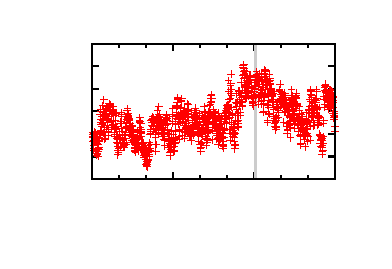
\includegraphics{/home/rik/workspace/ASL_student_project/Repositories/report-fork/Report/images/windminute}}%
    \gplfronttext
  \end{picture}%
\endgroup

	\tiny{Wind speed observations in $[\si{\metre\per\second}$] \cite{www:googleheliostat}.} 
	}
%    \def\figurewidth{{0.5\textwidth}}
%    \def\figureheight{0.6\figurewidth}
\end{minipage}

\clearpage
\ETHslide
\section*{System Overview}
%\addcontentsline{toc}{section}{Control Approach}
\vspace*{\fill}

\begin{figure}[h]
\centering
\scalebox{1}{
%\begin{tikzpicture}[auto, font=\small]
% coordinates
\coordinate (orig) at (0,0);
\coordinate (in1) at (0,-0.75);
\coordinate (in2) at (0,-1.75);
\coordinate (out1) at (12,-1.75/2);
\coordinate (LLA) at (1.5,-1.5);
\coordinate (LLB) at (4,-2.5);
\coordinate (LLC) at (6.5,-1.75);
\coordinate (LLD) at (9,-1.75);
\coordinate (in2inter1) at (1.5,-1.75);
\coordinate (out1inter1) at (11.5,-1.75/2);
\coordinate (out1inter2) at (3,-2.75);


% nodes
\node[draw, minimum width=1.5cm, minimum height=1.5cm, anchor=south west, text width=1.5cm, align=center, fill=red] (A) at (LLA) {Position\\Control};
\node[draw, minimum width=1.5cm, minimum height=2cm, anchor=south west, text width=1.5cm, align=center] (B) at (LLB) {Attitude\\Control};
\node[draw, minimum width=1.5cm, minimum height=1.75cm, anchor=south west, text width=1.5cm, align=center] (C) at (LLC) {Allocation\\Map};
\node[draw, minimum width=1.5cm, minimum height=1.75cm, anchor=south west, text width=1.5cm, align=center] (D) at (LLD) {MAV\\Dynamics};
\coordinate (LLE) at ($(D.270) - (0,1)$);
\node[draw, minimum width=1.5cm, minimum height=1.75cm, anchor=north, text width=1.5cm, align=center] (E) at (LLE) {State\\Estimator};

% edges
\draw[->] (in1) -- node[above] {$\mathbf{r}_{ref},\mathbf{v}_{ref}$} (A.180);

\draw[->] ($(A.0) + (0,0.5)$) -- node[above,very near start] {$T_{ref}$} ($(C.180) + (0,1.25/2)$);
\draw[->] (A.0) -- node[above] {$\phi_{ref}$} ($(B.180) + (0,0.75)$);
\draw[->] ($(A.0) - (0,0.5)$) -- node[above] {$\theta_{ref}$} ($(B.180) + (0,0.25)$);

\draw[-] (in2) -- node[above] {$\psi_{ref}$} (in2inter1);
\draw[->] (in2inter1) -- node {} ($(B.180) -  (0,0.25)$);

\draw[->] (B.0) -- node[above] {$\boldsymbol{\tau}_{ref}$} ($(C.180) - (0,1.25/2)$);

\draw[->] (C.0) -- node[above] {$\mathbf{n}_{ref}$} (D.180);

\draw[-] (D.0) -- node[above] {$\mathbf{y}$} (out1inter1);
\path[fill] (out1inter1) circle[radius=1pt];
\draw[->] (out1inter1) -- node[] {} (out1);

\path[draw,->] (out1inter1) |- (E.0);
\path[draw,->] (E.180) -| node[above,near start] {$\mathbf{r},\mathbf{v},\mathbf{q},\boldsymbol{\omega},\mathbf{w}$} ($(B.270)$) ;

\path[draw,->] (E.180) -| (A.270);

% boxing
\draw [thick, fill=black, opacity=0.5]($(B.180)+(-0.1,-3.25)$) rectangle (11.75,0.25);
\node[right] at (4,-4.5) {Black Box};

\end{tikzpicture}

\begin{tikzpicture}[auto, font=\small]
% coordinates
\coordinate (orig) at (0,0);
\coordinate (LLA) at (2,0);
\coordinate (LLB) at (5.5,0);
\coordinate (outinter) at (8,0);
\coordinate (out) at (9,0);


% nodes
\node[draw, minimum width=1.5cm, minimum height=1.5cm, anchor=west, text width=1.5cm, align=center] (A) at (LLA) {Position\\Control};
\node[draw, minimum width=1.5cm, minimum height=1.5cm, anchor=west, text width=1.5cm, align=center,fill=black,opacity=0.6] (B) at (LLB) {MAV \\Black Box};

% edges
\draw[->] (orig) -- node[above] {$\mathbf{r}_{ref},\mathbf{v}_{ref},\psi_{ref}$} (A.180);
\draw[->] (A.0) -- node[above] {$\begin{bmatrix}
T_{ref} \\ \phi_{ref} \\ \theta_{ref} \\ \psi_{ref}
\end{bmatrix}$} (B.180);
\draw[->] (B.0) -- (out);
\coordinate (feedback) at ($(A.270)-(0,0.75)$);
\draw[-] (outinter) |- node[above,near end] {$\mathbf{r},\mathbf{v},\mathbf{q},\boldsymbol{\omega},\mathbf{w}$} (feedback);
\draw[->] (feedback) -- (A.270);

\end{tikzpicture}

}
\end{figure}
\begin{itemize}
\item[\ETHitem] Cascaded control
\item[\ETHitem] Given attitude control
\item[\ETHitem] Given state and wind estimation
\item[\ETHitem] SysId attitude and thrust dynamics
\end{itemize}

\vspace*{\fill}
\clearpage
\ETHslide
\section*{Control System}
%\addcontentsline{toc}{section}{Control System}
\vspace*{\fill}
\begin{figure}[h]
\centering
\scalebox{0.5}{
\begin{tikzpicture}[auto, font=\small]
% coordinates
\coordinate (orig) at (0,0);
% inputs
\coordinate (Tin) at (orig);
\coordinate (phiin) at ($(orig)- (0,1.75)$);
\coordinate (thetain) at ($(phiin)- (0,1.75)$);
\coordinate (psiin) at ($(thetain)- (0,1.75)$);
% boxes
\coordinate (LLA) at ($(Tin) + (0.75,-0.75)$);
\coordinate (LLB) at ($(phiin) + (0.75,-0.75)$);
\coordinate (LLC) at ($(thetain) + (0.75,-0.75)$);
\coordinate (LLD) at ($(LLC) + (1.5+1.25,0)$);

% nodes
% boxes
\node[draw,minimum width=1.5cm, minimum height=1.5cm, anchor=south west, text width=1.5cm, align=center] (A) at (LLA) {$\Large 1$};
\node[draw,minimum width=1.5cm, minimum height=1.5cm, anchor=south west, text width=1.5cm, align=center] (B) at (LLB) {$G_{\phi_{ref} \rightarrow \phi}$};
\node[draw,minimum width=1.5cm, minimum height=1.5cm, anchor=south west, text width=1.5cm, align=center] (C) at (LLC) {$G_{\theta_{ref} \rightarrow \theta}$};
\node[draw,minimum width=3cm, minimum height=3.25cm, anchor=south west, align=center] (D) at (LLD) {$\frac{1}{m} \left( \rotWB \displaystyle \sum_{i=1}^n \left(\mathbf{F}_{T,i} + \mathbf{F}_{D,i} \right) + \mathbf{F}_G \right)$};

\node[draw,minimum width=0.75cm, minimum height=0.75cm, anchor=west, text width=0.75cm, align=center] (E) at ($(D.0) + (0.5,0)$) {$\Large \int$};
\node[draw,minimum width=0.75cm, minimum height=0.75cm, anchor=west, text width=0.75cm, align=center] (F) at ($(E.0) + (0.5,0)$) {$\Large \int$};
% coordinates at boxes
\coordinate (DTin) at ($(D.180) + (0,2*0.55)$);
\coordinate (Dphiin) at ($(D.180) + (0,1*0.55)$);
\coordinate (Dthetain) at ($(D.180)$);
\coordinate (Dpsiin) at ($(D.180) - (0,1*0.55)$);
\coordinate (Ddxin) at ($(D.180) - (0,2*0.55)$);
\coordinate[above=of D.90] (win);
%lines
\draw[->] (Tin) -- node[at start,above]{$T_{ref}$} (A.180);
\draw[->] (phiin) -- node[at start,above]{$\phi_{ref}$} (B.180);
\draw[->] (thetain) -- node[at start,above]{$\theta_{ref}$} (C.180);
\draw[->] (A.0) -| node[near start,above]{$T$} ($(DTin) - (0.5,0)$) -- (DTin);
\draw[->] (B.0) -| node[near start,above]{$\phi$} ($(Dphiin) - (0.5,0)$) --  (Dphiin);
\draw[->] (C.0) -| node[near start,above]{$\theta$} ($(Dthetain) - (0.75,0)$) -- (Dthetain);
\draw[->] (psiin) -| node[at start,above]{$\psi_{m}$} ($(Dpsiin) - (0.5,0)$) -- (Dpsiin);

\draw[->] (D.0) -- node[above]{${\mathbf{a}}$} (E.180);
\draw[->] (E.0) -- node[above]{${\mathbf{v}}$} (F.180);
\coordinate (out) at ($(F.0) + (0.5,0)$);
\draw[->] (F.0) -- node[above]{$\mathbf{r}$} (out);

\draw[->] ($(E.0) + (0.5/2,0)$) |- ($(D.south west) - (0.25,0.5)$) |- (Ddxin);

\draw[->] (win) node[above]{$\E[\mathbf{w}]$}  -- (D.90);


\end{tikzpicture}

}
\end{figure}
\tiny{
\begin{align}
f\left(\mathbf{x},\mathbf{u},\mathbf{w}\right) &= \ddt \mathbf{x}  
= \begin{bmatrix}
\mathbf{A}_\phi \begin{bmatrix}
\frac{1}{8}\dot{\phi} \\ \phi
\end{bmatrix}
+ \mathbf{B}_\phi \phi_{ref} \\
\mathbf{A}_\theta \begin{bmatrix}
\frac{1}{8}\dot{\theta} \\ \theta
\end{bmatrix}
+ \mathbf{B}_\theta \theta_{ref} \\
\mathbf{v}\\
\frac{1}{m} \left( \mathbf{F}_{T,total} + \mathbf{F}_{D,total} \right)  + \begin{bmatrix}
0 \\ 0 \\ -g
\end{bmatrix} 
\end{bmatrix} \nonumber
\end{align}
}
\normalsize{}

%\begin{minipage}{0.6\textwidth}
%\end{minipage}
%\begin{minipage}{0.39\textwidth}
%\end{minipage}

\vspace*{\fill}
\clearpage
\addcontentsline{toc}{section}{Control}
\ETHslide
\section*{Receding Horizon Control}
%\addcontentsline{toc}{section}{}
\vspace*{\fill}

\begin{figure}[h]
\centering
\scalebox{0.6}{
\begin{tikzpicture}[auto, font=\small]
% coordinates
\coordinate (orig) at (0,0);
\coordinate (LLA) at (orig);
\coordinate (LLB) at (6.5,0);
\coordinate (out) at (12.5,0);


% nodes
\node[draw, minimum width=5cm, minimum height = 4cm, anchor=west, text width=5cm,align=center] (A) at (LLA) {\begin{align*}
&\argmin_{U_t}&  &\sum_{k=0}^{N-1} q(x_{t+k},u_{t+k}) \\
&\text{s.t.}  &  &x_t = x(t) \\
&	          &  &x_{t+k+1} = Ax_{t+k} + Bu_{t+k} \\
&	          &  &x_{t+k}\in\mathcal{X}, \; u_{t+k}\in\mathcal{U}
\end{align*}};
\node[draw, minimum width=4cm, minimum height = 4cm, anchor=west, text width=4cm,align=center] (B) at (LLB) {\Huge{\text{Plant}}};

% edges
\draw[->] (A.0) -- node[above] {$u^*_t$} (B.180);
\draw[->] (B.0) -- node[above] {Output $y(t)$} (out);
\coordinate (stateinter) at ($(A.270) - (0,1)$);
\draw[-] (B.270) |- node[near end, above] {State $x(t)$} (stateinter);
\draw[->] (stateinter) -- (A.270);


% edges
%\draw[->] (in1) -- node[above] {$\mathbf{r}_{ref},\mathbf{v}_{ref}$} (A.180);
%
%\draw[->] ($(A.0) + (0,0.5)$) -- node[above] {$T_{ref}$} ($(C.180) + (0,1.25/2)$);
%\draw[->] (A.0) -- node[above] {$\phi_{ref}$} ($(B.180) + (0,0.75)$);
%\draw[->] ($(A.0) - (0,0.5)$) -- node[above] {$\theta_{ref}$} ($(B.180) + (0,0.25)$);
%
%\draw[-] (in2) -- node[above] {$\psi_{ref}$} (in2inter1);
%\draw[->] (in2inter1) -- node {} ($(B.180) -  (0,0.25)$);
%
%\draw[->] (B.0) -- node[above] {$\boldsymbol{\tau}_{ref}$} ($(C.180) - (0,1.25/2)$);
%
%\draw[->] (C.0) -- node[above] {$\mathbf{n}_{ref}$} (D.180);
%
%\draw[-] (D.0) -- node[] {} (out1inter1);
%\path[fill] (out1inter1) circle[radius=1pt];
%\draw[->] (out1inter1) -- node[] {} (out1);
%
%\path[draw,-] (out1inter1) |- node[near end,below] {$\mathbf{x},\mathbf{\dot{x}},\mathbf{q},\boldsymbol{\omega}$} (out1inter2) ;
%\path[draw,->] (out1inter2) |- ($(B.180) - (0,0.75)$) ;
%\path[draw,->] (out1inter2) -| ($(A.270)$) ;

\end{tikzpicture}
}
\end{figure} 
At each sample time:
\begin{itemize}
\item[\ETHitem] Measure/estimate current state $x(t)$
\item[\ETHitem] Find the optimal input sequence for the entire planning window $N$: $U_t^* = \{ u_t^*, u_{t+1}^*, \ldots, u_{t+N-1}^* \}$
\item[\ETHitem] Implement the first control action $u_t^*$
\end{itemize}

\vspace*{\fill}
\clearpage
\ETHslide
\section*{Receding Horizon Control}
%\addcontentsline{toc}{section}{}
\vspace*{\fill}

Advantages:
\begin{itemize}
\item[\ETHitem] Input and output constraints
\item[\ETHitem] Predictive
\item[\ETHitem] Intuitive
\end{itemize}
Disadvantages:
\begin{itemize}
\item[\ETHitem] No robustness guarantees
\item[\ETHitem] OCP computationally expensive
\end{itemize}

\vspace*{\fill}
\clearpage
%\ETHslide
\section*{Linear MPC}
%\addcontentsline{toc}{section}{}
\vspace*{\fill}

\begin{itemize}
\item[\ETHitem] \underline{Linearization}: About hovering
\item[\ETHitem] \underline{Offset-free}: System augmented with constant input disturbance 
\item[\ETHitem] \underline{Constant Disturbances}: Estimated with Luenberger observer
\item[\ETHitem] \underline{Reference tracking}: Tracking all $N$ future reference positions and velocities (feed-forward)
\item[\ETHitem] \underline{Input constraints}: Limited thrust, roll and pitch
\item[\ETHitem] \underline{Terminal penalty $P$}: Solution of algebraic Riccati equation
\item[\ETHitem] \underline{CVXGEN}: Generate hard-coded convex optimization solver
\end{itemize}

\vspace*{\fill}
\clearpage
%\ETHslide
\section*{Linear MPC OCP}
%\addcontentsline{toc}{section}{}
\footnotesize{
\begin{align}
&\min_{u(\cdot),x(\cdot)}
& & ||x_N-\bar{x}_t||_P^2 + \sum_{k=0}^{N-1} ||x_k - \bar{x}_t||_Q^2 + ||u_k - \bar{u}_t||_R^2  \nonumber\\
& \text{s.t.} 
& & x_{k+1} = A x_k + B u_k + B_w w_k + B_d d_k, & k = 0, \ldots, N-1 \nonumber\\
& & & w_{k+1} = w_k  & k = 0, \ldots, N-1 \nonumber\\
& & & d_{k+1} = d_k, & k = 0, \ldots, N-1 \nonumber\\
& & & \begin{bmatrix}
T_{min} \\ -30\si{\degree} \\ -30\si{\degree}
\end{bmatrix} \leq u_k \leq \begin{bmatrix}
T_{max} \\ 30\si{\degree} \\ 30\si{\degree}
\end{bmatrix} & k = 0, \ldots, N-1 \nonumber\\
& & & x_0 = \hat x (t), \; d_0 = \hat d(t), \; w_0 = \hat w(t) \nonumber \\
& & & N=40 \nonumber
\end{align}
}
\normalsize{}
\clearpage
%\ETHslide
\section*{Linear MPC Algorithm}
%\addcontentsline{toc}{section}{}
\vspace*{\fill}

At every sample time:
\begin{itemize}
\item[\ETHitem] Update state $\hat{x}(t)$ and disturbance $\hat{d}(t)$ estimation
\item[\ETHitem] Calculate $N+1$ desired steady-state inputs $\bar{u}_t$ and states $\bar{x}_t$
\item[\ETHitem] Solve finite-horizon optimal control problem (CVXGEN)
\item[\ETHitem] Apply first optimal control action to system
\end{itemize}

\vspace*{\fill}
\clearpage
%\ETHslide
\section*{Nonlinear MPC}
%\addcontentsline{toc}{section}{}
\vspace*{\fill}
No stability guarantees, no optimality guarantees
\begin{itemize}
\item[\ETHitem] \underline{Offset-free}: System augmented with integrator
\item[\ETHitem] \underline{Reference tracking}: Tracking all $N$ future reference positions and velocities (feed-forward)
\item[\ETHitem] \underline{Input constraints}: Limited thrust, roll and pitch
\item[\ETHitem] \underline{Terminal penalty P}: Solution of algebraic Riccati equation of linearized system
\item[\ETHitem] \underline{ACADO}: Generate hard-coded nonlinear optimization solver
\item[\ETHitem] \underline{qpDUNES}: Interior point method/active set for solving sparse OCP
\end{itemize}

\vspace*{\fill}
\clearpage
\input{slides/12_nonlinear_mpc_ocp}
%\ETHslide
\section*{Nonlinear MPC Algorithm}
%\addcontentsline{toc}{section}{}
\vspace*{\fill}

At every sample time:
\begin{itemize}
\item[\ETHitem] Set current state, wind and heading
\item[\ETHitem] Set $N+1$ references
\item[\ETHitem] Set previous optimal solution as warm start
\item[\ETHitem] Solve finite-horizon optimal control problem (ACADO)
\item[\ETHitem] Update integrator
\item[\ETHitem] Apply first optimal control action to system
\end{itemize}

\vspace*{\fill}
\clearpage
%\ETHslide
\section*{Step Response: Linear MPC}
%\addcontentsline{toc}{section}{}
\vspace*{\fill}

\begin{minipage}{0.5\textwidth}
	\centering
	\tiny{
	% This file was created by matlab2tikz.
% Minimal pgfplots version: 1.3
%
\definecolor{mycolor1}{rgb}{0.00000,0.44700,0.74100}%
\definecolor{mycolor2}{rgb}{0.85000,0.32500,0.09800}%
\definecolor{mycolor3}{rgb}{0.92900,0.69400,0.12500}%
%
\begin{tikzpicture}

\begin{axis}[%
width=\figurewidth,
height=0.984009\figureheight,
at={(0\figurewidth,0\figureheight)},
scale only axis,
xmin=0,
xmax=5,
xlabel={time $[\si{\second}]$},
ymin=-0.2,
ymax=1.2,
ylabel={position $[\si{\metre}]$},
axis x line*=bottom,
axis y line*=left,
legend style={at={(0.5,1.03)},anchor=south,legend columns=3,legend cell align=left,align=left,draw=white!15!black}
]
\addplot [color=mycolor1,solid]
  table[row sep=crcr]{%
0	0\\
0.01	1.14690425758758e-08\\
0.02	3.9139247376254e-07\\
0.03	2.83493392441896e-06\\
0.04	1.11051834900563e-05\\
0.05	3.12788497901201e-05\\
0.06	7.18257334289189e-05\\
0.07	0.000143559484600181\\
0.08	0.000259428712558198\\
0.09	0.000434230940921711\\
0.1	0.000684297077484614\\
0.11	0.00102717519265354\\
0.12	0.00148133123930672\\
0.13	0.00206587644600224\\
0.14	0.00280032594689838\\
0.15	0.00370439000250268\\
0.16	0.0047977972180332\\
0.17	0.00610014799051753\\
0.18	0.00763079651509766\\
0.19	0.00940876480511783\\
0.2	0.0114526846522818\\
0.21	0.0137807407968232\\
0.22	0.0164106284954103\\
0.23	0.0193595249032115\\
0.24	0.0226440708237129\\
0.25	0.0262803601235094\\
0.26	0.0302839346288481\\
0.27	0.0346698148326636\\
0.28	0.0394526012157968\\
0.29	0.044646482601358\\
0.3	0.0502656879782431\\
0.31	0.0563257286016026\\
0.32	0.0628426614025463\\
0.33	0.0698305493531942\\
0.34	0.0773002587755007\\
0.35	0.0852591459937297\\
0.36	0.0937110624737891\\
0.37	0.10265645737235\\
0.38	0.112092670157311\\
0.39	0.122014712549827\\
0.4	0.132415897683296\\
0.41	0.143287379804692\\
0.42	0.154617504758948\\
0.43	0.166391506536651\\
0.44	0.178591430063641\\
0.45	0.191196207501871\\
0.46	0.204181846842149\\
0.47	0.217521705701489\\
0.48	0.231186839716325\\
0.49	0.245146401191358\\
0.5	0.259368025637102\\
0.51	0.273818231820918\\
0.52	0.288462828823561\\
0.53	0.303267317616087\\
0.54	0.318197276391322\\
0.55	0.333218720529993\\
0.56	0.348298429762913\\
0.57	0.363404236834843\\
0.58	0.37850527376272\\
0.59	0.393572173563614\\
0.6	0.408577227045264\\
0.61	0.423494495838767\\
0.62	0.438299884244244\\
0.63	0.452971173597493\\
0.64	0.467488023671323\\
0.65	0.481831943133623\\
0.66	0.495986218252608\\
0.67	0.509935817073701\\
0.68	0.523667306773268\\
0.69	0.537168771172672\\
0.7	0.550429646962763\\
0.71	0.563440613862694\\
0.72	0.576193589079729\\
0.73	0.58868171088866\\
0.74	0.6008992960234\\
0.75	0.612841777357085\\
0.76	0.624505646924077\\
0.77	0.635888407683714\\
0.78	0.646988518112545\\
0.79	0.657805330684049\\
0.8	0.668339026920506\\
0.81	0.678590550676979\\
0.82	0.688561540863623\\
0.83	0.698254264592939\\
0.84	0.707671551606085\\
0.85	0.716816730725328\\
0.86	0.725693568974922\\
0.87	0.734306213903445\\
0.88	0.742659139527276\\
0.89	0.750757096200328\\
0.9	0.758605064603075\\
0.91	0.766208213937729\\
0.92	0.773571864319226\\
0.93	0.7807014532656\\
0.94	0.787602506118118\\
0.95	0.79428061016196\\
0.96	0.800741392172575\\
0.97	0.806990499080787\\
0.98	0.813033580514812\\
0.99	0.818876272806302\\
1	0.824524185901435\\
1.01	0.829982894661978\\
1.02	0.835257931695948\\
1.03	0.840354781017045\\
1.04	0.845278872297848\\
1.05	0.850035575522238\\
1.06	0.854630196208461\\
1.07	0.859067970746821\\
1.08	0.863354061992374\\
1.09	0.867493555060194\\
1.1	0.871491453182171\\
1.11	0.87535267357497\\
1.12	0.879082043435866\\
1.13	0.882684296044236\\
1.14	0.886164066941702\\
1.15	0.889525890212335\\
1.16	0.892774194894376\\
1.17	0.895913301554866\\
1.18	0.89894741902765\\
1.19	0.901880641396319\\
1.2	0.904716945274591\\
1.21	0.907460187348123\\
1.22	0.910114102235678\\
1.23	0.912682300757355\\
1.24	0.915168268599074\\
1.25	0.917575365368301\\
1.26	0.91990682406119\\
1.27	0.922165750954413\\
1.28	0.924355125928457\\
1.29	0.926477803223071\\
1.3	0.928536512619652\\
1.31	0.930533861039892\\
1.32	0.932472334512499\\
1.33	0.934354300260928\\
1.34	0.936182009135477\\
1.35	0.937957598820566\\
1.36	0.939683097826402\\
1.37	0.941360429681311\\
1.38	0.942991417158007\\
1.39	0.944577786539642\\
1.4	0.946121171929167\\
1.41	0.94762311958439\\
1.42	0.949085092253852\\
1.43	0.95050847348715\\
1.44	0.951894571894401\\
1.45	0.953244625331588\\
1.46	0.954559804967361\\
1.47	0.955841219192675\\
1.48	0.957089917465828\\
1.49	0.95830689408983\\
1.5	0.959493091809487\\
1.51	0.960649405225339\\
1.52	0.961776684031765\\
1.53	0.962875736081455\\
1.54	0.963947330277348\\
1.55	0.964992199293578\\
1.56	0.966011042127964\\
1.57	0.967004526489633\\
1.58	0.967973291026402\\
1.59	0.968917947397434\\
1.6	0.969839082197384\\
1.61	0.970737258738867\\
1.62	0.971613018700483\\
1.63	0.972466883647928\\
1.64	0.97329935643587\\
1.65	0.974110922498328\\
1.66	0.974902051034955\\
1.67	0.975673196093077\\
1.68	0.976424797558711\\
1.69	0.977157282068922\\
1.7	0.977871063849827\\
1.71	0.978566545483366\\
1.72	0.979244118610003\\
1.73	0.979904164573894\\
1.74	0.980547055017221\\
1.75	0.981173152429806\\
1.76	0.981782810659678\\
1.77	0.982376375387689\\
1.78	0.982954184569631\\
1.79	0.983516568848525\\
1.8	0.984063851939205\\
1.81	0.98459635098693\\
1.82	0.985114376901473\\
1.83	0.985618234667903\\
1.84	0.986108223635136\\
1.85	0.986584637783194\\
1.86	0.987047765970034\\
1.87	0.987497892158757\\
1.88	0.987935295625965\\
1.89	0.988360251152017\\
1.9	0.988773029193527\\
1.91	0.989173896039905\\
1.92	0.989563113954603\\
1.93	0.989940941301279\\
1.94	0.990307632655264\\
1.95	0.990663438902003\\
1.96	0.991008607323251\\
1.97	0.991343381671389\\
1.98	0.991668002232454\\
1.99	0.991982705879022\\
2	0.992287726114213\\
2.01	0.992583293107279\\
2.02	0.992869633721411\\
2.03	0.993146971534488\\
2.04	0.993415526853936\\
2.05	0.993675516726601\\
2.06	0.993927154944095\\
2.07	0.994170652044259\\
2.08	0.994406215309351\\
2.09	0.994634048761547\\
2.1	0.994854353156842\\
2.11	0.995067325977704\\
2.12	0.995273161424908\\
2.13	0.995472050409008\\
2.14	0.995664180541957\\
2.15	0.995849736129257\\
2.16	0.996028898162972\\
2.17	0.996201844315918\\
2.18	0.99636874893754\\
2.19	0.996529783051571\\
2.2	0.996685114355665\\
2.21	0.996834907223171\\
2.22	0.996979322707083\\
2.23	0.997118518546175\\
2.24	0.997252649173727\\
2.25	0.997381865729044\\
2.26	0.99750631607147\\
2.27	0.997626144796828\\
2.28	0.997741493256335\\
2.29	0.997852499577948\\
2.3	0.997959298690065\\
2.31	0.998062022347525\\
2.32	0.998160799159841\\
2.33	0.998255754621606\\
2.34	0.998347011144909\\
2.35	0.998434688093666\\
2.36	0.998518901819783\\
2.37	0.998599765701016\\
2.38	0.998677390180386\\
2.39	0.998751882807035\\
2.4	0.998823348278413\\
2.41	0.998891888483678\\
2.42	0.998957602548179\\
2.43	0.999020586878969\\
2.44	0.999080935211246\\
2.45	0.999138738655606\\
2.46	0.999194085746011\\
2.47	0.999247062488347\\
2.48	0.999297752409465\\
2.49	0.999346236606577\\
2.5	0.999392593796917\\
2.51	0.999436900367539\\
2.52	0.999479230425164\\
2.53	0.999519655845981\\
2.54	0.999558246325312\\
2.55	0.999595069427053\\
2.56	0.999630190632842\\
2.57	0.999663673390859\\
2.58	0.999695579164216\\
2.59	0.99972596747887\\
2.6	0.999754895971014\\
2.61	0.999782420433913\\
2.62	0.999808594864135\\
2.63	0.999833471507161\\
2.64	0.999857100902338\\
2.65	0.999879531927163\\
2.66	0.999900811840885\\
2.67	0.999920986327398\\
2.68	0.999940099537431\\
2.69	0.999958194130019\\
2.7	0.999975311313261\\
2.71	0.999991490884347\\
2.72	1.00000677126887\\
2.73	1.0000211895594\\
2.74	1.00003478155337\\
2.75	1.00004758179019\\
2.76	1.00005962358774\\
2.77	1.00007093907802\\
2.78	1.00008155924222\\
2.79	1.00009151394502\\
2.8	1.00010083196819\\
2.81	1.0001095410435\\
2.82	1.0001176678849\\
2.83	1.00012523822003\\
2.84	1.00013227682103\\
2.85	1.00013880753467\\
2.86	1.00014485331174\\
2.87	1.00015043623588\\
2.88	1.00015557755159\\
2.89	1.00016029769167\\
2.9	1.00016461630395\\
2.91	1.00016855227737\\
2.92	1.00017212376735\\
2.93	1.00017534822059\\
2.94	1.00017824239919\\
2.95	1.00018082240403\\
2.96	1.00018310369766\\
2.97	1.00018510112642\\
2.98	1.00018682894197\\
2.99	1.00018830082224\\
3	1.0001895298917\\
3.01	1.00019052874104\\
3.02	1.00019130944627\\
3.03	1.00019188358723\\
3.04	1.00019226226551\\
3.05	1.00019245612184\\
3.06	1.00019247535289\\
3.07	1.00019232972757\\
3.08	1.00019202860275\\
3.09	1.00019158093855\\
3.1	1.00019099531308\\
3.11	1.00019027993667\\
3.12	1.00018944266568\\
3.13	1.00018849101585\\
3.14	1.00018743217512\\
3.15	1.00018627301615\\
3.16	1.00018502010826\\
3.17	1.00018367972914\\
3.18	1.00018225787599\\
3.19	1.00018076027637\\
3.2	1.00017919239868\\
3.21	1.00017755946223\\
3.22	1.00017586644697\\
3.23	1.00017411810293\\
3.24	1.00017231895925\\
3.25	1.00017047333292\\
3.26	1.00016858533726\\
3.27	1.00016665889001\\
3.28	1.00016469772118\\
3.29	1.00016270538063\\
3.3	1.00016068524532\\
3.31	1.00015864052636\\
3.32	1.00015657427575\\
3.33	1.00015448939287\\
3.34	1.00015238863081\\
3.35	1.00015027460233\\
3.36	1.00014814978574\\
3.37	1.00014601653043\\
3.38	1.00014387706228\\
3.39	1.00014173348882\\
3.4	1.00013958780423\\
3.41	1.00013744189408\\
3.42	1.00013529753998\\
3.43	1.00013315642394\\
3.44	1.00013102013269\\
3.45	1.00012889016172\\
3.46	1.00012676791919\\
3.47	1.00012465472973\\
3.48	1.00012255183804\\
3.49	1.00012046041239\\
3.5	1.00011838154793\\
3.51	1.00011631626989\\
3.52	1.00011426553669\\
3.53	1.00011223024288\\
3.54	1.00011021122194\\
3.55	1.00010820924908\\
3.56	1.00010622504376\\
3.57	1.00010425927227\\
3.58	1.00010231255009\\
3.59	1.00010038544424\\
3.6	1.00009847847545\\
3.61	1.00009659212034\\
3.62	1.00009472681339\\
3.63	1.00009288294898\\
3.64	1.0000910608832\\
3.65	1.00008926093571\\
3.66	1.0000874833914\\
3.67	1.00008572850213\\
3.68	1.00008399648828\\
3.69	1.00008228754026\\
3.7	1.00008060182002\\
3.71	1.00007893946243\\
3.72	1.00007730057664\\
3.73	1.00007568524737\\
3.74	1.00007409353615\\
3.75	1.00007252548251\\
3.76	1.00007098110515\\
3.77	1.00006946040299\\
3.78	1.00006796335626\\
3.79	1.00006648992748\\
3.8	1.00006504006245\\
3.81	1.00006361369118\\
3.82	1.00006221072874\\
3.83	1.00006083107616\\
3.84	1.00005947462122\\
3.85	1.00005814123923\\
3.86	1.0000568307938\\
3.87	1.00005554313753\\
3.88	1.00005427811274\\
3.89	1.00005303555208\\
3.9	1.00005181527921\\
3.91	1.00005061710935\\
3.92	1.00004944084993\\
3.93	1.00004828630106\\
3.94	1.00004715325615\\
3.95	1.00004604150233\\
3.96	1.00004495082101\\
3.97	1.0000438809883\\
3.98	1.00004283177547\\
3.99	1.00004180294935\\
4	1.0000407942728\\
4.01	1.00003980550501\\
4.02	1.00003883640193\\
4.03	1.00003788671663\\
4.04	1.00003695619958\\
4.05	1.00003604459902\\
4.06	1.00003515166127\\
4.07	1.00003427713099\\
4.08	1.00003342075149\\
4.09	1.00003258226496\\
4.1	1.00003176141278\\
4.11	1.00003095793569\\
4.12	1.00003017157409\\
4.13	1.00002940206821\\
4.14	1.00002864915832\\
4.15	1.00002791258496\\
4.16	1.0000271920891\\
4.17	1.00002648741231\\
4.18	1.00002579829695\\
4.19	1.00002512448633\\
4.2	1.00002446572482\\
4.21	1.00002382175805\\
4.22	1.000023192333\\
4.23	1.00002257719815\\
4.24	1.00002197610358\\
4.25	1.0000213888011\\
4.26	1.00002081504434\\
4.27	1.00002025458886\\
4.28	1.00001970719224\\
4.29	1.00001917261417\\
4.3	1.0000186506165\\
4.31	1.00001814096336\\
4.32	1.0000176434212\\
4.33	1.00001715775887\\
4.34	1.00001668374765\\
4.35	1.00001622116135\\
4.36	1.00001576977633\\
4.37	1.00001532937152\\
4.38	1.00001489972855\\
4.39	1.00001448063167\\
4.4	1.00001407186787\\
4.41	1.00001367322689\\
4.42	1.00001328450122\\
4.43	1.00001290548614\\
4.44	1.00001253597976\\
4.45	1.00001217578299\\
4.46	1.0000118246996\\
4.47	1.00001148253619\\
4.48	1.00001114910224\\
4.49	1.00001082421007\\
4.5	1.00001050767488\\
4.51	1.00001019931473\\
4.52	1.00000989895055\\
4.53	1.00000960640612\\
4.54	1.00000932150808\\
4.55	1.00000904408591\\
4.56	1.00000877397194\\
4.57	1.0000085110013\\
4.58	1.00000825501196\\
4.59	1.00000800584467\\
4.6	1.00000776334297\\
4.61	1.00000752735314\\
4.62	1.00000729772424\\
4.63	1.00000707430803\\
4.64	1.00000685695898\\
4.65	1.00000664553424\\
4.66	1.00000643989363\\
4.67	1.00000623989958\\
4.68	1.00000604541716\\
4.69	1.000005856314\\
4.7	1.0000056724603\\
4.71	1.00000549372877\\
4.72	1.00000531999465\\
4.73	1.00000515113563\\
4.74	1.00000498703186\\
4.75	1.00000482756589\\
4.76	1.00000467262267\\
4.77	1.00000452208949\\
4.78	1.00000437585598\\
4.79	1.00000423381406\\
4.8	1.00000409585789\\
4.81	1.00000396188389\\
4.82	1.00000383179066\\
4.83	1.00000370547897\\
4.84	1.00000358285174\\
4.85	1.00000346381396\\
4.86	1.00000334827273\\
4.87	1.00000323613716\\
4.88	1.00000312731837\\
4.89	1.00000302172947\\
4.9	1.0000029192855\\
4.91	1.00000281990341\\
4.92	1.00000272350202\\
4.93	1.00000263000202\\
4.94	1.0000025393259\\
4.95	1.00000245139792\\
4.96	1.00000236614411\\
4.97	1.00000228349221\\
4.98	1.00000220337166\\
4.99	1.00000212571355\\
5	1.00000205045059\\
};
\addlegendentry{x};

\addplot [color=mycolor2,solid]
  table[row sep=crcr]{%
0	0\\
0.01	-1.55177660043528e-23\\
0.02	-2.67274574431345e-13\\
0.03	-8.98478263104176e-12\\
0.04	-6.16971360850354e-11\\
0.05	-2.2297262599863e-10\\
0.06	-5.63143026467177e-10\\
0.07	-1.12284298361237e-09\\
0.08	-1.88432511755817e-09\\
0.09	-2.76567687508838e-09\\
0.1	-3.64552946441174e-09\\
0.11	-4.41845777422109e-09\\
0.12	-5.07566267856705e-09\\
0.13	-5.8022177532598e-09\\
0.14	-7.08094738967342e-09\\
0.15	-9.79335376595711e-09\\
0.16	-1.53093607479971e-08\\
0.17	-2.55595124262953e-08\\
0.18	-4.30855042456767e-08\\
0.19	-7.10706674426555e-08\\
0.2	-1.13348156435952e-07\\
0.21	-1.74371887537051e-07\\
0.22	-2.59154892994293e-07\\
0.23	-3.73184505633744e-07\\
0.24	-5.22321304450265e-07\\
0.25	-7.12687183644643e-07\\
0.26	-9.50546848844114e-07\\
0.27	-1.24219077730769e-06\\
0.28	-1.59382668232799e-06\\
0.29	-2.01145696563217e-06\\
0.3	-2.50083839741196e-06\\
0.31	-3.06760240797529e-06\\
0.32	-3.71707167725793e-06\\
0.33	-4.45375845931693e-06\\
0.34	-5.28110164802155e-06\\
0.35	-6.2013868806401e-06\\
0.36	-7.21574575886128e-06\\
0.37	-8.32418173750178e-06\\
0.38	-9.52562808564532e-06\\
0.39	-1.08180840114527e-05\\
0.4	-1.21986976671083e-05\\
0.41	-1.36636215405781e-05\\
0.42	-1.52078212511313e-05\\
0.43	-1.68249449506927e-05\\
0.44	-1.85072365635161e-05\\
0.45	-2.02454859514349e-05\\
0.46	-2.20290156011993e-05\\
0.47	-2.38457057545927e-05\\
0.48	-2.56820535053694e-05\\
0.49	-2.7523249500673e-05\\
0.5	-2.93532879262815e-05\\
0.51	-3.11551278793805e-05\\
0.52	-3.29109039961258e-05\\
0.53	-3.46021804032711e-05\\
0.54	-3.62102398147108e-05\\
0.55	-3.77163976172807e-05\\
0.56	-3.91023293216542e-05\\
0.57	-4.03503989586696e-05\\
0.58	-4.14439759662762e-05\\
0.59	-4.23677288447864e-05\\
0.6	-4.31078852893436e-05\\
0.61	-4.36524505040723e-05\\
0.62	-4.39913777799745e-05\\
0.63	-4.41166879710807e-05\\
0.64	-4.4022536979539e-05\\
0.65	-4.37052284723403e-05\\
0.66	-4.31631549803496e-05\\
0.67	-4.23966926793223e-05\\
0.68	-4.14080953210245e-05\\
0.69	-4.0201372108246e-05\\
0.7	-3.87820764274962e-05\\
0.71	-3.71571458276573e-05\\
0.72	-3.53348196710979e-05\\
0.73	-3.33245214406003e-05\\
0.74	-3.11367042307167e-05\\
0.75	-2.87826571303649e-05\\
0.76	-2.62742808490266e-05\\
0.77	-2.36238982191234e-05\\
0.78	-2.08441046481987e-05\\
0.79	-1.79476467740375e-05\\
0.8	-1.49473233722516e-05\\
0.81	-1.18559048272061e-05\\
0.82	-8.68606847721948e-06\\
0.83	-5.45034752712645e-06\\
0.84	-2.16109133746943e-06\\
0.85	1.16956506379163e-06\\
0.86	4.52972435129838e-06\\
0.87	7.90774515517454e-06\\
0.88	1.12922570310589e-05\\
0.89	1.46721737566446e-05\\
0.9	1.80367062948586e-05\\
0.91	2.13753764675059e-05\\
0.92	2.46780320774217e-05\\
0.93	2.79348639181285e-05\\
0.94	3.1136424831428e-05\\
0.95	3.42736507260171e-05\\
0.96	3.73378832616531e-05\\
0.97	4.03208937381183e-05\\
0.98	4.32149071241458e-05\\
0.99	4.6012623559986e-05\\
1	4.87072356379909e-05\\
1.01	5.12924464175047e-05\\
1.02	5.37624883358501e-05\\
1.03	5.61121417726326e-05\\
1.04	5.83367522237249e-05\\
1.05	6.04322451668551e-05\\
1.06	6.23951380584343e-05\\
1.07	6.42225485817213e-05\\
1.08	6.59121988746599e-05\\
1.09	6.74624153915347e-05\\
1.1	6.88721241051929e-05\\
1.11	7.01408410084991e-05\\
1.12	7.12686582696756e-05\\
1.13	7.22562261213009e-05\\
1.14	7.31047306430977e-05\\
1.15	7.38158678396493e-05\\
1.16	7.43918144833401e-05\\
1.17	7.48351962291226e-05\\
1.18	7.51490535247034e-05\\
1.19	7.53368061328633e-05\\
1.2	7.54022166466045e-05\\
1.21	7.53493532080872e-05\\
1.22	7.5182552206618e-05\\
1.23	7.4906381388617e-05\\
1.24	7.4525603458809e-05\\
1.25	7.40451405260746e-05\\
1.26	7.34700397571762e-05\\
1.27	7.28054405400056e-05\\
1.28	7.20565433986139e-05\\
1.29	7.1228580845552e-05\\
1.3	7.03267903036216e-05\\
1.31	6.93563891796637e-05\\
1.32	6.83225520828487e-05\\
1.33	6.7230389812676e-05\\
1.34	6.60849302353201e-05\\
1.35	6.4891101489701e-05\\
1.36	6.36537177967103e-05\\
1.37	6.23774673860227e-05\\
1.38	6.10669022910793e-05\\
1.39	5.97264297678983e-05\\
1.4	5.83603051437719e-05\\
1.41	5.6972625921854e-05\\
1.42	5.55673269881557e-05\\
1.43	5.41481767878571e-05\\
1.44	5.27187743576218e-05\\
1.45	5.12825471193545e-05\\
1.46	4.98427493470689e-05\\
1.47	4.84024610270873e-05\\
1.48	4.69645869285745e-05\\
1.49	4.55318566267065e-05\\
1.5	4.41068255154299e-05\\
1.51	4.26918765155732e-05\\
1.52	4.12892223072781e-05\\
1.53	3.99009079919933e-05\\
1.54	3.85288141298157e-05\\
1.55	3.71746601195017e-05\\
1.56	3.5840007899629e-05\\
1.57	3.45262659547071e-05\\
1.58	3.32346936119513e-05\\
1.59	3.19664056143293e-05\\
1.6	3.07223769541826e-05\\
1.61	2.95034479497437e-05\\
1.62	2.83103295445746e-05\\
1.63	2.71436088075918e-05\\
1.64	2.60037546091094e-05\\
1.65	2.48911234463552e-05\\
1.66	2.38059653931056e-05\\
1.67	2.27484301849698e-05\\
1.68	2.17185734599793e-05\\
1.69	2.07163630983891e-05\\
1.7	1.97416855572434e-05\\
1.71	1.87943520874167e-05\\
1.72	1.78741047813834e-05\\
1.73	1.69806224715827e-05\\
1.74	1.61135264717885e-05\\
1.75	1.52723861629456e-05\\
1.76	1.44567243984517e-05\\
1.77	1.36660227272053e-05\\
1.78	1.2899726430771e-05\\
1.79	1.21572493674795e-05\\
1.8	1.14379786149317e-05\\
1.81	1.07412789023046e-05\\
1.82	1.0066496824586e-05\\
1.83	9.41296483206426e-06\\
1.84	8.78000498987775e-06\\
1.85	8.16693250406011e-06\\
1.86	7.57305901219492e-06\\
1.87	6.99769563846176e-06\\
1.88	6.44015581445848e-06\\
1.89	5.89975786869395e-06\\
1.9	5.37582738856945e-06\\
1.91	4.86769935109936e-06\\
1.92	4.37472003714186e-06\\
1.93	3.89624874729581e-06\\
1.94	3.4316593232627e-06\\
1.95	2.98034147077236e-06\\
1.96	2.54170189942064e-06\\
1.97	2.11516530153398e-06\\
1.98	1.70017517513649e-06\\
1.99	1.29619449278496e-06\\
2	9.02706229819881e-07\\
2.01	5.19213764313915e-07\\
2.02	1.45241155793293e-07\\
2.03	-2.19666690220209e-07\\
2.04	-5.75943965946514e-07\\
2.05	-9.2400400107407e-07\\
2.06	-1.26423938855455e-06\\
2.07	-1.59702218942254e-06\\
2.08	-1.92270420948325e-06\\
2.09	-2.24161734138587e-06\\
2.1	-2.55407396622661e-06\\
2.11	-2.86036740523562e-06\\
2.12	-3.16077241489888e-06\\
2.13	-3.45554572025588e-06\\
2.14	-3.74492658120674e-06\\
2.15	-4.02913738682897e-06\\
2.16	-4.30838427287259e-06\\
2.17	-4.58285775784168e-06\\
2.18	-4.85273339365374e-06\\
2.19	-5.11817242701403e-06\\
2.2	-5.37932246797859e-06\\
2.21	-5.63631816242578e-06\\
2.22	-5.8892818634403e-06\\
2.23	-6.13832424752011e-06\\
2.24	-6.38354480538523e-06\\
2.25	-6.62503234190936e-06\\
2.26	-6.86286554612671e-06\\
2.27	-7.09711361420269e-06\\
2.28	-7.32783690773088e-06\\
2.29	-7.55508763322548e-06\\
2.3	-7.77891053063549e-06\\
2.31	-7.99934356016813e-06\\
2.32	-8.21641857828746e-06\\
2.33	-8.43016199601746e-06\\
2.34	-8.64059541383743e-06\\
2.35	-8.84773622833281e-06\\
2.36	-9.05159820730264e-06\\
2.37	-9.25219203072844e-06\\
2.38	-9.44952579578951e-06\\
2.39	-9.64360548588338e-06\\
2.4	-9.83443540332788e-06\\
2.41	-1.00220185652061e-05\\
2.42	-1.0206357063212e-05\\
2.43	-1.03874523889031e-05\\
2.44	-1.05653057260969e-05\\
2.45	-1.07399182123916e-05\\
2.46	-1.09112911719551e-05\\
2.47	-1.10794263218111e-05\\
2.48	-1.12443259538738e-05\\
2.49	-1.14059930949471e-05\\
2.5	-1.15644316468209e-05\\
2.51	-1.1719646508478e-05\\
2.52	-1.18716436822729e-05\\
2.53	-1.20204303657979e-05\\
2.54	-1.21660150317739e-05\\
2.55	-1.23084074983775e-05\\
2.56	-1.24476189893757e-05\\
2.57	-1.2583662183573e-05\\
2.58	-1.2716551254502e-05\\
2.59	-1.28463019013803e-05\\
2.6	-1.29729313721322e-05\\
2.61	-1.30964584790982e-05\\
2.62	-1.32169036079202e-05\\
2.63	-1.33342887199873e-05\\
2.64	-1.34486373487479e-05\\
2.65	-1.35599745901338e-05\\
2.66	-1.36683270873077e-05\\
2.67	-1.37737230099164e-05\\
2.68	-1.38761920280273e-05\\
2.69	-1.39757652809215e-05\\
2.7	-1.40724753409316e-05\\
2.71	-1.41663561725243e-05\\
2.72	-1.42574430868524e-05\\
2.73	-1.43457726920399e-05\\
2.74	-1.44313828399759e-05\\
2.75	-1.45143125712532e-05\\
2.76	-1.45946020582054e-05\\
2.77	-1.46722925438251e-05\\
2.78	-1.47474262763385e-05\\
2.79	-1.48200464401775e-05\\
2.8	-1.4890197084103e-05\\
2.81	-1.49579230471496e-05\\
2.82	-1.50232698830046e-05\\
2.83	-1.50862837834242e-05\\
2.84	-1.51470115020437e-05\\
2.85	-1.52055002806108e-05\\
2.86	-1.52617977767292e-05\\
2.87	-1.53159519906252e-05\\
2.88	-1.53680111913439e-05\\
2.89	-1.54180238432944e-05\\
2.9	-1.54660385358293e-05\\
2.91	-1.55121039165619e-05\\
2.92	-1.5556268625604e-05\\
2.93	-1.55985812299898e-05\\
2.94	-1.56390901588894e-05\\
2.95	-1.56778436402219e-05\\
2.96	-1.57148896391633e-05\\
2.97	-1.57502757989466e-05\\
2.98	-1.57840493842686e-05\\
2.99	-1.58162572275421e-05\\
3	-1.58469456781656e-05\\
3.01	-1.58761605549255e-05\\
3.02	-1.59039471015898e-05\\
3.03	-1.59303499457115e-05\\
3.04	-1.59554130606162e-05\\
3.05	-1.59791797305175e-05\\
3.06	-1.60016925186785e-05\\
3.07	-1.60229932385117e-05\\
3.08	-1.60431229275009e-05\\
3.09	-1.60621218238103e-05\\
3.1	-1.60800293454458e-05\\
3.11	-1.6096884071828e-05\\
3.12	-1.61127237276371e-05\\
3.13	-1.61275851687959e-05\\
3.14	-1.61415043704596e-05\\
3.15	-1.61545164168914e-05\\
3.16	-1.61666554931101e-05\\
3.17	-1.61779548782059e-05\\
3.18	-1.61884469402279e-05\\
3.19	-1.61981631325596e-05\\
3.2	-1.62071339917057e-05\\
3.21	-1.62153891364204e-05\\
3.22	-1.62229572681181e-05\\
3.23	-1.62298661725111e-05\\
3.24	-1.62361427224257e-05\\
3.25	-1.62418128817523e-05\\
3.26	-1.62469017104883e-05\\
3.27	-1.62514333708342e-05\\
3.28	-1.62554311343067e-05\\
3.29	-1.62589173898309e-05\\
3.3	-1.62619136527754e-05\\
3.31	-1.62644405748913e-05\\
3.32	-1.62665179551185e-05\\
3.33	-1.62681647512171e-05\\
3.34	-1.62693990921819e-05\\
3.35	-1.62702382913981e-05\\
3.36	-1.62706988604909e-05\\
3.37	-1.62707965238219e-05\\
3.38	-1.62705462335852e-05\\
3.39	-1.62699621854519e-05\\
3.4	-1.62690578347124e-05\\
3.41	-1.62678459128664e-05\\
3.42	-1.6266338444608e-05\\
3.43	-1.62645467651545e-05\\
3.44	-1.62624815378694e-05\\
3.45	-1.62601527721276e-05\\
3.46	-1.62575698413762e-05\\
3.47	-1.62547415013422e-05\\
3.48	-1.62516759083421e-05\\
3.49	-1.62483806376496e-05\\
3.5	-1.62448627018805e-05\\
3.51	-1.62411285693558e-05\\
3.52	-1.6237184182405e-05\\
3.53	-1.62330349755774e-05\\
3.54	-1.62286858937284e-05\\
3.55	-1.62241414099521e-05\\
3.56	-1.62194055433329e-05\\
3.57	-1.62144818764929e-05\\
3.58	-1.62093735729122e-05\\
3.59	-1.62040833940021e-05\\
3.6	-1.6198613715915e-05\\
3.61	-1.6192966546073e-05\\
3.62	-1.61871435394038e-05\\
3.63	-1.61811460142699e-05\\
3.64	-1.6174974968081e-05\\
3.65	-1.61686310925817e-05\\
3.66	-1.61621147888049e-05\\
3.67	-1.61554261816856e-05\\
3.68	-1.61485651343288e-05\\
3.69	-1.61415312619285e-05\\
3.7	-1.6134323945332e-05\\
3.71	-1.61269423442492e-05\\
3.72	-1.6119385410103e-05\\
3.73	-1.61116518985209e-05\\
3.74	-1.61037403814665e-05\\
3.75	-1.60956492590109e-05\\
3.76	-1.60873767707448e-05\\
3.77	-1.60789210068325e-05\\
3.78	-1.60702799187087e-05\\
3.79	-1.60614513294205e-05\\
3.8	-1.60524329436175e-05\\
3.81	-1.60432223571921e-05\\
3.82	-1.60338170665739e-05\\
3.83	-1.60242144776813e-05\\
3.84	-1.60144119145356e-05\\
3.85	-1.60044066275399e-05\\
3.86	-1.59941958014306e-05\\
3.87	-1.5983776562903e-05\\
3.88	-1.59731459879208e-05\\
3.89	-1.59623011087101e-05\\
3.9	-1.59512389204495e-05\\
3.91	-1.59399563876575e-05\\
3.92	-1.59284504502873e-05\\
3.93	-1.59167180295344e-05\\
3.94	-1.59047560333632e-05\\
3.95	-1.58925613617614e-05\\
3.96	-1.58801309117278e-05\\
3.97	-1.58674615820021e-05\\
3.98	-1.58545502775432e-05\\
3.99	-1.58413939137642e-05\\
4	-1.58279894205312e-05\\
4.01	-1.58143337459333e-05\\
4.02	-1.5800423859833e-05\\
4.03	-1.57862567572014e-05\\
4.04	-1.57718294612493e-05\\
4.05	-1.57571390263587e-05\\
4.06	-1.57421825408245e-05\\
4.07	-1.57269571294116e-05\\
4.08	-1.57114599557357e-05\\
4.09	-1.56956882244755e-05\\
4.1	-1.56796391834219e-05\\
4.11	-1.56633101253711e-05\\
4.12	-1.56466983898701e-05\\
4.13	-1.56298013648189e-05\\
4.14	-1.5612616487937e-05\\
4.15	-1.55951412481001e-05\\
4.16	-1.55773731865533e-05\\
4.17	-1.55593098980064e-05\\
4.18	-1.55409490316167e-05\\
4.19	-1.55222882918661e-05\\
4.2	-1.55033254393367e-05\\
4.21	-1.54840582913899e-05\\
4.22	-1.54644847227556e-05\\
4.23	-1.54446026660347e-05\\
4.24	-1.54244101121209e-05\\
4.25	-1.54039051105451e-05\\
4.26	-1.53830857697479e-05\\
4.27	-1.53619502572839e-05\\
4.28	-1.53404967999621e-05\\
4.29	-1.53187236839254e-05\\
4.3	-1.5296629254675e-05\\
4.31	-1.52742119170406e-05\\
4.32	-1.52514701351021e-05\\
4.33	-1.52284024320655e-05\\
4.34	-1.52050073900946e-05\\
4.35	-1.51812836501046e-05\\
4.36	-1.51572299115174e-05\\
4.37	-1.51328449319831e-05\\
4.38	-1.51081275270703e-05\\
4.39	-1.50830765699269e-05\\
4.4	-1.50576909909139e-05\\
4.41	-1.50319697772157e-05\\
4.42	-1.50059119724268e-05\\
4.43	-1.49795166761196e-05\\
4.44	-1.49527830433924e-05\\
4.45	-1.49257102844018e-05\\
4.46	-1.48982976638799e-05\\
4.47	-1.48705445006381e-05\\
4.48	-1.48424501670592e-05\\
4.49	-1.48140140885791e-05\\
4.5	-1.47852357431595e-05\\
4.51	-1.47561146607526e-05\\
4.52	-1.47266504227594e-05\\
4.53	-1.46968426614825e-05\\
4.54	-1.46666910595737e-05\\
4.55	-1.46361953494782e-05\\
4.56	-1.46053553128768e-05\\
4.57	-1.45741707801247e-05\\
4.58	-1.45426416296901e-05\\
4.59	-1.45107677875918e-05\\
4.6	-1.44785492268365e-05\\
4.61	-1.44459859668574e-05\\
4.62	-1.44130780729532e-05\\
4.63	-1.4379825655729e-05\\
4.64	-1.4346228870539e-05\\
4.65	-1.43122879169319e-05\\
4.66	-1.42780030380984e-05\\
4.67	-1.4243374520322e-05\\
4.68	-1.42084026924336e-05\\
4.69	-1.41730879252683e-05\\
4.7	-1.41374306311273e-05\\
4.71	-1.41014312632427e-05\\
4.72	-1.40650903152469e-05\\
4.73	-1.40284083206459e-05\\
4.74	-1.39913858522967e-05\\
4.75	-1.39540235218897e-05\\
4.76	-1.39163219794347e-05\\
4.77	-1.38782819127523e-05\\
4.78	-1.38399040469686e-05\\
4.79	-1.38011891440157e-05\\
4.8	-1.37621380021361e-05\\
4.81	-1.37227514553913e-05\\
4.82	-1.36830303731758e-05\\
4.83	-1.36429756597349e-05\\
4.84	-1.36025882536873e-05\\
4.85	-1.35618691275519e-05\\
4.86	-1.35208192872791e-05\\
4.87	-1.34794397717863e-05\\
4.88	-1.34377316524924e-05\\
4.89	-1.33956960328401e-05\\
4.9	-1.33533340478023e-05\\
4.91	-1.33106468633852e-05\\
4.92	-1.32676356761337e-05\\
4.93	-1.32243017126485e-05\\
4.94	-1.3180646229116e-05\\
4.95	-1.31366705108495e-05\\
4.96	-1.30923758718358e-05\\
4.97	-1.30477636542908e-05\\
4.98	-1.30028352282288e-05\\
4.99	-1.29575919910504e-05\\
5	-1.29120353671474e-05\\
};
\addlegendentry{y};

\addplot [color=mycolor3,solid]
  table[row sep=crcr]{%
0	0\\
0.01	6.31662727401026e-06\\
0.02	3.91018142696076e-05\\
0.03	0.000104209148433768\\
0.04	0.000194748950631202\\
0.05	0.000301515048542168\\
0.06	0.000420073764218748\\
0.07	0.000549818686110807\\
0.08	0.0006908598001473\\
0.09	0.000842684990761694\\
0.1	0.0010037235556633\\
0.11	0.00117129149928856\\
0.12	0.00134169735225791\\
0.13	0.00151040872988545\\
0.14	0.00167223486621253\\
0.15	0.0018215060068518\\
0.16	0.00195224221555152\\
0.17	0.00205830914249662\\
0.18	0.00213356341564744\\
0.19	0.00217200996079291\\
0.2	0.00216796022628764\\
0.21	0.00211610806835239\\
0.22	0.00201159568440498\\
0.23	0.0018500758109816\\
0.24	0.00162776552079048\\
0.25	0.00134148988728493\\
0.26	0.000988715070369732\\
0.27	0.000567645493320515\\
0.28	7.74557345557011e-05\\
0.29	-0.000481726760471964\\
0.3	-0.0011079258882694\\
0.31	-0.00179480371248079\\
0.32	-0.00253302794387662\\
0.33	-0.00331461454358931\\
0.34	-0.00413410362686106\\
0.35	-0.00498798961511829\\
0.36	-0.00587376190759554\\
0.37	-0.00678904002927028\\
0.38	-0.00773061221296381\\
0.39	-0.00869272037142138\\
0.4	-0.0096657172943218\\
0.41	-0.0106369441802446\\
0.42	-0.0115921718335762\\
0.43	-0.0125165660292616\\
0.44	-0.0133953850833929\\
0.45	-0.0142145232066998\\
0.46	-0.0149609489546196\\
0.47	-0.0156230577564572\\
0.48	-0.0161909096166194\\
0.49	-0.0166563590703294\\
0.5	-0.0170132333143738\\
0.51	-0.0172574585786469\\
0.52	-0.0173871174891364\\
0.53	-0.0174024419323139\\
0.54	-0.0173057464545296\\
0.55	-0.0171013081845546\\
0.56	-0.0167952003030057\\
0.57	-0.0163950869883638\\
0.58	-0.0159099884246042\\
0.59	-0.0153500247983603\\
0.6	-0.0147261482213173\\
0.61	-0.0140498711886857\\
0.62	-0.0133329995471786\\
0.63	-0.0125873770317927\\
0.64	-0.0118246470943454\\
0.65	-0.0110560187376799\\
0.66	-0.0102919593953133\\
0.67	-0.00954191256879651\\
0.68	-0.00881418722239547\\
0.69	-0.00811589579357391\\
0.7	-0.00745258856603185\\
0.71	-0.00682817375618945\\
0.72	-0.0062452591701634\\
0.73	-0.00570541818261254\\
0.74	-0.00520934383926309\\
0.75	-0.00475693143782978\\
0.76	-0.00434738401917084\\
0.77	-0.00397935028235538\\
0.78	-0.00365103819924622\\
0.79	-0.0033603080040338\\
0.8	-0.00310475234321603\\
0.81	-0.00288176694056062\\
0.82	-0.00268861325899989\\
0.83	-0.00252247387312912\\
0.84	-0.00238050097586901\\
0.85	-0.0022598583591002\\
0.86	-0.00215775721093386\\
0.87	-0.00207148610764376\\
0.88	-0.00199843562080998\\
0.89	-0.00193611799762009\\
0.9	-0.00188218239858999\\
0.91	-0.00183442618967648\\
0.92	-0.00179080278440628\\
0.93	-0.00174942651715145\\
0.94	-0.00170857500284463\\
0.95	-0.00166668940360158\\
0.96	-0.00162237298149888\\
0.97	-0.00157438827175096\\
0.98	-0.00152164862845964\\
0.99	-0.00146320348985508\\
1	-0.00139822618250126\\
1.01	-0.00132601449358195\\
1.02	-0.00124599197189385\\
1.03	-0.00115770769687816\\
1.04	-0.0010608343044404\\
1.05	-0.000955164087528341\\
1.06	-0.000840605067521469\\
1.07	-0.000717175049917515\\
1.08	-0.000584995118477275\\
1.09	-0.000444282802020603\\
1.1	-0.000295344390265131\\
1.11	-0.000138566290872127\\
1.12	2.55935376780145e-05\\
1.13	0.000196614072420105\\
1.14	0.000373919794852111\\
1.15	0.000556889238689135\\
1.16	0.000744863387800075\\
1.17	0.00093715384105502\\
1.18	0.0011330509956677\\
1.19	0.00133183176693725\\
1.2	0.00153276658143975\\
1.21	0.00173512630425443\\
1.22	0.00193818882637527\\
1.23	0.00214124459521871\\
1.24	0.00234360139959142\\
1.25	0.00254458869924367\\
1.26	0.00274356147712183\\
1.27	0.0029399036073579\\
1.28	0.00313303074215588\\
1.29	0.00332239272782166\\
1.3	0.00350747556530011\\
1.31	0.00368780293437052\\
1.32	0.00386293786589185\\
1.33	0.00403248886365009\\
1.34	0.00419611722180642\\
1.35	0.00435353799418897\\
1.36	0.00450451239390528\\
1.37	0.00464884066257431\\
1.38	0.00478635747496876\\
1.39	0.00491692895806491\\
1.4	0.00504045048440244\\
1.41	0.00515684485832517\\
1.42	0.00526606071838358\\
1.43	0.00536807107059126\\
1.44	0.00546287190834862\\
1.45	0.00555048089377705\\
1.46	0.00563093677807332\\
1.47	0.00570430025267902\\
1.48	0.0057706531089262\\
1.49	0.00583009511503613\\
1.5	0.00588274158722215\\
1.51	0.0059287216090232\\
1.52	0.00596817656656433\\
1.53	0.00600125885221618\\
1.54	0.0060281306695211\\
1.55	0.0060489629076974\\
1.56	0.00606393407006067\\
1.57	0.00607322924827621\\
1.58	0.00607703913818662\\
1.59	0.00607555909506773\\
1.6	0.00606898822743073\\
1.61	0.00605752852929356\\
1.62	0.0060413840513663\\
1.63	0.00602076011192024\\
1.64	0.00599586254828555\\
1.65	0.00596689701004463\\
1.66	0.00593406830813735\\
1.67	0.00589758020008522\\
1.68	0.00585763523693675\\
1.69	0.0058144342583209\\
1.7	0.00576817561389046\\
1.71	0.00571905436634154\\
1.72	0.00566726154934086\\
1.73	0.00561298356400699\\
1.74	0.00555640172936353\\
1.75	0.0054976919581811\\
1.76	0.00543702448751226\\
1.77	0.0053745637021203\\
1.78	0.00531046802596835\\
1.79	0.0052448898657851\\
1.8	0.00517797559620022\\
1.81	0.00510986557885997\\
1.82	0.00504069420963453\\
1.83	0.00497058998912684\\
1.84	0.00489967561247409\\
1.85	0.00482806807503264\\
1.86	0.00475587879102279\\
1.87	0.00468321372261586\\
1.88	0.00461017351729242\\
1.89	0.00453685365199178\\
1.9	0.00446334461807527\\
1.91	0.00438973207477707\\
1.92	0.00431609698073635\\
1.93	0.00424251573667248\\
1.94	0.00416906036944208\\
1.95	0.00409579868963492\\
1.96	0.00402279442286226\\
1.97	0.00395010734509557\\
1.98	0.00387779344057514\\
1.99	0.0038059050622727\\
2	0.00373449105918534\\
2.01	0.00366359690250437\\
2.02	0.00359326481917638\\
2.03	0.00352353394335586\\
2.04	0.00345444045471012\\
2.05	0.00338601769346238\\
2.06	0.00331829627622615\\
2.07	0.00325130421401578\\
2.08	0.00318506703871868\\
2.09	0.00311960794741366\\
2.1	0.00305494790773449\\
2.11	0.00299110575207646\\
2.12	0.00292809827471677\\
2.13	0.00286594033002685\\
2.14	0.00280464492986955\\
2.15	0.00274422334019668\\
2.16	0.00268468518419358\\
2.17	0.00262603855213108\\
2.18	0.00256829007809323\\
2.19	0.00251144501198903\\
2.2	0.00245550729303148\\
2.21	0.00240047962515343\\
2.22	0.00234636357439731\\
2.23	0.00229315969582846\\
2.24	0.00224086762517362\\
2.25	0.00218948610401904\\
2.26	0.00213901300766272\\
2.27	0.00208944539419569\\
2.28	0.00204077954526871\\
2.29	0.00199301100049948\\
2.3	0.00194613459562429\\
2.31	0.00190014451380528\\
2.32	0.00185503433475837\\
2.33	0.0018107970705724\\
2.34	0.00176742520079995\\
2.35	0.00172491072308375\\
2.36	0.00168324519460726\\
2.37	0.00164241976235897\\
2.38	0.00160242519779421\\
2.39	0.00156325194043756\\
2.4	0.00152489012883752\\
2.41	0.00148732962341994\\
2.42	0.00145056003089719\\
2.43	0.00141457072929554\\
2.44	0.00137935089301915\\
2.45	0.00134488951757818\\
2.46	0.00131117544373445\\
2.47	0.00127819738089647\\
2.48	0.00124594392964614\\
2.49	0.00121440360331453\\
2.5	0.00118356484854863\\
2.51	0.00115341606482999\\
2.52	0.00112394562292122\\
2.53	0.00109514188240527\\
2.54	0.00106699320840975\\
2.55	0.00103948798686348\\
2.56	0.00101261463857975\\
2.57	0.000986361632052929\\
2.58	0.000960717495319002\\
2.59	0.000935670826894073\\
2.6	0.000911210305804049\\
2.61	0.000887324700731168\\
2.62	0.000864002878310455\\
2.63	0.00084123381061384\\
2.64	0.000819006581862509\\
2.65	0.000797310394409691\\
2.66	0.000776134574036869\\
2.67	0.000755468574606591\\
2.68	0.000735301982114727\\
2.69	0.000715624518184345\\
2.7	0.000696426043042357\\
2.71	0.000677696558018839\\
2.72	0.00065942620760744\\
2.73	0.000641605281232938\\
2.74	0.000624224214862716\\
2.75	0.000607273592292065\\
2.76	0.000590744145874492\\
2.77	0.000574626756588446\\
2.78	0.000558912453860665\\
2.79	0.000543592415274418\\
2.8	0.0005286579661512\\
2.81	0.000514100579003691\\
2.82	0.000499911872864747\\
2.83	0.000486083612694716\\
2.84	0.000472607708916699\\
2.85	0.000459476216890924\\
2.86	0.000446681335877764\\
2.87	0.000434215407384924\\
2.88	0.000422070913598897\\
2.89	0.000410240476426822\\
2.9	0.000398716856813055\\
2.91	0.00038749295336916\\
2.92	0.000376561800415871\\
2.93	0.000365916565958838\\
2.94	0.000355550549787473\\
2.95	0.000345457181655509\\
2.96	0.000335630019517544\\
2.97	0.000326062747805244\\
2.98	0.000316749175732515\\
2.99	0.000307683235622351\\
3	0.000298858981250217\\
3.01	0.000290270586200201\\
3.02	0.000281912342231099\\
3.03	0.000273778657650233\\
3.04	0.000265864055693286\\
3.05	0.000258163172908841\\
3.06	0.000250670757546594\\
3.07	0.000243381667948485\\
3.08	0.000236290870942226\\
3.09	0.000229393440236895\\
3.1	0.000222684554820442\\
3.11	0.000216159497359107\\
3.12	0.000209813652598903\\
3.13	0.000203642505769402\\
3.14	0.000197641640990211\\
3.15	0.000191806739680573\\
3.16	0.000186133578972616\\
3.17	0.000180618030128865\\
3.18	0.000175256056964622\\
3.19	0.000170043714275917\\
3.2	0.000164977146273725\\
3.21	0.00016005258502518\\
3.22	0.000155266348902525\\
3.23	0.000150614841040547\\
3.24	0.000146094547803222\\
3.25	0.000141702037260329\\
3.26	0.000137433957674717\\
3.27	0.000133287036000965\\
3.28	0.000129258076396082\\
3.29	0.00012534395874293\\
3.3	0.000121541637186972\\
3.31	0.000117848138686962\\
3.32	0.000114260561580121\\
3.33	0.000110776074162361\\
3.34	0.000107391913284019\\
3.35	0.000104105382961597\\
3.36	0.000100913853005917\\
3.37	9.78147576670951e-05\\
3.38	9.48055942966823e-05\\
3.39	9.18839220273101e-05\\
3.4	8.90473604701198e-05\\
3.41	8.62935884302416e-05\\
3.42	8.36203426405457e-05\\
3.43	8.10254165138586e-05\\
3.44	7.85066589138099e-05\\
3.45	7.60619729444435e-05\\
3.46	7.36893147587034e-05\\
3.47	7.13866923858702e-05\\
3.48	6.91521645780095e-05\\
3.49	6.69838396754581e-05\\
3.5	6.48798744913603e-05\\
3.51	6.283847321524e-05\\
3.52	6.08578863355746e-05\\
3.53	5.89364095813209e-05\\
3.54	5.70723828823218e-05\\
3.55	5.5264189348508e-05\\
3.56	5.35102542677892e-05\\
3.57	5.18090441225239e-05\\
3.58	5.01590656244329e-05\\
3.59	4.85588647678197e-05\\
3.6	4.70070259009395e-05\\
3.61	4.55021708153563e-05\\
3.62	4.40429578531141e-05\\
3.63	4.26280810315404e-05\\
3.64	4.12562691854938e-05\\
3.65	3.9926285126857e-05\\
3.66	3.86369248210747e-05\\
3.67	3.73870165805261e-05\\
3.68	3.6175420274521e-05\\
3.69	3.50010265556988e-05\\
3.7	3.38627561026121e-05\\
3.71	3.27595588782667e-05\\
3.72	3.16904134043934e-05\\
3.73	3.06543260512217e-05\\
3.74	2.9650330342521e-05\\
3.75	2.86774862756799e-05\\
3.76	2.77348796565856e-05\\
3.77	2.68216214490714e-05\\
3.78	2.59368471386942e-05\\
3.79	2.50797161106098e-05\\
3.8	2.42494110413075e-05\\
3.81	2.34451373039715e-05\\
3.82	2.26661223872324e-05\\
3.83	2.1911615327076e-05\\
3.84	2.11808861516784e-05\\
3.85	2.0473225338936e-05\\
3.86	1.97879432864584e-05\\
3.87	1.91243697937974e-05\\
3.88	1.8481853556687e-05\\
3.89	1.78597616730688e-05\\
3.9	1.72574791606787e-05\\
3.91	1.66744084859754e-05\\
3.92	1.61099691041932e-05\\
3.93	1.55635970103008e-05\\
3.94	1.50347443006544e-05\\
3.95	1.45228787451321e-05\\
3.96	1.40274833695406e-05\\
3.97	1.35480560480877e-05\\
3.98	1.30841091057179e-05\\
3.99	1.26351689301076e-05\\
4	1.22007755931227e-05\\
4.01	1.17804824815425e-05\\
4.02	1.13738559368562e-05\\
4.03	1.0980474903941e-05\\
4.04	1.05999305884335e-05\\
4.05	1.02318261226122e-05\\
4.06	9.87577623960685e-06\\
4.07	9.53140695575332e-06\\
4.08	9.19835526091784e-06\\
4.09	8.87626881662079e-06\\
4.1	8.5648056617849e-06\\
4.11	8.26363392593981e-06\\
4.12	7.97243154971791e-06\\
4.13	7.69088601248142e-06\\
4.14	7.4186940669157e-06\\
4.15	7.15556148043504e-06\\
4.16	6.90120278324564e-06\\
4.17	6.65534102291364e-06\\
4.18	6.41770752529038e-06\\
4.19	6.1880416616467e-06\\
4.2	5.96609062187349e-06\\
4.21	5.7516091936083e-06\\
4.22	5.54435954714901e-06\\
4.23	5.34411102601831e-06\\
4.24	5.15063994304664e-06\\
4.25	4.96372938184222e-06\\
4.26	4.78316900352026e-06\\
4.27	4.60875485856661e-06\\
4.28	4.4402892037127e-06\\
4.29	4.27758032370035e-06\\
4.3	4.12044235781898e-06\\
4.31	3.96869513109854e-06\\
4.32	3.82216399004589e-06\\
4.33	3.68067964281267e-06\\
4.34	3.54407800368667e-06\\
4.35	3.41220004179923e-06\\
4.36	3.28489163394499e-06\\
4.37	3.16200342141226e-06\\
4.38	3.04339067072365e-06\\
4.39	2.92891313818953e-06\\
4.4	2.81843493817754e-06\\
4.41	2.71182441500672e-06\\
4.42	2.60895401837344e-06\\
4.43	2.50970018221939e-06\\
4.44	2.41394320695448e-06\\
4.45	2.32156714494901e-06\\
4.46	2.23245968921328e-06\\
4.47	2.14651206517974e-06\\
4.48	2.0636189255099e-06\\
4.49	1.98367824784741e-06\\
4.5	1.90659123544025e-06\\
4.51	1.83226222055903e-06\\
4.52	1.76059857063783e-06\\
4.53	1.69151059706607e-06\\
4.54	1.62491146656178e-06\\
4.55	1.56071711506006e-06\\
4.56	1.49884616404797e-06\\
4.57	1.43921983928438e-06\\
4.58	1.38176189183824e-06\\
4.59	1.32639852138589e-06\\
4.6	1.27305830170645e-06\\
4.61	1.22167210831671e-06\\
4.62	1.17217304818871e-06\\
4.63	1.12449639149319e-06\\
4.64	1.07857950531423e-06\\
4.65	1.03436178928355e-06\\
4.66	9.9178461308162e-07\\
4.67	9.50791255753032e-07\\
4.68	9.11326846791804e-07\\
4.69	8.73338308943761e-07\\
4.7	8.36774302679047e-07\\
4.71	8.01585172292371e-07\\
4.72	7.67722893585647e-07\\
4.73	7.35141023084663e-07\\
4.74	7.03794648754227e-07\\
4.75	6.73640342166149e-07\\
4.76	6.44636112081319e-07\\
4.77	6.16741359406397e-07\\
4.78	5.89916833487017e-07\\
4.79	5.6412458969977e-07\\
4.8	5.39327948307042e-07\\
4.81	5.1549145453886e-07\\
4.82	4.92580839867791e-07\\
4.83	4.70562984443798e-07\\
4.84	4.49405880655121e-07\\
4.85	4.29078597784877e-07\\
4.86	4.09551247730586e-07\\
4.87	3.90794952829228e-07\\
4.88	3.72781816466621e-07\\
4.89	3.55484892146731e-07\\
4.9	3.38878151102383e-07\\
4.91	3.22936451501856e-07\\
4.92	3.07635508994304e-07\\
4.93	2.92951868423233e-07\\
4.94	2.78862877863112e-07\\
4.95	2.65346663793487e-07\\
4.96	2.52382104947474e-07\\
4.97	2.39948806699751e-07\\
4.98	2.28027076666055e-07\\
4.99	2.16597901339573e-07\\
5	2.05642923640811e-07\\
};
\addlegendentry{z};

\addplot [color=mycolor1,dashed,forget plot]
  table[row sep=crcr]{%
0	1\\
0.01	1\\
0.02	1\\
0.03	1\\
0.04	1\\
0.05	1\\
0.06	1\\
0.07	1\\
0.08	1\\
0.09	1\\
0.1	1\\
0.11	1\\
0.12	1\\
0.13	1\\
0.14	1\\
0.15	1\\
0.16	1\\
0.17	1\\
0.18	1\\
0.19	1\\
0.2	1\\
0.21	1\\
0.22	1\\
0.23	1\\
0.24	1\\
0.25	1\\
0.26	1\\
0.27	1\\
0.28	1\\
0.29	1\\
0.3	1\\
0.31	1\\
0.32	1\\
0.33	1\\
0.34	1\\
0.35	1\\
0.36	1\\
0.37	1\\
0.38	1\\
0.39	1\\
0.4	1\\
0.41	1\\
0.42	1\\
0.43	1\\
0.44	1\\
0.45	1\\
0.46	1\\
0.47	1\\
0.48	1\\
0.49	1\\
0.5	1\\
0.51	1\\
0.52	1\\
0.53	1\\
0.54	1\\
0.55	1\\
0.56	1\\
0.57	1\\
0.58	1\\
0.59	1\\
0.6	1\\
0.61	1\\
0.62	1\\
0.63	1\\
0.64	1\\
0.65	1\\
0.66	1\\
0.67	1\\
0.68	1\\
0.69	1\\
0.7	1\\
0.71	1\\
0.72	1\\
0.73	1\\
0.74	1\\
0.75	1\\
0.76	1\\
0.77	1\\
0.78	1\\
0.79	1\\
0.8	1\\
0.81	1\\
0.82	1\\
0.83	1\\
0.84	1\\
0.85	1\\
0.86	1\\
0.87	1\\
0.88	1\\
0.89	1\\
0.9	1\\
0.91	1\\
0.92	1\\
0.93	1\\
0.94	1\\
0.95	1\\
0.96	1\\
0.97	1\\
0.98	1\\
0.99	1\\
1	1\\
1.01	1\\
1.02	1\\
1.03	1\\
1.04	1\\
1.05	1\\
1.06	1\\
1.07	1\\
1.08	1\\
1.09	1\\
1.1	1\\
1.11	1\\
1.12	1\\
1.13	1\\
1.14	1\\
1.15	1\\
1.16	1\\
1.17	1\\
1.18	1\\
1.19	1\\
1.2	1\\
1.21	1\\
1.22	1\\
1.23	1\\
1.24	1\\
1.25	1\\
1.26	1\\
1.27	1\\
1.28	1\\
1.29	1\\
1.3	1\\
1.31	1\\
1.32	1\\
1.33	1\\
1.34	1\\
1.35	1\\
1.36	1\\
1.37	1\\
1.38	1\\
1.39	1\\
1.4	1\\
1.41	1\\
1.42	1\\
1.43	1\\
1.44	1\\
1.45	1\\
1.46	1\\
1.47	1\\
1.48	1\\
1.49	1\\
1.5	1\\
1.51	1\\
1.52	1\\
1.53	1\\
1.54	1\\
1.55	1\\
1.56	1\\
1.57	1\\
1.58	1\\
1.59	1\\
1.6	1\\
1.61	1\\
1.62	1\\
1.63	1\\
1.64	1\\
1.65	1\\
1.66	1\\
1.67	1\\
1.68	1\\
1.69	1\\
1.7	1\\
1.71	1\\
1.72	1\\
1.73	1\\
1.74	1\\
1.75	1\\
1.76	1\\
1.77	1\\
1.78	1\\
1.79	1\\
1.8	1\\
1.81	1\\
1.82	1\\
1.83	1\\
1.84	1\\
1.85	1\\
1.86	1\\
1.87	1\\
1.88	1\\
1.89	1\\
1.9	1\\
1.91	1\\
1.92	1\\
1.93	1\\
1.94	1\\
1.95	1\\
1.96	1\\
1.97	1\\
1.98	1\\
1.99	1\\
2	1\\
2.01	1\\
2.02	1\\
2.03	1\\
2.04	1\\
2.05	1\\
2.06	1\\
2.07	1\\
2.08	1\\
2.09	1\\
2.1	1\\
2.11	1\\
2.12	1\\
2.13	1\\
2.14	1\\
2.15	1\\
2.16	1\\
2.17	1\\
2.18	1\\
2.19	1\\
2.2	1\\
2.21	1\\
2.22	1\\
2.23	1\\
2.24	1\\
2.25	1\\
2.26	1\\
2.27	1\\
2.28	1\\
2.29	1\\
2.3	1\\
2.31	1\\
2.32	1\\
2.33	1\\
2.34	1\\
2.35	1\\
2.36	1\\
2.37	1\\
2.38	1\\
2.39	1\\
2.4	1\\
2.41	1\\
2.42	1\\
2.43	1\\
2.44	1\\
2.45	1\\
2.46	1\\
2.47	1\\
2.48	1\\
2.49	1\\
2.5	1\\
2.51	1\\
2.52	1\\
2.53	1\\
2.54	1\\
2.55	1\\
2.56	1\\
2.57	1\\
2.58	1\\
2.59	1\\
2.6	1\\
2.61	1\\
2.62	1\\
2.63	1\\
2.64	1\\
2.65	1\\
2.66	1\\
2.67	1\\
2.68	1\\
2.69	1\\
2.7	1\\
2.71	1\\
2.72	1\\
2.73	1\\
2.74	1\\
2.75	1\\
2.76	1\\
2.77	1\\
2.78	1\\
2.79	1\\
2.8	1\\
2.81	1\\
2.82	1\\
2.83	1\\
2.84	1\\
2.85	1\\
2.86	1\\
2.87	1\\
2.88	1\\
2.89	1\\
2.9	1\\
2.91	1\\
2.92	1\\
2.93	1\\
2.94	1\\
2.95	1\\
2.96	1\\
2.97	1\\
2.98	1\\
2.99	1\\
3	1\\
3.01	1\\
3.02	1\\
3.03	1\\
3.04	1\\
3.05	1\\
3.06	1\\
3.07	1\\
3.08	1\\
3.09	1\\
3.1	1\\
3.11	1\\
3.12	1\\
3.13	1\\
3.14	1\\
3.15	1\\
3.16	1\\
3.17	1\\
3.18	1\\
3.19	1\\
3.2	1\\
3.21	1\\
3.22	1\\
3.23	1\\
3.24	1\\
3.25	1\\
3.26	1\\
3.27	1\\
3.28	1\\
3.29	1\\
3.3	1\\
3.31	1\\
3.32	1\\
3.33	1\\
3.34	1\\
3.35	1\\
3.36	1\\
3.37	1\\
3.38	1\\
3.39	1\\
3.4	1\\
3.41	1\\
3.42	1\\
3.43	1\\
3.44	1\\
3.45	1\\
3.46	1\\
3.47	1\\
3.48	1\\
3.49	1\\
3.5	1\\
3.51	1\\
3.52	1\\
3.53	1\\
3.54	1\\
3.55	1\\
3.56	1\\
3.57	1\\
3.58	1\\
3.59	1\\
3.6	1\\
3.61	1\\
3.62	1\\
3.63	1\\
3.64	1\\
3.65	1\\
3.66	1\\
3.67	1\\
3.68	1\\
3.69	1\\
3.7	1\\
3.71	1\\
3.72	1\\
3.73	1\\
3.74	1\\
3.75	1\\
3.76	1\\
3.77	1\\
3.78	1\\
3.79	1\\
3.8	1\\
3.81	1\\
3.82	1\\
3.83	1\\
3.84	1\\
3.85	1\\
3.86	1\\
3.87	1\\
3.88	1\\
3.89	1\\
3.9	1\\
3.91	1\\
3.92	1\\
3.93	1\\
3.94	1\\
3.95	1\\
3.96	1\\
3.97	1\\
3.98	1\\
3.99	1\\
4	1\\
4.01	1\\
4.02	1\\
4.03	1\\
4.04	1\\
4.05	1\\
4.06	1\\
4.07	1\\
4.08	1\\
4.09	1\\
4.1	1\\
4.11	1\\
4.12	1\\
4.13	1\\
4.14	1\\
4.15	1\\
4.16	1\\
4.17	1\\
4.18	1\\
4.19	1\\
4.2	1\\
4.21	1\\
4.22	1\\
4.23	1\\
4.24	1\\
4.25	1\\
4.26	1\\
4.27	1\\
4.28	1\\
4.29	1\\
4.3	1\\
4.31	1\\
4.32	1\\
4.33	1\\
4.34	1\\
4.35	1\\
4.36	1\\
4.37	1\\
4.38	1\\
4.39	1\\
4.4	1\\
4.41	1\\
4.42	1\\
4.43	1\\
4.44	1\\
4.45	1\\
4.46	1\\
4.47	1\\
4.48	1\\
4.49	1\\
4.5	1\\
4.51	1\\
4.52	1\\
4.53	1\\
4.54	1\\
4.55	1\\
4.56	1\\
4.57	1\\
4.58	1\\
4.59	1\\
4.6	1\\
4.61	1\\
4.62	1\\
4.63	1\\
4.64	1\\
4.65	1\\
4.66	1\\
4.67	1\\
4.68	1\\
4.69	1\\
4.7	1\\
4.71	1\\
4.72	1\\
4.73	1\\
4.74	1\\
4.75	1\\
4.76	1\\
4.77	1\\
4.78	1\\
4.79	1\\
4.8	1\\
4.81	1\\
4.82	1\\
4.83	1\\
4.84	1\\
4.85	1\\
4.86	1\\
4.87	1\\
4.88	1\\
4.89	1\\
4.9	1\\
4.91	1\\
4.92	1\\
4.93	1\\
4.94	1\\
4.95	1\\
4.96	1\\
4.97	1\\
4.98	1\\
4.99	1\\
5	1\\
};
\addplot [color=mycolor2,dashed,forget plot]
  table[row sep=crcr]{%
0	0\\
0.01	0\\
0.02	0\\
0.03	0\\
0.04	0\\
0.05	0\\
0.06	0\\
0.07	0\\
0.08	0\\
0.09	0\\
0.1	0\\
0.11	0\\
0.12	0\\
0.13	0\\
0.14	0\\
0.15	0\\
0.16	0\\
0.17	0\\
0.18	0\\
0.19	0\\
0.2	0\\
0.21	0\\
0.22	0\\
0.23	0\\
0.24	0\\
0.25	0\\
0.26	0\\
0.27	0\\
0.28	0\\
0.29	0\\
0.3	0\\
0.31	0\\
0.32	0\\
0.33	0\\
0.34	0\\
0.35	0\\
0.36	0\\
0.37	0\\
0.38	0\\
0.39	0\\
0.4	0\\
0.41	0\\
0.42	0\\
0.43	0\\
0.44	0\\
0.45	0\\
0.46	0\\
0.47	0\\
0.48	0\\
0.49	0\\
0.5	0\\
0.51	0\\
0.52	0\\
0.53	0\\
0.54	0\\
0.55	0\\
0.56	0\\
0.57	0\\
0.58	0\\
0.59	0\\
0.6	0\\
0.61	0\\
0.62	0\\
0.63	0\\
0.64	0\\
0.65	0\\
0.66	0\\
0.67	0\\
0.68	0\\
0.69	0\\
0.7	0\\
0.71	0\\
0.72	0\\
0.73	0\\
0.74	0\\
0.75	0\\
0.76	0\\
0.77	0\\
0.78	0\\
0.79	0\\
0.8	0\\
0.81	0\\
0.82	0\\
0.83	0\\
0.84	0\\
0.85	0\\
0.86	0\\
0.87	0\\
0.88	0\\
0.89	0\\
0.9	0\\
0.91	0\\
0.92	0\\
0.93	0\\
0.94	0\\
0.95	0\\
0.96	0\\
0.97	0\\
0.98	0\\
0.99	0\\
1	0\\
1.01	0\\
1.02	0\\
1.03	0\\
1.04	0\\
1.05	0\\
1.06	0\\
1.07	0\\
1.08	0\\
1.09	0\\
1.1	0\\
1.11	0\\
1.12	0\\
1.13	0\\
1.14	0\\
1.15	0\\
1.16	0\\
1.17	0\\
1.18	0\\
1.19	0\\
1.2	0\\
1.21	0\\
1.22	0\\
1.23	0\\
1.24	0\\
1.25	0\\
1.26	0\\
1.27	0\\
1.28	0\\
1.29	0\\
1.3	0\\
1.31	0\\
1.32	0\\
1.33	0\\
1.34	0\\
1.35	0\\
1.36	0\\
1.37	0\\
1.38	0\\
1.39	0\\
1.4	0\\
1.41	0\\
1.42	0\\
1.43	0\\
1.44	0\\
1.45	0\\
1.46	0\\
1.47	0\\
1.48	0\\
1.49	0\\
1.5	0\\
1.51	0\\
1.52	0\\
1.53	0\\
1.54	0\\
1.55	0\\
1.56	0\\
1.57	0\\
1.58	0\\
1.59	0\\
1.6	0\\
1.61	0\\
1.62	0\\
1.63	0\\
1.64	0\\
1.65	0\\
1.66	0\\
1.67	0\\
1.68	0\\
1.69	0\\
1.7	0\\
1.71	0\\
1.72	0\\
1.73	0\\
1.74	0\\
1.75	0\\
1.76	0\\
1.77	0\\
1.78	0\\
1.79	0\\
1.8	0\\
1.81	0\\
1.82	0\\
1.83	0\\
1.84	0\\
1.85	0\\
1.86	0\\
1.87	0\\
1.88	0\\
1.89	0\\
1.9	0\\
1.91	0\\
1.92	0\\
1.93	0\\
1.94	0\\
1.95	0\\
1.96	0\\
1.97	0\\
1.98	0\\
1.99	0\\
2	0\\
2.01	0\\
2.02	0\\
2.03	0\\
2.04	0\\
2.05	0\\
2.06	0\\
2.07	0\\
2.08	0\\
2.09	0\\
2.1	0\\
2.11	0\\
2.12	0\\
2.13	0\\
2.14	0\\
2.15	0\\
2.16	0\\
2.17	0\\
2.18	0\\
2.19	0\\
2.2	0\\
2.21	0\\
2.22	0\\
2.23	0\\
2.24	0\\
2.25	0\\
2.26	0\\
2.27	0\\
2.28	0\\
2.29	0\\
2.3	0\\
2.31	0\\
2.32	0\\
2.33	0\\
2.34	0\\
2.35	0\\
2.36	0\\
2.37	0\\
2.38	0\\
2.39	0\\
2.4	0\\
2.41	0\\
2.42	0\\
2.43	0\\
2.44	0\\
2.45	0\\
2.46	0\\
2.47	0\\
2.48	0\\
2.49	0\\
2.5	0\\
2.51	0\\
2.52	0\\
2.53	0\\
2.54	0\\
2.55	0\\
2.56	0\\
2.57	0\\
2.58	0\\
2.59	0\\
2.6	0\\
2.61	0\\
2.62	0\\
2.63	0\\
2.64	0\\
2.65	0\\
2.66	0\\
2.67	0\\
2.68	0\\
2.69	0\\
2.7	0\\
2.71	0\\
2.72	0\\
2.73	0\\
2.74	0\\
2.75	0\\
2.76	0\\
2.77	0\\
2.78	0\\
2.79	0\\
2.8	0\\
2.81	0\\
2.82	0\\
2.83	0\\
2.84	0\\
2.85	0\\
2.86	0\\
2.87	0\\
2.88	0\\
2.89	0\\
2.9	0\\
2.91	0\\
2.92	0\\
2.93	0\\
2.94	0\\
2.95	0\\
2.96	0\\
2.97	0\\
2.98	0\\
2.99	0\\
3	0\\
3.01	0\\
3.02	0\\
3.03	0\\
3.04	0\\
3.05	0\\
3.06	0\\
3.07	0\\
3.08	0\\
3.09	0\\
3.1	0\\
3.11	0\\
3.12	0\\
3.13	0\\
3.14	0\\
3.15	0\\
3.16	0\\
3.17	0\\
3.18	0\\
3.19	0\\
3.2	0\\
3.21	0\\
3.22	0\\
3.23	0\\
3.24	0\\
3.25	0\\
3.26	0\\
3.27	0\\
3.28	0\\
3.29	0\\
3.3	0\\
3.31	0\\
3.32	0\\
3.33	0\\
3.34	0\\
3.35	0\\
3.36	0\\
3.37	0\\
3.38	0\\
3.39	0\\
3.4	0\\
3.41	0\\
3.42	0\\
3.43	0\\
3.44	0\\
3.45	0\\
3.46	0\\
3.47	0\\
3.48	0\\
3.49	0\\
3.5	0\\
3.51	0\\
3.52	0\\
3.53	0\\
3.54	0\\
3.55	0\\
3.56	0\\
3.57	0\\
3.58	0\\
3.59	0\\
3.6	0\\
3.61	0\\
3.62	0\\
3.63	0\\
3.64	0\\
3.65	0\\
3.66	0\\
3.67	0\\
3.68	0\\
3.69	0\\
3.7	0\\
3.71	0\\
3.72	0\\
3.73	0\\
3.74	0\\
3.75	0\\
3.76	0\\
3.77	0\\
3.78	0\\
3.79	0\\
3.8	0\\
3.81	0\\
3.82	0\\
3.83	0\\
3.84	0\\
3.85	0\\
3.86	0\\
3.87	0\\
3.88	0\\
3.89	0\\
3.9	0\\
3.91	0\\
3.92	0\\
3.93	0\\
3.94	0\\
3.95	0\\
3.96	0\\
3.97	0\\
3.98	0\\
3.99	0\\
4	0\\
4.01	0\\
4.02	0\\
4.03	0\\
4.04	0\\
4.05	0\\
4.06	0\\
4.07	0\\
4.08	0\\
4.09	0\\
4.1	0\\
4.11	0\\
4.12	0\\
4.13	0\\
4.14	0\\
4.15	0\\
4.16	0\\
4.17	0\\
4.18	0\\
4.19	0\\
4.2	0\\
4.21	0\\
4.22	0\\
4.23	0\\
4.24	0\\
4.25	0\\
4.26	0\\
4.27	0\\
4.28	0\\
4.29	0\\
4.3	0\\
4.31	0\\
4.32	0\\
4.33	0\\
4.34	0\\
4.35	0\\
4.36	0\\
4.37	0\\
4.38	0\\
4.39	0\\
4.4	0\\
4.41	0\\
4.42	0\\
4.43	0\\
4.44	0\\
4.45	0\\
4.46	0\\
4.47	0\\
4.48	0\\
4.49	0\\
4.5	0\\
4.51	0\\
4.52	0\\
4.53	0\\
4.54	0\\
4.55	0\\
4.56	0\\
4.57	0\\
4.58	0\\
4.59	0\\
4.6	0\\
4.61	0\\
4.62	0\\
4.63	0\\
4.64	0\\
4.65	0\\
4.66	0\\
4.67	0\\
4.68	0\\
4.69	0\\
4.7	0\\
4.71	0\\
4.72	0\\
4.73	0\\
4.74	0\\
4.75	0\\
4.76	0\\
4.77	0\\
4.78	0\\
4.79	0\\
4.8	0\\
4.81	0\\
4.82	0\\
4.83	0\\
4.84	0\\
4.85	0\\
4.86	0\\
4.87	0\\
4.88	0\\
4.89	0\\
4.9	0\\
4.91	0\\
4.92	0\\
4.93	0\\
4.94	0\\
4.95	0\\
4.96	0\\
4.97	0\\
4.98	0\\
4.99	0\\
5	0\\
};
\addplot [color=mycolor3,dashed,forget plot]
  table[row sep=crcr]{%
0	0\\
0.01	0\\
0.02	0\\
0.03	0\\
0.04	0\\
0.05	0\\
0.06	0\\
0.07	0\\
0.08	0\\
0.09	0\\
0.1	0\\
0.11	0\\
0.12	0\\
0.13	0\\
0.14	0\\
0.15	0\\
0.16	0\\
0.17	0\\
0.18	0\\
0.19	0\\
0.2	0\\
0.21	0\\
0.22	0\\
0.23	0\\
0.24	0\\
0.25	0\\
0.26	0\\
0.27	0\\
0.28	0\\
0.29	0\\
0.3	0\\
0.31	0\\
0.32	0\\
0.33	0\\
0.34	0\\
0.35	0\\
0.36	0\\
0.37	0\\
0.38	0\\
0.39	0\\
0.4	0\\
0.41	0\\
0.42	0\\
0.43	0\\
0.44	0\\
0.45	0\\
0.46	0\\
0.47	0\\
0.48	0\\
0.49	0\\
0.5	0\\
0.51	0\\
0.52	0\\
0.53	0\\
0.54	0\\
0.55	0\\
0.56	0\\
0.57	0\\
0.58	0\\
0.59	0\\
0.6	0\\
0.61	0\\
0.62	0\\
0.63	0\\
0.64	0\\
0.65	0\\
0.66	0\\
0.67	0\\
0.68	0\\
0.69	0\\
0.7	0\\
0.71	0\\
0.72	0\\
0.73	0\\
0.74	0\\
0.75	0\\
0.76	0\\
0.77	0\\
0.78	0\\
0.79	0\\
0.8	0\\
0.81	0\\
0.82	0\\
0.83	0\\
0.84	0\\
0.85	0\\
0.86	0\\
0.87	0\\
0.88	0\\
0.89	0\\
0.9	0\\
0.91	0\\
0.92	0\\
0.93	0\\
0.94	0\\
0.95	0\\
0.96	0\\
0.97	0\\
0.98	0\\
0.99	0\\
1	0\\
1.01	0\\
1.02	0\\
1.03	0\\
1.04	0\\
1.05	0\\
1.06	0\\
1.07	0\\
1.08	0\\
1.09	0\\
1.1	0\\
1.11	0\\
1.12	0\\
1.13	0\\
1.14	0\\
1.15	0\\
1.16	0\\
1.17	0\\
1.18	0\\
1.19	0\\
1.2	0\\
1.21	0\\
1.22	0\\
1.23	0\\
1.24	0\\
1.25	0\\
1.26	0\\
1.27	0\\
1.28	0\\
1.29	0\\
1.3	0\\
1.31	0\\
1.32	0\\
1.33	0\\
1.34	0\\
1.35	0\\
1.36	0\\
1.37	0\\
1.38	0\\
1.39	0\\
1.4	0\\
1.41	0\\
1.42	0\\
1.43	0\\
1.44	0\\
1.45	0\\
1.46	0\\
1.47	0\\
1.48	0\\
1.49	0\\
1.5	0\\
1.51	0\\
1.52	0\\
1.53	0\\
1.54	0\\
1.55	0\\
1.56	0\\
1.57	0\\
1.58	0\\
1.59	0\\
1.6	0\\
1.61	0\\
1.62	0\\
1.63	0\\
1.64	0\\
1.65	0\\
1.66	0\\
1.67	0\\
1.68	0\\
1.69	0\\
1.7	0\\
1.71	0\\
1.72	0\\
1.73	0\\
1.74	0\\
1.75	0\\
1.76	0\\
1.77	0\\
1.78	0\\
1.79	0\\
1.8	0\\
1.81	0\\
1.82	0\\
1.83	0\\
1.84	0\\
1.85	0\\
1.86	0\\
1.87	0\\
1.88	0\\
1.89	0\\
1.9	0\\
1.91	0\\
1.92	0\\
1.93	0\\
1.94	0\\
1.95	0\\
1.96	0\\
1.97	0\\
1.98	0\\
1.99	0\\
2	0\\
2.01	0\\
2.02	0\\
2.03	0\\
2.04	0\\
2.05	0\\
2.06	0\\
2.07	0\\
2.08	0\\
2.09	0\\
2.1	0\\
2.11	0\\
2.12	0\\
2.13	0\\
2.14	0\\
2.15	0\\
2.16	0\\
2.17	0\\
2.18	0\\
2.19	0\\
2.2	0\\
2.21	0\\
2.22	0\\
2.23	0\\
2.24	0\\
2.25	0\\
2.26	0\\
2.27	0\\
2.28	0\\
2.29	0\\
2.3	0\\
2.31	0\\
2.32	0\\
2.33	0\\
2.34	0\\
2.35	0\\
2.36	0\\
2.37	0\\
2.38	0\\
2.39	0\\
2.4	0\\
2.41	0\\
2.42	0\\
2.43	0\\
2.44	0\\
2.45	0\\
2.46	0\\
2.47	0\\
2.48	0\\
2.49	0\\
2.5	0\\
2.51	0\\
2.52	0\\
2.53	0\\
2.54	0\\
2.55	0\\
2.56	0\\
2.57	0\\
2.58	0\\
2.59	0\\
2.6	0\\
2.61	0\\
2.62	0\\
2.63	0\\
2.64	0\\
2.65	0\\
2.66	0\\
2.67	0\\
2.68	0\\
2.69	0\\
2.7	0\\
2.71	0\\
2.72	0\\
2.73	0\\
2.74	0\\
2.75	0\\
2.76	0\\
2.77	0\\
2.78	0\\
2.79	0\\
2.8	0\\
2.81	0\\
2.82	0\\
2.83	0\\
2.84	0\\
2.85	0\\
2.86	0\\
2.87	0\\
2.88	0\\
2.89	0\\
2.9	0\\
2.91	0\\
2.92	0\\
2.93	0\\
2.94	0\\
2.95	0\\
2.96	0\\
2.97	0\\
2.98	0\\
2.99	0\\
3	0\\
3.01	0\\
3.02	0\\
3.03	0\\
3.04	0\\
3.05	0\\
3.06	0\\
3.07	0\\
3.08	0\\
3.09	0\\
3.1	0\\
3.11	0\\
3.12	0\\
3.13	0\\
3.14	0\\
3.15	0\\
3.16	0\\
3.17	0\\
3.18	0\\
3.19	0\\
3.2	0\\
3.21	0\\
3.22	0\\
3.23	0\\
3.24	0\\
3.25	0\\
3.26	0\\
3.27	0\\
3.28	0\\
3.29	0\\
3.3	0\\
3.31	0\\
3.32	0\\
3.33	0\\
3.34	0\\
3.35	0\\
3.36	0\\
3.37	0\\
3.38	0\\
3.39	0\\
3.4	0\\
3.41	0\\
3.42	0\\
3.43	0\\
3.44	0\\
3.45	0\\
3.46	0\\
3.47	0\\
3.48	0\\
3.49	0\\
3.5	0\\
3.51	0\\
3.52	0\\
3.53	0\\
3.54	0\\
3.55	0\\
3.56	0\\
3.57	0\\
3.58	0\\
3.59	0\\
3.6	0\\
3.61	0\\
3.62	0\\
3.63	0\\
3.64	0\\
3.65	0\\
3.66	0\\
3.67	0\\
3.68	0\\
3.69	0\\
3.7	0\\
3.71	0\\
3.72	0\\
3.73	0\\
3.74	0\\
3.75	0\\
3.76	0\\
3.77	0\\
3.78	0\\
3.79	0\\
3.8	0\\
3.81	0\\
3.82	0\\
3.83	0\\
3.84	0\\
3.85	0\\
3.86	0\\
3.87	0\\
3.88	0\\
3.89	0\\
3.9	0\\
3.91	0\\
3.92	0\\
3.93	0\\
3.94	0\\
3.95	0\\
3.96	0\\
3.97	0\\
3.98	0\\
3.99	0\\
4	0\\
4.01	0\\
4.02	0\\
4.03	0\\
4.04	0\\
4.05	0\\
4.06	0\\
4.07	0\\
4.08	0\\
4.09	0\\
4.1	0\\
4.11	0\\
4.12	0\\
4.13	0\\
4.14	0\\
4.15	0\\
4.16	0\\
4.17	0\\
4.18	0\\
4.19	0\\
4.2	0\\
4.21	0\\
4.22	0\\
4.23	0\\
4.24	0\\
4.25	0\\
4.26	0\\
4.27	0\\
4.28	0\\
4.29	0\\
4.3	0\\
4.31	0\\
4.32	0\\
4.33	0\\
4.34	0\\
4.35	0\\
4.36	0\\
4.37	0\\
4.38	0\\
4.39	0\\
4.4	0\\
4.41	0\\
4.42	0\\
4.43	0\\
4.44	0\\
4.45	0\\
4.46	0\\
4.47	0\\
4.48	0\\
4.49	0\\
4.5	0\\
4.51	0\\
4.52	0\\
4.53	0\\
4.54	0\\
4.55	0\\
4.56	0\\
4.57	0\\
4.58	0\\
4.59	0\\
4.6	0\\
4.61	0\\
4.62	0\\
4.63	0\\
4.64	0\\
4.65	0\\
4.66	0\\
4.67	0\\
4.68	0\\
4.69	0\\
4.7	0\\
4.71	0\\
4.72	0\\
4.73	0\\
4.74	0\\
4.75	0\\
4.76	0\\
4.77	0\\
4.78	0\\
4.79	0\\
4.8	0\\
4.81	0\\
4.82	0\\
4.83	0\\
4.84	0\\
4.85	0\\
4.86	0\\
4.87	0\\
4.88	0\\
4.89	0\\
4.9	0\\
4.91	0\\
4.92	0\\
4.93	0\\
4.94	0\\
4.95	0\\
4.96	0\\
4.97	0\\
4.98	0\\
4.99	0\\
5	0\\
};
\end{axis}
\end{tikzpicture}%
	}
\end{minipage}
\begin{minipage}{0.5\textwidth}
\tiny{
% This file was created by matlab2tikz.
% Minimal pgfplots version: 1.3
%
\definecolor{mycolor1}{rgb}{0.85000,0.32500,0.09800}%
\definecolor{mycolor2}{rgb}{0.92900,0.69400,0.12500}%
\definecolor{mycolor3}{rgb}{0.49400,0.18400,0.55600}%
\definecolor{mycolor4}{rgb}{0.00000,0.44700,0.74100}%
%
\begin{tikzpicture}

\begin{axis}[%
width=0.95092\figurewidth,
height=0.912358\figureheight,
at={(0\figurewidth,0\figureheight)},
scale only axis,
xmin=0,
xmax=5,
ymin=-50,
ymax=50,
ytick={-50, -40, -30, -20, -10,   0,  10,  20,  30,  40,  50},
ylabel={attitude $[\si{\degree}]$},
axis x line*=bottom,
axis y line*=right
]
\addplot [color=mycolor1,solid]
  table[row sep=crcr]{%
0	8.47411828702797e-14\\
0.01	0.000575076983379078\\
0.02	0.000287564750651986\\
0.03	-0.00020540072645416\\
0.04	-0.000587980088508386\\
0.05	-0.000713292432768752\\
0.06	-0.000543532065875471\\
0.07	-0.00010084880646323\\
0.08	0.0005644377830053\\
0.09	0.0013913296519365\\
0.1	0.0023179516581923\\
0.11	0.00328694195227572\\
0.12	0.00424822515131659\\
0.13	0.00516019917520582\\
0.14	0.00598994779794239\\
0.15	0.00671285780369326\\
0.16	0.00731187172289149\\
0.17	0.00777654683302872\\
0.18	0.0081005030919695\\
0.19	0.00828348201897463\\
0.2	0.00833049374690585\\
0.21	0.00824957924544462\\
0.22	0.00805032987851547\\
0.23	0.00774286870929051\\
0.24	0.00733715170586483\\
0.25	0.00684251033578454\\
0.26	0.00626738336457951\\
0.27	0.00562046643927113\\
0.28	0.00490973198346295\\
0.29	0.00416804698925556\\
0.3	0.00332700066393903\\
0.31	0.00238827813570883\\
0.32	0.00143504103619503\\
0.33	0.00045651419741379\\
0.34	-0.00058377896395129\\
0.35	-0.00171722440941993\\
0.36	-0.00295888723349169\\
0.37	-0.0043067807070657\\
0.38	-0.00574843967590803\\
0.39	-0.00726525183742616\\
0.4	-0.00883492553967899\\
0.41	-0.0104298002901965\\
0.42	-0.0120164684439825\\
0.43	-0.0135569001435334\\
0.44	-0.0150103740260718\\
0.45	-0.0163357274359094\\
0.46	-0.0174936133301336\\
0.47	-0.0184459794273763\\
0.48	-0.0191584105626918\\
0.49	-0.0196048763915585\\
0.5	-0.0197683909500443\\
0.51	-0.0196415273750185\\
0.52	-0.0192266301485939\\
0.53	-0.0185356692192023\\
0.54	-0.0175897063580422\\
0.55	-0.0164179701259809\\
0.56	-0.0150565621552566\\
0.57	-0.0135468433129928\\
0.58	-0.0119335723246152\\
0.59	-0.0102628899225509\\
0.6	-0.00858025679652246\\
0.61	-0.00692846188111857\\
0.62	-0.00534581740007884\\
0.63	-0.00386464766316246\\
0.64	-0.00251008100195054\\
0.65	-0.00129865316014786\\
0.66	-0.000237249223360452\\
0.67	0.000675782665886225\\
0.68	0.00144875763235192\\
0.69	0.00209491528544322\\
0.7	0.00263084820068755\\
0.71	0.00307568760211423\\
0.72	0.00344976920870433\\
0.73	0.0037732444146622\\
0.74	0.00407279792720684\\
0.75	0.00437192378772942\\
0.76	0.00468437600617574\\
0.77	0.00501737819104681\\
0.78	0.00537336784459691\\
0.79	0.00575114319788303\\
0.8	0.00614673430396923\\
0.81	0.00655413985302892\\
0.82	0.00696598366742703\\
0.83	0.00737410478920166\\
0.84	0.00777007904424426\\
0.85	0.00814566573829128\\
0.86	0.00849317431886465\\
0.87	0.00880574909826095\\
0.88	0.00907757378345374\\
0.89	0.00930400078955368\\
0.9	0.00948161279323651\\
0.91	0.00960822563677345\\
0.92	0.00968284257871335\\
0.93	0.0097055701204\\
0.94	0.00967750535411018\\
0.95	0.00960060411156913\\
0.96	0.00947753826003287\\
0.97	0.00931154939799294\\
0.98	0.00910561275269491\\
0.99	0.00886290874185351\\
1	0.00858719645796168\\
1.01	0.00828259205653687\\
1.02	0.00795339629550583\\
1.03	0.0076039572236061\\
1.04	0.00723855129220151\\
1.05	0.00686128772940247\\
1.06	0.0064760422434278\\
1.07	0.00608640043691236\\
1.08	0.00569561133865696\\
1.09	0.00530656555377275\\
1.1	0.00492179911462955\\
1.11	0.00454350361382108\\
1.12	0.00417349911394791\\
1.13	0.00381325721043592\\
1.14	0.00346392923557005\\
1.15	0.00312637764961244\\
1.16	0.002801209588828\\
1.17	0.00248882734765752\\
1.18	0.00218949621225471\\
1.19	0.00190329399301795\\
1.2	0.00163016084064725\\
1.21	0.00136999478594214\\
1.22	0.00112257726754847\\
1.23	0.000887610729477249\\
1.24	0.000664751719436265\\
1.25	0.000453636926572162\\
1.26	0.000253903228139887\\
1.27	6.52025660866949e-05\\
1.28	-0.000112787669445594\\
1.29	-0.000280358154159594\\
1.3	-0.000437764491919911\\
1.31	-0.000585226904635139\\
1.32	-0.000722978185229069\\
1.33	-0.000851205903909149\\
1.34	-0.000969997279079724\\
1.35	-0.00107934563074242\\
1.36	-0.00117917981030579\\
1.37	-0.00126944016484148\\
1.38	-0.00135011417244489\\
1.39	-0.00142125147626728\\
1.4	-0.00148296885256765\\
1.41	-0.00153544995562107\\
1.42	-0.00157894212195926\\
1.43	-0.00161375137179085\\
1.44	-0.00164023623664334\\
1.45	-0.00165880081556186\\
1.46	-0.00166997897241698\\
1.47	-0.00167430563591494\\
1.48	-0.00167224210066347\\
1.49	-0.00166423025981685\\
1.5	-0.00165071375959692\\
1.51	-0.00163214421093042\\
1.52	-0.00160898034958077\\
1.53	-0.00158168410432733\\
1.54	-0.00155071556526255\\
1.55	-0.00151652785113855\\
1.56	-0.00147956236723828\\
1.57	-0.0014402446816866\\
1.58	-0.00139898110844104\\
1.59	-0.00135615600956999\\
1.6	-0.00131212978778121\\
1.61	-0.00126723751723509\\
1.62	-0.00122178814854152\\
1.63	-0.00117606421827325\\
1.64	-0.00113032199195853\\
1.65	-0.0010847911351185\\
1.66	-0.00103966638419301\\
1.67	-0.00099510367001779\\
1.68	-0.000951236511481442\\
1.69	-0.000908187375982116\\
1.7	-0.00086607871381267\\
1.71	-0.000825022578954598\\
1.72	-0.000785119768720237\\
1.73	-0.00074645359690575\\
1.74	-0.000709093929529743\\
1.75	-0.000673096813912288\\
1.76	-0.000638503997021967\\
1.77	-0.000605343643412868\\
1.78	-0.000573631617780517\\
1.79	-0.000543372980371192\\
1.8	-0.000514563507190339\\
1.81	-0.000487191136462218\\
1.82	-0.000461237292278853\\
1.83	-0.000436678064140456\\
1.84	-0.000413485236934297\\
1.85	-0.000391627175047086\\
1.86	-0.000371069569589321\\
1.87	-0.000351776060665689\\
1.88	-0.00033370874811559\\
1.89	-0.000316828940550937\\
1.9	-0.000301099160820285\\
1.91	-0.000286479311571851\\
1.92	-0.000272927987128129\\
1.93	-0.000260403748599267\\
1.94	-0.000248867294165948\\
1.95	-0.000238277449412553\\
1.96	-0.000228592044554401\\
1.97	-0.000219769261833048\\
1.98	-0.000211768057438121\\
1.99	-0.00020454687969422\\
2	-0.000198064349866926\\
2.01	-0.000192279636160554\\
2.02	-0.00018715295658807\\
2.03	-0.000182645394620485\\
2.04	-0.000178718298214927\\
2.05	-0.00017533361755267\\
2.06	-0.000172454091404037\\
2.07	-0.000170043339435259\\
2.08	-0.000168066189350422\\
2.09	-0.000166488318043809\\
2.1	-0.000165276078115824\\
2.11	-0.000164396687555605\\
2.12	-0.000163818341502731\\
2.13	-0.000163510276378381\\
2.14	-0.000163442808355809\\
2.15	-0.000163587355385321\\
2.16	-0.000163916463608404\\
2.17	-0.000164403826026426\\
2.18	-0.000165024303346677\\
2.19	-0.000165753942168926\\
2.2	-0.000166569985876637\\
2.21	-0.000167450873538796\\
2.22	-0.000168355774848064\\
2.23	-0.000169239114744172\\
2.24	-0.000170070250487062\\
2.25	-0.000170829180117298\\
2.26	-0.000171503526180832\\
2.27	-0.000172086340685851\\
2.28	-0.000172574501944634\\
2.29	-0.000172967385097724\\
2.3	-0.000173265861772345\\
2.31	-0.000173471615733583\\
2.32	-0.0001735867335298\\
2.33	-0.000173613262707885\\
2.34	-0.000173552958840922\\
2.35	-0.000173407229488935\\
2.36	-0.000173176962231243\\
2.37	-0.000172862485411066\\
2.38	-0.000172463835254935\\
2.39	-0.000171980529979957\\
2.4	-0.000171411599282987\\
2.41	-0.000170755667186382\\
2.42	-0.000170011061081262\\
2.43	-0.000169175934591144\\
2.44	-0.00016824839485616\\
2.45	-0.000167226627096021\\
2.46	-0.000166109011080201\\
2.47	-0.000164894225571383\\
2.48	-0.000163581338005316\\
2.49	-0.000162169877681629\\
2.5	-0.000160659891603659\\
2.51	-0.00015905198283298\\
2.52	-0.000157347331834826\\
2.53	-0.000155548034186811\\
2.54	-0.000153656901701946\\
2.55	-0.000151677095460701\\
2.56	-0.000149612083963158\\
2.57	-0.000147465682346686\\
2.58	-0.000145242055757307\\
2.59	-0.000142945698884713\\
2.6	-0.000140581400430929\\
2.61	-0.000138154198404866\\
2.62	-0.000135669330340519\\
2.63	-0.000133132181382224\\
2.64	-0.000130548232405365\\
2.65	-0.00012792300979383\\
2.66	-0.000125262038085091\\
2.67	-0.000122570796369804\\
2.68	-0.00011985467906601\\
2.69	-0.00011711896146238\\
2.7	-0.000114368770230023\\
2.71	-0.000111609058940355\\
2.72	-0.00010884458848517\\
2.73	-0.000106080092333444\\
2.74	-0.000103320496367863\\
2.75	-0.000100570390198456\\
2.76	-9.78338503455833e-05\\
2.77	-9.51145194487994e-05\\
2.78	-9.24156889575788e-05\\
2.79	-8.97403574850877e-05\\
2.8	-8.70912735487455e-05\\
2.81	-8.44709681746945e-05\\
2.82	-8.18817806658196e-05\\
2.83	-7.93261649719753e-05\\
2.84	-7.6806905864067e-05\\
2.85	-7.43263230614515e-05\\
2.86	-7.18863039758856e-05\\
2.87	-6.94884205577257e-05\\
2.88	-6.71340110928883e-05\\
2.89	-6.48249913218e-05\\
2.9	-6.25630745216542e-05\\
2.91	-6.0349497468498e-05\\
2.92	-5.81851489581361e-05\\
2.93	-5.60706715892948e-05\\
2.94	-5.40065342726486e-05\\
2.95	-5.19930838513175e-05\\
2.96	-5.00305815572754e-05\\
2.97	-4.81192282715348e-05\\
2.98	-4.62591813940088e-05\\
2.99	-4.44505653586219e-05\\
3	-4.26934773155664e-05\\
3.01	-4.09879891555314e-05\\
3.02	-3.9334146808941e-05\\
3.03	-3.77319675833706e-05\\
3.04	-3.61814361683415e-05\\
3.05	-3.46824998393592e-05\\
3.06	-3.32350633023314e-05\\
3.07	-3.1838983545095e-05\\
3.08	-3.04940649973734e-05\\
3.09	-2.92000552355556e-05\\
3.1	-2.79566414121944e-05\\
3.11	-2.67634475367598e-05\\
3.12	-2.56200326877176e-05\\
3.13	-2.45258901910541e-05\\
3.14	-2.34804477633681e-05\\
3.15	-2.24830685869575e-05\\
3.16	-2.15330532547998e-05\\
3.17	-2.06296425044044e-05\\
3.18	-1.97720206434876e-05\\
3.19	-1.89593195573481e-05\\
3.2	-1.81906231860402e-05\\
3.21	-1.74649723534232e-05\\
3.22	-1.67813698344562e-05\\
3.23	-1.61387855510057e-05\\
3.24	-1.55361617946714e-05\\
3.25	-1.49724183843319e-05\\
3.26	-1.44464576780039e-05\\
3.27	-1.39571693691029e-05\\
3.28	-1.35034350115423e-05\\
3.29	-1.30841322293551e-05\\
3.3	-1.26981385798201e-05\\
3.31	-1.23443350491123e-05\\
3.32	-1.2021609171627e-05\\
3.33	-1.17288577733279e-05\\
3.34	-1.14649893472553e-05\\
3.35	-1.12289260773959e-05\\
3.36	-1.10196055315119e-05\\
3.37	-1.08359820490595e-05\\
3.38	-1.06770278531095e-05\\
3.39	-1.05417339163815e-05\\
3.4	-1.04291106140409e-05\\
3.41	-1.03381881937143e-05\\
3.42	-1.0268017092979e-05\\
3.43	-1.02176681341221e-05\\
3.44	-1.01862326221048e-05\\
3.45	-1.01728223689683e-05\\
3.46	-1.0176569667702e-05\\
3.47	-1.01966272312943e-05\\
3.48	-1.02321681128067e-05\\
3.49	-1.02823856187501e-05\\
3.5	-1.03464932241003e-05\\
3.51	-1.04237244953839e-05\\
3.52	-1.05133330249061e-05\\
3.53	-1.06145923794428e-05\\
3.54	-1.07267960605591e-05\\
3.55	-1.08492574778239e-05\\
3.56	-1.09813099298013e-05\\
3.57	-1.11223065887382e-05\\
3.58	-1.12716204867104e-05\\
3.59	-1.14286444967037e-05\\
3.6	-1.1592791303482e-05\\
3.61	-1.17634933611759e-05\\
3.62	-1.19402028330334e-05\\
3.63	-1.21223915082775e-05\\
3.64	-1.23095506935592e-05\\
3.65	-1.25011910757048e-05\\
3.66	-1.26968425552578e-05\\
3.67	-1.28960540478523e-05\\
3.68	-1.30983932545182e-05\\
3.69	-1.33034463991162e-05\\
3.7	-1.35108179353468e-05\\
3.71	-1.37201302237868e-05\\
3.72	-1.3931023180859e-05\\
3.73	-1.41431539018226e-05\\
3.74	-1.43561962599968e-05\\
3.75	-1.45698404860053e-05\\
3.76	-1.47837927284356e-05\\
3.77	-1.49977745997868e-05\\
3.78	-1.52115227107997e-05\\
3.79	-1.54247881962162e-05\\
3.8	-1.56373362340735e-05\\
3.81	-1.58489455613838e-05\\
3.82	-1.60594079899391e-05\\
3.83	-1.6268527923042e-05\\
3.84	-1.64761218759026e-05\\
3.85	-1.66820180014599e-05\\
3.86	-1.68860556238356e-05\\
3.87	-1.70880847802395e-05\\
3.88	-1.72879657723401e-05\\
3.89	-1.74855687276861e-05\\
3.9	-1.76807731728279e-05\\
3.91	-1.78734676179017e-05\\
3.92	-1.80635491539118e-05\\
3.93	-1.82509230614843e-05\\
3.94	-1.84355024320403e-05\\
3.95	-1.86172078013722e-05\\
3.96	-1.87959667954436e-05\\
3.97	-1.89717137873506e-05\\
3.98	-1.91443895663942e-05\\
3.99	-1.93139410182396e-05\\
4	-1.94803208166819e-05\\
4.01	-1.96434871246385e-05\\
4.02	-1.9803403306757e-05\\
4.03	-1.99600376510922e-05\\
4.04	-2.01133631014065e-05\\
4.05	-2.02633569983672e-05\\
4.06	-2.04100008298768e-05\\
4.07	-2.05532799903772e-05\\
4.08	-2.06931835483944e-05\\
4.09	-2.08297040235905e-05\\
4.1	-2.09628371716393e-05\\
4.11	-2.10925817773607e-05\\
4.12	-2.12189394558979e-05\\
4.13	-2.13419144624197e-05\\
4.14	-2.14615135086261e-05\\
4.15	-2.15777455875309e-05\\
4.16	-2.1690621806177e-05\\
4.17	-2.180015522566e-05\\
4.18	-2.19063607086137e-05\\
4.19	-2.20092547742972e-05\\
4.2	-2.21088554600897e-05\\
4.21	-2.22051821903523e-05\\
4.22	-2.22982556523515e-05\\
4.23	-2.23880976786754e-05\\
4.24	-2.2474731137003e-05\\
4.25	-2.25581798253827e-05\\
4.26	-2.26384683740725e-05\\
4.27	-2.2715622153143e-05\\
4.28	-2.27896671864754e-05\\
4.29	-2.28606300709599e-05\\
4.3	-2.29285379007902e-05\\
4.31	-2.29934181978543e-05\\
4.32	-2.30552988463095e-05\\
4.33	-2.31142080318139e-05\\
4.34	-2.31701741860575e-05\\
4.35	-2.32232259348023e-05\\
4.36	-2.32733920506788e-05\\
4.37	-2.3320701409293e-05\\
4.38	-2.33651829491135e-05\\
4.39	-2.34068656348962e-05\\
4.4	-2.34457784246655e-05\\
4.41	-2.34819502392641e-05\\
4.42	-2.35154099355165e-05\\
4.43	-2.35461862809254e-05\\
4.44	-2.35743079320432e-05\\
4.45	-2.35998034147152e-05\\
4.46	-2.36227011063747e-05\\
4.47	-2.36430292206858e-05\\
4.48	-2.36608157936665e-05\\
4.49	-2.36760886726517e-05\\
4.5	-2.36888755059136e-05\\
4.51	-2.36992037337553e-05\\
4.52	-2.37071005815596e-05\\
4.53	-2.37125930539209e-05\\
4.54	-2.37157079302035e-05\\
4.55	-2.37164717608896e-05\\
4.56	-2.37149108653329e-05\\
4.57	-2.37110513296422e-05\\
4.58	-2.37049190061467e-05\\
4.59	-2.36965395138205e-05\\
4.6	-2.3685938238324e-05\\
4.61	-2.36731403336127e-05\\
4.62	-2.36581707234227e-05\\
4.63	-2.36410541040112e-05\\
4.64	-2.36218149470267e-05\\
4.65	-2.36004775022982e-05\\
4.66	-2.35770658013611e-05\\
4.67	-2.35516036611374e-05\\
4.68	-2.35241146876547e-05\\
4.69	-2.34946222803175e-05\\
4.7	-2.34631496359566e-05\\
4.71	-2.34297197530449e-05\\
4.72	-2.33943554360554e-05\\
4.73	-2.3357079300271e-05\\
4.74	-2.33179137758321e-05\\
4.75	-2.32768811122676e-05\\
4.76	-2.32340033827114e-05\\
4.77	-2.31893024880888e-05\\
4.78	-2.31428001612432e-05\\
4.79	-2.30945179711389e-05\\
4.8	-2.30444773266241e-05\\
4.81	-2.29926994806991e-05\\
4.82	-2.29392055338707e-05\\
4.83	-2.2884016437582e-05\\
4.84	-2.28271529978169e-05\\
4.85	-2.27686358779032e-05\\
4.86	-2.27084856020951e-05\\
4.87	-2.26467211350273e-05\\
4.88	-2.25833574764287e-05\\
4.89	-2.25184078561584e-05\\
4.9	-2.2451885257918e-05\\
4.91	-2.23838033528877e-05\\
4.92	-2.23141770312802e-05\\
4.93	-2.22430226601954e-05\\
4.94	-2.21703562868158e-05\\
4.95	-2.20961938272854e-05\\
4.96	-2.20205520486208e-05\\
4.97	-2.19434491456653e-05\\
4.98	-2.18649049507521e-05\\
4.99	-2.17849409130666e-05\\
};
\addlegendentry{$\phi{}_{\text{ref}}$};

\addplot [color=mycolor2,solid]
  table[row sep=crcr]{%
0	29.999999990976\\
0.01	29.9999999878855\\
0.02	29.9999999896355\\
0.03	29.9999999921531\\
0.04	29.9999999937\\
0.05	29.9999999945057\\
0.06	29.9999999947312\\
0.07	29.9999999944372\\
0.08	29.9999999933468\\
0.09	29.9999999886631\\
0.1	29.9999999710566\\
0.11	29.9999999472009\\
0.12	29.999999987964\\
0.13	29.9999999966411\\
0.14	29.9999995826632\\
0.15	29.999999432961\\
0.16	29.9999992250507\\
0.17	29.9999999902336\\
0.18	29.999999982922\\
0.19	29.9999999313629\\
0.2	29.9999998493379\\
0.21	29.9999999308667\\
0.22	29.9999999533094\\
0.23	29.9999911722919\\
0.24	29.9999851592398\\
0.25	29.9999698851373\\
0.26	29.9999235048559\\
0.27	29.9999972583914\\
0.28	29.999626570626\\
0.29	26.6838975869695\\
0.3	20.8896090501213\\
0.31	15.7000131070781\\
0.32	11.0328272227282\\
0.33	6.83710056911217\\
0.34	3.07831692367923\\
0.35	-0.270699535541502\\
0.36	-3.23467007872814\\
0.37	-5.83803454092062\\
0.38	-8.10601294909396\\
0.39	-10.0669114692164\\
0.4	-11.7513624288484\\
0.41	-13.1892146935068\\
0.42	-14.4078815315762\\
0.43	-15.4315892888022\\
0.44	-16.2811350972667\\
0.45	-16.973971290667\\
0.46	-17.5245097527596\\
0.47	-17.9445733104806\\
0.48	-18.2439707548005\\
0.49	-18.4310351322912\\
0.5	-18.5131202957134\\
0.51	-18.497071750898\\
0.52	-18.3896410481367\\
0.53	-18.1978224896884\\
0.54	-17.9290990052343\\
0.55	-17.5915911629588\\
0.56	-17.1941096333565\\
0.57	-16.7461170377732\\
0.58	-16.2576099233545\\
0.59	-15.738935480792\\
0.6	-15.2005604100633\\
0.61	-14.6528109066721\\
0.62	-14.1056030033387\\
0.63	-13.5681814636726\\
0.64	-13.0488855223415\\
0.65	-12.5549939211021\\
0.66	-12.0926837535567\\
0.67	-11.666959060724\\
0.68	-11.2814861505835\\
0.69	-10.9382265604203\\
0.7	-10.6367968838277\\
0.71	-10.3749744637119\\
0.72	-10.1493663312457\\
0.73	-9.95583275102677\\
0.74	-9.78976581820862\\
0.75	-9.64630781648722\\
0.76	-9.52056000948414\\
0.77	-9.40775853704348\\
0.78	-9.30340815307211\\
0.79	-9.20338286305046\\
0.8	-9.10399838191449\\
0.81	-9.00205985521382\\
0.82	-8.89488784984168\\
0.83	-8.78032553488941\\
0.84	-8.65672995661023\\
0.85	-8.52295026027208\\
0.86	-8.37829559761368\\
0.87	-8.2224952839779\\
0.88	-8.05565354725834\\
0.89	-7.87820095724796\\
0.9	-7.69084435372848\\
0.91	-7.49451681728625\\
0.92	-7.29032895855126\\
0.93	-7.07952254695545\\
0.94	-6.86342726465204\\
0.95	-6.64342115833259\\
0.96	-6.42089517325691\\
0.97	-6.19722199033193\\
0.98	-5.97371970276969\\
0.99	-5.75162407932033\\
1	-5.53207543519207\\
1.01	-5.31611222387881\\
1.02	-5.10466687033867\\
1.03	-4.89856296475538\\
1.04	-4.69851316956262\\
1.05	-4.50511920191521\\
1.06	-4.31887333507792\\
1.07	-4.14016024201838\\
1.08	-3.96926092342231\\
1.09	-3.80635774568408\\
1.1	-3.65153976656929\\
1.11	-3.50480868532028\\
1.12	-3.36608627843259\\
1.13	-3.23522247746721\\
1.14	-3.11200375964049\\
1.15	-2.99616178105968\\
1.16	-2.88738213444723\\
1.17	-2.78531294535009\\
1.18	-2.68957292696807\\
1.19	-2.59975963703623\\
1.2	-2.51545752437532\\
1.21	-2.43624460301051\\
1.22	-2.36169897510917\\
1.23	-2.29140555224198\\
1.24	-2.22496186740038\\
1.25	-2.16198300175385\\
1.26	-2.10210564682184\\
1.27	-2.04499132624013\\
1.28	-1.99032880842288\\
1.29	-1.93783575006341\\
1.3	-1.88725961922465\\
1.31	-1.83837795489783\\
1.32	-1.79099911816395\\
1.33	-1.7449727144201\\
1.34	-1.70018837445558\\
1.35	-1.65657029726776\\
1.36	-1.61406596078562\\
1.37	-1.5726383616737\\
1.38	-1.53226134684965\\
1.39	-1.49291650799264\\
1.4	-1.45459091427858\\
1.41	-1.41727533775584\\
1.42	-1.3809628052551\\
1.43	-1.34564739564993\\
1.44	-1.3113232411136\\
1.45	-1.27798370920606\\
1.46	-1.24562064724391\\
1.47	-1.21422381320562\\
1.48	-1.18378063054953\\
1.49	-1.15427606047549\\
1.5	-1.12569251497213\\
1.51	-1.09800984780352\\
1.52	-1.07120542892348\\
1.53	-1.04525429444961\\
1.54	-1.02012935947967\\
1.55	-0.995801679945173\\
1.56	-0.97224075018618\\
1.57	-0.949414824023103\\
1.58	-0.927291248405588\\
1.59	-0.905836800028925\\
1.6	-0.885018016615804\\
1.61	-0.864801515805621\\
1.62	-0.84515429579268\\
1.63	-0.826044013000663\\
1.64	-0.807439233140554\\
1.65	-0.789309651630479\\
1.66	-0.771626174775622\\
1.67	-0.754360384211004\\
1.68	-0.737484541349937\\
1.69	-0.720972016351154\\
1.7	-0.704797842671685\\
1.71	-0.688939183042662\\
1.72	-0.673375635595331\\
1.73	-0.658089353706901\\
1.74	-0.643064968162871\\
1.75	-0.628289487582795\\
1.76	-0.613752130957846\\
1.77	-0.59944411585251\\
1.78	-0.585358430753804\\
1.79	-0.571489607120557\\
1.8	-0.557833499709222\\
1.81	-0.544387079913886\\
1.82	-0.531148244667509\\
1.83	-0.518115642160913\\
1.84	-0.505288514817657\\
1.85	-0.492666559441653\\
1.86	-0.480249804080744\\
1.87	-0.468038500903641\\
1.88	-0.45603303419626\\
1.89	-0.444233850547745\\
1.9	-0.432641442264133\\
1.91	-0.421256258650977\\
1.92	-0.410078639637181\\
1.93	-0.399108785262767\\
1.94	-0.388346752710844\\
1.95	-0.377792414403055\\
1.96	-0.367445429576528\\
1.97	-0.357305241980242\\
1.98	-0.347371100745737\\
1.99	-0.337642065710357\\
2	-0.328116989913068\\
2.01	-0.318794518830495\\
2.02	-0.30967311133753\\
2.03	-0.300751069635128\\
2.04	-0.292026546128496\\
2.05	-0.283497541521659\\
2.06	-0.275161913111739\\
2.07	-0.267017388311754\\
2.08	-0.25906158129606\\
2.09	-0.251292015777975\\
2.1	-0.243706136119026\\
2.11	-0.236301317117507\\
2.12	-0.229074875730076\\
2.13	-0.22202408324226\\
2.14	-0.21514617701033\\
2.15	-0.208438367699981\\
2.16	-0.201897841786439\\
2.17	-0.195521775354426\\
2.18	-0.189307345865003\\
2.19	-0.183251738601531\\
2.2	-0.177352151978217\\
2.21	-0.171605793387527\\
2.22	-0.166009871600494\\
2.23	-0.160561603542227\\
2.24	-0.155258227166413\\
2.25	-0.150097009123913\\
2.26	-0.145075238725294\\
2.27	-0.140190218781088\\
2.28	-0.135439273429399\\
2.29	-0.13081975779137\\
2.3	-0.126329057028499\\
2.31	-0.121964574957546\\
2.32	-0.117723734560555\\
2.33	-0.113603988511812\\
2.34	-0.10960281909751\\
2.35	-0.105717722996625\\
2.36	-0.101946217484545\\
2.37	-0.09828584892276\\
2.38	-0.0947341876472075\\
2.39	-0.0912888162405683\\
2.4	-0.0879473426416185\\
2.41	-0.0847074076738782\\
2.42	-0.0815666887854411\\
2.43	-0.0785229012843161\\
2.44	-0.0755737979613683\\
2.45	-0.0727171677367193\\
2.46	-0.0699508337702051\\
2.47	-0.0672726513420241\\
2.48	-0.0646805057225245\\
2.49	-0.0621723101667889\\
2.5	-0.0597460041367225\\
2.51	-0.0573995518050227\\
2.52	-0.0551309408731936\\
2.53	-0.0529381822416571\\
2.54	-0.0508193096289031\\
2.55	-0.048772379331612\\
2.56	-0.0467954699524045\\
2.57	-0.0448866823899835\\
2.58	-0.0430441401874962\\
2.59	-0.0412659901461891\\
2.6	-0.0395504031522006\\
2.61	-0.0378955751543128\\
2.62	-0.0362997282550659\\
2.63	-0.0347611118668339\\
2.64	-0.0332780038985938\\
2.65	-0.0318487119405284\\
2.66	-0.0304715744199437\\
2.67	-0.0291449616983294\\
2.68	-0.0278672770928689\\
2.69	-0.0266369578007449\\
2.7	-0.0254524757156066\\
2.71	-0.0243123381222835\\
2.72	-0.0232150882644116\\
2.73	-0.0221593060633495\\
2.74	-0.0211436087725925\\
2.75	-0.0201666514026211\\
2.76	-0.019227126431749\\
2.77	-0.0183237632611551\\
2.78	-0.0174553277077281\\
2.79	-0.0166206215218854\\
2.8	-0.01581848188865\\
2.81	-0.0150477808929006\\
2.82	-0.0143074249397443\\
2.83	-0.0135963545734914\\
2.84	-0.0129135442178472\\
2.85	-0.012258001935949\\
2.86	-0.0116287679836884\\
2.87	-0.0110249134761551\\
2.88	-0.0104455392460543\\
2.89	-0.00988977599532715\\
2.9	-0.00935678391586597\\
2.91	-0.00884575129720887\\
2.92	-0.00835589289042975\\
2.93	-0.00788644857859637\\
2.94	-0.00743668226473856\\
2.95	-0.00700588092665923\\
2.96	-0.00659335378933834\\
2.97	-0.00619843159563628\\
2.98	-0.00582046594597272\\
2.99	-0.00545882870257757\\
3	-0.0051129114408031\\
3.01	-0.00478212493619905\\
3.02	-0.00446589869142587\\
3.03	-0.00416368048373609\\
3.04	-0.003874935939813\\
3.05	-0.00359914812405358\\
3.06	-0.00333581714451795\\
3.07	-0.00308445976693517\\
3.08	-0.0028446090388888\\
3.09	-0.00261581391753273\\
3.1	-0.00239763890244681\\
3.11	-0.0021896636680774\\
3.12	-0.00199148269929788\\
3.13	-0.00180270492294206\\
3.14	-0.00162295334111072\\
3.15	-0.00145186466100249\\
3.16	-0.00128908892190729\\
3.17	-0.00113428912327923\\
3.18	-0.000987140847352443\\
3.19	-0.000847331884625734\\
3.2	-0.000714561855482936\\
3.21	-0.000588541836605685\\
3.22	-0.000468993981866223\\
3.23	-0.000355651153798736\\
3.24	-0.000248256550330217\\
3.25	-0.000146563342546458\\
3.26	-5.03343100756103e-05\\
3.27	4.06585091779246e-05\\
3.28	0.000126634168744182\\
3.29	0.000207803153139633\\
3.3	0.000284367709823778\\
3.31	0.000356522169175672\\
3.32	0.000424453260661008\\
3.33	0.000488340412393556\\
3.34	0.00054835604490496\\
3.35	0.00060466585229088\\
3.36	0.000657429074020747\\
3.37	0.000706798750472097\\
3.38	0.000752921977727247\\
3.39	0.000795940142800744\\
3.4	0.000835989150242473\\
3.41	0.000873199641337534\\
3.42	0.00090769720105176\\
3.43	0.000939602553883851\\
3.44	0.000969031756518799\\
3.45	0.000996096371656863\\
3.46	0.00102090364432091\\
3.47	0.00104355666236291\\
3.48	0.00106415451172059\\
3.49	0.00108279242689347\\
3.5	0.00109956193251772\\
3.51	0.0011145509790413\\
3.52	0.00112784407173655\\
3.53	0.00113952239940823\\
3.54	0.00114966394902818\\
3.55	0.00115834362683209\\
3.56	0.00116563336398267\\
3.57	0.00117160222846185\\
3.58	0.00117631652446763\\
3.59	0.00117983989537136\\
3.6	0.00118223341883105\\
3.61	0.00118355570085786\\
3.62	0.00118386296565105\\
3.63	0.00118320914424745\\
3.64	0.00118164595811001\\
3.65	0.0011792230046042\\
3.66	0.00117598783373043\\
3.67	0.00117198602647775\\
3.68	0.00116726127132372\\
3.69	0.00116185543444713\\
3.7	0.00115580863206758\\
3.71	0.0011491592978038\\
3.72	0.00114194424795016\\
3.73	0.00113419874533284\\
3.74	0.00112595656109223\\
3.75	0.00111725003193567\\
3.76	0.00110811011943993\\
3.77	0.00109856646246181\\
3.78	0.00108864743093279\\
3.79	0.00107838017731143\\
3.8	0.00106779068195817\\
3.81	0.00105690380320719\\
3.82	0.00104574331869594\\
3.83	0.0010343319711598\\
3.84	0.00102269150606358\\
3.85	0.00101084271343256\\
3.86	0.000998805463767923\\
3.87	0.00098659874341637\\
3.88	0.000974240689582579\\
3.89	0.000961748622873112\\
3.9	0.000949139077985534\\
3.91	0.000936427834085093\\
3.92	0.000923629943143303\\
3.93	0.000910759756052739\\
3.94	0.00089783095228114\\
3.95	0.000884856561126193\\
3.96	0.000871848986912114\\
3.97	0.000858820033778655\\
3.98	0.000845780925501922\\
3.99	0.000832742327832529\\
4	0.000819714369629468\\
4.01	0.000806706661608461\\
4.02	0.00079372831527275\\
4.03	0.00078078796193115\\
4.04	0.000767893770150885\\
4.05	0.000755053462802006\\
4.06	0.000742274333925183\\
4.07	0.000729563264469142\\
4.08	0.000716926736299677\\
4.09	0.000704370851129108\\
4.1	0.000691901340218751\\
4.11	0.000679523581728473\\
4.12	0.000667242612950107\\
4.13	0.000655063144831749\\
4.14	0.000642989572232541\\
4.15	0.000631025988305373\\
4.16	0.000619176197156159\\
4.17	0.000607443723284658\\
4.18	0.000595831824019996\\
4.19	0.000584343500433476\\
4.2	0.00057298150762182\\
4.21	0.000561748365032207\\
4.22	0.000550646367131966\\
4.23	0.000539677590821259\\
4.24	0.000528843906974928\\
4.25	0.000518146987889117\\
4.26	0.000507588317155407\\
4.27	0.000497169195994571\\
4.28	0.000486890753740282\\
4.29	0.000476753953278344\\
4.3	0.000466759601043888\\
4.31	0.000456908351111868\\
4.32	0.000447200715292697\\
4.33	0.000437637067706661\\
4.34	0.000428217651091284\\
4.35	0.000418942586124265\\
4.36	0.000409811872874539\\
4.37	0.000400825400582643\\
4.38	0.000391982951288451\\
4.39	0.000383284204476608\\
4.4	0.000374728744109559\\
4.41	0.000366316063740652\\
4.42	0.000358045568489244\\
4.43	0.00034991658353216\\
4.44	0.000341928355491575\\
4.45	0.000334080058252666\\
4.46	0.000326370797633885\\
4.47	0.000318799613582876\\
4.48	0.000311365485814986\\
4.49	0.000304067336348366\\
4.5	0.000296904034089127\\
4.51	0.000289874397994842\\
4.52	0.000282977199589299\\
4.53	0.00027621116805665\\
4.54	0.000269574990337445\\
4.55	0.000263067317146777\\
4.56	0.000256686765659202\\
4.57	0.000250431919211365\\
4.58	0.000244301332997795\\
4.59	0.000238293536719268\\
4.6	0.000232407034110125\\
4.61	0.000226640308816808\\
4.62	0.000220991824354044\\
4.63	0.000215460027747838\\
4.64	0.000210043349759054\\
4.65	0.000204740209509691\\
4.66	0.000199549014169167\\
4.67	0.000194468161741887\\
4.68	0.000189496042279596\\
4.69	0.000184631040903512\\
4.7	0.000179871537612834\\
4.71	0.000175215910168271\\
4.72	0.000170662535432254\\
4.73	0.000166209789639001\\
4.74	0.000161856050558595\\
4.75	0.000157599699692523\\
4.76	0.000153439121308005\\
4.77	0.000149372704890958\\
4.78	0.000145398846530768\\
4.79	0.000141515949458982\\
4.8	0.000137722424431536\\
4.81	0.000134016691197796\\
4.82	0.000130397180382968\\
4.83	0.000126862331722647\\
4.84	0.000123410597118513\\
4.85	0.00012004044126621\\
4.86	0.000116750339899979\\
4.87	0.000113538785264887\\
4.88	0.000110404289897105\\
4.89	0.000107345382393717\\
4.9	0.000104360607050985\\
4.91	0.000101448522100228\\
4.92	9.86077002591622e-05\\
4.93	9.58367281132422e-05\\
4.94	9.31342094510975e-05\\
4.95	9.04987639697761e-05\\
4.96	8.79290290747705e-05\\
4.97	8.54236549139202e-05\\
4.98	8.29813092696052e-05\\
4.99	8.06006722748439e-05\\
};
\addlegendentry{$\theta{}_{\text{ref}}$};

\addplot [color=mycolor3,solid,forget plot]
  table[row sep=crcr]{%
0	0\\
0.01	0\\
0.02	0\\
0.03	0\\
0.04	0\\
0.05	0\\
0.06	0\\
0.07	0\\
0.08	0\\
0.09	0\\
0.1	0\\
0.11	0\\
0.12	0\\
0.13	0\\
0.14	0\\
0.15	0\\
0.16	0\\
0.17	0\\
0.18	0\\
0.19	0\\
0.2	0\\
0.21	0\\
0.22	0\\
0.23	0\\
0.24	0\\
0.25	0\\
0.26	0\\
0.27	0\\
0.28	0\\
0.29	0\\
0.3	0\\
0.31	0\\
0.32	0\\
0.33	0\\
0.34	0\\
0.35	0\\
0.36	0\\
0.37	0\\
0.38	0\\
0.39	0\\
0.4	0\\
0.41	0\\
0.42	0\\
0.43	0\\
0.44	0\\
0.45	0\\
0.46	0\\
0.47	0\\
0.48	0\\
0.49	0\\
0.5	0\\
0.51	0\\
0.52	0\\
0.53	0\\
0.54	0\\
0.55	0\\
0.56	0\\
0.57	0\\
0.58	0\\
0.59	0\\
0.6	0\\
0.61	0\\
0.62	0\\
0.63	0\\
0.64	0\\
0.65	0\\
0.66	0\\
0.67	0\\
0.68	0\\
0.69	0\\
0.7	0\\
0.71	0\\
0.72	0\\
0.73	0\\
0.74	0\\
0.75	0\\
0.76	0\\
0.77	0\\
0.78	0\\
0.79	0\\
0.8	0\\
0.81	0\\
0.82	0\\
0.83	0\\
0.84	0\\
0.85	0\\
0.86	0\\
0.87	0\\
0.88	0\\
0.89	0\\
0.9	0\\
0.91	0\\
0.92	0\\
0.93	0\\
0.94	0\\
0.95	0\\
0.96	0\\
0.97	0\\
0.98	0\\
0.99	0\\
1	0\\
1.01	0\\
1.02	0\\
1.03	0\\
1.04	0\\
1.05	0\\
1.06	0\\
1.07	0\\
1.08	0\\
1.09	0\\
1.1	0\\
1.11	0\\
1.12	0\\
1.13	0\\
1.14	0\\
1.15	0\\
1.16	0\\
1.17	0\\
1.18	0\\
1.19	0\\
1.2	0\\
1.21	0\\
1.22	0\\
1.23	0\\
1.24	0\\
1.25	0\\
1.26	0\\
1.27	0\\
1.28	0\\
1.29	0\\
1.3	0\\
1.31	0\\
1.32	0\\
1.33	0\\
1.34	0\\
1.35	0\\
1.36	0\\
1.37	0\\
1.38	0\\
1.39	0\\
1.4	0\\
1.41	0\\
1.42	0\\
1.43	0\\
1.44	0\\
1.45	0\\
1.46	0\\
1.47	0\\
1.48	0\\
1.49	0\\
1.5	0\\
1.51	0\\
1.52	0\\
1.53	0\\
1.54	0\\
1.55	0\\
1.56	0\\
1.57	0\\
1.58	0\\
1.59	0\\
1.6	0\\
1.61	0\\
1.62	0\\
1.63	0\\
1.64	0\\
1.65	0\\
1.66	0\\
1.67	0\\
1.68	0\\
1.69	0\\
1.7	0\\
1.71	0\\
1.72	0\\
1.73	0\\
1.74	0\\
1.75	0\\
1.76	0\\
1.77	0\\
1.78	0\\
1.79	0\\
1.8	0\\
1.81	0\\
1.82	0\\
1.83	0\\
1.84	0\\
1.85	0\\
1.86	0\\
1.87	0\\
1.88	0\\
1.89	0\\
1.9	0\\
1.91	0\\
1.92	0\\
1.93	0\\
1.94	0\\
1.95	0\\
1.96	0\\
1.97	0\\
1.98	0\\
1.99	0\\
2	0\\
2.01	0\\
2.02	0\\
2.03	0\\
2.04	0\\
2.05	0\\
2.06	0\\
2.07	0\\
2.08	0\\
2.09	0\\
2.1	0\\
2.11	0\\
2.12	0\\
2.13	0\\
2.14	0\\
2.15	0\\
2.16	0\\
2.17	0\\
2.18	0\\
2.19	0\\
2.2	0\\
2.21	0\\
2.22	0\\
2.23	0\\
2.24	0\\
2.25	0\\
2.26	0\\
2.27	0\\
2.28	0\\
2.29	0\\
2.3	0\\
2.31	0\\
2.32	0\\
2.33	0\\
2.34	0\\
2.35	0\\
2.36	0\\
2.37	0\\
2.38	0\\
2.39	0\\
2.4	0\\
2.41	0\\
2.42	0\\
2.43	0\\
2.44	0\\
2.45	0\\
2.46	0\\
2.47	0\\
2.48	0\\
2.49	0\\
2.5	0\\
2.51	0\\
2.52	0\\
2.53	0\\
2.54	0\\
2.55	0\\
2.56	0\\
2.57	0\\
2.58	0\\
2.59	0\\
2.6	0\\
2.61	0\\
2.62	0\\
2.63	0\\
2.64	0\\
2.65	0\\
2.66	0\\
2.67	0\\
2.68	0\\
2.69	0\\
2.7	0\\
2.71	0\\
2.72	0\\
2.73	0\\
2.74	0\\
2.75	0\\
2.76	0\\
2.77	0\\
2.78	0\\
2.79	0\\
2.8	0\\
2.81	0\\
2.82	0\\
2.83	0\\
2.84	0\\
2.85	0\\
2.86	0\\
2.87	0\\
2.88	0\\
2.89	0\\
2.9	0\\
2.91	0\\
2.92	0\\
2.93	0\\
2.94	0\\
2.95	0\\
2.96	0\\
2.97	0\\
2.98	0\\
2.99	0\\
3	0\\
3.01	0\\
3.02	0\\
3.03	0\\
3.04	0\\
3.05	0\\
3.06	0\\
3.07	0\\
3.08	0\\
3.09	0\\
3.1	0\\
3.11	0\\
3.12	0\\
3.13	0\\
3.14	0\\
3.15	0\\
3.16	0\\
3.17	0\\
3.18	0\\
3.19	0\\
3.2	0\\
3.21	0\\
3.22	0\\
3.23	0\\
3.24	0\\
3.25	0\\
3.26	0\\
3.27	0\\
3.28	0\\
3.29	0\\
3.3	0\\
3.31	0\\
3.32	0\\
3.33	0\\
3.34	0\\
3.35	0\\
3.36	0\\
3.37	0\\
3.38	0\\
3.39	0\\
3.4	0\\
3.41	0\\
3.42	0\\
3.43	0\\
3.44	0\\
3.45	0\\
3.46	0\\
3.47	0\\
3.48	0\\
3.49	0\\
3.5	0\\
3.51	0\\
3.52	0\\
3.53	0\\
3.54	0\\
3.55	0\\
3.56	0\\
3.57	0\\
3.58	0\\
3.59	0\\
3.6	0\\
3.61	0\\
3.62	0\\
3.63	0\\
3.64	0\\
3.65	0\\
3.66	0\\
3.67	0\\
3.68	0\\
3.69	0\\
3.7	0\\
3.71	0\\
3.72	0\\
3.73	0\\
3.74	0\\
3.75	0\\
3.76	0\\
3.77	0\\
3.78	0\\
3.79	0\\
3.8	0\\
3.81	0\\
3.82	0\\
3.83	0\\
3.84	0\\
3.85	0\\
3.86	0\\
3.87	0\\
3.88	0\\
3.89	0\\
3.9	0\\
3.91	0\\
3.92	0\\
3.93	0\\
3.94	0\\
3.95	0\\
3.96	0\\
3.97	0\\
3.98	0\\
3.99	0\\
4	0\\
4.01	0\\
4.02	0\\
4.03	0\\
4.04	0\\
4.05	0\\
4.06	0\\
4.07	0\\
4.08	0\\
4.09	0\\
4.1	0\\
4.11	0\\
4.12	0\\
4.13	0\\
4.14	0\\
4.15	0\\
4.16	0\\
4.17	0\\
4.18	0\\
4.19	0\\
4.2	0\\
4.21	0\\
4.22	0\\
4.23	0\\
4.24	0\\
4.25	0\\
4.26	0\\
4.27	0\\
4.28	0\\
4.29	0\\
4.3	0\\
4.31	0\\
4.32	0\\
4.33	0\\
4.34	0\\
4.35	0\\
4.36	0\\
4.37	0\\
4.38	0\\
4.39	0\\
4.4	0\\
4.41	0\\
4.42	0\\
4.43	0\\
4.44	0\\
4.45	0\\
4.46	0\\
4.47	0\\
4.48	0\\
4.49	0\\
4.5	0\\
4.51	0\\
4.52	0\\
4.53	0\\
4.54	0\\
4.55	0\\
4.56	0\\
4.57	0\\
4.58	0\\
4.59	0\\
4.6	0\\
4.61	0\\
4.62	0\\
4.63	0\\
4.64	0\\
4.65	0\\
4.66	0\\
4.67	0\\
4.68	0\\
4.69	0\\
4.7	0\\
4.71	0\\
4.72	0\\
4.73	0\\
4.74	0\\
4.75	0\\
4.76	0\\
4.77	0\\
4.78	0\\
4.79	0\\
4.8	0\\
4.81	0\\
4.82	0\\
4.83	0\\
4.84	0\\
4.85	0\\
4.86	0\\
4.87	0\\
4.88	0\\
4.89	0\\
4.9	0\\
4.91	0\\
4.92	0\\
4.93	0\\
4.94	0\\
4.95	0\\
4.96	0\\
4.97	0\\
4.98	0\\
4.99	0\\
};
\end{axis}

\begin{axis}[%
width=0.95092\figurewidth,
height=0.912358\figureheight,
at={(0\figurewidth,0\figureheight)},
scale only axis,
xmin=0,
xmax=5,
xlabel={time $[\si{\second}]$},
separate axis lines,
every outer y axis line/.append style={mycolor4},
every y tick label/.append style={font=\color{mycolor4}},
ymin=15,
ymax=19,
ytick={15, 16, 17, 18, 19},
ylabel={thrust $[\si{\newton}]$},
legend style={at={(0.5,1.03)},anchor=south,legend columns=3,legend cell align=left,align=left,draw=white!15!black}
]
\addplot [color=mycolor4,solid]
  table[row sep=crcr]{%
0	15.9554195424401\\
0.01	15.9476499065567\\
0.02	15.9270637650607\\
0.03	15.8980083499947\\
0.04	15.8670589970108\\
0.05	15.8378154018773\\
0.06	15.8103736447503\\
0.07	15.7839280034946\\
0.08	15.7579916788986\\
0.09	15.7326527559328\\
0.1	15.7085042939239\\
0.11	15.686487612416\\
0.12	15.6677376194603\\
0.13	15.6534580243845\\
0.14	15.6448300242932\\
0.15	15.6429494238152\\
0.16	15.6487859526346\\
0.17	15.6631582670776\\
0.18	15.6867166113799\\
0.19	15.7199121114812\\
0.2	15.7630045011997\\
0.21	15.8160859071469\\
0.22	15.8790960352367\\
0.23	15.9518343452198\\
0.24	16.0339732366158\\
0.25	16.1250684292166\\
0.26	16.2245728241048\\
0.27	16.3317580667623\\
0.28	16.445686928229\\
0.29	16.5653371397227\\
0.3	16.6884063011822\\
0.31	16.8111317060914\\
0.32	16.9305250816307\\
0.33	17.0454707110995\\
0.34	17.1561802641627\\
0.35	17.263416785164\\
0.36	17.3679157138419\\
0.37	17.4700221084099\\
0.38	17.5692360327705\\
0.39	17.6635544226251\\
0.4	17.7496966908714\\
0.41	17.824179453296\\
0.42	17.8838758818086\\
0.43	17.926256404154\\
0.44	17.9494797316348\\
0.45	17.9524099069531\\
0.46	17.9345946643587\\
0.47	17.8962184442871\\
0.48	17.8380007952175\\
0.49	17.7611349124784\\
0.5	17.6672482587916\\
0.51	17.5583455654625\\
0.52	17.4367404792384\\
0.53	17.3049803369438\\
0.54	17.1657676231753\\
0.55	17.0218811420139\\
0.56	16.876099568109\\
0.57	16.731129713852\\
0.58	16.5895415029228\\
0.59	16.453711258767\\
0.6	16.3257745009499\\
0.61	16.2075890029575\\
0.62	16.1007084162441\\
0.63	16.0063663252523\\
0.64	15.9254688733872\\
0.65	15.8585726866735\\
0.66	15.805835208422\\
0.67	15.7670229577831\\
0.68	15.7415996064308\\
0.69	15.7287206131297\\
0.7	15.7271184259354\\
0.71	15.7353158152381\\
0.72	15.75182128824\\
0.73	15.775209171755\\
0.74	15.8041311214605\\
0.75	15.8373167907352\\
0.76	15.8735981514922\\
0.77	15.9119268492105\\
0.78	15.9513758018668\\
0.79	15.9911347211095\\
0.8	16.0305034434426\\
0.81	16.0688845661264\\
0.82	16.1057759229043\\
0.83	16.1407630728563\\
0.84	16.1735118571118\\
0.85	16.2037610532961\\
0.86	16.2313151641748\\
0.87	16.2560373897699\\
0.88	16.2778428417283\\
0.89	16.2966920620599\\
0.9	16.3125849054577\\
0.91	16.3255548363372\\
0.92	16.3356636799792\\
0.93	16.3429968532684\\
0.94	16.347659085904\\
0.95	16.3497706288302\\
0.96	16.349463933907\\
0.97	16.3468807781796\\
0.98	16.3421656166165\\
0.99	16.3354591025483\\
1	16.3268993994329\\
1.01	16.3166258830144\\
1.02	16.3047810445648\\
1.03	16.2915110350757\\
1.04	16.2769651429811\\
1.05	16.2612950353573\\
1.06	16.2446537336546\\
1.07	16.227194132634\\
1.08	16.2090677952369\\
1.09	16.1904237491942\\
1.1	16.1714071020571\\
1.11	16.1521577043703\\
1.12	16.132809215444\\
1.13	16.1134883055019\\
1.14	16.0943139440111\\
1.15	16.0753968140776\\
1.16	16.0568388647479\\
1.17	16.0387329448018\\
1.18	16.0211624362613\\
1.19	16.0042012014166\\
1.2	15.9879136936445\\
1.21	15.972354837946\\
1.22	15.9575701894677\\
1.23	15.9435964762658\\
1.24	15.9304620908228\\
1.25	15.9181875668188\\
1.26	15.9067860588085\\
1.27	15.8962638318238\\
1.28	15.8866207620519\\
1.29	15.8778508466326\\
1.3	15.8699427190847\\
1.31	15.8628801662379\\
1.32	15.8566421484227\\
1.33	15.8511982619044\\
1.34	15.8465101681081\\
1.35	15.8425344445407\\
1.36	15.839227216989\\
1.37	15.8365463472214\\
1.38	15.8344519851006\\
1.39	15.8329065061284\\
1.4	15.8318742572605\\
1.41	15.8313212768664\\
1.42	15.8312150471052\\
1.43	15.8315242937846\\
1.44	15.8322188327064\\
1.45	15.8332694564623\\
1.46	15.8346470334632\\
1.47	15.8363218749047\\
1.48	15.8382646708743\\
1.49	15.8404473844138\\
1.5	15.8428434932497\\
1.51	15.8454279872423\\
1.52	15.8481772878284\\
1.53	15.8510691542037\\
1.54	15.8540825990299\\
1.55	15.8571978196136\\
1.56	15.8603961441356\\
1.57	15.8636599904066\\
1.58	15.8669728342148\\
1.59	15.8703191845306\\
1.6	15.873684563224\\
1.61	15.8770554873671\\
1.62	15.8804194525793\\
1.63	15.8837649162102\\
1.64	15.8870812794475\\
1.65	15.8903588671005\\
1.66	15.8935888601673\\
1.67	15.896762997719\\
1.68	15.8998735422128\\
1.69	15.9029134154336\\
1.7	15.9058763632559\\
1.71	15.9087570689512\\
1.72	15.9115511986245\\
1.73	15.914255379565\\
1.74	15.9168671139097\\
1.75	15.9193847046119\\
1.76	15.9218071676445\\
1.77	15.9241341394595\\
1.78	15.9263657891636\\
1.79	15.9285027388354\\
1.8	15.9305459927773\\
1.81	15.9324968753922\\
1.82	15.9343569769604\\
1.83	15.9361281064758\\
1.84	15.937812250714\\
1.85	15.9394115387699\\
1.86	15.9409282113803\\
1.87	15.9423645944257\\
1.88	15.9437230760806\\
1.89	15.9450060835888\\
1.9	15.9462160467224\\
1.91	15.9473554015207\\
1.92	15.9484265877699\\
1.93	15.949432035801\\
1.94	15.950374141977\\
1.95	15.9512552727265\\
1.96	15.952077769431\\
1.97	15.9528439427365\\
1.98	15.9535560592354\\
1.99	15.9542163381326\\
2	15.9548269585301\\
2.01	15.9553900595808\\
2.02	15.9559077325641\\
2.03	15.9563820116568\\
2.04	15.9568148762671\\
2.05	15.9572082565704\\
2.06	15.9575640342085\\
2.07	15.9578840410676\\
2.08	15.9581700448861\\
2.09	15.9584237472653\\
2.1	15.9586467928674\\
2.11	15.9588407751029\\
2.12	15.9590072377807\\
2.13	15.9591476750687\\
2.14	15.9592635308924\\
2.15	15.9593561968087\\
2.16	15.9594270018341\\
2.17	15.9594772147079\\
2.18	15.9595080523997\\
2.19	15.9595206848872\\
2.2	15.9595162372038\\
2.21	15.9594957867566\\
2.22	15.9594603432825\\
2.23	15.9594108301\\
2.24	15.9593481041448\\
2.25	15.9592729822682\\
2.26	15.9591862502739\\
2.27	15.9590886652129\\
2.28	15.9589809615757\\
2.29	15.9588638555857\\
2.3	15.9587380436433\\
2.31	15.9586041965864\\
2.32	15.958462959636\\
2.33	15.9583149562031\\
2.34	15.9581607867005\\
2.35	15.9580010217332\\
2.36	15.957836205255\\
2.37	15.9576668581048\\
2.38	15.9574934755777\\
2.39	15.9573165229924\\
2.4	15.9571364422268\\
2.41	15.9569536549505\\
2.42	15.9567685640647\\
2.43	15.9565815542099\\
2.44	15.9563929918232\\
2.45	15.9562032250208\\
2.46	15.956012583452\\
2.47	15.9558213782051\\
2.48	15.9556299018027\\
2.49	15.9554384283014\\
2.5	15.9552472134988\\
2.51	15.9550564952412\\
2.52	15.9548664938239\\
2.53	15.9546774122523\\
2.54	15.95448943677\\
2.55	15.9543027375079\\
2.56	15.9541174693015\\
2.57	15.9539337725077\\
2.58	15.9537517737785\\
2.59	15.9535715868159\\
2.6	15.9533933131175\\
2.61	15.9532170427139\\
2.62	15.9530428548982\\
2.63	15.9528708189428\\
2.64	15.9527009948004\\
2.65	15.9525334337859\\
2.66	15.9523681792352\\
2.67	15.9522052671392\\
2.68	15.9520447267492\\
2.69	15.9518865811531\\
2.7	15.9517308478205\\
2.71	15.9515775391164\\
2.72	15.9514266627816\\
2.73	15.9512782222633\\
2.74	15.9511322170041\\
2.75	15.9509886427566\\
2.76	15.9508474921164\\
2.77	15.9507087550367\\
2.78	15.9505724192201\\
2.79	15.9504384704174\\
2.8	15.9503068926692\\
2.81	15.9501776685086\\
2.82	15.9500507791349\\
2.83	15.9499262043795\\
2.84	15.9498039226999\\
2.85	15.9496839111479\\
2.86	15.949566145828\\
2.87	15.9494506022085\\
2.88	15.9493372553053\\
2.89	15.9492260793022\\
2.9	15.9491170474684\\
2.91	15.9490101324996\\
2.92	15.9489053068999\\
2.93	15.9488025431832\\
2.94	15.9487018139716\\
2.95	15.9486030920363\\
2.96	15.9485063503053\\
2.97	15.948411561856\\
2.98	15.9483186998989\\
2.99	15.9482277377593\\
3	15.9481386488591\\
3.01	15.9480514067005\\
3.02	15.9479659848515\\
3.03	15.9478823569357\\
3.04	15.9478004966232\\
3.05	15.9477203776263\\
3.06	15.9476419736957\\
3.07	15.9475652586215\\
3.08	15.9474902062341\\
3.09	15.947416790409\\
3.1	15.9473449850716\\
3.11	15.9472747642051\\
3.12	15.9472061018583\\
3.13	15.9471389721551\\
3.14	15.947073349305\\
3.15	15.9470092076134\\
3.16	15.9469465214936\\
3.17	15.946885265478\\
3.18	15.9468254142301\\
3.19	15.9467669425567\\
3.2	15.9467098254196\\
3.21	15.9466540379474\\
3.22	15.9465995554471\\
3.23	15.9465463534155\\
3.24	15.9464944075499\\
3.25	15.9464436937589\\
3.26	15.946394188172\\
3.27	15.9463458671499\\
3.28	15.9462987072928\\
3.29	15.9462526854495\\
3.3	15.9462077787248\\
3.31	15.9461639644875\\
3.32	15.9461212203769\\
3.33	15.9460795243089\\
3.34	15.9460388544822\\
3.35	15.9459991893829\\
3.36	15.9459605077894\\
3.37	15.9459227887764\\
3.38	15.9458860117184\\
3.39	15.9458501562927\\
3.4	15.9458152024821\\
3.41	15.9457811305767\\
3.42	15.9457479211758\\
3.43	15.9457155551889\\
3.44	15.9456840138365\\
3.45	15.9456532786507\\
3.46	15.9456233314749\\
3.47	15.945594154464\\
3.48	15.945565730083\\
3.49	15.9455380411068\\
3.5	15.9455110706187\\
3.51	15.9454848020086\\
3.52	15.9454592189718\\
3.53	15.9454343055067\\
3.54	15.9454100459126\\
3.55	15.9453864247875\\
3.56	15.9453634270253\\
3.57	15.9453410378133\\
3.58	15.9453192426294\\
3.59	15.9452980272387\\
3.6	15.9452773776907\\
3.61	15.945257280316\\
3.62	15.9452377217228\\
3.63	15.9452186887937\\
3.64	15.945200168682\\
3.65	15.9451821488083\\
3.66	15.9451646168565\\
3.67	15.9451475607708\\
3.68	15.9451309687511\\
3.69	15.94511482925\\
3.7	15.9450991309685\\
3.71	15.9450838628524\\
3.72	15.9450690140884\\
3.73	15.9450545741004\\
3.74	15.9450405325455\\
3.75	15.94502687931\\
3.76	15.9450136045061\\
3.77	15.9450006984674\\
3.78	15.9449881517455\\
3.79	15.9449759551062\\
3.8	15.9449640995252\\
3.81	15.9449525761853\\
3.82	15.9449413764714\\
3.83	15.944930491968\\
3.84	15.9449199144546\\
3.85	15.9449096359026\\
3.86	15.9448996484713\\
3.87	15.9448899445046\\
3.88	15.9448805165271\\
3.89	15.9448713572411\\
3.9	15.9448624595225\\
3.91	15.9448538164178\\
3.92	15.9448454211406\\
3.93	15.9448372670681\\
3.94	15.9448293477377\\
3.95	15.9448216568443\\
3.96	15.9448141882363\\
3.97	15.9448069359129\\
3.98	15.9447998940207\\
3.99	15.9447930568509\\
4	15.9447864188359\\
4.01	15.9447799745465\\
4.02	15.9447737186889\\
4.03	15.9447676461017\\
4.04	15.9447617517531\\
4.05	15.944756030738\\
4.06	15.9447504782753\\
4.07	15.9447450897052\\
4.08	15.9447398604863\\
4.09	15.9447347861931\\
4.1	15.9447298625136\\
4.11	15.9447250852461\\
4.12	15.9447204502976\\
4.13	15.9447159536804\\
4.14	15.9447115915104\\
4.15	15.9447073600044\\
4.16	15.9447032554776\\
4.17	15.9446992743418\\
4.18	15.9446954131026\\
4.19	15.9446916683577\\
4.2	15.9446880367942\\
4.21	15.944684515187\\
4.22	15.9446811003964\\
4.23	15.944677789366\\
4.24	15.9446745791211\\
4.25	15.9446714667663\\
4.26	15.9446684494837\\
4.27	15.9446655245312\\
4.28	15.9446626892405\\
4.29	15.9446599410153\\
4.3	15.9446572773295\\
4.31	15.9446546957256\\
4.32	15.944652193813\\
4.33	15.9446497692659\\
4.34	15.9446474198226\\
4.35	15.9446451432828\\
4.36	15.944642937507\\
4.37	15.9446408004144\\
4.38	15.9446387299815\\
4.39	15.944636724241\\
4.4	15.9446347812799\\
4.41	15.9446328992384\\
4.42	15.9446310763084\\
4.43	15.9446293107324\\
4.44	15.9446276008018\\
4.45	15.944625944856\\
4.46	15.944624341281\\
4.47	15.9446227885083\\
4.48	15.9446212850135\\
4.49	15.9446198293153\\
4.5	15.9446184199744\\
4.51	15.9446170555924\\
4.52	15.9446157348104\\
4.53	15.9446144563086\\
4.54	15.9446132188045\\
4.55	15.9446120210526\\
4.56	15.944610861843\\
4.57	15.9446097400005\\
4.58	15.9446086543837\\
4.59	15.9446076038843\\
4.6	15.9446065874259\\
4.61	15.9446056039632\\
4.62	15.9446046524814\\
4.63	15.944603731995\\
4.64	15.9446028415475\\
4.65	15.9446019802098\\
4.66	15.9446011470806\\
4.67	15.9446003412845\\
4.68	15.944599561972\\
4.69	15.9445988083186\\
4.7	15.9445980795239\\
4.71	15.9445973748114\\
4.72	15.9445966934274\\
4.73	15.9445960346404\\
4.74	15.9445953977409\\
4.75	15.9445947820403\\
4.76	15.9445941868705\\
4.77	15.9445936115834\\
4.78	15.9445930555504\\
4.79	15.9445925181614\\
4.8	15.9445919988248\\
4.81	15.9445914969669\\
4.82	15.9445910120311\\
4.83	15.9445905434776\\
4.84	15.944590090783\\
4.85	15.9445896534397\\
4.86	15.9445892309554\\
4.87	15.944588822852\\
4.88	15.9445884286634\\
4.89	15.9445880479373\\
4.9	15.9445876802353\\
4.91	15.9445873251329\\
4.92	15.9445869822197\\
4.93	15.9445866510984\\
4.94	15.9445863313836\\
4.95	15.9445860227014\\
4.96	15.9445857246902\\
4.97	15.9445854370001\\
4.98	15.9445851592928\\
4.99	15.9445848912414\\
};
\addlegendentry{$\text{T}_{\text{ref}}$};

\end{axis}
\end{tikzpicture}%
}
\end{minipage}

\vspace*{\fill}
\clearpage
%\input{slides/15_step_response_nmpc}
%\ETHslide
\section*{Wind Experiment: Linear MPC}
%\addcontentsline{toc}{section}{}
\vspace*{\fill}

\begin{minipage}{0.5\textwidth}
	\centering
	\tiny{
	% This file was created by matlab2tikz.
% Minimal pgfplots version: 1.3
%
\definecolor{mycolor1}{rgb}{0.00000,0.44700,0.74100}%
\definecolor{mycolor2}{rgb}{0.85000,0.32500,0.09800}%
%
\begin{tikzpicture}

\begin{axis}[%
width=0.95092\squarefigurewidth,
height=\squarefigureheight,
at={(0\squarefigurewidth,0\squarefigureheight)},
scale only axis,
xmin=-2.25,
xmax=2.25,
xtick={-2, -1,  0,  1,  2},
tick align=outside,
xmajorgrids,
ymin=-2.25,
ymax=2.25,
ytick={-2, -1,  0,  1,  2},
ymajorgrids,
zmin=0,
zmax=20,
ztick={ 0,  5, 10, 15, 20},
zmajorgrids,
view={-45}{45},
axis x line*=bottom,
axis y line*=left,
axis z line*=left
]
\addplot3 [color=mycolor1,solid,line width=2.0pt]
 table[row sep=crcr] {%
0	0	0\\
8.55443389897635e-05	-9.08325515616172e-05	0.000297208692505868\\
0.00242424895701976	-0.00018676968534864	0.00123682243341791\\
0.0166774013463156	7.96574789493047e-05	0.00217563563374043\\
0.0563689831954412	0.00124005493927873	0.00102831277483285\\
0.132970664186093	0.00461810447819587	-0.00444615924096029\\
0.251196827398381	0.0121984087070352	-0.0134120975404592\\
0.407954070846429	0.0256956996489363	-0.022162358000759\\
0.594982410880366	0.0469488145007494	-0.0265168036712438\\
0.799660603417006	0.0773329381036109	-0.0237114069625227\\
1.00840760413188	0.118458153834914	-0.0132995229262677\\
1.20928389030945	0.171123329798431	0.00308358226858461\\
1.3930155875838	0.235977199543043	0.0235319788100533\\
1.55345928586403	0.312012937218229	0.0460227079158289\\
1.68673377143153	0.396558870330285	0.0698454603980289\\
1.79100442682357	0.486627025437323	0.0948344146873174\\
1.86629596976923	0.578631884959585	0.121066104768937\\
1.9144400407571	0.669878400206415	0.149120618985091\\
1.93821036206282	0.757815689336674	0.179495250633932\\
1.94019689235769	0.841186706093949	0.212041458029035\\
1.92370239824476	0.919892607239911	0.246548773205902\\
1.89207537973666	0.993612454579341	0.28267964487688\\
1.84892106933255	1.06303728993817	0.320405558954603\\
1.79662045681772	1.12788848675147	0.358879487769167\\
1.73779668685405	1.18906550942749	0.397817079271075\\
1.67514562052087	1.24714567796458	0.436550834439935\\
1.60960853573575	1.30222371120667	0.474862599335083\\
1.54258329679488	1.35479397583023	0.512341346019507\\
1.47376161618615	1.40570261518261	0.548564247893293\\
1.40397982276065	1.45496666123803	0.583136251490564\\
1.33397625121269	1.5028087441189	0.616265978527014\\
1.26349465061685	1.54949332827667	0.64821521206403\\
1.19304614052185	1.59462010770107	0.679137437340235\\
1.1231802861118	1.63763968611561	0.708847953545142\\
1.05364777658903	1.67907498649209	0.737329950611208\\
0.983341939172303	1.71947158063788	0.764715936184166\\
0.91236696720215	1.75818556337034	0.791106836156273\\
0.840761297524135	1.79445009999431	0.816897467041338\\
0.769072188966563	1.82758264047336	0.842265775483944\\
0.696748637661215	1.85747324254569	0.867364340632843\\
0.623230384272664	1.88428296293106	0.892395147069175\\
0.547973126699912	1.90805813175977	0.917950480370152\\
0.471363176576372	1.92820512099594	0.943834030009881\\
0.393257670115076	1.945128909778	0.969877284545197\\
0.313120519691827	1.95894536364627	0.996483720087462\\
0.231143479635515	1.97006498280083	1.02390013722801\\
0.147608493399684	1.97793919346231	1.05186098451055\\
0.0630340410004678	1.98259744592238	1.08013271718907\\
-0.0225034206508678	1.98433908655734	1.1086191502518\\
-0.108267596208916	1.98246813942312	1.13727833637099\\
-0.194174239213824	1.97666508647016	1.16600167563537\\
-0.279835335455644	1.96718945108577	1.19505833382283\\
-0.365184736368896	1.95394591176672	1.22468393982157\\
-0.45006818381739	1.93708118284577	1.25471148722325\\
-0.534055041677762	1.91643975638265	1.28505575967916\\
-0.6167863104809	1.89181260240588	1.31541512275141\\
-0.698309199958093	1.86363216275117	1.34597318411083\\
-0.778418293168269	1.83234474788576	1.37659769711253\\
-0.857025587695607	1.79790090905705	1.40730658251407\\
-0.934180541229323	1.76005269661127	1.43825767586446\\
-1.00995148242383	1.71866392706513	1.46924638955755\\
-1.08329526734723	1.67404258331128	1.50005083795465\\
-1.1535464862926	1.6261679830007	1.5307734213779\\
-1.22092807410458	1.57506975217728	1.56131815367945\\
-1.28605190206609	1.52126092675604	1.59178609481421\\
-1.34901353840256	1.4643254209397	1.62250922598918\\
-1.41008651287498	1.40434276879901	1.65298171303701\\
-1.46901842279112	1.34133611049862	1.68335868616467\\
-1.52556037944317	1.27530266459426	1.71352369630006\\
-1.57986045783627	1.20641794125212	1.74321433058723\\
-1.63167933217286	1.13533631448096	1.77282609649344\\
-1.68077326466467	1.06265058145428	1.80260571829358\\
-1.72677808552283	0.988435702733014	1.83270213893261\\
-1.76913831204079	0.912930816405004	1.86300124856046\\
-1.80832515911416	0.836333538031588	1.89293991785095\\
-1.84448342236319	0.758807941317581	1.92303256204148\\
-1.87751291765639	0.680256095027781	1.95324631135955\\
-1.90689706468058	0.60072448282847	1.98327789655933\\
-1.93283005612227	0.519796855333472	2.01324614955093\\
-1.95467537234881	0.437555178712098	2.04296851612425\\
-1.97235276697382	0.354283595728586	2.07283708165123\\
-1.98617754693028	0.270248165596097	2.10284212654129\\
-1.99632932377155	0.184918295256816	2.13278737703599\\
-2.00251839046528	0.0987198482087486	2.16273991659091\\
-2.00479275833802	0.0126066627152075	2.19278982500383\\
-2.00359794322651	-0.0724785027223831	2.22275689491976\\
-1.9987290484587	-0.156517846579291	2.25287977354147\\
-1.99011243095203	-0.240557875923861	2.28306832953159\\
-1.97817275924005	-0.324592036979125	2.31325738280319\\
-1.96293853743557	-0.40856647437659	2.34327002495225\\
-1.9441361531172	-0.491881870230088	2.37315366401337\\
-1.92178313910483	-0.57452220550178	2.40286386318525\\
-1.89612005194956	-0.656253336412264	2.4326919083019\\
-1.86711297425472	-0.736377551206567	2.46246993434922\\
-1.83489622801796	-0.815135605905423	2.49230906139805\\
-1.79979368361673	-0.892207032040933	2.52225391298099\\
-1.76179803297365	-0.966439394906239	2.55214452894884\\
-1.72086457868348	-1.03801287320338	2.58188995765836\\
-1.6774619555037	-1.10747410574662	2.61163842672097\\
-1.63111785264278	-1.17491110351798	2.64171741808292\\
-1.5818629837128	-1.24102885730813	2.67196341435213\\
-1.53026745132602	-1.30506036072261	2.70250961277606\\
-1.47645395377994	-1.36682801204635	2.73292034908421\\
-1.4202879796232	-1.42597070396937	2.7633887501043\\
-1.36098229671609	-1.48279878926571	2.79376159861538\\
-1.29825275907076	-1.53781965584175	2.82400026503639\\
-1.23249538359244	-1.59060454293779	2.85442707848572\\
-1.16473419770026	-1.64080104059076	2.88450831245583\\
-1.09536525278872	-1.68797030387342	2.91464752374361\\
-1.02479680342657	-1.73172006551553	2.94431833285526\\
-0.9526003051362	-1.77219062959837	2.97377029478274\\
-0.878671752904659	-1.80978958769786	3.00338216177599\\
-0.803470216754612	-1.8438907148215	3.03282834543067\\
-0.727466580517083	-1.87413779900634	3.06244465581502\\
-0.650450977186551	-1.90096336035499	3.09206458843617\\
-0.571621712647133	-1.92423763898354	3.12170381367665\\
-0.491527035916369	-1.9437524448014	3.15157958759253\\
-0.411131448443054	-1.96004797120267	3.18137396590717\\
-0.329721245644393	-1.97355173097298	3.21091116313317\\
-0.246905688115446	-1.98426420493651	3.24046826574666\\
-0.163621312392799	-1.99168293438577	3.27029333409858\\
-0.0801079819384701	-1.99546944608831	3.30040182380096\\
0.00333057343519373	-1.99582233318191	3.33062423379286\\
0.0864939985294595	-1.99305110673584	3.36101797448437\\
0.168666500596825	-1.98736464411668	3.39150668712317\\
0.250209854887028	-1.97885020746136	3.42189445779855\\
0.331500048880148	-1.96761916461534	3.45235996133972\\
0.412104554634763	-1.95343079693915	3.48286438963615\\
0.491712025050664	-1.93538350779267	3.51323592968563\\
0.570517717223099	-1.91332235944406	3.54354484821716\\
0.648423927147981	-1.88748924526042	3.57389176611352\\
0.725391472408921	-1.85787651579365	3.60406559603413\\
0.801134681647108	-1.82464031689063	3.63433415747297\\
0.875212272580951	-1.78855340674641	3.66451445820042\\
0.947947588151125	-1.74970002433509	3.69460989617771\\
1.02008558199665	-1.70752273860194	3.72443954093228\\
1.09140860648456	-1.66250675341372	3.75390807080314\\
1.16110713398666	-1.61550757713571	3.78309790288838\\
1.22833788142001	-1.56664522867212	3.81243855713152\\
1.29288905230402	-1.5155456546749	3.84193643737981\\
1.35476129889708	-1.46193528859522	3.87166567489284\\
1.41435215221883	-1.40535563130724	3.90164203759789\\
1.47181546835082	-1.3455075405978	3.93149764857055\\
1.5273563917777	-1.28249667788936	3.96122035228357\\
1.58059698295422	-1.21649981673793	3.99100605131218\\
1.631110427221	-1.14836772648218	4.02126391017354\\
1.67833320018417	-1.07798753215715	4.05149246901551\\
1.72219538402287	-1.00559203739923	4.08161176107286\\
1.76294368356764	-0.931231321448696	4.11184921361612\\
1.8006619668667	-0.855165105303097	4.14190220960087\\
1.83506560111	-0.777673207005723	4.17182694263945\\
1.86625847147785	-0.698325182194385	4.20174517640143\\
1.89390268149177	-0.618131618855493	4.23163768638395\\
1.91823241762342	-0.537583581975543	4.26174209839286\\
1.93919435470746	-0.456692121699224	4.29203669713188\\
1.95747553245591	-0.375177692818763	4.32237511788255\\
1.97272415153602	-0.293484788155014	4.35267926713109\\
1.98463380901272	-0.211459394593203	4.38312417462495\\
1.99296341705026	-0.128614381808631	4.4134573319614\\
1.99755651399348	-0.0455198647296946	4.44367017216982\\
1.99862899638069	0.0380919212333876	4.47364990141535\\
1.99602721882019	0.121959865120535	4.50354556753425\\
1.98939697385616	0.205867663923371	4.53358833526311\\
1.97879706417953	0.289741758879955	4.56374747080551\\
1.964364403205	0.373698214283618	4.59391232922241\\
1.9464577395191	0.456663650128926	4.62393997979599\\
1.9254159710135	0.538070845752796	4.65377110866317\\
1.90143065520412	0.617633834046098	4.68350489755311\\
1.87430929888645	0.696427289846937	4.71299049903721\\
1.84349626188692	0.774547639100509	4.74226926203365\\
1.80976540767278	0.851038783345762	4.77155482847979\\
1.77294722348083	0.925968125753026	4.80107673729319\\
1.73306785241269	0.999804506543533	4.83056286548392\\
1.68971121028542	1.07254407337619	4.86010532210111\\
1.64327838966616	1.14426106096126	4.88986226565917\\
1.59390524228683	1.21408932736573	4.91974024926252\\
1.54193714620255	1.28101314541056	4.94983508806964\\
1.48741595167685	1.34448111577297	4.97997942080177\\
1.43128547081949	1.40483570966904	5.01028942971228\\
1.38562057842581	1.46269915909985	5.04110060535986\\
1.35243996030778	1.5182838756447	5.072925606865\\
1.32633128119444	1.5712675577656	5.10569530194896\\
1.30074749138739	1.62128832280143	5.13911151819339\\
1.26962332979122	1.6682981060684	5.17252340293681\\
1.22813589473062	1.71284707875291	5.20519544664088\\
1.17372368291942	1.75439727023597	5.23668469080824\\
1.10557404500469	1.79297541198309	5.26685630294995\\
1.02486785815544	1.8284189873708	5.29672512553692\\
0.93390085674698	1.86015079346469	5.32640782633623\\
0.834685748600755	1.88913161541512	5.35609957487948\\
0.72996675113385	1.91525179881646	5.38588834605474\\
0.622233547677883	1.93792128853747	5.41605193043811\\
0.512914865613436	1.95736266778089	5.44659177231025\\
0.404037036405545	1.97361569968815	5.47706782327858\\
0.29792376674312	1.98624399837497	5.50757250838494\\
0.195322995920165	1.99494718163222	5.53770218537383\\
0.0962535479041802	1.9995633748078	5.5675670610071\\
0.000757604196370567	2.00019495629487	5.59711056110271\\
-0.0911778555125498	1.99670391354382	5.62644465797842\\
-0.180334501015666	1.98985205182567	5.6556014137087\\
-0.266523937261155	1.97978356525583	5.68483101727897\\
-0.350154829226223	1.96693295718138	5.71392764693335\\
-0.431563510007726	1.95072395621855	5.74331853296611\\
-0.511564973459451	1.93132475402769	5.77252994809918\\
-0.590096965041895	1.90880166596078	5.80183276791772\\
-0.667148933314402	1.88336334690135	5.83143641186269\\
-0.743385163542667	1.85425825881968	5.86054945297283\\
-0.819172497279082	1.82138190668494	5.88911035395141\\
-0.893699604747106	1.78584453303129	5.9176903380516\\
-0.966437137530288	1.74747868168572	5.94647161306996\\
-1.03763103592419	1.70581505179248	5.97547056310788\\
-1.10752557164519	1.66076452398963	6.00416950035211\\
-1.17671501391315	1.61249464366075	6.03268810620359\\
-1.24410595287821	1.5610555051008	6.06121008086629\\
-1.3086577607504	1.50703804049067	6.09017169979405\\
-1.37078277146908	1.45020410763705	6.11925070586986\\
-1.43073097868353	1.39024315070483	6.14863622954904\\
-1.48839902842522	1.32783824969434	6.1784076258287\\
-1.54338063627089	1.26359575571371	6.20854946548936\\
-1.5953704855508	1.19826291429257	6.23896847808095\\
-1.64426329914832	1.13129117961436	6.26930965889798\\
-1.68961395455244	1.06300149516961	6.29960636785926\\
-1.73183858131274	0.993031903177018	6.32975381537615\\
-1.77110410956477	0.921218560675047	6.35981970786199\\
-1.80719708478922	0.847416661787841	6.38973175415256\\
-1.84044523457509	0.77121925050973	6.41978491799371\\
-1.8705558024578	0.693212566527577	6.44981991519834\\
-1.89756167012177	0.613937258757967	6.48010904373522\\
-1.9215172543977	0.533694804488857	6.51078443084013\\
-1.94242340565498	0.453157389172822	6.54126271739429\\
-1.96018590864337	0.371688119986621	6.5718835823578\\
-1.97461592778611	0.288995773413909	6.60255613846351\\
-1.98520301066785	0.205229898069551	6.63315189546659\\
-1.99204316095215	0.12103488447297	6.66325174323493\\
-1.99550984364566	0.0371160761407493	6.69307418660865\\
-1.99568969659097	-0.0465521020718554	6.72284314431517\\
-1.99285651421523	-0.129551953247263	6.75268769238797\\
-1.98721748609156	-0.212190430868347	6.7824295621591\\
-1.97793378376981	-0.294663783689911	6.81221129766478\\
-1.96481510770473	-0.377202781425851	6.84176804261007\\
-1.94782029834769	-0.459326246836993	6.87109973963756\\
-1.92739583234862	-0.54035090373421	6.90039518212501\\
-1.90308847039293	-0.620337568961324	6.92967713078821\\
-1.87515255667043	-0.699545974178229	6.95913112404603\\
-1.84403804909636	-0.777775878377858	6.98891404313975\\
-1.81018847694612	-0.854740931152271	7.01891771130177\\
-1.7735071548915	-0.930817306634779	7.04893425038986\\
-1.73397136132851	-1.00514666014976	7.07892142285541\\
-1.69120691764011	-1.07772653732478	7.10895778810485\\
-1.64507752687641	-1.14900089249497	7.13891513746582\\
-1.59583416853344	-1.21818187439455	7.16883877055364\\
-1.54342022346084	-1.28447251198059	7.19899955250438\\
-1.48761718815806	-1.34832525058329	7.22914882703941\\
-1.42849527651699	-1.40961687486888	7.2594791820463\\
-1.36714828161166	-1.46818982454044	7.29006359756191\\
-1.30426498807513	-1.52389136409118	7.32057790666258\\
-1.2400683676105	-1.57671640162691	7.35093576409811\\
-1.17445651958557	-1.62704494807654	7.38111248895996\\
-1.10701309753477	-1.67445262409282	7.41129998920669\\
-1.03765325813992	-1.71905377278712	7.44138671587323\\
-0.966004802092357	-1.76096814164949	7.471544658341\\
-0.892364571327086	-1.79982589797008	7.50190284928604\\
-0.816346823920357	-1.83548078001058	7.53204757098612\\
-0.737342412134303	-1.86773543459786	7.56236287890244\\
-0.655974236994143	-1.89663148559174	7.5927246776961\\
-0.57360300830443	-1.92199451541171	7.62287858142144\\
-0.49154954559715	-1.94323210799923	7.65289485831085\\
-0.409675183458275	-1.96049924897397	7.68269501739557\\
-0.327892712757884	-1.97418887247904	7.71243454817093\\
-0.246165765098255	-1.98485553920164	7.74219151769886\\
-0.163701788002563	-1.9925439064734	7.77229402272464\\
-0.0804700306777682	-1.99689325952269	7.80212753742967\\
0.00303623354295367	-1.99840580944663	7.83170858881549\\
0.0867960117235535	-1.99657977725397	7.86093142604374\\
0.16994904037289	-1.99156411513965	7.89037220045278\\
0.252118871188137	-1.9829507893569	7.92014826443443\\
0.333058410365466	-1.97072690025309	7.94990836603724\\
0.413577249458377	-1.9545972516698	7.97959502073721\\
0.49458363107534	-1.93461362486987	8.00936220145781\\
0.576419101249336	-1.91108059286158	8.03935758422881\\
0.658604566286004	-1.88450163250905	8.06969630620036\\
0.740169243883862	-1.85513627906472	8.1002263670114\\
0.820160020191177	-1.82230143333577	8.13080927198706\\
0.898115793294322	-1.78606359033388	8.1614545720268\\
0.973099552994583	-1.74687271251358	8.19172396957545\\
1.0445033037626	-1.70540161300274	8.22188893565147\\
1.11350622091882	-1.66107036558827	8.25203148280921\\
1.17981847775457	-1.61327559528362	8.28227730564619\\
1.24378469683899	-1.56215225365147	8.31246876374468\\
1.30543943110902	-1.50780445930604	8.34265722690538\\
1.36544953272783	-1.45060987510263	8.37303338136507\\
1.42400585939879	-1.391177949099	8.40342812111827\\
1.48094247329919	-1.32933960012983	8.43347098532806\\
1.53661473128323	-1.26497431416497	8.46330193149793\\
1.59068315056808	-1.19800881916323	8.49323718499436\\
1.64236878244887	-1.12878287047372	8.5233320520662\\
1.69142913052211	-1.0582345637495	8.55327569416527\\
1.7368847579392	-0.986398233132599	8.5830181075041\\
1.77871125424886	-0.913144791016905	8.61280191001408\\
1.81658352531223	-0.838582158267855	8.64287146940693\\
1.85070835438816	-0.762223511212976	8.67292118112687\\
1.88116700315988	-0.684125981212921	8.70298331017697\\
1.90848077458533	-0.604912769109193	8.73320347092243\\
1.93210130026407	-0.525355321263104	8.76331268090125\\
1.95217694245699	-0.445633106098538	8.79373612818241\\
1.96848204570545	-0.366290286005763	8.82407199190894\\
1.98125377066837	-0.287001542438581	8.8542227790028\\
1.99029467357579	-0.206416299996526	8.88427747550254\\
1.9954782963751	-0.124457496745653	8.9144376007519\\
1.99707558333664	-0.0416828497670402	8.94452558756336\\
1.99549326789358	0.0418218094381514	8.97454338064816\\
1.99090333196261	0.12612438625743	9.00477467142822\\
1.98334562477922	0.211209397582241	9.03502571774124\\
1.97306620559981	0.29616976084154	9.06552419783787\\
1.96022829746661	0.380529426675558	9.09604883658507\\
1.94486495102706	0.46372826804207	9.12648974689492\\
1.92576396507139	0.545562868219892	9.15670832249377\\
1.90263632762193	0.625694879889247	9.18648919025633\\
1.87587295419544	0.704455242988234	9.21591300095345\\
1.84574406069068	0.782177705481074	9.24534802584778\\
1.81216840474446	0.857837649347348	9.2748311443069\\
1.77541971351899	0.931722683978751	9.3042548247951\\
1.73581131178272	1.00336565762323	9.3339330072261\\
1.69361374791064	1.07303679504025	9.36376975983549\\
1.64859722020423	1.14130702157688	9.39359491346564\\
1.60024034023899	1.20819536470489	9.42322994943498\\
1.54848979261857	1.27389544380906	9.45271061041423\\
1.49363630761426	1.33776169715628	9.4823550605605\\
1.43638843060577	1.39870405565266	9.5119913718448\\
1.37696695553187	1.45614761587827	9.5419312889461\\
1.31495953698869	1.5109615914822	9.5720279964255\\
1.25003493512494	1.56367157745074	9.60201830027802\\
1.18235975647956	1.61419470697691	9.63220694074817\\
1.11169421019288	1.66254378360587	9.66225005469134\\
1.03925715675885	1.70854604223197	9.69221674908307\\
0.966150550837095	1.75139530533081	9.72228639294142\\
0.892641037588595	1.79102897602759	9.75257319804668\\
0.818436729142527	1.8273230234037	9.78282399691265\\
0.743720955422326	1.85950834420512	9.8128827862236\\
0.668168301657986	1.88822252675579	9.84257271205876\\
0.591034784258622	1.91350156813153	9.8721808263318\\
0.511667962679185	1.93537015533531	9.90182469076041\\
0.429976426529442	1.95432324868103	9.93160269312173\\
0.347048383529579	1.97018119374456	9.96164657365589\\
0.263809899964411	1.98252704673634	9.9918667497303\\
0.180078364196847	1.99164647629848	10.0220772345889\\
0.096564575247808	1.99728748667163	10.0523845450055\\
0.0136650801432951	1.99977306393279	10.0827414745381\\
-0.0690130660513283	1.9988397380976	10.1130814934544\\
-0.152039014918639	1.9940427026735	10.1436167042006\\
-0.23540159793424	1.98605698996563	10.1739012185643\\
-0.317980293533591	1.97472720854341	10.204048707793\\
-0.399400308288674	1.95969756772009	10.2342358149411\\
-0.479532651532877	1.94077372346546	10.2647981287377\\
-0.558981948813391	1.91792922058601	10.295389457324\\
-0.638177489758052	1.89121684972742	10.3255532300695\\
-0.717018542059603	1.86114827309138	10.3553782902864\\
-0.795342916161808	1.82782028730403	10.3850069825193\\
-0.87243408620176	1.79141140412816	10.41462742797\\
-0.947793620977135	1.75218840448176	10.4444293058441\\
-1.02165367508657	1.70988366737263	10.4743139847228\\
-1.09417650721356	1.66419812822918	10.5040476626074\\
-1.16478168803745	1.61492644527013	10.5338715812753\\
-1.23317819403491	1.56267841042337	10.5637149748074\\
-1.29946188747363	1.50748735068638	10.5931980372442\\
-1.36313141080974	1.44991889640883	10.6226735045649\\
-1.42413716059754	1.38986926717572	10.6519723307135\\
-1.48221671405295	1.32778264407553	10.6814783228192\\
-1.53767024063553	1.26447303882895	10.7108655144258\\
-1.59021645268498	1.19973097729682	10.7405121825781\\
-1.6397611623189	1.13288631652762	10.7701817325543\\
-1.68659423855612	1.06416566557017	10.7998568796221\\
-1.73015406888536	0.99349499047122	10.8299289819214\\
-1.77034223473263	0.920853804440357	10.8599848650133\\
-1.8071962195537	0.846512174717958	10.8899044908886\\
-1.84081703645476	0.769955716693538	10.9199197777721\\
-1.8713190809779	0.691983948073094	10.9500428892457\\
-1.89866148585531	0.612520755566777	10.9803990756817\\
-1.92272074217239	0.531631388433917	11.0108328630728\\
-1.94351748854429	0.449707229809936	11.0412933553993\\
-1.96156077095261	0.367153542350762	11.0715683347989\\
-1.97617623457877	0.284067277056107	11.101990740264\\
-1.98738885806293	0.200155181489223	11.1323152214124\\
-1.99549977828963	0.115774476986711	11.1624698944446\\
-1.99995913094237	0.0315039625146357	11.1921494057263\\
-2.00068052554044	-0.0530122770004836	11.2214778067722\\
-1.99790914012079	-0.137680860203488	11.2510621173349\\
-1.99167368834232	-0.222091810611452	11.2808453013894\\
-1.98192401725524	-0.305570059916349	11.3106469626257\\
-1.9688004087101	-0.38800552544635	11.3403067829898\\
-1.95222124834007	-0.469147282256529	11.3701420132932\\
-1.93198926067225	-0.549551187050971	11.4001457588888\\
-1.90760158410982	-0.629711790376352	11.4302565143913\\
-1.87913314844713	-0.710039585057415	11.4599259323586\\
-1.8466526272223	-0.790258301086278	11.4895131688093\\
-1.81088639642266	-0.869339032095883	11.5192800501534\\
-1.77208487777214	-0.946357182189876	11.5491326156988\\
-1.73075298276726	-1.02114049114878	11.5791250413376\\
-1.68653627389899	-1.0935653676248	11.6093066928876\\
-1.63981841486523	-1.16312666329006	11.6393682772861\\
-1.59075961272419	-1.229522310099	11.6690286275859\\
-1.53927630350805	-1.29328390743424	11.6986437993531\\
-1.48522526414987	-1.35412008726782	11.7285916126389\\
-1.42852677210796	-1.41240903657203	11.7586671189289\\
-1.36848083686272	-1.46873556533749	11.7889790980917\\
-1.3053697240668	-1.52308538447632	11.819453830486\\
-1.23957539823281	-1.57527370752249	11.8499234468723\\
-1.17113174020768	-1.624871449519	11.8804921444243\\
-1.10040692468267	-1.6722583003557	11.9108807922457\\
-1.02807299463794	-1.71744792708296	11.9412760364944\\
-0.954160408560387	-1.7600190528499	11.9715056272614\\
-0.878869491461702	-1.79918758754378	12.001443364164\\
-0.802761404579942	-1.83468782878879	12.0315470450334\\
-0.725505429059995	-1.86684144939921	12.0615036689047\\
-0.646618198970423	-1.89626617137813	12.0915408341565\\
-0.567137237749403	-1.92259055006404	12.121694521\\
-0.487043934999639	-1.94575267094948	12.1521020850976\\
-0.406119657699158	-1.96554577773558	12.1824126666057\\
-0.324292134076621	-1.9816553646431	12.2129444182563\\
-0.242052110202363	-1.99366176310132	12.2434110958328\\
-0.159794147860011	-2.00151478522223	12.2738157958356\\
-0.0773812092178112	-2.0056882225658	12.3043763723543\\
0.00452947765141596	-2.00599378185097	12.3344177108474\\
0.0859130318709498	-2.00284154042083	12.3645435676545\\
0.167390152139993	-1.99608346649744	12.3947072712952\\
0.249793041350759	-1.98536824389512	12.4248130282798\\
0.332539427966232	-1.97110603532458	12.4547327949633\\
0.41512129617785	-1.9533458220045	12.4843636764848\\
0.496885274316079	-1.93223936857733	12.5137969944425\\
0.577899726046062	-1.90785310003912	12.5431092098445\\
0.658312883379878	-1.88035487985501	12.5725826340775\\
0.737813810716925	-1.85026763406773	12.6020831761576\\
0.815902949604069	-1.81795753939898	12.6315314233239\\
0.891633234203538	-1.78257270962499	12.6608572888956\\
0.965018470013044	-1.74368792554594	12.6903699327947\\
1.0360864688287	-1.70150294459824	12.7200608488291\\
1.10572694422359	-1.65683141767878	12.7497545171696\\
1.17401843783699	-1.60944792506071	12.779794338471\\
1.24047482627629	-1.55953054173604	12.8102452865989\\
1.30451141413162	-1.50721311447465	12.8407427873265\\
1.36615068181175	-1.45224362362888	12.8709394015106\\
1.42521282445459	-1.3944203079949	12.9009091922056\\
1.48228997713676	-1.3337762563532	12.9310830841577\\
1.53748979397903	-1.26990444499787	12.9618446671493\\
1.5900237703766	-1.20339225346566	12.9927528212475\\
1.63945257526921	-1.13487405754298	13.0232989246865\\
1.68593126194967	-1.06445893603797	13.0538468022628\\
1.72936706191171	-0.99207797589045	13.0843512682573\\
1.76981486485598	-0.91810272015617	13.114742150454\\
1.80721770696085	-0.842210922525962	13.1449619034934\\
1.84176262046998	-0.764667578333242	13.1749929953929\\
1.87363756798103	-0.685818145895479	13.2050657325147\\
1.90211510953779	-0.605687735051511	13.2350055313655\\
1.92701901156003	-0.525631839556582	13.264753412139\\
1.94791795260431	-0.445427116601803	13.2944209625914\\
1.96525796160486	-0.365211041723157	13.3244954729629\\
1.9792348323245	-0.284432887582809	13.3544804156482\\
1.9901032708389	-0.202263485707638	13.3843583051017\\
1.99772295027474	-0.119421429684514	13.4140928324376\\
2.00159528569923	-0.0364608895440074	13.4438685403465\\
2.00168980287267	0.0460015376993138	13.4735907272346\\
1.99862843859795	0.127764746361838	13.5032756346504\\
1.99202139913388	0.209702474812218	13.5330173544244\\
1.98109910508167	0.292450019733441	13.5628745157144\\
1.96617675967872	0.374925067775355	13.5923995858593\\
1.94790291178491	0.456591871001683	13.6219496613837\\
1.92625867052515	0.537635352895124	13.6516976007005\\
1.90135023921537	0.617219542174547	13.6817027220586\\
1.87381390981217	0.695579884167291	13.7118120514084\\
1.84393936588973	0.772677900163379	13.7420777782897\\
1.81117776798895	0.848276812785371	13.7723593373274\\
1.77520502809175	0.922432076190974	13.8024808524074\\
1.73564979105044	0.995535583720607	13.832613495897\\
1.69268581951213	1.06744455197992	13.8629376781737\\
1.64667956768691	1.13754413218748	13.8931391963035\\
1.59771340721172	1.20589171200286	13.9231725854184\\
1.5459480876873	1.27226287859375	13.9532828870358\\
1.49199524000347	1.33648068689599	13.9835081565091\\
1.43601941787275	1.39811451174206	14.0139018438141\\
1.37798889759574	1.45733326647762	14.0441712861366\\
1.31742208654749	1.51431072348795	14.0742833248193\\
1.25388178527629	1.56863406789541	14.1045101078576\\
1.18605456248652	1.62083740874181	14.1346248045122\\
1.11468545689498	1.67037802138753	14.1648157878108\\
1.04136737497709	1.71648832895446	14.1950574285296\\
0.967702149297341	1.75878947831555	14.2251818688573\\
0.893712495863971	1.79757402701814	14.2550858873219\\
0.819252155644433	1.83301145680003	14.2847260365415\\
0.744366553606009	1.86494255471768	14.3142962412352\\
0.668840588822626	1.89303061484257	14.3438278020729\\
0.59204056720831	1.91779199576043	14.3732427819106\\
0.513603878627937	1.93917365316831	14.4026664191199\\
0.433323628482836	1.95685225248787	14.4321785498364\\
0.351159672483608	1.97069583007022	14.4619091648989\\
0.2675750820707	1.98144146605242	14.4919433779238\\
0.183332444581222	1.98909790626213	14.5221666944197\\
0.0989663810377685	1.99358629185133	14.5524828331335\\
0.0143370725784053	1.99485264625694	14.5827283672875\\
-0.0707506328709535	1.99258606385787	14.6131279128779\\
-0.155707757671392	1.98726301062308	14.6433391729953\\
-0.240081596831894	1.97888165634999	14.6734513081748\\
-0.323937711347876	1.96683882040925	14.7037286950558\\
-0.406826537898817	1.951063981032	14.73408442398\\
-0.488943610399262	1.93176275639199	14.7640355511623\\
-0.570337527958645	1.9088532210171	14.7937521485894\\
-0.651057859100389	1.88293368040136	14.8236455060327\\
-0.730156560474647	1.85375388457751	14.8538635830789\\
-0.807145301707102	1.82167538076148	14.8842558798907\\
-0.882294332991157	1.7867435392683	14.9149006855795\\
-0.955622952369166	1.74869199002402	14.9453351940235\\
-1.02747081419802	1.70738039386742	14.9755666820388\\
-1.09808081034741	1.66296241490856	15.0056119028121\\
-1.17685016727173	1.61576451221197	15.0340206004501\\
-1.26967060832799	1.56611365385523	15.0603407204828\\
-1.37198259764729	1.51360283522518	15.0862164222696\\
-1.47688554940965	1.45752086216756	15.1124055585121\\
-1.57738986373257	1.39749140553595	15.1390150556737\\
-1.6686482303122	1.33339461887655	15.1656517828466\\
-1.74707949780584	1.26554737122386	15.1922083212345\\
-1.81137524660471	1.19511040702993	15.218995429616\\
-1.86198261812935	1.12231819239679	15.2463012110273\\
-1.89983198900714	1.04806374737242	15.2743779539119\\
-1.92668768929015	0.972705443366246	15.3036431288485\\
-1.94427829164621	0.896584632809719	15.3340032009084\\
-1.95485727782984	0.820577015552717	15.36521199738\\
-1.96040709244915	0.745369130890348	15.3973808267897\\
-1.96323581877724	0.670302210717437	15.430159803468\\
-1.96515064248484	0.594599539688321	15.4633982247776\\
-1.96689195892882	0.519166274840025	15.4968597019634\\
-1.96835219220219	0.444018118376058	15.530371997777\\
-1.96954311697719	0.367846639088354	15.5637352714054\\
-1.97065042279104	0.289878350565316	15.5970831845008\\
-1.97176938267081	0.210059580167792	15.6300724713315\\
-1.97253328825972	0.128470545526809	15.6629332779043\\
-1.97239698695175	0.0451762549965676	15.6952146509874\\
-1.97135166329621	-0.0397439901310314	15.7268752638758\\
-1.96897486734114	-0.125190281769615	15.7579018460575\\
-1.96483227910101	-0.210552783243466	15.7883426453705\\
-1.95813511988645	-0.295616656395567	15.8185560298009\\
-1.94840646726604	-0.380198369700096	15.848399123072\\
-1.93494354194381	-0.463675220630079	15.8779772880981\\
-1.91789305869886	-0.545694079329648	15.9073681201866\\
-1.89755871889658	-0.625648091448063	15.9366823146537\\
-1.87337813422415	-0.704491819283391	15.965702718475\\
-1.84533818146523	-0.782560458939509	15.994745922366\\
-1.81356481214219	-0.859444743372698	16.0242312675966\\
-1.77873704980789	-0.934657772265226	16.0541331725448\\
-1.7404933252673	-1.00829311006692	16.0839388399346\\
-1.69854132864678	-1.08033837548961	16.1136723198262\\
-1.65260273274293	-1.15051057169974	16.1435529801268\\
-1.60328347118653	-1.21845838579395	16.173511522434\\
-1.55054844918206	-1.28394606041164	16.2033577435705\\
-1.49494975441573	-1.34644405966394	16.2329298673037\\
-1.43711674511451	-1.40596361135388	16.2627895829629\\
-1.37673845609233	-1.46294008279107	16.2925893658294\\
-1.31386415922079	-1.51749252209696	16.3227182030305\\
-1.24822230321657	-1.57009350459075	16.3530386192366\\
-1.17966658470024	-1.62065587355133	16.3832575783294\\
-1.10931862919022	-1.66866511931527	16.413406260875\\
-1.03776013524167	-1.71431207909452	16.4434454500157\\
-0.964379265249964	-1.7571701859722	16.4731556356935\\
-0.888886599796165	-1.79685720138664	16.5030197984249\\
-0.811976609087545	-1.83320794116164	16.532948184007\\
-0.735220545440928	-1.86573153224287	16.5629449640087\\
-0.659109426157354	-1.89434710772038	16.5927600370668\\
-0.58270110224395	-1.9193479794588	16.6225545333297\\
-0.505169485540349	-1.94088434936243	16.6526121304033\\
-0.425217394462753	-1.9594872092757	16.682687757777\\
-0.342464694137872	-1.9747747871385	16.712590368171\\
-0.257904301846664	-1.98656126621297	16.7423071014948\\
-0.172385334331518	-1.99485293896236	16.7719205752495\\
-0.0864530159273571	-1.99967137909087	16.8013980374866\\
-0.000471699001370209	-2.00128975907336	16.8310120308879\\
0.0849879657808844	-1.99855471526922	16.8607012858958\\
0.169329803932719	-1.99196754301849	16.8902877714838\\
0.252665441174159	-1.98224362042676	16.9199867330563\\
0.334996860581338	-1.96968907540381	16.9499400971083\\
0.416020654205919	-1.95378466090487	16.9798563263191\\
0.495675388898308	-1.93430133360228	17.0099822449331\\
0.574584897104172	-1.91127416063292	17.0402493287584\\
0.653027884486768	-1.88498391331226	17.0706600745356\\
0.731377361631288	-1.85500314650152	17.1010627108094\\
0.809461391875446	-1.82161357397064	17.1315093761254\\
0.886472500612819	-1.78532172725787	17.1620267351168\\
0.961872173348155	-1.74595312183117	17.1923027640551\\
1.03536762799442	-1.70346548152626	17.2226760227956\\
1.1065600136688	-1.65796255421613	17.2526684396581\\
1.17536245027039	-1.60984968915267	17.2826979395344\\
1.24137663569419	-1.55939622347393	17.312624674548\\
1.30465108681361	-1.50603266087125	17.3426489910175\\
1.36557039335154	-1.44989726730829	17.372897964872\\
1.42429725894189	-1.39107705374006	17.4034451097995\\
1.48061694006364	-1.32931956447404	17.4339861296881\\
1.534868062266	-1.26543304461008	17.4645391999975\\
1.58691938709318	-1.19966242837351	17.4951619931672\\
1.6367624831892	-1.13197543844674	17.5255415331368\\
1.6843264369129	-1.0622998387149	17.5556589909912\\
1.72923854528368	-0.990505828534508	17.5857488542375\\
1.77086538131691	-0.916703030929387	17.6156237795919\\
1.80907555523632	-0.841390797270426	17.6452675824476\\
1.84355526232752	-0.765321418522371	17.6748520354663\\
};
 \addplot3 [color=mycolor2,dashed,line width=2.0pt]
 table[row sep=crcr] {%
2	0	0\\
1.99824566019772	0.0837513074583993	0.03\\
1.99298571849901	0.167355686664631	0.06\\
1.98422940262896	0.250666467128608	0.09\\
1.97199207414101	0.333537493432205	0.12\\
1.95629520146761	0.415823381635519	0.15\\
1.93716632225726	0.497379774329709	0.18\\
1.91463899506413	0.578063593888943	0.21\\
1.88875274047496	0.657733293477166	0.24\\
1.8595529717765	0.736249105369356	0.27\\
1.8270909152852	0.8134732861516	0.3\\
1.79142352047883	0.889270358369855	0.33\\
1.75261336008773	0.96350734820343	0.36\\
1.71072852032101	1.03605401874626	0.39\\
1.6658424814202	1.10678309848669	0.42\\
1.61803398874989	1.17557050458495	0.45\\
1.56738691465168	1.24229556055662	0.48\\
1.51399011130351	1.30684120798021	0.51\\
1.45793725484282	1.36909421185738	0.54\\
1.39932668102673	1.42894535926561	0.57\\
1.33826121271772	1.48628965095479	0.6\\
1.27484797949738	1.54102648555158	0.63\\
1.20919822972475	1.59305983604839	0.66\\
1.14142713536886	1.64229841826741	0.69\\
1.07165358995799	1.68865585100403	0.72\\
1	1.73205080756888	0.75\\
0.926592070239724	1.77240715846243	0.78\\
0.851558583130145	1.80965410493204	0.81\\
0.775031172904206	1.843726303177	0.84\\
0.697144094643631	1.87456397898378	0.87\\
0.618033988749895	1.90211303259031	0.9\\
0.537839641230531	1.92632513359532	0.93\\
0.456701740221311	1.94715780574632	0.96\\
0.374762629171449	1.96457450145738	0.99\\
0.292166057124824	1.97854466592598	1.02\\
0.209056926535307	1.98904379073655	1.05\\
0.125581039058627	1.99605345685654	1.08\\
0.0418848397667141	1.99956136694969	1.11\\
-0.0418848397667139	1.99956136694969	1.14\\
-0.125581039058626	1.99605345685654	1.17\\
-0.209056926535307	1.98904379073655	1.2\\
-0.292166057124823	1.97854466592598	1.23\\
-0.374762629171449	1.96457450145738	1.26\\
-0.456701740221311	1.94715780574632	1.29\\
-0.537839641230532	1.92632513359532	1.32\\
-0.618033988749895	1.90211303259031	1.35\\
-0.69714409464363	1.87456397898378	1.38\\
-0.775031172904206	1.843726303177	1.41\\
-0.851558583130145	1.80965410493204	1.44\\
-0.926592070239724	1.77240715846243	1.47\\
-1	1.73205080756888	1.5\\
-1.07165358995799	1.68865585100403	1.53\\
-1.14142713536886	1.64229841826741	1.56\\
-1.20919822972475	1.59305983604839	1.59\\
-1.27484797949738	1.54102648555158	1.62\\
-1.33826121271772	1.48628965095479	1.65\\
-1.39932668102673	1.42894535926561	1.68\\
-1.45793725484282	1.36909421185738	1.71\\
-1.51399011130351	1.30684120798021	1.74\\
-1.56738691465168	1.24229556055662	1.77\\
-1.61803398874989	1.17557050458495	1.8\\
-1.6658424814202	1.10678309848669	1.83\\
-1.71072852032101	1.03605401874626	1.86\\
-1.75261336008773	0.963507348203431	1.89\\
-1.79142352047883	0.889270358369855	1.92\\
-1.8270909152852	0.813473286151601	1.95\\
-1.8595529717765	0.736249105369356	1.98\\
-1.88875274047496	0.657733293477167	2.01\\
-1.91463899506413	0.578063593888944	2.04\\
-1.93716632225726	0.49737977432971	2.07\\
-1.95629520146761	0.415823381635519	2.1\\
-1.97199207414101	0.333537493432204	2.13\\
-1.98422940262896	0.250666467128609	2.16\\
-1.99298571849901	0.167355686664631	2.19\\
-1.99824566019772	0.0837513074583996	2.22\\
-2	2.44929359829471e-16	2.25\\
-1.99824566019772	-0.0837513074583991	2.28\\
-1.99298571849901	-0.167355686664631	2.31\\
-1.98422940262896	-0.250666467128608	2.34\\
-1.97199207414101	-0.333537493432204	2.37\\
-1.95629520146761	-0.415823381635518	2.4\\
-1.93716632225726	-0.497379774329709	2.43\\
-1.91463899506413	-0.578063593888942	2.46\\
-1.88875274047496	-0.657733293477166	2.49\\
-1.8595529717765	-0.736249105369356	2.52\\
-1.8270909152852	-0.8134732861516	2.55\\
-1.79142352047883	-0.889270358369854	2.58\\
-1.75261336008773	-0.963507348203431	2.61\\
-1.71072852032101	-1.03605401874626	2.64\\
-1.6658424814202	-1.10678309848669	2.67\\
-1.61803398874989	-1.17557050458495	2.7\\
-1.56738691465168	-1.24229556055662	2.73\\
-1.51399011130351	-1.30684120798021	2.76\\
-1.45793725484282	-1.36909421185738	2.79\\
-1.39932668102673	-1.42894535926561	2.82\\
-1.33826121271772	-1.48628965095479	2.85\\
-1.27484797949738	-1.54102648555158	2.88\\
-1.20919822972475	-1.59305983604839	2.91\\
-1.14142713536886	-1.64229841826741	2.94\\
-1.07165358995799	-1.68865585100403	2.97\\
-1	-1.73205080756888	3\\
-0.926592070239724	-1.77240715846243	3.03\\
-0.851558583130146	-1.80965410493204	3.06\\
-0.775031172904206	-1.843726303177	3.09\\
-0.697144094643631	-1.87456397898378	3.12\\
-0.618033988749895	-1.90211303259031	3.15\\
-0.537839641230532	-1.92632513359532	3.18\\
-0.456701740221312	-1.94715780574632	3.21\\
-0.374762629171449	-1.96457450145738	3.24\\
-0.292166057124823	-1.97854466592598	3.27\\
-0.209056926535308	-1.98904379073655	3.3\\
-0.125581039058628	-1.99605345685654	3.33\\
-0.0418848397667135	-1.99956136694969	3.36\\
0.0418848397667145	-1.99956136694969	3.39\\
0.125581039058626	-1.99605345685654	3.42\\
0.209056926535306	-1.98904379073655	3.45\\
0.292166057124822	-1.97854466592598	3.48\\
0.374762629171449	-1.96457450145738	3.51\\
0.456701740221311	-1.94715780574632	3.54\\
0.537839641230531	-1.92632513359532	3.57\\
0.618033988749894	-1.90211303259031	3.6\\
0.69714409464363	-1.87456397898378	3.63\\
0.775031172904206	-1.843726303177	3.66\\
0.851558583130145	-1.80965410493204	3.69\\
0.926592070239724	-1.77240715846243	3.72\\
0.999999999999999	-1.73205080756888	3.75\\
1.07165358995799	-1.68865585100403	3.78\\
1.14142713536886	-1.64229841826741	3.81\\
1.20919822972475	-1.59305983604839	3.84\\
1.27484797949738	-1.54102648555158	3.87\\
1.33826121271772	-1.48628965095479	3.9\\
1.39932668102673	-1.42894535926561	3.93\\
1.45793725484282	-1.36909421185738	3.96\\
1.51399011130351	-1.30684120798021	3.99\\
1.56738691465168	-1.24229556055662	4.02\\
1.61803398874989	-1.17557050458495	4.05\\
1.6658424814202	-1.10678309848669	4.08\\
1.71072852032101	-1.03605401874626	4.11\\
1.75261336008773	-0.963507348203431	4.14\\
1.79142352047883	-0.889270358369855	4.17\\
1.8270909152852	-0.813473286151602	4.2\\
1.8595529717765	-0.736249105369357	4.23\\
1.88875274047496	-0.657733293477166	4.26\\
1.91463899506413	-0.578063593888943	4.29\\
1.93716632225726	-0.497379774329711	4.32\\
1.95629520146761	-0.41582338163552	4.35\\
1.97199207414101	-0.333537493432205	4.38\\
1.98422940262896	-0.250666467128609	4.41\\
1.99298571849901	-0.167355686664632	4.44\\
1.99824566019772	-0.0837513074583999	4.47\\
2	-4.89858719658941e-16	4.5\\
1.99824566019772	0.0837513074583971	4.53\\
1.99298571849901	0.167355686664631	4.56\\
1.98422940262896	0.250666467128608	4.59\\
1.97199207414101	0.333537493432205	4.62\\
1.95629520146761	0.415823381635517	4.65\\
1.93716632225726	0.497379774329708	4.68\\
1.91463899506413	0.578063593888943	4.71\\
1.88875274047496	0.657733293477165	4.74\\
1.8595529717765	0.736249105369355	4.77\\
1.8270909152852	0.813473286151599	4.8\\
1.79142352047883	0.889270358369856	4.83\\
1.75261336008773	0.96350734820343	4.86\\
1.71072852032101	1.03605401874626	4.89\\
1.6658424814202	1.10678309848669	4.92\\
1.6180339887499	1.17557050458495	4.95\\
1.56738691465168	1.24229556055662	4.98\\
1.51399011130351	1.30684120798021	5.01\\
1.45793725484282	1.36909421185738	5.04\\
1.39932668102673	1.42894535926561	5.07\\
1.33826121271772	1.48628965095479	5.1\\
1.27484797949738	1.54102648555158	5.13\\
1.20919822972475	1.59305983604839	5.16\\
1.14142713536886	1.64229841826741	5.19\\
1.07165358995799	1.68865585100403	5.22\\
1	1.73205080756888	5.25\\
0.926592070239723	1.77240715846243	5.28\\
0.851558583130148	1.80965410493204	5.31\\
0.775031172904207	1.843726303177	5.34\\
0.697144094643629	1.87456397898378	5.37\\
0.618033988749895	1.90211303259031	5.4\\
0.537839641230532	1.92632513359532	5.43\\
0.456701740221314	1.94715780574632	5.46\\
0.374762629171449	1.96457450145738	5.49\\
0.292166057124823	1.97854466592598	5.52\\
0.209056926535309	1.98904379073655	5.55\\
0.125581039058627	1.99605345685654	5.58\\
0.0418848397667155	1.99956136694969	5.61\\
-0.0418848397667125	1.99956136694969	5.64\\
-0.125581039058627	1.99605345685654	5.67\\
-0.209056926535306	1.98904379073655	5.7\\
-0.292166057124822	1.97854466592598	5.73\\
-0.374762629171447	1.96457450145738	5.76\\
-0.456701740221311	1.94715780574632	5.79\\
-0.537839641230532	1.92632513359532	5.82\\
-0.618033988749894	1.90211303259031	5.85\\
-0.697144094643632	1.87456397898378	5.88\\
-0.775031172904206	1.843726303177	5.91\\
-0.851558583130143	1.80965410493204	5.94\\
-0.926592070239723	1.77240715846243	5.97\\
-0.999999999999998	1.73205080756888	6\\
-1.07165358995799	1.68865585100403	6.03\\
-1.14142713536886	1.64229841826741	6.06\\
-1.20919822972475	1.59305983604839	6.09\\
-1.27484797949738	1.54102648555158	6.12\\
-1.33826121271771	1.48628965095479	6.15\\
-1.39932668102673	1.42894535926561	6.18\\
-1.45793725484282	1.36909421185738	6.21\\
-1.51399011130351	1.30684120798021	6.24\\
-1.56738691465168	1.24229556055662	6.27\\
-1.61803398874989	1.17557050458495	6.3\\
-1.6658424814202	1.10678309848669	6.33\\
-1.71072852032101	1.03605401874626	6.36\\
-1.75261336008773	0.963507348203432	6.39\\
-1.79142352047883	0.889270358369855	6.42\\
-1.8270909152852	0.813473286151602	6.45\\
-1.8595529717765	0.736249105369356	6.48\\
-1.88875274047496	0.657733293477168	6.51\\
-1.91463899506413	0.578063593888943	6.54\\
-1.93716632225726	0.497379774329711	6.57\\
-1.95629520146761	0.415823381635522	6.6\\
-1.97199207414101	0.333537493432206	6.63\\
-1.98422940262896	0.250666467128611	6.66\\
-1.99298571849901	0.167355686664632	6.69\\
-1.99824566019772	0.0837513074583983	6.72\\
-2	7.34788079488412e-16	6.75\\
-1.99824566019772	-0.0837513074584004	6.78\\
-1.99298571849901	-0.16735568666463	6.81\\
-1.98422940262896	-0.250666467128606	6.84\\
-1.97199207414101	-0.333537493432204	6.87\\
-1.95629520146761	-0.415823381635517	6.9\\
-1.93716632225726	-0.49737977432971	6.93\\
-1.91463899506413	-0.578063593888942	6.96\\
-1.88875274047496	-0.657733293477167	6.99\\
-1.8595529717765	-0.736249105369355	7.02\\
-1.8270909152852	-0.813473286151598	7.05\\
-1.79142352047883	-0.889270358369854	7.08\\
-1.75261336008773	-0.963507348203428	7.11\\
-1.71072852032101	-1.03605401874626	7.14\\
-1.6658424814202	-1.10678309848669	7.17\\
-1.6180339887499	-1.17557050458495	7.2\\
-1.56738691465168	-1.24229556055662	7.23\\
-1.51399011130351	-1.30684120798021	7.26\\
-1.45793725484282	-1.36909421185738	7.29\\
-1.39932668102673	-1.42894535926561	7.32\\
-1.33826121271772	-1.48628965095479	7.35\\
-1.27484797949738	-1.54102648555158	7.38\\
-1.20919822972475	-1.59305983604839	7.41\\
-1.14142713536886	-1.64229841826741	7.44\\
-1.07165358995799	-1.68865585100403	7.47\\
-1	-1.73205080756888	7.5\\
-0.926592070239725	-1.77240715846243	7.53\\
-0.851558583130148	-1.80965410493204	7.56\\
-0.775031172904207	-1.843726303177	7.59\\
-0.69714409464363	-1.87456397898378	7.62\\
-0.618033988749896	-1.90211303259031	7.65\\
-0.53783964123053	-1.92632513359532	7.68\\
-0.456701740221316	-1.94715780574632	7.71\\
-0.374762629171451	-1.96457450145738	7.74\\
-0.292166057124824	-1.97854466592598	7.77\\
-0.209056926535309	-1.98904379073655	7.8\\
-0.125581039058627	-1.99605345685654	7.83\\
-0.0418848397667157	-1.99956136694969	7.86\\
0.041884839766714	-1.99956136694969	7.89\\
0.125581039058625	-1.99605345685654	7.92\\
0.209056926535304	-1.98904379073655	7.95\\
0.292166057124822	-1.97854466592598	7.98\\
0.374762629171446	-1.96457450145738	8.01\\
0.45670174022131	-1.94715780574632	8.04\\
0.537839641230532	-1.92632513359532	8.07\\
0.618033988749894	-1.90211303259031	8.1\\
0.697144094643631	-1.87456397898378	8.13\\
0.775031172904202	-1.843726303177	8.16\\
0.851558583130143	-1.80965410493204	8.19\\
0.926592070239723	-1.77240715846243	8.22\\
0.999999999999998	-1.73205080756888	8.25\\
1.07165358995799	-1.68865585100403	8.28\\
1.14142713536886	-1.64229841826741	8.31\\
1.20919822972475	-1.59305983604839	8.34\\
1.27484797949738	-1.54102648555158	8.37\\
1.33826121271771	-1.48628965095479	8.4\\
1.39932668102673	-1.42894535926561	8.43\\
1.45793725484282	-1.36909421185738	8.46\\
1.51399011130351	-1.30684120798021	8.49\\
1.56738691465168	-1.24229556055662	8.52\\
1.61803398874989	-1.17557050458495	8.55\\
1.6658424814202	-1.10678309848669	8.58\\
1.71072852032101	-1.03605401874626	8.61\\
1.75261336008773	-0.963507348203433	8.64\\
1.79142352047883	-0.889270358369855	8.67\\
1.8270909152852	-0.813473286151602	8.7\\
1.8595529717765	-0.736249105369356	8.73\\
1.88875274047496	-0.657733293477168	8.76\\
1.91463899506413	-0.578063593888943	8.79\\
1.93716632225726	-0.497379774329711	8.82\\
1.95629520146761	-0.415823381635522	8.85\\
1.97199207414101	-0.333537493432206	8.88\\
1.98422940262896	-0.250666467128612	8.91\\
1.99298571849901	-0.167355686664632	8.94\\
1.99824566019772	-0.0837513074583986	8.97\\
2	-9.79717439317883e-16	9\\
1.99824566019772	0.0837513074583966	9.03\\
1.99298571849901	0.167355686664627	9.06\\
1.98422940262896	0.250666467128606	9.09\\
1.97199207414101	0.333537493432204	9.12\\
1.95629520146761	0.415823381635517	9.15\\
1.93716632225726	0.497379774329709	9.18\\
1.91463899506414	0.578063593888941	9.21\\
1.88875274047496	0.657733293477166	9.24\\
1.8595529717765	0.736249105369354	9.27\\
1.8270909152852	0.813473286151597	9.3\\
1.79142352047883	0.889270358369854	9.33\\
1.75261336008773	0.963507348203428	9.36\\
1.71072852032101	1.03605401874626	9.39\\
1.6658424814202	1.10678309848669	9.42\\
1.6180339887499	1.17557050458495	9.45\\
1.56738691465168	1.24229556055662	9.48\\
1.51399011130352	1.30684120798021	9.51\\
1.45793725484282	1.36909421185738	9.54\\
1.39932668102673	1.42894535926561	9.57\\
1.33826121271772	1.48628965095479	9.6\\
1.27484797949738	1.54102648555158	9.63\\
1.20919822972475	1.59305983604839	9.66\\
1.14142713536887	1.64229841826741	9.69\\
1.07165358995799	1.68865585100403	9.72\\
1	1.73205080756888	9.75\\
0.926592070239725	1.77240715846243	9.78\\
0.851558583130145	1.80965410493204	9.81\\
0.77503117290421	1.843726303177	9.84\\
0.697144094643633	1.87456397898378	9.87\\
0.618033988749896	1.90211303259031	9.9\\
0.537839641230534	1.92632513359532	9.93\\
0.456701740221312	1.94715780574632	9.96\\
0.374762629171455	1.96457450145738	9.99\\
0.292166057124827	1.97854466592598	10.02\\
0.209056926535309	1.98904379073655	10.05\\
0.125581039058627	1.99605345685654	10.08\\
0.0418848397667124	1.99956136694969	10.11\\
-0.0418848397667102	1.99956136694969	10.14\\
-0.125581039058625	1.99605345685654	10.17\\
-0.209056926535303	1.98904379073655	10.2\\
-0.292166057124822	1.97854466592598	10.23\\
-0.37476262917145	1.96457450145738	10.26\\
-0.456701740221314	1.94715780574632	10.29\\
-0.537839641230529	1.92632513359532	10.32\\
-0.618033988749894	1.90211303259031	10.35\\
-0.697144094643628	1.87456397898378	10.38\\
-0.775031172904205	1.843726303177	10.41\\
-0.851558583130146	1.80965410493204	10.44\\
-0.92659207023972	1.77240715846243	10.47\\
-0.999999999999998	1.73205080756888	10.5\\
-1.07165358995799	1.68865585100403	10.53\\
-1.14142713536886	1.64229841826741	10.56\\
-1.20919822972475	1.59305983604839	10.59\\
-1.27484797949738	1.54102648555158	10.62\\
-1.33826121271771	1.48628965095479	10.65\\
-1.39932668102673	1.42894535926561	10.68\\
-1.45793725484282	1.36909421185738	10.71\\
-1.51399011130351	1.30684120798021	10.74\\
-1.56738691465168	1.24229556055662	10.77\\
-1.61803398874989	1.17557050458495	10.8\\
-1.6658424814202	1.10678309848669	10.83\\
-1.71072852032101	1.03605401874626	10.86\\
-1.75261336008773	0.96350734820343	10.89\\
-1.79142352047882	0.889270358369859	10.92\\
-1.8270909152852	0.813473286151603	10.95\\
-1.8595529717765	0.736249105369356	10.98\\
-1.88875274047496	0.657733293477165	11.01\\
-1.91463899506413	0.578063593888943	11.04\\
-1.93716632225726	0.497379774329715	11.07\\
-1.95629520146761	0.415823381635522	11.1\\
-1.97199207414101	0.333537493432206	11.13\\
-1.98422940262896	0.250666467128608	11.16\\
-1.99298571849901	0.167355686664629	11.19\\
-1.99824566019772	0.0837513074584024	11.22\\
-2	1.22464679914735e-15	11.25\\
-1.99824566019772	-0.0837513074583964	11.28\\
-1.99298571849901	-0.16735568666463	11.31\\
-1.98422940262896	-0.250666467128609	11.34\\
-1.97199207414101	-0.3335374934322	11.37\\
-1.95629520146761	-0.415823381635516	11.4\\
-1.93716632225726	-0.497379774329709	11.43\\
-1.91463899506414	-0.578063593888941	11.46\\
-1.88875274047496	-0.657733293477166	11.49\\
-1.8595529717765	-0.736249105369351	11.52\\
-1.8270909152852	-0.813473286151597	11.55\\
-1.79142352047883	-0.889270358369853	11.58\\
-1.75261336008773	-0.963507348203431	11.61\\
-1.71072852032101	-1.03605401874626	11.64\\
-1.6658424814202	-1.10678309848669	11.67\\
-1.6180339887499	-1.17557050458495	11.7\\
-1.56738691465168	-1.24229556055662	11.73\\
-1.51399011130351	-1.30684120798021	11.76\\
-1.45793725484282	-1.36909421185738	11.79\\
-1.39932668102673	-1.42894535926561	11.82\\
-1.33826121271772	-1.48628965095478	11.85\\
-1.27484797949738	-1.54102648555158	11.88\\
-1.20919822972475	-1.59305983604839	11.91\\
-1.14142713536886	-1.64229841826741	11.94\\
-1.071653589958	-1.68865585100403	11.97\\
-1	-1.73205080756888	12\\
-0.926592070239725	-1.77240715846243	12.03\\
-0.851558583130145	-1.80965410493204	12.06\\
-0.775031172904204	-1.843726303177	12.09\\
-0.697144094643633	-1.87456397898378	12.12\\
-0.618033988749896	-1.90211303259031	12.15\\
-0.537839641230531	-1.92632513359532	12.18\\
-0.456701740221309	-1.94715780574632	12.21\\
-0.374762629171452	-1.96457450145738	12.24\\
-0.292166057124824	-1.97854466592598	12.27\\
-0.209056926535313	-1.98904379073655	12.3\\
-0.125581039058631	-1.99605345685654	12.33\\
-0.0418848397667162	-1.99956136694969	12.36\\
0.0418848397667135	-1.99956136694969	12.39\\
0.125581039058621	-1.99605345685654	12.42\\
0.209056926535303	-1.98904379073655	12.45\\
0.292166057124821	-1.97854466592598	12.48\\
0.374762629171449	-1.96457450145738	12.51\\
0.456701740221313	-1.94715780574632	12.54\\
0.537839641230528	-1.92632513359532	12.57\\
0.618033988749894	-1.90211303259031	12.6\\
0.697144094643631	-1.87456397898378	12.63\\
0.775031172904208	-1.843726303177	12.66\\
0.851558583130143	-1.80965410493204	12.69\\
0.926592070239723	-1.77240715846243	12.72\\
0.999999999999995	-1.73205080756888	12.75\\
1.07165358995799	-1.68865585100403	12.78\\
1.14142713536886	-1.64229841826741	12.81\\
1.20919822972475	-1.59305983604839	12.84\\
1.27484797949738	-1.54102648555158	12.87\\
1.33826121271771	-1.48628965095479	12.9\\
1.39932668102673	-1.42894535926561	12.93\\
1.45793725484282	-1.36909421185738	12.96\\
1.51399011130351	-1.30684120798021	12.99\\
1.56738691465168	-1.24229556055662	13.02\\
1.61803398874989	-1.17557050458495	13.05\\
1.6658424814202	-1.10678309848669	13.08\\
1.71072852032101	-1.03605401874626	13.11\\
1.75261336008773	-0.963507348203433	13.14\\
1.79142352047883	-0.889270358369856	13.17\\
1.8270909152852	-0.813473286151606	13.2\\
1.8595529717765	-0.73624910536936	13.23\\
1.88875274047496	-0.657733293477169	13.26\\
1.91463899506413	-0.578063593888944	13.29\\
1.93716632225726	-0.497379774329715	13.32\\
1.95629520146761	-0.415823381635522	13.35\\
1.97199207414101	-0.333537493432206	13.38\\
1.98422940262896	-0.250666467128609	13.41\\
1.99298571849901	-0.167355686664629	13.44\\
1.99824566019772	-0.0837513074584026	13.47\\
2	-1.46957615897682e-15	13.5\\
1.99824566019772	0.0837513074583997	13.53\\
1.99298571849901	0.167355686664633	13.56\\
1.98422940262896	0.250666467128606	13.59\\
1.97199207414101	0.333537493432204	13.62\\
1.95629520146761	0.415823381635513	13.65\\
1.93716632225726	0.497379774329705	13.68\\
1.91463899506414	0.578063593888941	13.71\\
1.88875274047496	0.657733293477166	13.74\\
1.8595529717765	0.736249105369351	13.77\\
1.8270909152852	0.813473286151597	13.8\\
1.79142352047883	0.889270358369853	13.83\\
1.75261336008773	0.96350734820343	13.86\\
1.71072852032101	1.03605401874626	13.89\\
1.6658424814202	1.10678309848669	13.92\\
1.6180339887499	1.17557050458494	13.95\\
1.56738691465168	1.24229556055662	13.98\\
1.51399011130351	1.30684120798021	14.01\\
1.45793725484283	1.36909421185738	14.04\\
1.39932668102673	1.42894535926561	14.07\\
1.33826121271772	1.48628965095478	14.1\\
1.27484797949738	1.54102648555158	14.13\\
1.20919822972475	1.59305983604839	14.16\\
1.14142713536886	1.64229841826741	14.19\\
1.071653589958	1.68865585100403	14.22\\
1	1.73205080756888	14.25\\
0.926592070239725	1.77240715846243	14.28\\
0.851558583130145	1.80965410493204	14.31\\
0.775031172904204	1.843726303177	14.34\\
0.697144094643634	1.87456397898378	14.37\\
0.618033988749896	1.90211303259031	14.4\\
0.537839641230531	1.92632513359532	14.43\\
0.456701740221309	1.94715780574632	14.46\\
0.374762629171452	1.96457450145738	14.49\\
0.292166057124824	1.97854466592598	14.52\\
0.209056926535313	1.98904379073655	14.55\\
0.125581039058631	1.99605345685654	14.58\\
0.0418848397667165	1.99956136694969	14.61\\
-0.0418848397667133	1.99956136694969	14.64\\
-0.125581039058621	1.99605345685654	14.67\\
-0.209056926535303	1.98904379073655	14.7\\
-0.292166057124821	1.97854466592598	14.73\\
-0.374762629171449	1.96457450145738	14.76\\
-0.456701740221313	1.94715780574632	14.79\\
-0.537839641230528	1.92632513359532	14.82\\
-0.618033988749893	1.90211303259031	14.85\\
-0.697144094643631	1.87456397898378	14.88\\
-0.775031172904208	1.843726303177	14.91\\
-0.851558583130143	1.80965410493204	14.94\\
-0.926592070239722	1.77240715846243	14.97\\
-0.999999999999994	1.73205080756888	15\\
-1.07165358995799	1.68865585100403	15.03\\
-1.14142713536886	1.64229841826741	15.06\\
-1.20919822972475	1.59305983604839	15.09\\
-1.27484797949737	1.54102648555158	15.12\\
-1.33826121271771	1.48628965095479	15.15\\
-1.39932668102673	1.42894535926561	15.18\\
-1.45793725484282	1.36909421185738	15.21\\
-1.51399011130351	1.30684120798021	15.24\\
-1.56738691465168	1.24229556055662	15.27\\
-1.61803398874989	1.17557050458495	15.3\\
-1.6658424814202	1.10678309848669	15.33\\
-1.71072852032101	1.03605401874626	15.36\\
-1.75261336008773	0.963507348203433	15.39\\
-1.79142352047882	0.889270358369862	15.42\\
-1.8270909152852	0.813473286151606	15.45\\
-1.8595529717765	0.73624910536936	15.48\\
-1.88875274047496	0.657733293477169	15.51\\
-1.91463899506413	0.578063593888944	15.54\\
-1.93716632225726	0.497379774329715	15.57\\
-1.95629520146761	0.415823381635523	15.6\\
-1.97199207414101	0.333537493432207	15.63\\
-1.98422940262896	0.250666467128609	15.66\\
-1.99298571849901	0.167355686664629	15.69\\
-1.99824566019772	0.0837513074584029	15.72\\
-2	1.71450551880629e-15	15.75\\
-1.99824566019772	-0.0837513074583994	15.78\\
-1.99298571849901	-0.167355686664633	15.81\\
-1.98422940262896	-0.250666467128605	15.84\\
-1.97199207414101	-0.333537493432196	15.87\\
-1.95629520146761	-0.415823381635512	15.9\\
-1.93716632225726	-0.497379774329705	15.93\\
-1.91463899506414	-0.578063593888941	15.96\\
-1.88875274047496	-0.657733293477166	15.99\\
-1.8595529717765	-0.73624910536935	16.02\\
-1.8270909152852	-0.813473286151597	16.05\\
-1.79142352047883	-0.889270358369853	16.08\\
-1.75261336008773	-0.96350734820343	16.11\\
-1.71072852032101	-1.03605401874626	16.14\\
-1.6658424814202	-1.10678309848669	16.17\\
-1.6180339887499	-1.17557050458494	16.2\\
-1.56738691465168	-1.24229556055662	16.23\\
-1.51399011130351	-1.30684120798021	16.26\\
-1.45793725484283	-1.36909421185738	16.29\\
-1.39932668102674	-1.4289453592656	16.32\\
-1.33826121271772	-1.48628965095478	16.35\\
-1.27484797949738	-1.54102648555158	16.38\\
-1.20919822972475	-1.59305983604839	16.41\\
-1.14142713536886	-1.64229841826741	16.44\\
-1.071653589958	-1.68865585100403	16.47\\
-1	-1.73205080756888	16.5\\
-0.926592070239725	-1.77240715846243	16.53\\
-0.851558583130146	-1.80965410493204	16.56\\
-0.775031172904205	-1.843726303177	16.59\\
-0.697144094643634	-1.87456397898378	16.62\\
-0.618033988749897	-1.90211303259031	16.65\\
-0.537839641230531	-1.92632513359532	16.68\\
-0.45670174022131	-1.94715780574632	16.71\\
-0.374762629171452	-1.96457450145738	16.74\\
-0.292166057124832	-1.97854466592598	16.77\\
-0.209056926535313	-1.98904379073655	16.8\\
-0.125581039058631	-1.99605345685654	16.83\\
-0.0418848397667167	-1.99956136694969	16.86\\
0.041884839766713	-1.99956136694969	16.89\\
0.125581039058621	-1.99605345685654	16.92\\
0.209056926535303	-1.98904379073655	16.95\\
0.292166057124821	-1.97854466592598	16.98\\
0.374762629171449	-1.96457450145738	17.01\\
0.456701740221313	-1.94715780574632	17.04\\
0.537839641230528	-1.92632513359532	17.07\\
0.618033988749893	-1.90211303259031	17.1\\
0.69714409464363	-1.87456397898378	17.13\\
0.775031172904208	-1.843726303177	17.16\\
0.851558583130142	-1.80965410493204	17.19\\
0.926592070239716	-1.77240715846243	17.22\\
0.999999999999994	-1.73205080756888	17.25\\
1.07165358995799	-1.68865585100403	17.28\\
1.14142713536886	-1.64229841826741	17.31\\
1.20919822972475	-1.59305983604839	17.34\\
1.27484797949737	-1.54102648555158	17.37\\
1.33826121271771	-1.48628965095479	17.4\\
1.39932668102673	-1.42894535926561	17.43\\
1.45793725484282	-1.36909421185738	17.46\\
1.51399011130351	-1.30684120798021	17.49\\
1.56738691465168	-1.24229556055662	17.52\\
1.61803398874989	-1.17557050458495	17.55\\
1.6658424814202	-1.10678309848669	17.58\\
1.71072852032101	-1.03605401874626	17.61\\
1.75261336008773	-0.963507348203434	17.64\\
1.79142352047882	-0.889270358369863	17.67\\
1.8270909152852	-0.813473286151607	17.7\\
1.8595529717765	-0.73624910536936	17.73\\
1.88875274047496	-0.657733293477169	17.76\\
1.91463899506413	-0.578063593888944	17.79\\
1.93716632225726	-0.497379774329716	17.82\\
1.95629520146761	-0.415823381635523	17.85\\
1.97199207414101	-0.333537493432207	17.88\\
1.98422940262896	-0.250666467128609	17.91\\
1.99298571849901	-0.16735568666463	17.94\\
1.99824566019772	-0.0837513074584031	17.97\\
2	-1.95943487863577e-15	18\\
};
 \end{axis}
\end{tikzpicture}%

	\tiny{LQRI}
	}
\end{minipage}
\begin{minipage}{0.5\textwidth}
\centering
\tiny{
% This file was created by matlab2tikz.
% Minimal pgfplots version: 1.3
%
\definecolor{mycolor1}{rgb}{0.00000,0.44700,0.74100}%
\definecolor{mycolor2}{rgb}{0.85000,0.32500,0.09800}%
%
\begin{tikzpicture}

\begin{axis}[%
width=0.95092\squarefigurewidth,
height=\squarefigureheight,
at={(0\squarefigurewidth,0\squarefigureheight)},
scale only axis,
xmin=-2.25,
xmax=2.25,
xtick={-2, -1,  0,  1,  2},
tick align=outside,
xlabel={x $[\si{\metre}]$},
xmajorgrids,
ymin=-2.25,
ymax=2.25,
ytick={-2, -1,  0,  1,  2},
ylabel={y $[\si{\metre}]$},
ymajorgrids,
zmin=0,
zmax=20,
ztick={ 0,  5, 10, 15, 20},
zlabel={z $[\si{\metre}]$},
zmajorgrids,
view={-45}{45},
axis x line*=bottom,
axis y line*=left,
axis z line*=left
]
\addplot3 [color=mycolor1,solid,line width=2.0pt]
 table[row sep=crcr] {%
0	0	0\\
0.000849791147716491	0.00120851355752225	0.0144103067273575\\
0.0109114593541242	0.0171249685034584	0.0439274276753723\\
0.0446835965846696	0.0664959973687483	0.0683196699172783\\
0.11811380411963	0.156328930185579	0.0845887655668889\\
0.244428870651443	0.27621907345678	0.100651628565569\\
0.42822226090834	0.404981378700579	0.123692488412634\\
0.661032805312719	0.522729032919386	0.157280538381012\\
0.911442533326649	0.622879905401569	0.202470669634532\\
1.14301449082137	0.710492895289687	0.248231026861593\\
1.33187024890839	0.79016287524963	0.282997964727584\\
1.46462239308694	0.860970488941417	0.306535504244471\\
1.54021310843575	0.919064336863519	0.328495822030958\\
1.57027832157571	0.965404407030267	0.358879227971786\\
1.57091406555048	1.01103686993454	0.398241192749909\\
1.55341917106616	1.06741591491133	0.440680208885141\\
1.52307345159318	1.13733969469409	0.479467540098608\\
1.48196558766233	1.21733446578651	0.514491693901846\\
1.43259125093772	1.30151314857678	0.547200001731611\\
1.37679324273846	1.38572808131931	0.577549111022807\\
1.31546671792429	1.46692078490842	0.605810749746012\\
1.25050144902502	1.54188200698603	0.632984427272911\\
1.18361927688738	1.60924924497902	0.659161379894381\\
1.11471718967915	1.66904210273919	0.685430795107438\\
1.04229694679885	1.72207475819329	0.712992070419901\\
0.965990908804023	1.76930627275763	0.741163218252367\\
0.888078045411961	1.81104872608753	0.769745012774049\\
0.809256268664698	1.84853280952824	0.798514936983549\\
0.729161162425936	1.8815685904001	0.82760099994039\\
0.647902146580958	1.91056690573271	0.856412236561596\\
0.566153825824037	1.93593211275705	0.884973551843915\\
0.48253566103863	1.95792235372515	0.913348011068985\\
0.396249081888947	1.97648313554077	0.942228756194914\\
0.307944263664153	1.99197135458614	0.971287707592987\\
0.219203477619084	2.00425329628776	1.00136729544117\\
0.131919683841146	2.01277014799588	1.03221867423158\\
0.0468504426840239	2.01714266396595	1.06265495373455\\
-0.0381003879028331	2.01730716456713	1.09201831681814\\
-0.123704561365453	2.0135187042958	1.12163957018895\\
-0.20852960540072	2.00635241503528	1.15270491032287\\
-0.291502493188061	1.99624990221659	1.18373924183706\\
-0.373085967455469	1.98369243494134	1.21338960744279\\
-0.454154375166224	1.96773704566952	1.2423263644913\\
-0.535043954140926	1.94756093613757	1.27160809825926\\
-0.614958541330129	1.92379406258145	1.30104878599089\\
-0.693938779431444	1.89638585482585	1.33069322755728\\
-0.771910400399649	1.86579989626141	1.3608961395228\\
-0.848377125596413	1.83166870874935	1.39134013648605\\
-0.923158702647094	1.79393740604772	1.42144586776679\\
-0.995566913912711	1.75443955508158	1.45060247323787\\
-1.06557381562484	1.71346891696244	1.47954529720961\\
-1.13433437321334	1.66937483297946	1.50940007430424\\
-1.20203736438803	1.62235671442704	1.53950567709194\\
-1.26742042725052	1.57235463599541	1.56963033666111\\
-1.32917270263115	1.51900688540989	1.59985042269095\\
-1.38753247446875	1.46283379466671	1.63056037501677\\
-1.44388900120439	1.40478739082057	1.66135910436389\\
-1.49839824248837	1.3449076417703	1.69214930329635\\
-1.5499400852152	1.28352025241608	1.72277497851775\\
-1.59844526406119	1.2194059968129	1.75280492047564\\
-1.64491760483655	1.15183215291325	1.78229789591692\\
-1.69016218919354	1.08227709930174	1.81172770562583\\
-1.73296317131205	1.01316370287263	1.84188050828145\\
-1.77138021934296	0.944832760302408	1.87207183665879\\
-1.80528770655484	0.875717032144769	1.90233214602937\\
-1.83643024285313	0.804857460859719	1.93238756705519\\
-1.86620801393309	0.731291823317882	1.96218207224342\\
-1.89379285583081	0.655536701723715	1.99190068338535\\
-1.91811161264499	0.578168910234659	2.0215199300829\\
-1.93867046063038	0.499450122082257	2.05144452586543\\
-1.95582810422919	0.419338791399773	2.08157290257462\\
-1.97045487704504	0.337952032561787	2.11158464983077\\
-1.98256520878417	0.25572127508186	2.14132034250131\\
-1.99140477285363	0.173666864651677	2.17158506806976\\
-1.99606703084119	0.0924255705094954	2.20152150805014\\
-1.99736991181928	0.012126255413333	2.23163390247671\\
-1.99587498536815	-0.0673673625718238	2.26209244215558\\
-1.99076575486222	-0.146952815004381	2.29245794723859\\
-1.9817572816224	-0.226239867582778	2.32207988760488\\
-1.96950798696937	-0.30555114623106	2.35172538701734\\
-1.9540095208121	-0.385482092030549	2.38137689594753\\
-1.93514340390995	-0.464822855011081	2.41139330965808\\
-1.91262085177257	-0.543279313185511	2.44166493404515\\
-1.88706151801	-0.621086622504257	2.47185397116237\\
-1.85859724433874	-0.698878420900308	2.50129577980449\\
-1.82683678480795	-0.776322474827102	2.53068154236279\\
-1.79223292869106	-0.852266834238261	2.5602474377085\\
-1.75550435250251	-0.92620386445627	2.59058380364074\\
-1.71669381651722	-0.998298480039127	2.62097506969107\\
-1.67548583381566	-1.06922575055951	2.65102206939016\\
-1.63111937019858	-1.13907669897325	2.68098926220334\\
-1.58363396759076	-1.20624916045264	2.71142323818701\\
-1.53228495478096	-1.27064791383762	2.74204382049257\\
-1.47664254456839	-1.33317134361444	2.77205614255898\\
-1.41799209160001	-1.39372975399878	2.80179507943576\\
-1.35754518259293	-1.4518637099695	2.83147317306804\\
-1.29585472606632	-1.50689752695604	2.86107088583098\\
-1.23174398317269	-1.55957885520884	2.89034523092115\\
-1.1653432646222	-1.61041839151403	2.91972312777308\\
-1.09760759109597	-1.65769509736181	2.94955568133107\\
-1.02755753645125	-1.7016641256703	2.9786597663732\\
-0.954315859341814	-1.7428614409599	3.00852327395572\\
-0.878677944236407	-1.78137308957449	3.03982072406406\\
-0.801628877232697	-1.81742963409887	3.07086359224402\\
-0.723885313054993	-1.85071102243045	3.10154085446235\\
-0.645097599859965	-1.88023160660909	3.13164346084094\\
-0.564554016541114	-1.9056003564492	3.16149510203815\\
-0.482421147201434	-1.92724349529169	3.19160487106495\\
-0.398443541840261	-1.94597016197357	3.22158390310268\\
-0.314007669245485	-1.96217068548123	3.25141481363093\\
-0.23002530173336	-1.97477882338357	3.28123684602897\\
-0.146148007484819	-1.98352790934795	3.31096260335148\\
-0.061932820014105	-1.98954444333441	3.34077623819912\\
0.0223062233052447	-1.99183698940557	3.37028629451618\\
0.107683448609349	-1.98963579310014	3.39994646013295\\
0.194108739925931	-1.98330197977515	3.43045586448573\\
0.279915472517206	-1.97298143426757	3.46115455688974\\
0.364219769012401	-1.95945737985324	3.49224265930095\\
0.447618250665257	-1.94323124231445	3.5225565033056\\
0.53075658221818	-1.92351224519392	3.55242650430778\\
0.613266716947498	-1.90000195833271	3.58223207186598\\
0.694805764361319	-1.87325786674834	3.6121874963423\\
0.774988278709665	-1.84323710328735	3.64299936687781\\
0.853648753715895	-1.80936769479315	3.67299438710879\\
0.929769624332311	-1.77211662092878	3.7026601074896\\
1.00367845691555	-1.73179135948946	3.73257193452789\\
1.07546972450568	-1.68838171037871	3.76253949917589\\
1.14544707017182	-1.64160406156019	3.79226735481611\\
1.21379144773799	-1.59100115784648	3.82209885935165\\
1.27995791573531	-1.53720576742507	3.85213774268413\\
1.34409396572973	-1.48151099605954	3.88287440368799\\
1.40560532150993	-1.42375224206724	3.91361819681917\\
1.46482363848715	-1.3623128272932	3.94390331370902\\
1.5217100885434	-1.29791786895037	3.97402468442093\\
1.57624358637907	-1.23142203991814	4.0031871590014\\
1.62834004133759	-1.16268160722688	4.03237937109188\\
1.67803865340824	-1.09228992221228	4.06118561632262\\
1.72437966631827	-1.02121860133331	4.09095595354899\\
1.76635264101366	-0.949006162161393	4.12099276698318\\
1.80378977916094	-0.874993822300045	4.15038439045347\\
1.83840839322098	-0.798640030586219	4.17980857457491\\
1.87100114790498	-0.719593693068903	4.21008896573494\\
1.9003501530522	-0.639002035695648	4.24098669764992\\
1.92543856086696	-0.558414756750036	4.27145913432076\\
1.9466458266973	-0.477675189866885	4.3016996068084\\
1.96411608633784	-0.396171938917657	4.33134565274406\\
1.97877768931578	-0.313817780392801	4.3609913938265\\
1.99121592020878	-0.231816704529761	4.39104101520528\\
2.00045824915685	-0.149990075253966	4.42101167533895\\
2.00566638476462	-0.0665913692390436	4.45109593121909\\
2.00686939071728	0.0178639983782392	4.48145920666676\\
2.00436721133752	0.101450142446027	4.51224222565918\\
1.99805792869063	0.184699005138119	4.54199281138352\\
1.9884039765437	0.267865484489709	4.57128122839448\\
1.97500877443272	0.350011213653595	4.60064612127712\\
1.95710923333776	0.43125613454468	4.63011186343796\\
1.93547721956308	0.512059568588837	4.66022363684102\\
1.91077330520302	0.592647778838629	4.69020725651536\\
1.88364514459858	0.672616901576009	4.71984405656251\\
1.85524402285077	0.75085144249794	4.74945490983084\\
1.8248744659214	0.826858713942458	4.77947981171359\\
1.79071159226429	0.901172986731966	4.81020730651291\\
1.75212011748993	0.974303741319304	4.84062881976988\\
1.70959681077044	1.04619039287947	4.87128636738156\\
1.66371500723989	1.11651651404843	4.90229918058723\\
1.61518793507375	1.18522350858646	4.93303111232506\\
1.56438806956043	1.25203429086446	4.96284097839634\\
1.51155954581884	1.3158736669132	4.9927705238405\\
1.46063650116445	1.37644863139257	5.02291325100837\\
1.42262501673282	1.43423980255127	5.05394276903492\\
1.39030852359341	1.49044114784075	5.0855218892646\\
1.34697195319951	1.54469429083745	5.11577530133049\\
1.28120458826963	1.59571504828663	5.14359534362043\\
1.19740336222286	1.64391730961145	5.1718645603007\\
1.10666244724377	1.68933212284864	5.20230620529168\\
1.01651035995439	1.73235854839879	5.2338582418402\\
0.929660891411524	1.77258960038342	5.26517580609849\\
0.846031162452662	1.80974335858795	5.29556154496958\\
0.765475865400137	1.84405199501304	5.32567529898718\\
0.687292695742803	1.87478460834045	5.35554152236316\\
0.609730339367207	1.90193394632786	5.38515861843223\\
0.531683157408683	1.92552921977122	5.41381240670931\\
0.453310562759611	1.94538859279401	5.44217853871034\\
0.373924621666194	1.96181074027292	5.47093087410204\\
0.292354264657312	1.97498777789122	5.5000724365501\\
0.209587745074192	1.98546829034772	5.53016115745272\\
0.127894685503334	1.99286226659965	5.56081718510908\\
0.0466962861915186	1.99638549989905	5.59157391879249\\
-0.0348698585394913	1.99605237907904	5.62190727317155\\
-0.11715290382709	1.99192398774562	5.65237359183145\\
-0.199110757726575	1.98473183908899	5.68261152484757\\
-0.279710683910951	1.97490139390214	5.71251785243296\\
-0.360159301473401	1.9621717143766	5.74259290540965\\
-0.441387336139309	1.94548876969744	5.77258956823207\\
-0.522344468601846	1.92483143244675	5.80226900450491\\
-0.602944876132883	1.900837290718	5.83203550986262\\
-0.682838961277776	1.87467890850363	5.86197304172996\\
-0.761136567873886	1.84548627099845	5.89205684567708\\
-0.837837867300181	1.81234568683782	5.92197204726119\\
-0.912482870758753	1.77526414430681	5.95205511669737\\
-0.985421683189217	1.73488770131482	5.98246184464907\\
-1.05706010259604	1.69239493686438	6.01239251468425\\
-1.12747516558127	1.64716080650229	6.04235837418662\\
-1.19657739172341	1.59854842272241	6.07229304929957\\
-1.26403386546837	1.54750010347534	6.10204206604456\\
-1.32910621417617	1.49358313913928	6.13178002720814\\
-1.39098740919026	1.43620030182779	6.16137592789002\\
-1.44962255377758	1.37573119732545	6.19182376194577\\
-1.5049538528388	1.3119767936056	6.22235441972962\\
-1.55735857546097	1.24562113600197	6.25244316344449\\
-1.60727976271317	1.17817593298415	6.28103649507537\\
-1.6552438968299	1.10984531063339	6.3096729118308\\
-1.7009847235922	1.04030075195255	6.33955892847447\\
-1.74372922379924	0.969334722352943	6.37000429589931\\
-1.78313114392416	0.896480004602983	6.40020144901528\\
-1.81903730763103	0.820684727384436	6.4300047662016\\
-1.8516545829795	0.743273082611023	6.45953502724014\\
-1.88172129111016	0.665497166870972	6.4896454925519\\
-1.90896438530679	0.586273040355572	6.52012008439638\\
-1.93224502388635	0.505751269998325	6.55087211607902\\
-1.95160929135241	0.424910498752807	6.58169033247833\\
-1.96784796979829	0.342609216743316	6.61237843207808\\
-1.98097277023835	0.258395665274238	6.6426501459497\\
-1.9901444993001	0.173821527857123	6.67232097042393\\
-1.99517497110884	0.0892800743387275	6.70194245091879\\
-1.99664246657239	0.00459005845666939	6.73264295362263\\
-1.99546175797669	-0.080088588060379	6.76308786031797\\
-1.99123181540522	-0.164816227570149	6.79289663861376\\
-1.98282153015394	-0.249088563840492	6.82256375505922\\
-1.97019829745813	-0.332318617979886	6.85184481838369\\
-1.95400709195785	-0.414713395373803	6.88140441204364\\
-1.9350097897658	-0.496235749486612	6.91119238303886\\
-1.91296106448363	-0.57701017671974	6.94130319024536\\
-1.88724232961607	-0.657243130029122	6.97157457763756\\
-1.85837512227569	-0.736215393181515	7.00180081077403\\
-1.82607445657837	-0.814186233919148	7.03200891888337\\
-1.78993878346431	-0.891070928446094	7.06145194466038\\
-1.74992673209427	-0.966433498103894	7.09057000605746\\
-1.70742705354677	-1.03993004812844	7.12069410378464\\
-1.66299367327023	-1.11087172036791	7.15139048149051\\
-1.6163348378145	-1.17894320252036	7.18159147877956\\
-1.56667540699854	-1.24466396000241	7.21085035764445\\
-1.5130028207501	-1.30850813777949	7.24056743292318\\
-1.45576517218746	-1.37126420154059	7.27038202922556\\
-1.39642275954493	-1.43279875797126	7.30031949300771\\
-1.33474246458821	-1.49141540225239	7.33050159549384\\
-1.26976446030445	-1.54652873082541	7.36072617717515\\
-1.20356712324898	-1.59876507086591	7.39188088075555\\
-1.1363411745274	-1.64844854489682	7.42352770801235\\
-1.06706468113903	-1.69491016412691	7.45355301427094\\
-0.995231259839001	-1.7376033456517	7.48276476033742\\
-0.920872454675969	-1.77744239705392	7.51184619992415\\
-0.845187080864514	-1.81431070496938	7.54134442582191\\
-0.768525919502931	-1.84766464423531	7.5707176567881\\
-0.690907534026763	-1.87761108183665	7.60040329289919\\
-0.612772142355931	-1.90492898979436	7.63088474766507\\
-0.533676583676757	-1.9293288933694	7.66170595382051\\
-0.452694912829435	-1.9505825414658	7.69184112951946\\
-0.370257461505078	-1.96842735519209	7.72156830046747\\
-0.287107308235784	-1.98238597040582	7.75102679345245\\
-0.203510816596095	-1.99219324971438	7.78042801973666\\
-0.11914925970748	-1.9983792445444	7.81031708359087\\
-0.0344143796101666	-2.00148293598145	7.84039583551326\\
0.0508308470485863	-2.00122695350196	7.87072850830416\\
0.135875180498927	-1.9977125274556	7.90041321666638\\
0.21955391934981	-1.9909153909259	7.92984625590301\\
0.302163139496649	-1.97969243245074	7.95960781114555\\
0.383635302558592	-1.96407297042882	7.98925121304814\\
0.462992571455876	-1.94530344062108	8.01923633419382\\
0.542346835532001	-1.92377267700031	8.04892786984205\\
0.622305283890929	-1.89938102564225	8.0789970952487\\
0.701812491725744	-1.87166819257424	8.11019822196132\\
0.779840350344606	-1.84063564387066	8.14132034049096\\
0.856448172264758	-1.80654581011782	8.17222501109962\\
0.931390714612195	-1.76958617282509	8.20214612862044\\
1.00411911722192	-1.72976899678044	8.23246871547667\\
1.07471980478598	-1.68732324983471	8.26310873260294\\
1.14396963981553	-1.64190597944543	8.29313433140535\\
1.2117913623081	-1.59298946829183	8.32189485905306\\
1.27750904618503	-1.54056446944992	8.35113074020063\\
1.34055575001867	-1.48522458965965	8.38110472926236\\
1.40079953287144	-1.4269433506063	8.41127379767942\\
1.45912452767031	-1.36575519411515	8.44125723922311\\
1.51592149436255	-1.30242617994226	8.47114772501819\\
1.56998780034664	-1.23812068342454	8.50143941370097\\
1.61976124286218	-1.17242592716447	8.53240941730447\\
1.66553422268287	-1.10496749654898	8.56284904330796\\
1.70852795761004	-1.03524068156468	8.59336527131949\\
1.74930343197537	-0.963042507539284	8.62407319491474\\
1.78794246730148	-0.889035664481882	8.65435247005391\\
1.82471595084363	-0.813762392240235	8.68415827524967\\
1.85909916220463	-0.737176361941454	8.7138182126977\\
1.88977366780435	-0.65951371605332	8.74311317533727\\
1.91623373115151	-0.580624657431809	8.77229037300087\\
1.93870563343589	-0.500703731994895	8.80124867446798\\
1.9577071752172	-0.420229285427375	8.83028139407422\\
1.97318094761451	-0.338909243709506	8.86059830838541\\
1.98503085450339	-0.255764856084828	8.89089648192248\\
1.99314491474177	-0.171638306928038	8.92154748605813\\
1.99761219232929	-0.0879012825093802	8.95202077848473\\
1.99883605786654	-0.00421262463252392	8.98218531079042\\
1.99739938791734	0.0800526058464159	9.01195640504473\\
1.99311379778853	0.163634199984527	9.0423150462375\\
1.98493616797385	0.246559470538522	9.0719225448225\\
1.97223665126947	0.328857016808426	9.10188208958882\\
1.9559224228245	0.410083586429889	9.13170084758391\\
1.93653058788062	0.49061495547699	9.16122075601135\\
1.9139609909154	0.56996490250713	9.19089041596246\\
1.88872250327792	0.649113532960924	9.22139460759402\\
1.86014829764768	0.729191942775058	9.25254665232921\\
1.82782747547771	0.808236100742157	9.28384790406717\\
1.79214794645496	0.885298132842818	9.31381739936944\\
1.75315229480219	0.960078269602176	9.34246166202513\\
1.71084410437789	1.0321549966812	9.37123110140628\\
1.66589847268299	1.1022017200995	9.40090691469275\\
1.61857477870551	1.17019598123579	9.4303931000204\\
1.56851668977613	1.23596978947543	9.45984009735772\\
1.51586565062755	1.30004617308423	9.49029706645136\\
1.46057930148485	1.36283302461677	9.52127562280517\\
1.40168094001473	1.4238595291374	9.55203604851963\\
1.34032639179591	1.48189920012254	9.58297996357536\\
1.27693862560963	1.53629227125371	9.61337549860705\\
1.21081170287858	1.58748124625479	9.64272096669213\\
1.14237356645634	1.63625539718842	9.67243840617174\\
1.07261336075267	1.68252854714185	9.70284929358053\\
1.00159063138156	1.72585274450275	9.73321308401879\\
0.928684455882778	1.76667863940682	9.7634191656037\\
0.854203285175512	1.80511169153155	9.79266253655432\\
0.778581260259256	1.84056067821843	9.82209113013567\\
0.701609702954639	1.87204597429152	9.85161914594613\\
0.62343439850732	1.8998470897058	9.88247622611595\\
0.544386215876985	1.92428311861133	9.91350608104776\\
0.464816233611097	1.94532711287448	9.94354901943071\\
0.384222381213881	1.96300650911522	9.97327038642827\\
0.301582431676014	1.9771279961232	10.0024789137803\\
0.216378168355231	1.98778104208697	10.0314149659036\\
0.130450154237816	1.99476257646361	10.0607614491741\\
0.0455357085146209	1.99791960243151	10.0899914016703\\
-0.0374411653863186	1.99755616166238	10.119575927775\\
-0.119395117122956	1.99433441705708	10.1494536677798\\
-0.201727751519895	1.98761752029353	10.1800793719097\\
-0.285129087802865	1.97766442398167	10.2109795652583\\
-0.369199001967483	1.96455566865543	10.241291298159\\
-0.452677370382844	1.94727344537238	10.2716945857565\\
-0.535059299424606	1.92608403307821	10.3019080647269\\
-0.615613601383756	1.90208433262435	10.3321294141857\\
-0.694566353869875	1.87470505449188	10.3623296635897\\
-0.77245632085408	1.84379600744022	10.3924265255073\\
-0.849233271583695	1.81022124940671	10.4224175132592\\
-0.924142835684428	1.77324039026764	10.4518254651804\\
-0.997467799559358	1.73259236343988	10.4818196776079\\
-1.06896196945102	1.68862853899592	10.5134424095165\\
-1.13804011204327	1.64189033539332	10.5440219090866\\
-1.20452772096567	1.59315169265109	10.5734002805195\\
-1.26950227464112	1.54200205911644	10.6024765494037\\
-1.333332043349	1.48777328060174	10.6315718222783\\
-1.39540049715029	1.43083569912781	10.6613486346125\\
-1.45472801463668	1.37156936558497	10.69118714773\\
-1.51097049632482	1.30935407410949	10.7209429637417\\
-1.56465735395111	1.24441464059612	10.7513174286903\\
-1.61579861765066	1.17732066663383	10.7820649800439\\
-1.66393654064496	1.10792800811391	10.8116752746875\\
-1.70910123991569	1.03630809349754	10.8411506174107\\
-1.75133705226679	0.962667196388656	10.871368177397\\
-1.79022696450767	0.887910226386374	10.9017186960691\\
-1.82584720428745	0.812775125305413	10.9313517989543\\
-1.85825555124072	0.736005019257146	10.9610580538132\\
-1.88750681182926	0.656953393767546	10.9909110259093\\
-1.91320364653726	0.576610386251169	11.0210066224075\\
-1.93517787868597	0.496472837475893	11.0510340514044\\
-1.95385718599035	0.41581512048211	11.0820264209053\\
-1.97018052457717	0.33414645755764	11.1132549809021\\
-1.98367604698482	0.251021134224118	11.1440032683412\\
-1.99307624810745	0.166377577527873	11.1744890029872\\
-1.9984305314337	0.081192784761107	11.2036436368633\\
-2.00061693120529	-0.00383387414666093	11.2327405150774\\
-1.99989931326527	-0.0885614005243226	11.262060947208\\
-1.99563524323747	-0.172503355628256	11.2909177407629\\
-1.98737115863475	-0.255860975538775	11.320106834697\\
-1.97496544514904	-0.339094652900427	11.3506107256719\\
-1.95850829956647	-0.422099651662979	11.3809330487805\\
-1.93804165746667	-0.503998917680982	11.4107856797175\\
-1.91432665274401	-0.584290395065354	11.4401081701515\\
-1.8876783455116	-0.662923147383129	11.4708600880561\\
-1.85848498138761	-0.741131800248426	11.5016744327241\\
-1.82610884199278	-0.818592850973416	11.5324354001186\\
-1.7901912770953	-0.894277394387644	11.5623240422293\\
-1.75151344322491	-0.967294745834807	11.591713821063\\
-1.71042434155251	-1.03773053890484	11.6213913047081\\
-1.66573199047812	-1.10654772375215	11.6516074650363\\
-1.61710749455143	-1.17430952097375	11.6824372842923\\
-1.56559192408687	-1.24063038622908	11.7127544461625\\
-1.51145510687512	-1.30570887691445	11.7422371942973\\
-1.45443613692714	-1.3693172188218	11.7719006395147\\
-1.39489388194762	-1.43124464313366	11.8021724088964\\
-1.33355535933132	-1.49020682574053	11.8319527566353\\
-1.27018945908575	-1.54479986446795	11.861848375192\\
-1.20513786929204	-1.5957369105555	11.8918770840085\\
-1.13860594571677	-1.64406138673064	11.9214478772386\\
-1.069748817067	-1.68979694379844	11.9517175745109\\
-0.997670325794163	-1.73284727894061	11.9817243182009\\
-0.923647154094411	-1.77285476391859	12.0107584675877\\
-0.848809067093	-1.80988038247824	12.0399914929505\\
-0.77305747265682	-1.84430412016251	12.0700648938028\\
-0.695777159198805	-1.87582721289312	12.1007660723488\\
-0.616891620168494	-1.9042783987183	12.1319385570478\\
-0.537211706727913	-1.92874874981792	12.1630620914921\\
-0.456300267233397	-1.94902575973705	12.1934019232586\\
-0.373844486734324	-1.96615236160373	12.2229259502021\\
-0.290699163383397	-1.98030205493429	12.2520076405809\\
-0.20727009655727	-1.99088417455723	12.2811403305182\\
-0.123062599810924	-1.99810312108988	12.3106966725283\\
-0.03847063460164	-2.00224391921323	12.3406731176093\\
0.0458659697297695	-2.00284045855557	12.3712007833545\\
0.129515610398653	-1.99908886599809	12.4015282876965\\
0.212159992480734	-1.99123275660357	12.4313739615152\\
0.293890793845569	-1.97964425182152	12.4612239229572\\
0.375551187205346	-1.96480269119714	12.4916217181046\\
0.456711421900369	-1.94678752884697	12.5215064830013\\
0.537429547804755	-1.92519206690737	12.5516854889245\\
0.618535502252504	-1.90021884407938	12.5819946733651\\
0.699741795793543	-1.87232112533659	12.612566767625\\
0.778781823477952	-1.84189653400625	12.6428836975549\\
0.85540767500115	-1.80853347504589	12.6722895408929\\
0.93061134466768	-1.77171073833961	12.7015358732502\\
1.00408093464364	-1.7312950741259	12.731374183425\\
1.07437973868432	-1.6880893395754	12.7614813848362\\
1.14204681073074	-1.64196184182744	12.7914271885591\\
1.20864068634028	-1.59272923323826	12.8217328111203\\
1.27383829473734	-1.54035567143887	12.8517692911301\\
1.336841886953	-1.48512227561493	12.8808727858111\\
1.39676485278155	-1.42777671581073	12.9103393650722\\
1.45514808867545	-1.36822564680504	12.940378456507\\
1.51197652348065	-1.30578921760149	12.9708151570898\\
1.56639665749565	-1.24015167284683	13.0011877447086\\
1.61779342044783	-1.17215737952585	13.0318351334521\\
1.66618509266621	-1.10271563276017	13.0622005318998\\
1.7109744298115	-1.03225586193667	13.0920989474199\\
1.75184883888897	-0.961073696547815	13.1216669491378\\
1.78903096176302	-0.888672492605862	13.1511741460276\\
1.82330795777054	-0.814260838921887	13.1812260997838\\
1.85457862581984	-0.738444956459405	13.2112123381205\\
1.88325161659151	-0.661327867890649	13.2412962736557\\
1.91020530012043	-0.582025382619162	13.271200282462\\
1.93487494544465	-0.500736764860397	13.3013427347195\\
1.95566154061655	-0.41837297959815	13.3311619944389\\
1.97178587757694	-0.336055936265227	13.3611346335389\\
1.98340311602522	-0.253337390291266	13.390706214555\\
1.99149648519956	-0.169970523913266	13.4210181037943\\
1.9968848094121	-0.0869269002671824	13.4511863300252\\
1.99990781918503	-0.00463058457599202	13.481546774724\\
1.99912811206208	0.0778226247234684	13.5123716035871\\
1.99344181812412	0.160088454171524	13.5424282018173\\
1.98339655313571	0.242337167190009	13.5725793516875\\
1.97003385036467	0.324872137032219	13.6027924343678\\
1.95442967738739	0.407203227236681	13.6326491420945\\
1.93614064147569	0.489556625334523	13.6630290917149\\
1.91388613312605	0.571381541841851	13.6932487042749\\
1.88800160667278	0.652075797739025	13.7232707057176\\
1.85906424456825	0.732217576460438	13.7522514490288\\
1.82733137998016	0.810777484406318	13.7809499042425\\
1.79252220672687	0.886916352978789	13.8098877453186\\
1.75378807219189	0.961617154944501	13.8398166116345\\
1.71189106453721	1.03497204226743	13.8700101270762\\
1.66770480158033	1.10605133873384	13.9005093896026\\
1.62052109891659	1.1741733563907	13.9311839356953\\
1.56943889036615	1.24008963949499	13.9618359627312\\
1.51444824390758	1.30424955092588	13.9921824432676\\
1.45666558473	1.36598248642722	14.022534977547\\
1.39707143892823	1.42521809364838	14.0527681884811\\
1.33598090557233	1.48264632225366	14.0829157725563\\
1.2729390838437	1.53781204522205	14.1127681854724\\
1.20773425561128	1.59047865028123	14.1430195630709\\
1.14072844210317	1.64028249539115	14.1729532086049\\
1.07167433347868	1.68598832904211	14.2024143646023\\
1.00056585180886	1.72767499164074	14.2315168742244\\
0.928361355550527	1.76666223096723	14.2605166450523\\
0.854705238524534	1.80307187811581	14.2896332569069\\
0.778361114022844	1.83691656574296	14.3198265709554\\
0.699882160768249	1.86803190961844	14.3510138256893\\
0.620676455958534	1.89603222301526	14.3812551494335\\
0.541047759825641	1.92116885263568	14.4117280077518\\
0.460990157452309	1.94315228853717	14.4424870748899\\
0.379667564816016	1.96137511160479	14.4721457258037\\
0.297090827555323	1.97568917481665	14.5015065877937\\
0.213519675947506	1.98658515469845	14.5308932427885\\
0.129315292404332	1.99387219467502	14.5599147482136\\
0.0446370927766672	1.99757283500042	14.589917120374\\
-0.0395042173667571	1.99758322823963	14.6201453053\\
-0.122081557233126	1.99361366951138	14.6504595058158\\
-0.203781768894798	1.98613714092686	14.6811770801847\\
-0.285799592993734	1.97580036458374	14.7114667451374\\
-0.369062274171188	1.96266762556051	14.7416937910879\\
-0.452852779070727	1.9460215709263	14.7719430315738\\
-0.535255901908625	1.92578841979045	14.8016222955881\\
-0.615988222718583	1.90186692515467	14.8316324806524\\
-0.695464929260728	1.87402535833661	14.8610800643413\\
-0.773798797571958	1.84257399918834	14.890305828001\\
-0.850510907668493	1.8081639973195	14.9199323502819\\
-0.924733889982002	1.77121184574741	14.950546583091\\
-0.996686282081832	1.73173551372499	14.98118770893\\
-1.06797296549213	1.68945820527323	15.0116937287022\\
-1.15090642015521	1.64377314596027	15.040650417702\\
-1.24616657687382	1.59396900583054	15.0685971181501\\
-1.33619357662676	1.54097925247473	15.0974931388106\\
-1.40570804406954	1.48581754722476	15.1255271754078\\
-1.45643118402024	1.42827954482411	15.1543722497866\\
-1.49791293661002	1.36772856411406	15.1846992374556\\
-1.5375619084652	1.30401254012315	15.2162813351275\\
-1.57763762665872	1.237895131664	15.2481716416963\\
-1.61797932236818	1.16986958490098	15.2803135503896\\
-1.65821147801693	1.09995347393607	15.3115746574542\\
-1.69877457219011	1.02921933233025	15.3419421348635\\
-1.73907828309204	0.958432980760359	15.3716662417476\\
-1.77852911962908	0.886249048355168	15.4013243953405\\
-1.81546233741765	0.811724917616786	15.4313930031572\\
-1.84930077586144	0.735881395134592	15.4619706926947\\
-1.88043663502623	0.65950968861945	15.4924464933133\\
-1.90777404931322	0.582274329481511	15.5221937530669\\
-1.93115798709903	0.50300961469647	15.5522111486328\\
-1.95129890008876	0.421403138397083	15.5825341691545\\
-1.96782844256452	0.338556359735596	15.6121526957487\\
-1.98014811094737	0.255262919827862	15.6424873296613\\
-1.98886818912366	0.171779336077398	15.6726813496328\\
-1.99437499489258	0.0874171123652456	15.7013883306065\\
-1.99689198235057	0.00295961052263734	15.7303472573063\\
-1.99622590962484	-0.0806862343655369	15.7607244151912\\
-1.99164808649765	-0.163906099868644	15.7911436579932\\
-1.98342148732736	-0.247051977584729	15.821451769131\\
-1.97230001817126	-0.330603368180781	15.8519732114102\\
-1.9576624890178	-0.415172290378609	15.8822962588644\\
-1.93855304055054	-0.499397867391927	15.9119327265084\\
-1.91543228115444	-0.582038946663762	15.9405840362334\\
-1.88830605697308	-0.662447414067772	15.9696725651244\\
-1.85684748970919	-0.74079750478831	16.0000478487393\\
-1.82181116365641	-0.816975853376241	16.0313204166215\\
-1.78497740197212	-0.891254824286898	16.0623297817791\\
-1.74681068215344	-0.96308817644864	16.092690852193\\
-1.70661295606642	-1.032762363094	16.1230881965249\\
-1.66302628389102	-1.10112296273323	16.1530031580754\\
-1.61571358525294	-1.16904254750103	16.1817206705973\\
-1.56551680157997	-1.23617338731325	16.2107713841288\\
-1.51269576188968	-1.30195318886641	16.2402554371012\\
-1.45735528759924	-1.36577493633797	16.2701526154321\\
-1.39933326733963	-1.42711232049915	16.3004871257515\\
-1.33876111745586	-1.48544776106413	16.3304820938501\\
-1.27554162568768	-1.54087611259135	16.3599290772434\\
-1.21037128769318	-1.59287353554786	16.3900841658484\\
-1.14366285706537	-1.64179677937595	16.4207547412901\\
-1.07444133131617	-1.6880562303059	16.4513008215303\\
-1.00219788998367	-1.73113690204573	16.4818980298622\\
-0.927793647898114	-1.77100816153165	16.5117458065049\\
-0.852018176507921	-1.80850100930376	16.5414528986004\\
-0.774800561507358	-1.84427047476947	16.5709480306514\\
-0.696127306666235	-1.87717947646536	16.60038216134\\
-0.616892476353981	-1.90549316773369	16.6303083518275\\
-0.537452098701264	-1.92884550472809	16.6600644360117\\
-0.457328372968335	-1.94842570385612	16.6901371385587\\
-0.375692993089878	-1.96490918704577	16.720623259044\\
-0.291916484121854	-1.97786047049601	16.751314250552\\
-0.206458781273712	-1.98790346182863	16.7817816550683\\
-0.120611663656732	-1.99500409456879	16.8120056305384\\
-0.0361023824291417	-1.99855896462086	16.8422667097913\\
0.0477052420787293	-1.99846863658795	16.8728005053735\\
0.131703308050063	-1.99514963746237	16.9029173862263\\
0.215302948975083	-1.98826329045864	16.9323940474308\\
0.298341536735188	-1.97786310665999	16.9617527646917\\
0.380709402505673	-1.96400187018146	16.9913792789736\\
0.461177150848218	-1.94622347761244	17.0216186384496\\
0.539820438735709	-1.9249004170633	17.0520323915102\\
0.618023894962686	-1.90063539900638	17.0819031668353\\
0.696732495417232	-1.87299300038821	17.1113186668973\\
0.774525312373919	-1.8421587662773	17.1408085177509\\
0.85012755281403	-1.80854458819454	17.1701813875847\\
0.923651792896566	-1.77147978267351	17.1998587583076\\
0.996143847344668	-1.73176709756665	17.2303392549121\\
1.06771285157621	-1.68959593885902	17.2610399496356\\
1.1371824406288	-1.64326675517061	17.2910414238682\\
1.20510478852491	-1.59194637663775	17.321182815808\\
1.27186250835658	-1.53811352025882	17.3520387263556\\
1.33578210122225	-1.4829926511353	17.3824922892956\\
1.39687574856982	-1.42568310654954	17.4128937908731\\
1.45589800626867	-1.36593869762729	17.4438308106249\\
1.51229213932382	-1.30486758821216	17.4744783811891\\
1.5657147259038	-1.24181743447344	17.5041809445436\\
1.6167231541597	-1.17612439681413	17.5341880740662\\
1.6651274888507	-1.10778276091341	17.5642486933659\\
1.71063000284531	-1.03730623003336	17.5936771815315\\
1.75304458445758	-0.965368839149656	17.6223072752249\\
1.7920020814862	-0.891438942750095	17.6514141807134\\
1.82741134155355	-0.81619735206804	17.6809622597421\\
1.85927992150148	-0.739818164706654	17.7103416208936\\
1.88803640450199	-0.661286361987377	17.7401671949358\\
1.91329055554001	-0.581532343215288	17.7706732708686\\
1.93453861792873	-0.500866371547576	17.8008813319222\\
1.95284863626021	-0.419007621074128	17.8315811256453\\
1.96870953410456	-0.335645352027107	17.8622084137764\\
1.98132387896524	-0.251737069484271	17.8922230228603\\
1.99053699156485	-0.168383674577742	17.9221069454239\\
1.99651985063347	-0.0857506824509342	17.952197777374\\
1.99873405424051	-0.00240190471336297	17.9820022490574\\
};
 \addplot3 [color=mycolor2,dashed,line width=2.0pt]
 table[row sep=crcr] {%
2	0	0\\
1.99824566019772	0.0837513074583993	0.03\\
1.99298571849901	0.167355686664631	0.06\\
1.98422940262896	0.250666467128608	0.09\\
1.97199207414101	0.333537493432205	0.12\\
1.95629520146761	0.415823381635519	0.15\\
1.93716632225726	0.497379774329709	0.18\\
1.91463899506413	0.578063593888943	0.21\\
1.88875274047496	0.657733293477166	0.24\\
1.8595529717765	0.736249105369356	0.27\\
1.8270909152852	0.8134732861516	0.3\\
1.79142352047883	0.889270358369855	0.33\\
1.75261336008773	0.96350734820343	0.36\\
1.71072852032101	1.03605401874626	0.39\\
1.6658424814202	1.10678309848669	0.42\\
1.61803398874989	1.17557050458495	0.45\\
1.56738691465168	1.24229556055662	0.48\\
1.51399011130351	1.30684120798021	0.51\\
1.45793725484282	1.36909421185738	0.54\\
1.39932668102673	1.42894535926561	0.57\\
1.33826121271772	1.48628965095479	0.6\\
1.27484797949738	1.54102648555158	0.63\\
1.20919822972475	1.59305983604839	0.66\\
1.14142713536886	1.64229841826741	0.69\\
1.07165358995799	1.68865585100403	0.72\\
1	1.73205080756888	0.75\\
0.926592070239724	1.77240715846243	0.78\\
0.851558583130145	1.80965410493204	0.81\\
0.775031172904206	1.843726303177	0.84\\
0.697144094643631	1.87456397898378	0.87\\
0.618033988749895	1.90211303259031	0.9\\
0.537839641230531	1.92632513359532	0.93\\
0.456701740221311	1.94715780574632	0.96\\
0.374762629171449	1.96457450145738	0.99\\
0.292166057124824	1.97854466592598	1.02\\
0.209056926535307	1.98904379073655	1.05\\
0.125581039058627	1.99605345685654	1.08\\
0.0418848397667141	1.99956136694969	1.11\\
-0.0418848397667139	1.99956136694969	1.14\\
-0.125581039058626	1.99605345685654	1.17\\
-0.209056926535307	1.98904379073655	1.2\\
-0.292166057124823	1.97854466592598	1.23\\
-0.374762629171449	1.96457450145738	1.26\\
-0.456701740221311	1.94715780574632	1.29\\
-0.537839641230532	1.92632513359532	1.32\\
-0.618033988749895	1.90211303259031	1.35\\
-0.69714409464363	1.87456397898378	1.38\\
-0.775031172904206	1.843726303177	1.41\\
-0.851558583130145	1.80965410493204	1.44\\
-0.926592070239724	1.77240715846243	1.47\\
-1	1.73205080756888	1.5\\
-1.07165358995799	1.68865585100403	1.53\\
-1.14142713536886	1.64229841826741	1.56\\
-1.20919822972475	1.59305983604839	1.59\\
-1.27484797949738	1.54102648555158	1.62\\
-1.33826121271772	1.48628965095479	1.65\\
-1.39932668102673	1.42894535926561	1.68\\
-1.45793725484282	1.36909421185738	1.71\\
-1.51399011130351	1.30684120798021	1.74\\
-1.56738691465168	1.24229556055662	1.77\\
-1.61803398874989	1.17557050458495	1.8\\
-1.6658424814202	1.10678309848669	1.83\\
-1.71072852032101	1.03605401874626	1.86\\
-1.75261336008773	0.963507348203431	1.89\\
-1.79142352047883	0.889270358369855	1.92\\
-1.8270909152852	0.813473286151601	1.95\\
-1.8595529717765	0.736249105369356	1.98\\
-1.88875274047496	0.657733293477167	2.01\\
-1.91463899506413	0.578063593888944	2.04\\
-1.93716632225726	0.49737977432971	2.07\\
-1.95629520146761	0.415823381635519	2.1\\
-1.97199207414101	0.333537493432204	2.13\\
-1.98422940262896	0.250666467128609	2.16\\
-1.99298571849901	0.167355686664631	2.19\\
-1.99824566019772	0.0837513074583996	2.22\\
-2	2.44929359829471e-16	2.25\\
-1.99824566019772	-0.0837513074583991	2.28\\
-1.99298571849901	-0.167355686664631	2.31\\
-1.98422940262896	-0.250666467128608	2.34\\
-1.97199207414101	-0.333537493432204	2.37\\
-1.95629520146761	-0.415823381635518	2.4\\
-1.93716632225726	-0.497379774329709	2.43\\
-1.91463899506413	-0.578063593888942	2.46\\
-1.88875274047496	-0.657733293477166	2.49\\
-1.8595529717765	-0.736249105369356	2.52\\
-1.8270909152852	-0.8134732861516	2.55\\
-1.79142352047883	-0.889270358369854	2.58\\
-1.75261336008773	-0.963507348203431	2.61\\
-1.71072852032101	-1.03605401874626	2.64\\
-1.6658424814202	-1.10678309848669	2.67\\
-1.61803398874989	-1.17557050458495	2.7\\
-1.56738691465168	-1.24229556055662	2.73\\
-1.51399011130351	-1.30684120798021	2.76\\
-1.45793725484282	-1.36909421185738	2.79\\
-1.39932668102673	-1.42894535926561	2.82\\
-1.33826121271772	-1.48628965095479	2.85\\
-1.27484797949738	-1.54102648555158	2.88\\
-1.20919822972475	-1.59305983604839	2.91\\
-1.14142713536886	-1.64229841826741	2.94\\
-1.07165358995799	-1.68865585100403	2.97\\
-1	-1.73205080756888	3\\
-0.926592070239724	-1.77240715846243	3.03\\
-0.851558583130146	-1.80965410493204	3.06\\
-0.775031172904206	-1.843726303177	3.09\\
-0.697144094643631	-1.87456397898378	3.12\\
-0.618033988749895	-1.90211303259031	3.15\\
-0.537839641230532	-1.92632513359532	3.18\\
-0.456701740221312	-1.94715780574632	3.21\\
-0.374762629171449	-1.96457450145738	3.24\\
-0.292166057124823	-1.97854466592598	3.27\\
-0.209056926535308	-1.98904379073655	3.3\\
-0.125581039058628	-1.99605345685654	3.33\\
-0.0418848397667135	-1.99956136694969	3.36\\
0.0418848397667145	-1.99956136694969	3.39\\
0.125581039058626	-1.99605345685654	3.42\\
0.209056926535306	-1.98904379073655	3.45\\
0.292166057124822	-1.97854466592598	3.48\\
0.374762629171449	-1.96457450145738	3.51\\
0.456701740221311	-1.94715780574632	3.54\\
0.537839641230531	-1.92632513359532	3.57\\
0.618033988749894	-1.90211303259031	3.6\\
0.69714409464363	-1.87456397898378	3.63\\
0.775031172904206	-1.843726303177	3.66\\
0.851558583130145	-1.80965410493204	3.69\\
0.926592070239724	-1.77240715846243	3.72\\
0.999999999999999	-1.73205080756888	3.75\\
1.07165358995799	-1.68865585100403	3.78\\
1.14142713536886	-1.64229841826741	3.81\\
1.20919822972475	-1.59305983604839	3.84\\
1.27484797949738	-1.54102648555158	3.87\\
1.33826121271772	-1.48628965095479	3.9\\
1.39932668102673	-1.42894535926561	3.93\\
1.45793725484282	-1.36909421185738	3.96\\
1.51399011130351	-1.30684120798021	3.99\\
1.56738691465168	-1.24229556055662	4.02\\
1.61803398874989	-1.17557050458495	4.05\\
1.6658424814202	-1.10678309848669	4.08\\
1.71072852032101	-1.03605401874626	4.11\\
1.75261336008773	-0.963507348203431	4.14\\
1.79142352047883	-0.889270358369855	4.17\\
1.8270909152852	-0.813473286151602	4.2\\
1.8595529717765	-0.736249105369357	4.23\\
1.88875274047496	-0.657733293477166	4.26\\
1.91463899506413	-0.578063593888943	4.29\\
1.93716632225726	-0.497379774329711	4.32\\
1.95629520146761	-0.41582338163552	4.35\\
1.97199207414101	-0.333537493432205	4.38\\
1.98422940262896	-0.250666467128609	4.41\\
1.99298571849901	-0.167355686664632	4.44\\
1.99824566019772	-0.0837513074583999	4.47\\
2	-4.89858719658941e-16	4.5\\
1.99824566019772	0.0837513074583971	4.53\\
1.99298571849901	0.167355686664631	4.56\\
1.98422940262896	0.250666467128608	4.59\\
1.97199207414101	0.333537493432205	4.62\\
1.95629520146761	0.415823381635517	4.65\\
1.93716632225726	0.497379774329708	4.68\\
1.91463899506413	0.578063593888943	4.71\\
1.88875274047496	0.657733293477165	4.74\\
1.8595529717765	0.736249105369355	4.77\\
1.8270909152852	0.813473286151599	4.8\\
1.79142352047883	0.889270358369856	4.83\\
1.75261336008773	0.96350734820343	4.86\\
1.71072852032101	1.03605401874626	4.89\\
1.6658424814202	1.10678309848669	4.92\\
1.6180339887499	1.17557050458495	4.95\\
1.56738691465168	1.24229556055662	4.98\\
1.51399011130351	1.30684120798021	5.01\\
1.45793725484282	1.36909421185738	5.04\\
1.39932668102673	1.42894535926561	5.07\\
1.33826121271772	1.48628965095479	5.1\\
1.27484797949738	1.54102648555158	5.13\\
1.20919822972475	1.59305983604839	5.16\\
1.14142713536886	1.64229841826741	5.19\\
1.07165358995799	1.68865585100403	5.22\\
1	1.73205080756888	5.25\\
0.926592070239723	1.77240715846243	5.28\\
0.851558583130148	1.80965410493204	5.31\\
0.775031172904207	1.843726303177	5.34\\
0.697144094643629	1.87456397898378	5.37\\
0.618033988749895	1.90211303259031	5.4\\
0.537839641230532	1.92632513359532	5.43\\
0.456701740221314	1.94715780574632	5.46\\
0.374762629171449	1.96457450145738	5.49\\
0.292166057124823	1.97854466592598	5.52\\
0.209056926535309	1.98904379073655	5.55\\
0.125581039058627	1.99605345685654	5.58\\
0.0418848397667155	1.99956136694969	5.61\\
-0.0418848397667125	1.99956136694969	5.64\\
-0.125581039058627	1.99605345685654	5.67\\
-0.209056926535306	1.98904379073655	5.7\\
-0.292166057124822	1.97854466592598	5.73\\
-0.374762629171447	1.96457450145738	5.76\\
-0.456701740221311	1.94715780574632	5.79\\
-0.537839641230532	1.92632513359532	5.82\\
-0.618033988749894	1.90211303259031	5.85\\
-0.697144094643632	1.87456397898378	5.88\\
-0.775031172904206	1.843726303177	5.91\\
-0.851558583130143	1.80965410493204	5.94\\
-0.926592070239723	1.77240715846243	5.97\\
-0.999999999999998	1.73205080756888	6\\
-1.07165358995799	1.68865585100403	6.03\\
-1.14142713536886	1.64229841826741	6.06\\
-1.20919822972475	1.59305983604839	6.09\\
-1.27484797949738	1.54102648555158	6.12\\
-1.33826121271771	1.48628965095479	6.15\\
-1.39932668102673	1.42894535926561	6.18\\
-1.45793725484282	1.36909421185738	6.21\\
-1.51399011130351	1.30684120798021	6.24\\
-1.56738691465168	1.24229556055662	6.27\\
-1.61803398874989	1.17557050458495	6.3\\
-1.6658424814202	1.10678309848669	6.33\\
-1.71072852032101	1.03605401874626	6.36\\
-1.75261336008773	0.963507348203432	6.39\\
-1.79142352047883	0.889270358369855	6.42\\
-1.8270909152852	0.813473286151602	6.45\\
-1.8595529717765	0.736249105369356	6.48\\
-1.88875274047496	0.657733293477168	6.51\\
-1.91463899506413	0.578063593888943	6.54\\
-1.93716632225726	0.497379774329711	6.57\\
-1.95629520146761	0.415823381635522	6.6\\
-1.97199207414101	0.333537493432206	6.63\\
-1.98422940262896	0.250666467128611	6.66\\
-1.99298571849901	0.167355686664632	6.69\\
-1.99824566019772	0.0837513074583983	6.72\\
-2	7.34788079488412e-16	6.75\\
-1.99824566019772	-0.0837513074584004	6.78\\
-1.99298571849901	-0.16735568666463	6.81\\
-1.98422940262896	-0.250666467128606	6.84\\
-1.97199207414101	-0.333537493432204	6.87\\
-1.95629520146761	-0.415823381635517	6.9\\
-1.93716632225726	-0.49737977432971	6.93\\
-1.91463899506413	-0.578063593888942	6.96\\
-1.88875274047496	-0.657733293477167	6.99\\
-1.8595529717765	-0.736249105369355	7.02\\
-1.8270909152852	-0.813473286151598	7.05\\
-1.79142352047883	-0.889270358369854	7.08\\
-1.75261336008773	-0.963507348203428	7.11\\
-1.71072852032101	-1.03605401874626	7.14\\
-1.6658424814202	-1.10678309848669	7.17\\
-1.6180339887499	-1.17557050458495	7.2\\
-1.56738691465168	-1.24229556055662	7.23\\
-1.51399011130351	-1.30684120798021	7.26\\
-1.45793725484282	-1.36909421185738	7.29\\
-1.39932668102673	-1.42894535926561	7.32\\
-1.33826121271772	-1.48628965095479	7.35\\
-1.27484797949738	-1.54102648555158	7.38\\
-1.20919822972475	-1.59305983604839	7.41\\
-1.14142713536886	-1.64229841826741	7.44\\
-1.07165358995799	-1.68865585100403	7.47\\
-1	-1.73205080756888	7.5\\
-0.926592070239725	-1.77240715846243	7.53\\
-0.851558583130148	-1.80965410493204	7.56\\
-0.775031172904207	-1.843726303177	7.59\\
-0.69714409464363	-1.87456397898378	7.62\\
-0.618033988749896	-1.90211303259031	7.65\\
-0.53783964123053	-1.92632513359532	7.68\\
-0.456701740221316	-1.94715780574632	7.71\\
-0.374762629171451	-1.96457450145738	7.74\\
-0.292166057124824	-1.97854466592598	7.77\\
-0.209056926535309	-1.98904379073655	7.8\\
-0.125581039058627	-1.99605345685654	7.83\\
-0.0418848397667157	-1.99956136694969	7.86\\
0.041884839766714	-1.99956136694969	7.89\\
0.125581039058625	-1.99605345685654	7.92\\
0.209056926535304	-1.98904379073655	7.95\\
0.292166057124822	-1.97854466592598	7.98\\
0.374762629171446	-1.96457450145738	8.01\\
0.45670174022131	-1.94715780574632	8.04\\
0.537839641230532	-1.92632513359532	8.07\\
0.618033988749894	-1.90211303259031	8.1\\
0.697144094643631	-1.87456397898378	8.13\\
0.775031172904202	-1.843726303177	8.16\\
0.851558583130143	-1.80965410493204	8.19\\
0.926592070239723	-1.77240715846243	8.22\\
0.999999999999998	-1.73205080756888	8.25\\
1.07165358995799	-1.68865585100403	8.28\\
1.14142713536886	-1.64229841826741	8.31\\
1.20919822972475	-1.59305983604839	8.34\\
1.27484797949738	-1.54102648555158	8.37\\
1.33826121271771	-1.48628965095479	8.4\\
1.39932668102673	-1.42894535926561	8.43\\
1.45793725484282	-1.36909421185738	8.46\\
1.51399011130351	-1.30684120798021	8.49\\
1.56738691465168	-1.24229556055662	8.52\\
1.61803398874989	-1.17557050458495	8.55\\
1.6658424814202	-1.10678309848669	8.58\\
1.71072852032101	-1.03605401874626	8.61\\
1.75261336008773	-0.963507348203433	8.64\\
1.79142352047883	-0.889270358369855	8.67\\
1.8270909152852	-0.813473286151602	8.7\\
1.8595529717765	-0.736249105369356	8.73\\
1.88875274047496	-0.657733293477168	8.76\\
1.91463899506413	-0.578063593888943	8.79\\
1.93716632225726	-0.497379774329711	8.82\\
1.95629520146761	-0.415823381635522	8.85\\
1.97199207414101	-0.333537493432206	8.88\\
1.98422940262896	-0.250666467128612	8.91\\
1.99298571849901	-0.167355686664632	8.94\\
1.99824566019772	-0.0837513074583986	8.97\\
2	-9.79717439317883e-16	9\\
1.99824566019772	0.0837513074583966	9.03\\
1.99298571849901	0.167355686664627	9.06\\
1.98422940262896	0.250666467128606	9.09\\
1.97199207414101	0.333537493432204	9.12\\
1.95629520146761	0.415823381635517	9.15\\
1.93716632225726	0.497379774329709	9.18\\
1.91463899506414	0.578063593888941	9.21\\
1.88875274047496	0.657733293477166	9.24\\
1.8595529717765	0.736249105369354	9.27\\
1.8270909152852	0.813473286151597	9.3\\
1.79142352047883	0.889270358369854	9.33\\
1.75261336008773	0.963507348203428	9.36\\
1.71072852032101	1.03605401874626	9.39\\
1.6658424814202	1.10678309848669	9.42\\
1.6180339887499	1.17557050458495	9.45\\
1.56738691465168	1.24229556055662	9.48\\
1.51399011130352	1.30684120798021	9.51\\
1.45793725484282	1.36909421185738	9.54\\
1.39932668102673	1.42894535926561	9.57\\
1.33826121271772	1.48628965095479	9.6\\
1.27484797949738	1.54102648555158	9.63\\
1.20919822972475	1.59305983604839	9.66\\
1.14142713536887	1.64229841826741	9.69\\
1.07165358995799	1.68865585100403	9.72\\
1	1.73205080756888	9.75\\
0.926592070239725	1.77240715846243	9.78\\
0.851558583130145	1.80965410493204	9.81\\
0.77503117290421	1.843726303177	9.84\\
0.697144094643633	1.87456397898378	9.87\\
0.618033988749896	1.90211303259031	9.9\\
0.537839641230534	1.92632513359532	9.93\\
0.456701740221312	1.94715780574632	9.96\\
0.374762629171455	1.96457450145738	9.99\\
0.292166057124827	1.97854466592598	10.02\\
0.209056926535309	1.98904379073655	10.05\\
0.125581039058627	1.99605345685654	10.08\\
0.0418848397667124	1.99956136694969	10.11\\
-0.0418848397667102	1.99956136694969	10.14\\
-0.125581039058625	1.99605345685654	10.17\\
-0.209056926535303	1.98904379073655	10.2\\
-0.292166057124822	1.97854466592598	10.23\\
-0.37476262917145	1.96457450145738	10.26\\
-0.456701740221314	1.94715780574632	10.29\\
-0.537839641230529	1.92632513359532	10.32\\
-0.618033988749894	1.90211303259031	10.35\\
-0.697144094643628	1.87456397898378	10.38\\
-0.775031172904205	1.843726303177	10.41\\
-0.851558583130146	1.80965410493204	10.44\\
-0.92659207023972	1.77240715846243	10.47\\
-0.999999999999998	1.73205080756888	10.5\\
-1.07165358995799	1.68865585100403	10.53\\
-1.14142713536886	1.64229841826741	10.56\\
-1.20919822972475	1.59305983604839	10.59\\
-1.27484797949738	1.54102648555158	10.62\\
-1.33826121271771	1.48628965095479	10.65\\
-1.39932668102673	1.42894535926561	10.68\\
-1.45793725484282	1.36909421185738	10.71\\
-1.51399011130351	1.30684120798021	10.74\\
-1.56738691465168	1.24229556055662	10.77\\
-1.61803398874989	1.17557050458495	10.8\\
-1.6658424814202	1.10678309848669	10.83\\
-1.71072852032101	1.03605401874626	10.86\\
-1.75261336008773	0.96350734820343	10.89\\
-1.79142352047882	0.889270358369859	10.92\\
-1.8270909152852	0.813473286151603	10.95\\
-1.8595529717765	0.736249105369356	10.98\\
-1.88875274047496	0.657733293477165	11.01\\
-1.91463899506413	0.578063593888943	11.04\\
-1.93716632225726	0.497379774329715	11.07\\
-1.95629520146761	0.415823381635522	11.1\\
-1.97199207414101	0.333537493432206	11.13\\
-1.98422940262896	0.250666467128608	11.16\\
-1.99298571849901	0.167355686664629	11.19\\
-1.99824566019772	0.0837513074584024	11.22\\
-2	1.22464679914735e-15	11.25\\
-1.99824566019772	-0.0837513074583964	11.28\\
-1.99298571849901	-0.16735568666463	11.31\\
-1.98422940262896	-0.250666467128609	11.34\\
-1.97199207414101	-0.3335374934322	11.37\\
-1.95629520146761	-0.415823381635516	11.4\\
-1.93716632225726	-0.497379774329709	11.43\\
-1.91463899506414	-0.578063593888941	11.46\\
-1.88875274047496	-0.657733293477166	11.49\\
-1.8595529717765	-0.736249105369351	11.52\\
-1.8270909152852	-0.813473286151597	11.55\\
-1.79142352047883	-0.889270358369853	11.58\\
-1.75261336008773	-0.963507348203431	11.61\\
-1.71072852032101	-1.03605401874626	11.64\\
-1.6658424814202	-1.10678309848669	11.67\\
-1.6180339887499	-1.17557050458495	11.7\\
-1.56738691465168	-1.24229556055662	11.73\\
-1.51399011130351	-1.30684120798021	11.76\\
-1.45793725484282	-1.36909421185738	11.79\\
-1.39932668102673	-1.42894535926561	11.82\\
-1.33826121271772	-1.48628965095478	11.85\\
-1.27484797949738	-1.54102648555158	11.88\\
-1.20919822972475	-1.59305983604839	11.91\\
-1.14142713536886	-1.64229841826741	11.94\\
-1.071653589958	-1.68865585100403	11.97\\
-1	-1.73205080756888	12\\
-0.926592070239725	-1.77240715846243	12.03\\
-0.851558583130145	-1.80965410493204	12.06\\
-0.775031172904204	-1.843726303177	12.09\\
-0.697144094643633	-1.87456397898378	12.12\\
-0.618033988749896	-1.90211303259031	12.15\\
-0.537839641230531	-1.92632513359532	12.18\\
-0.456701740221309	-1.94715780574632	12.21\\
-0.374762629171452	-1.96457450145738	12.24\\
-0.292166057124824	-1.97854466592598	12.27\\
-0.209056926535313	-1.98904379073655	12.3\\
-0.125581039058631	-1.99605345685654	12.33\\
-0.0418848397667162	-1.99956136694969	12.36\\
0.0418848397667135	-1.99956136694969	12.39\\
0.125581039058621	-1.99605345685654	12.42\\
0.209056926535303	-1.98904379073655	12.45\\
0.292166057124821	-1.97854466592598	12.48\\
0.374762629171449	-1.96457450145738	12.51\\
0.456701740221313	-1.94715780574632	12.54\\
0.537839641230528	-1.92632513359532	12.57\\
0.618033988749894	-1.90211303259031	12.6\\
0.697144094643631	-1.87456397898378	12.63\\
0.775031172904208	-1.843726303177	12.66\\
0.851558583130143	-1.80965410493204	12.69\\
0.926592070239723	-1.77240715846243	12.72\\
0.999999999999995	-1.73205080756888	12.75\\
1.07165358995799	-1.68865585100403	12.78\\
1.14142713536886	-1.64229841826741	12.81\\
1.20919822972475	-1.59305983604839	12.84\\
1.27484797949738	-1.54102648555158	12.87\\
1.33826121271771	-1.48628965095479	12.9\\
1.39932668102673	-1.42894535926561	12.93\\
1.45793725484282	-1.36909421185738	12.96\\
1.51399011130351	-1.30684120798021	12.99\\
1.56738691465168	-1.24229556055662	13.02\\
1.61803398874989	-1.17557050458495	13.05\\
1.6658424814202	-1.10678309848669	13.08\\
1.71072852032101	-1.03605401874626	13.11\\
1.75261336008773	-0.963507348203433	13.14\\
1.79142352047883	-0.889270358369856	13.17\\
1.8270909152852	-0.813473286151606	13.2\\
1.8595529717765	-0.73624910536936	13.23\\
1.88875274047496	-0.657733293477169	13.26\\
1.91463899506413	-0.578063593888944	13.29\\
1.93716632225726	-0.497379774329715	13.32\\
1.95629520146761	-0.415823381635522	13.35\\
1.97199207414101	-0.333537493432206	13.38\\
1.98422940262896	-0.250666467128609	13.41\\
1.99298571849901	-0.167355686664629	13.44\\
1.99824566019772	-0.0837513074584026	13.47\\
2	-1.46957615897682e-15	13.5\\
1.99824566019772	0.0837513074583997	13.53\\
1.99298571849901	0.167355686664633	13.56\\
1.98422940262896	0.250666467128606	13.59\\
1.97199207414101	0.333537493432204	13.62\\
1.95629520146761	0.415823381635513	13.65\\
1.93716632225726	0.497379774329705	13.68\\
1.91463899506414	0.578063593888941	13.71\\
1.88875274047496	0.657733293477166	13.74\\
1.8595529717765	0.736249105369351	13.77\\
1.8270909152852	0.813473286151597	13.8\\
1.79142352047883	0.889270358369853	13.83\\
1.75261336008773	0.96350734820343	13.86\\
1.71072852032101	1.03605401874626	13.89\\
1.6658424814202	1.10678309848669	13.92\\
1.6180339887499	1.17557050458494	13.95\\
1.56738691465168	1.24229556055662	13.98\\
1.51399011130351	1.30684120798021	14.01\\
1.45793725484283	1.36909421185738	14.04\\
1.39932668102673	1.42894535926561	14.07\\
1.33826121271772	1.48628965095478	14.1\\
1.27484797949738	1.54102648555158	14.13\\
1.20919822972475	1.59305983604839	14.16\\
1.14142713536886	1.64229841826741	14.19\\
1.071653589958	1.68865585100403	14.22\\
1	1.73205080756888	14.25\\
0.926592070239725	1.77240715846243	14.28\\
0.851558583130145	1.80965410493204	14.31\\
0.775031172904204	1.843726303177	14.34\\
0.697144094643634	1.87456397898378	14.37\\
0.618033988749896	1.90211303259031	14.4\\
0.537839641230531	1.92632513359532	14.43\\
0.456701740221309	1.94715780574632	14.46\\
0.374762629171452	1.96457450145738	14.49\\
0.292166057124824	1.97854466592598	14.52\\
0.209056926535313	1.98904379073655	14.55\\
0.125581039058631	1.99605345685654	14.58\\
0.0418848397667165	1.99956136694969	14.61\\
-0.0418848397667133	1.99956136694969	14.64\\
-0.125581039058621	1.99605345685654	14.67\\
-0.209056926535303	1.98904379073655	14.7\\
-0.292166057124821	1.97854466592598	14.73\\
-0.374762629171449	1.96457450145738	14.76\\
-0.456701740221313	1.94715780574632	14.79\\
-0.537839641230528	1.92632513359532	14.82\\
-0.618033988749893	1.90211303259031	14.85\\
-0.697144094643631	1.87456397898378	14.88\\
-0.775031172904208	1.843726303177	14.91\\
-0.851558583130143	1.80965410493204	14.94\\
-0.926592070239722	1.77240715846243	14.97\\
-0.999999999999994	1.73205080756888	15\\
-1.07165358995799	1.68865585100403	15.03\\
-1.14142713536886	1.64229841826741	15.06\\
-1.20919822972475	1.59305983604839	15.09\\
-1.27484797949737	1.54102648555158	15.12\\
-1.33826121271771	1.48628965095479	15.15\\
-1.39932668102673	1.42894535926561	15.18\\
-1.45793725484282	1.36909421185738	15.21\\
-1.51399011130351	1.30684120798021	15.24\\
-1.56738691465168	1.24229556055662	15.27\\
-1.61803398874989	1.17557050458495	15.3\\
-1.6658424814202	1.10678309848669	15.33\\
-1.71072852032101	1.03605401874626	15.36\\
-1.75261336008773	0.963507348203433	15.39\\
-1.79142352047882	0.889270358369862	15.42\\
-1.8270909152852	0.813473286151606	15.45\\
-1.8595529717765	0.73624910536936	15.48\\
-1.88875274047496	0.657733293477169	15.51\\
-1.91463899506413	0.578063593888944	15.54\\
-1.93716632225726	0.497379774329715	15.57\\
-1.95629520146761	0.415823381635523	15.6\\
-1.97199207414101	0.333537493432207	15.63\\
-1.98422940262896	0.250666467128609	15.66\\
-1.99298571849901	0.167355686664629	15.69\\
-1.99824566019772	0.0837513074584029	15.72\\
-2	1.71450551880629e-15	15.75\\
-1.99824566019772	-0.0837513074583994	15.78\\
-1.99298571849901	-0.167355686664633	15.81\\
-1.98422940262896	-0.250666467128605	15.84\\
-1.97199207414101	-0.333537493432196	15.87\\
-1.95629520146761	-0.415823381635512	15.9\\
-1.93716632225726	-0.497379774329705	15.93\\
-1.91463899506414	-0.578063593888941	15.96\\
-1.88875274047496	-0.657733293477166	15.99\\
-1.8595529717765	-0.73624910536935	16.02\\
-1.8270909152852	-0.813473286151597	16.05\\
-1.79142352047883	-0.889270358369853	16.08\\
-1.75261336008773	-0.96350734820343	16.11\\
-1.71072852032101	-1.03605401874626	16.14\\
-1.6658424814202	-1.10678309848669	16.17\\
-1.6180339887499	-1.17557050458494	16.2\\
-1.56738691465168	-1.24229556055662	16.23\\
-1.51399011130351	-1.30684120798021	16.26\\
-1.45793725484283	-1.36909421185738	16.29\\
-1.39932668102674	-1.4289453592656	16.32\\
-1.33826121271772	-1.48628965095478	16.35\\
-1.27484797949738	-1.54102648555158	16.38\\
-1.20919822972475	-1.59305983604839	16.41\\
-1.14142713536886	-1.64229841826741	16.44\\
-1.071653589958	-1.68865585100403	16.47\\
-1	-1.73205080756888	16.5\\
-0.926592070239725	-1.77240715846243	16.53\\
-0.851558583130146	-1.80965410493204	16.56\\
-0.775031172904205	-1.843726303177	16.59\\
-0.697144094643634	-1.87456397898378	16.62\\
-0.618033988749897	-1.90211303259031	16.65\\
-0.537839641230531	-1.92632513359532	16.68\\
-0.45670174022131	-1.94715780574632	16.71\\
-0.374762629171452	-1.96457450145738	16.74\\
-0.292166057124832	-1.97854466592598	16.77\\
-0.209056926535313	-1.98904379073655	16.8\\
-0.125581039058631	-1.99605345685654	16.83\\
-0.0418848397667167	-1.99956136694969	16.86\\
0.041884839766713	-1.99956136694969	16.89\\
0.125581039058621	-1.99605345685654	16.92\\
0.209056926535303	-1.98904379073655	16.95\\
0.292166057124821	-1.97854466592598	16.98\\
0.374762629171449	-1.96457450145738	17.01\\
0.456701740221313	-1.94715780574632	17.04\\
0.537839641230528	-1.92632513359532	17.07\\
0.618033988749893	-1.90211303259031	17.1\\
0.69714409464363	-1.87456397898378	17.13\\
0.775031172904208	-1.843726303177	17.16\\
0.851558583130142	-1.80965410493204	17.19\\
0.926592070239716	-1.77240715846243	17.22\\
0.999999999999994	-1.73205080756888	17.25\\
1.07165358995799	-1.68865585100403	17.28\\
1.14142713536886	-1.64229841826741	17.31\\
1.20919822972475	-1.59305983604839	17.34\\
1.27484797949737	-1.54102648555158	17.37\\
1.33826121271771	-1.48628965095479	17.4\\
1.39932668102673	-1.42894535926561	17.43\\
1.45793725484282	-1.36909421185738	17.46\\
1.51399011130351	-1.30684120798021	17.49\\
1.56738691465168	-1.24229556055662	17.52\\
1.61803398874989	-1.17557050458495	17.55\\
1.6658424814202	-1.10678309848669	17.58\\
1.71072852032101	-1.03605401874626	17.61\\
1.75261336008773	-0.963507348203434	17.64\\
1.79142352047882	-0.889270358369863	17.67\\
1.8270909152852	-0.813473286151607	17.7\\
1.8595529717765	-0.73624910536936	17.73\\
1.88875274047496	-0.657733293477169	17.76\\
1.91463899506413	-0.578063593888944	17.79\\
1.93716632225726	-0.497379774329716	17.82\\
1.95629520146761	-0.415823381635523	17.85\\
1.97199207414101	-0.333537493432207	17.88\\
1.98422940262896	-0.250666467128609	17.91\\
1.99298571849901	-0.16735568666463	17.94\\
1.99824566019772	-0.0837513074584031	17.97\\
2	-1.95943487863577e-15	18\\
};
 \end{axis}
\end{tikzpicture}%
	\tiny{Linear MPC}
}
\end{minipage}

\vspace*{\fill}
\clearpage
%\ETHslide
\section*{Wind Experiment: Nonlinear MPC}
%\addcontentsline{toc}{section}{}
\vspace*{\fill}

\begin{minipage}{0.5\textwidth}
	\centering
	\tiny{
	% This file was created by matlab2tikz.
% Minimal pgfplots version: 1.3
%
\definecolor{mycolor1}{rgb}{0.00000,0.44700,0.74100}%
\definecolor{mycolor2}{rgb}{0.85000,0.32500,0.09800}%
%
\begin{tikzpicture}

\begin{axis}[%
width=0.95092\squarefigurewidth,
height=\squarefigureheight,
at={(0\squarefigurewidth,0\squarefigureheight)},
scale only axis,
xmin=-2.25,
xmax=2.25,
xtick={-2, -1,  0,  1,  2},
tick align=outside,
xmajorgrids,
ymin=-2.25,
ymax=2.25,
ytick={-2, -1,  0,  1,  2},
ymajorgrids,
zmin=0,
zmax=20,
ztick={ 0,  5, 10, 15, 20},
zmajorgrids,
view={-45}{45},
axis x line*=bottom,
axis y line*=left,
axis z line*=left
]
\addplot3 [color=mycolor1,solid,line width=2.0pt]
 table[row sep=crcr] {%
0	0	0\\
8.55443389897635e-05	-9.08325515616172e-05	0.000297208692505868\\
0.00242424895701976	-0.00018676968534864	0.00123682243341791\\
0.0166774013463156	7.96574789493047e-05	0.00217563563374043\\
0.0563689831954412	0.00124005493927873	0.00102831277483285\\
0.132970664186093	0.00461810447819587	-0.00444615924096029\\
0.251196827398381	0.0121984087070352	-0.0134120975404592\\
0.407954070846429	0.0256956996489363	-0.022162358000759\\
0.594982410880366	0.0469488145007494	-0.0265168036712438\\
0.799660603417006	0.0773329381036109	-0.0237114069625227\\
1.00840760413188	0.118458153834914	-0.0132995229262677\\
1.20928389030945	0.171123329798431	0.00308358226858461\\
1.3930155875838	0.235977199543043	0.0235319788100533\\
1.55345928586403	0.312012937218229	0.0460227079158289\\
1.68673377143153	0.396558870330285	0.0698454603980289\\
1.79100442682357	0.486627025437323	0.0948344146873174\\
1.86629596976923	0.578631884959585	0.121066104768937\\
1.9144400407571	0.669878400206415	0.149120618985091\\
1.93821036206282	0.757815689336674	0.179495250633932\\
1.94019689235769	0.841186706093949	0.212041458029035\\
1.92370239824476	0.919892607239911	0.246548773205902\\
1.89207537973666	0.993612454579341	0.28267964487688\\
1.84892106933255	1.06303728993817	0.320405558954603\\
1.79662045681772	1.12788848675147	0.358879487769167\\
1.73779668685405	1.18906550942749	0.397817079271075\\
1.67514562052087	1.24714567796458	0.436550834439935\\
1.60960853573575	1.30222371120667	0.474862599335083\\
1.54258329679488	1.35479397583023	0.512341346019507\\
1.47376161618615	1.40570261518261	0.548564247893293\\
1.40397982276065	1.45496666123803	0.583136251490564\\
1.33397625121269	1.5028087441189	0.616265978527014\\
1.26349465061685	1.54949332827667	0.64821521206403\\
1.19304614052185	1.59462010770107	0.679137437340235\\
1.1231802861118	1.63763968611561	0.708847953545142\\
1.05364777658903	1.67907498649209	0.737329950611208\\
0.983341939172303	1.71947158063788	0.764715936184166\\
0.91236696720215	1.75818556337034	0.791106836156273\\
0.840761297524135	1.79445009999431	0.816897467041338\\
0.769072188966563	1.82758264047336	0.842265775483944\\
0.696748637661215	1.85747324254569	0.867364340632843\\
0.623230384272664	1.88428296293106	0.892395147069175\\
0.547973126699912	1.90805813175977	0.917950480370152\\
0.471363176576372	1.92820512099594	0.943834030009881\\
0.393257670115076	1.945128909778	0.969877284545197\\
0.313120519691827	1.95894536364627	0.996483720087462\\
0.231143479635515	1.97006498280083	1.02390013722801\\
0.147608493399684	1.97793919346231	1.05186098451055\\
0.0630340410004678	1.98259744592238	1.08013271718907\\
-0.0225034206508678	1.98433908655734	1.1086191502518\\
-0.108267596208916	1.98246813942312	1.13727833637099\\
-0.194174239213824	1.97666508647016	1.16600167563537\\
-0.279835335455644	1.96718945108577	1.19505833382283\\
-0.365184736368896	1.95394591176672	1.22468393982157\\
-0.45006818381739	1.93708118284577	1.25471148722325\\
-0.534055041677762	1.91643975638265	1.28505575967916\\
-0.6167863104809	1.89181260240588	1.31541512275141\\
-0.698309199958093	1.86363216275117	1.34597318411083\\
-0.778418293168269	1.83234474788576	1.37659769711253\\
-0.857025587695607	1.79790090905705	1.40730658251407\\
-0.934180541229323	1.76005269661127	1.43825767586446\\
-1.00995148242383	1.71866392706513	1.46924638955755\\
-1.08329526734723	1.67404258331128	1.50005083795465\\
-1.1535464862926	1.6261679830007	1.5307734213779\\
-1.22092807410458	1.57506975217728	1.56131815367945\\
-1.28605190206609	1.52126092675604	1.59178609481421\\
-1.34901353840256	1.4643254209397	1.62250922598918\\
-1.41008651287498	1.40434276879901	1.65298171303701\\
-1.46901842279112	1.34133611049862	1.68335868616467\\
-1.52556037944317	1.27530266459426	1.71352369630006\\
-1.57986045783627	1.20641794125212	1.74321433058723\\
-1.63167933217286	1.13533631448096	1.77282609649344\\
-1.68077326466467	1.06265058145428	1.80260571829358\\
-1.72677808552283	0.988435702733014	1.83270213893261\\
-1.76913831204079	0.912930816405004	1.86300124856046\\
-1.80832515911416	0.836333538031588	1.89293991785095\\
-1.84448342236319	0.758807941317581	1.92303256204148\\
-1.87751291765639	0.680256095027781	1.95324631135955\\
-1.90689706468058	0.60072448282847	1.98327789655933\\
-1.93283005612227	0.519796855333472	2.01324614955093\\
-1.95467537234881	0.437555178712098	2.04296851612425\\
-1.97235276697382	0.354283595728586	2.07283708165123\\
-1.98617754693028	0.270248165596097	2.10284212654129\\
-1.99632932377155	0.184918295256816	2.13278737703599\\
-2.00251839046528	0.0987198482087486	2.16273991659091\\
-2.00479275833802	0.0126066627152075	2.19278982500383\\
-2.00359794322651	-0.0724785027223831	2.22275689491976\\
-1.9987290484587	-0.156517846579291	2.25287977354147\\
-1.99011243095203	-0.240557875923861	2.28306832953159\\
-1.97817275924005	-0.324592036979125	2.31325738280319\\
-1.96293853743557	-0.40856647437659	2.34327002495225\\
-1.9441361531172	-0.491881870230088	2.37315366401337\\
-1.92178313910483	-0.57452220550178	2.40286386318525\\
-1.89612005194956	-0.656253336412264	2.4326919083019\\
-1.86711297425472	-0.736377551206567	2.46246993434922\\
-1.83489622801796	-0.815135605905423	2.49230906139805\\
-1.79979368361673	-0.892207032040933	2.52225391298099\\
-1.76179803297365	-0.966439394906239	2.55214452894884\\
-1.72086457868348	-1.03801287320338	2.58188995765836\\
-1.6774619555037	-1.10747410574662	2.61163842672097\\
-1.63111785264278	-1.17491110351798	2.64171741808292\\
-1.5818629837128	-1.24102885730813	2.67196341435213\\
-1.53026745132602	-1.30506036072261	2.70250961277606\\
-1.47645395377994	-1.36682801204635	2.73292034908421\\
-1.4202879796232	-1.42597070396937	2.7633887501043\\
-1.36098229671609	-1.48279878926571	2.79376159861538\\
-1.29825275907076	-1.53781965584175	2.82400026503639\\
-1.23249538359244	-1.59060454293779	2.85442707848572\\
-1.16473419770026	-1.64080104059076	2.88450831245583\\
-1.09536525278872	-1.68797030387342	2.91464752374361\\
-1.02479680342657	-1.73172006551553	2.94431833285526\\
-0.9526003051362	-1.77219062959837	2.97377029478274\\
-0.878671752904659	-1.80978958769786	3.00338216177599\\
-0.803470216754612	-1.8438907148215	3.03282834543067\\
-0.727466580517083	-1.87413779900634	3.06244465581502\\
-0.650450977186551	-1.90096336035499	3.09206458843617\\
-0.571621712647133	-1.92423763898354	3.12170381367665\\
-0.491527035916369	-1.9437524448014	3.15157958759253\\
-0.411131448443054	-1.96004797120267	3.18137396590717\\
-0.329721245644393	-1.97355173097298	3.21091116313317\\
-0.246905688115446	-1.98426420493651	3.24046826574666\\
-0.163621312392799	-1.99168293438577	3.27029333409858\\
-0.0801079819384701	-1.99546944608831	3.30040182380096\\
0.00333057343519373	-1.99582233318191	3.33062423379286\\
0.0864939985294595	-1.99305110673584	3.36101797448437\\
0.168666500596825	-1.98736464411668	3.39150668712317\\
0.250209854887028	-1.97885020746136	3.42189445779855\\
0.331500048880148	-1.96761916461534	3.45235996133972\\
0.412104554634763	-1.95343079693915	3.48286438963615\\
0.491712025050664	-1.93538350779267	3.51323592968563\\
0.570517717223099	-1.91332235944406	3.54354484821716\\
0.648423927147981	-1.88748924526042	3.57389176611352\\
0.725391472408921	-1.85787651579365	3.60406559603413\\
0.801134681647108	-1.82464031689063	3.63433415747297\\
0.875212272580951	-1.78855340674641	3.66451445820042\\
0.947947588151125	-1.74970002433509	3.69460989617771\\
1.02008558199665	-1.70752273860194	3.72443954093228\\
1.09140860648456	-1.66250675341372	3.75390807080314\\
1.16110713398666	-1.61550757713571	3.78309790288838\\
1.22833788142001	-1.56664522867212	3.81243855713152\\
1.29288905230402	-1.5155456546749	3.84193643737981\\
1.35476129889708	-1.46193528859522	3.87166567489284\\
1.41435215221883	-1.40535563130724	3.90164203759789\\
1.47181546835082	-1.3455075405978	3.93149764857055\\
1.5273563917777	-1.28249667788936	3.96122035228357\\
1.58059698295422	-1.21649981673793	3.99100605131218\\
1.631110427221	-1.14836772648218	4.02126391017354\\
1.67833320018417	-1.07798753215715	4.05149246901551\\
1.72219538402287	-1.00559203739923	4.08161176107286\\
1.76294368356764	-0.931231321448696	4.11184921361612\\
1.8006619668667	-0.855165105303097	4.14190220960087\\
1.83506560111	-0.777673207005723	4.17182694263945\\
1.86625847147785	-0.698325182194385	4.20174517640143\\
1.89390268149177	-0.618131618855493	4.23163768638395\\
1.91823241762342	-0.537583581975543	4.26174209839286\\
1.93919435470746	-0.456692121699224	4.29203669713188\\
1.95747553245591	-0.375177692818763	4.32237511788255\\
1.97272415153602	-0.293484788155014	4.35267926713109\\
1.98463380901272	-0.211459394593203	4.38312417462495\\
1.99296341705026	-0.128614381808631	4.4134573319614\\
1.99755651399348	-0.0455198647296946	4.44367017216982\\
1.99862899638069	0.0380919212333876	4.47364990141535\\
1.99602721882019	0.121959865120535	4.50354556753425\\
1.98939697385616	0.205867663923371	4.53358833526311\\
1.97879706417953	0.289741758879955	4.56374747080551\\
1.964364403205	0.373698214283618	4.59391232922241\\
1.9464577395191	0.456663650128926	4.62393997979599\\
1.9254159710135	0.538070845752796	4.65377110866317\\
1.90143065520412	0.617633834046098	4.68350489755311\\
1.87430929888645	0.696427289846937	4.71299049903721\\
1.84349626188692	0.774547639100509	4.74226926203365\\
1.80976540767278	0.851038783345762	4.77155482847979\\
1.77294722348083	0.925968125753026	4.80107673729319\\
1.73306785241269	0.999804506543533	4.83056286548392\\
1.68971121028542	1.07254407337619	4.86010532210111\\
1.64327838966616	1.14426106096126	4.88986226565917\\
1.59390524228683	1.21408932736573	4.91974024926252\\
1.54193714620255	1.28101314541056	4.94983508806964\\
1.48741595167685	1.34448111577297	4.97997942080177\\
1.43128547081949	1.40483570966904	5.01028942971228\\
1.38562057842581	1.46269915909985	5.04110060535986\\
1.35243996030778	1.5182838756447	5.072925606865\\
1.32633128119444	1.5712675577656	5.10569530194896\\
1.30074749138739	1.62128832280143	5.13911151819339\\
1.26962332979122	1.6682981060684	5.17252340293681\\
1.22813589473062	1.71284707875291	5.20519544664088\\
1.17372368291942	1.75439727023597	5.23668469080824\\
1.10557404500469	1.79297541198309	5.26685630294995\\
1.02486785815544	1.8284189873708	5.29672512553692\\
0.93390085674698	1.86015079346469	5.32640782633623\\
0.834685748600755	1.88913161541512	5.35609957487948\\
0.72996675113385	1.91525179881646	5.38588834605474\\
0.622233547677883	1.93792128853747	5.41605193043811\\
0.512914865613436	1.95736266778089	5.44659177231025\\
0.404037036405545	1.97361569968815	5.47706782327858\\
0.29792376674312	1.98624399837497	5.50757250838494\\
0.195322995920165	1.99494718163222	5.53770218537383\\
0.0962535479041802	1.9995633748078	5.5675670610071\\
0.000757604196370567	2.00019495629487	5.59711056110271\\
-0.0911778555125498	1.99670391354382	5.62644465797842\\
-0.180334501015666	1.98985205182567	5.6556014137087\\
-0.266523937261155	1.97978356525583	5.68483101727897\\
-0.350154829226223	1.96693295718138	5.71392764693335\\
-0.431563510007726	1.95072395621855	5.74331853296611\\
-0.511564973459451	1.93132475402769	5.77252994809918\\
-0.590096965041895	1.90880166596078	5.80183276791772\\
-0.667148933314402	1.88336334690135	5.83143641186269\\
-0.743385163542667	1.85425825881968	5.86054945297283\\
-0.819172497279082	1.82138190668494	5.88911035395141\\
-0.893699604747106	1.78584453303129	5.9176903380516\\
-0.966437137530288	1.74747868168572	5.94647161306996\\
-1.03763103592419	1.70581505179248	5.97547056310788\\
-1.10752557164519	1.66076452398963	6.00416950035211\\
-1.17671501391315	1.61249464366075	6.03268810620359\\
-1.24410595287821	1.5610555051008	6.06121008086629\\
-1.3086577607504	1.50703804049067	6.09017169979405\\
-1.37078277146908	1.45020410763705	6.11925070586986\\
-1.43073097868353	1.39024315070483	6.14863622954904\\
-1.48839902842522	1.32783824969434	6.1784076258287\\
-1.54338063627089	1.26359575571371	6.20854946548936\\
-1.5953704855508	1.19826291429257	6.23896847808095\\
-1.64426329914832	1.13129117961436	6.26930965889798\\
-1.68961395455244	1.06300149516961	6.29960636785926\\
-1.73183858131274	0.993031903177018	6.32975381537615\\
-1.77110410956477	0.921218560675047	6.35981970786199\\
-1.80719708478922	0.847416661787841	6.38973175415256\\
-1.84044523457509	0.77121925050973	6.41978491799371\\
-1.8705558024578	0.693212566527577	6.44981991519834\\
-1.89756167012177	0.613937258757967	6.48010904373522\\
-1.9215172543977	0.533694804488857	6.51078443084013\\
-1.94242340565498	0.453157389172822	6.54126271739429\\
-1.96018590864337	0.371688119986621	6.5718835823578\\
-1.97461592778611	0.288995773413909	6.60255613846351\\
-1.98520301066785	0.205229898069551	6.63315189546659\\
-1.99204316095215	0.12103488447297	6.66325174323493\\
-1.99550984364566	0.0371160761407493	6.69307418660865\\
-1.99568969659097	-0.0465521020718554	6.72284314431517\\
-1.99285651421523	-0.129551953247263	6.75268769238797\\
-1.98721748609156	-0.212190430868347	6.7824295621591\\
-1.97793378376981	-0.294663783689911	6.81221129766478\\
-1.96481510770473	-0.377202781425851	6.84176804261007\\
-1.94782029834769	-0.459326246836993	6.87109973963756\\
-1.92739583234862	-0.54035090373421	6.90039518212501\\
-1.90308847039293	-0.620337568961324	6.92967713078821\\
-1.87515255667043	-0.699545974178229	6.95913112404603\\
-1.84403804909636	-0.777775878377858	6.98891404313975\\
-1.81018847694612	-0.854740931152271	7.01891771130177\\
-1.7735071548915	-0.930817306634779	7.04893425038986\\
-1.73397136132851	-1.00514666014976	7.07892142285541\\
-1.69120691764011	-1.07772653732478	7.10895778810485\\
-1.64507752687641	-1.14900089249497	7.13891513746582\\
-1.59583416853344	-1.21818187439455	7.16883877055364\\
-1.54342022346084	-1.28447251198059	7.19899955250438\\
-1.48761718815806	-1.34832525058329	7.22914882703941\\
-1.42849527651699	-1.40961687486888	7.2594791820463\\
-1.36714828161166	-1.46818982454044	7.29006359756191\\
-1.30426498807513	-1.52389136409118	7.32057790666258\\
-1.2400683676105	-1.57671640162691	7.35093576409811\\
-1.17445651958557	-1.62704494807654	7.38111248895996\\
-1.10701309753477	-1.67445262409282	7.41129998920669\\
-1.03765325813992	-1.71905377278712	7.44138671587323\\
-0.966004802092357	-1.76096814164949	7.471544658341\\
-0.892364571327086	-1.79982589797008	7.50190284928604\\
-0.816346823920357	-1.83548078001058	7.53204757098612\\
-0.737342412134303	-1.86773543459786	7.56236287890244\\
-0.655974236994143	-1.89663148559174	7.5927246776961\\
-0.57360300830443	-1.92199451541171	7.62287858142144\\
-0.49154954559715	-1.94323210799923	7.65289485831085\\
-0.409675183458275	-1.96049924897397	7.68269501739557\\
-0.327892712757884	-1.97418887247904	7.71243454817093\\
-0.246165765098255	-1.98485553920164	7.74219151769886\\
-0.163701788002563	-1.9925439064734	7.77229402272464\\
-0.0804700306777682	-1.99689325952269	7.80212753742967\\
0.00303623354295367	-1.99840580944663	7.83170858881549\\
0.0867960117235535	-1.99657977725397	7.86093142604374\\
0.16994904037289	-1.99156411513965	7.89037220045278\\
0.252118871188137	-1.9829507893569	7.92014826443443\\
0.333058410365466	-1.97072690025309	7.94990836603724\\
0.413577249458377	-1.9545972516698	7.97959502073721\\
0.49458363107534	-1.93461362486987	8.00936220145781\\
0.576419101249336	-1.91108059286158	8.03935758422881\\
0.658604566286004	-1.88450163250905	8.06969630620036\\
0.740169243883862	-1.85513627906472	8.1002263670114\\
0.820160020191177	-1.82230143333577	8.13080927198706\\
0.898115793294322	-1.78606359033388	8.1614545720268\\
0.973099552994583	-1.74687271251358	8.19172396957545\\
1.0445033037626	-1.70540161300274	8.22188893565147\\
1.11350622091882	-1.66107036558827	8.25203148280921\\
1.17981847775457	-1.61327559528362	8.28227730564619\\
1.24378469683899	-1.56215225365147	8.31246876374468\\
1.30543943110902	-1.50780445930604	8.34265722690538\\
1.36544953272783	-1.45060987510263	8.37303338136507\\
1.42400585939879	-1.391177949099	8.40342812111827\\
1.48094247329919	-1.32933960012983	8.43347098532806\\
1.53661473128323	-1.26497431416497	8.46330193149793\\
1.59068315056808	-1.19800881916323	8.49323718499436\\
1.64236878244887	-1.12878287047372	8.5233320520662\\
1.69142913052211	-1.0582345637495	8.55327569416527\\
1.7368847579392	-0.986398233132599	8.5830181075041\\
1.77871125424886	-0.913144791016905	8.61280191001408\\
1.81658352531223	-0.838582158267855	8.64287146940693\\
1.85070835438816	-0.762223511212976	8.67292118112687\\
1.88116700315988	-0.684125981212921	8.70298331017697\\
1.90848077458533	-0.604912769109193	8.73320347092243\\
1.93210130026407	-0.525355321263104	8.76331268090125\\
1.95217694245699	-0.445633106098538	8.79373612818241\\
1.96848204570545	-0.366290286005763	8.82407199190894\\
1.98125377066837	-0.287001542438581	8.8542227790028\\
1.99029467357579	-0.206416299996526	8.88427747550254\\
1.9954782963751	-0.124457496745653	8.9144376007519\\
1.99707558333664	-0.0416828497670402	8.94452558756336\\
1.99549326789358	0.0418218094381514	8.97454338064816\\
1.99090333196261	0.12612438625743	9.00477467142822\\
1.98334562477922	0.211209397582241	9.03502571774124\\
1.97306620559981	0.29616976084154	9.06552419783787\\
1.96022829746661	0.380529426675558	9.09604883658507\\
1.94486495102706	0.46372826804207	9.12648974689492\\
1.92576396507139	0.545562868219892	9.15670832249377\\
1.90263632762193	0.625694879889247	9.18648919025633\\
1.87587295419544	0.704455242988234	9.21591300095345\\
1.84574406069068	0.782177705481074	9.24534802584778\\
1.81216840474446	0.857837649347348	9.2748311443069\\
1.77541971351899	0.931722683978751	9.3042548247951\\
1.73581131178272	1.00336565762323	9.3339330072261\\
1.69361374791064	1.07303679504025	9.36376975983549\\
1.64859722020423	1.14130702157688	9.39359491346564\\
1.60024034023899	1.20819536470489	9.42322994943498\\
1.54848979261857	1.27389544380906	9.45271061041423\\
1.49363630761426	1.33776169715628	9.4823550605605\\
1.43638843060577	1.39870405565266	9.5119913718448\\
1.37696695553187	1.45614761587827	9.5419312889461\\
1.31495953698869	1.5109615914822	9.5720279964255\\
1.25003493512494	1.56367157745074	9.60201830027802\\
1.18235975647956	1.61419470697691	9.63220694074817\\
1.11169421019288	1.66254378360587	9.66225005469134\\
1.03925715675885	1.70854604223197	9.69221674908307\\
0.966150550837095	1.75139530533081	9.72228639294142\\
0.892641037588595	1.79102897602759	9.75257319804668\\
0.818436729142527	1.8273230234037	9.78282399691265\\
0.743720955422326	1.85950834420512	9.8128827862236\\
0.668168301657986	1.88822252675579	9.84257271205876\\
0.591034784258622	1.91350156813153	9.8721808263318\\
0.511667962679185	1.93537015533531	9.90182469076041\\
0.429976426529442	1.95432324868103	9.93160269312173\\
0.347048383529579	1.97018119374456	9.96164657365589\\
0.263809899964411	1.98252704673634	9.9918667497303\\
0.180078364196847	1.99164647629848	10.0220772345889\\
0.096564575247808	1.99728748667163	10.0523845450055\\
0.0136650801432951	1.99977306393279	10.0827414745381\\
-0.0690130660513283	1.9988397380976	10.1130814934544\\
-0.152039014918639	1.9940427026735	10.1436167042006\\
-0.23540159793424	1.98605698996563	10.1739012185643\\
-0.317980293533591	1.97472720854341	10.204048707793\\
-0.399400308288674	1.95969756772009	10.2342358149411\\
-0.479532651532877	1.94077372346546	10.2647981287377\\
-0.558981948813391	1.91792922058601	10.295389457324\\
-0.638177489758052	1.89121684972742	10.3255532300695\\
-0.717018542059603	1.86114827309138	10.3553782902864\\
-0.795342916161808	1.82782028730403	10.3850069825193\\
-0.87243408620176	1.79141140412816	10.41462742797\\
-0.947793620977135	1.75218840448176	10.4444293058441\\
-1.02165367508657	1.70988366737263	10.4743139847228\\
-1.09417650721356	1.66419812822918	10.5040476626074\\
-1.16478168803745	1.61492644527013	10.5338715812753\\
-1.23317819403491	1.56267841042337	10.5637149748074\\
-1.29946188747363	1.50748735068638	10.5931980372442\\
-1.36313141080974	1.44991889640883	10.6226735045649\\
-1.42413716059754	1.38986926717572	10.6519723307135\\
-1.48221671405295	1.32778264407553	10.6814783228192\\
-1.53767024063553	1.26447303882895	10.7108655144258\\
-1.59021645268498	1.19973097729682	10.7405121825781\\
-1.6397611623189	1.13288631652762	10.7701817325543\\
-1.68659423855612	1.06416566557017	10.7998568796221\\
-1.73015406888536	0.99349499047122	10.8299289819214\\
-1.77034223473263	0.920853804440357	10.8599848650133\\
-1.8071962195537	0.846512174717958	10.8899044908886\\
-1.84081703645476	0.769955716693538	10.9199197777721\\
-1.8713190809779	0.691983948073094	10.9500428892457\\
-1.89866148585531	0.612520755566777	10.9803990756817\\
-1.92272074217239	0.531631388433917	11.0108328630728\\
-1.94351748854429	0.449707229809936	11.0412933553993\\
-1.96156077095261	0.367153542350762	11.0715683347989\\
-1.97617623457877	0.284067277056107	11.101990740264\\
-1.98738885806293	0.200155181489223	11.1323152214124\\
-1.99549977828963	0.115774476986711	11.1624698944446\\
-1.99995913094237	0.0315039625146357	11.1921494057263\\
-2.00068052554044	-0.0530122770004836	11.2214778067722\\
-1.99790914012079	-0.137680860203488	11.2510621173349\\
-1.99167368834232	-0.222091810611452	11.2808453013894\\
-1.98192401725524	-0.305570059916349	11.3106469626257\\
-1.9688004087101	-0.38800552544635	11.3403067829898\\
-1.95222124834007	-0.469147282256529	11.3701420132932\\
-1.93198926067225	-0.549551187050971	11.4001457588888\\
-1.90760158410982	-0.629711790376352	11.4302565143913\\
-1.87913314844713	-0.710039585057415	11.4599259323586\\
-1.8466526272223	-0.790258301086278	11.4895131688093\\
-1.81088639642266	-0.869339032095883	11.5192800501534\\
-1.77208487777214	-0.946357182189876	11.5491326156988\\
-1.73075298276726	-1.02114049114878	11.5791250413376\\
-1.68653627389899	-1.0935653676248	11.6093066928876\\
-1.63981841486523	-1.16312666329006	11.6393682772861\\
-1.59075961272419	-1.229522310099	11.6690286275859\\
-1.53927630350805	-1.29328390743424	11.6986437993531\\
-1.48522526414987	-1.35412008726782	11.7285916126389\\
-1.42852677210796	-1.41240903657203	11.7586671189289\\
-1.36848083686272	-1.46873556533749	11.7889790980917\\
-1.3053697240668	-1.52308538447632	11.819453830486\\
-1.23957539823281	-1.57527370752249	11.8499234468723\\
-1.17113174020768	-1.624871449519	11.8804921444243\\
-1.10040692468267	-1.6722583003557	11.9108807922457\\
-1.02807299463794	-1.71744792708296	11.9412760364944\\
-0.954160408560387	-1.7600190528499	11.9715056272614\\
-0.878869491461702	-1.79918758754378	12.001443364164\\
-0.802761404579942	-1.83468782878879	12.0315470450334\\
-0.725505429059995	-1.86684144939921	12.0615036689047\\
-0.646618198970423	-1.89626617137813	12.0915408341565\\
-0.567137237749403	-1.92259055006404	12.121694521\\
-0.487043934999639	-1.94575267094948	12.1521020850976\\
-0.406119657699158	-1.96554577773558	12.1824126666057\\
-0.324292134076621	-1.9816553646431	12.2129444182563\\
-0.242052110202363	-1.99366176310132	12.2434110958328\\
-0.159794147860011	-2.00151478522223	12.2738157958356\\
-0.0773812092178112	-2.0056882225658	12.3043763723543\\
0.00452947765141596	-2.00599378185097	12.3344177108474\\
0.0859130318709498	-2.00284154042083	12.3645435676545\\
0.167390152139993	-1.99608346649744	12.3947072712952\\
0.249793041350759	-1.98536824389512	12.4248130282798\\
0.332539427966232	-1.97110603532458	12.4547327949633\\
0.41512129617785	-1.9533458220045	12.4843636764848\\
0.496885274316079	-1.93223936857733	12.5137969944425\\
0.577899726046062	-1.90785310003912	12.5431092098445\\
0.658312883379878	-1.88035487985501	12.5725826340775\\
0.737813810716925	-1.85026763406773	12.6020831761576\\
0.815902949604069	-1.81795753939898	12.6315314233239\\
0.891633234203538	-1.78257270962499	12.6608572888956\\
0.965018470013044	-1.74368792554594	12.6903699327947\\
1.0360864688287	-1.70150294459824	12.7200608488291\\
1.10572694422359	-1.65683141767878	12.7497545171696\\
1.17401843783699	-1.60944792506071	12.779794338471\\
1.24047482627629	-1.55953054173604	12.8102452865989\\
1.30451141413162	-1.50721311447465	12.8407427873265\\
1.36615068181175	-1.45224362362888	12.8709394015106\\
1.42521282445459	-1.3944203079949	12.9009091922056\\
1.48228997713676	-1.3337762563532	12.9310830841577\\
1.53748979397903	-1.26990444499787	12.9618446671493\\
1.5900237703766	-1.20339225346566	12.9927528212475\\
1.63945257526921	-1.13487405754298	13.0232989246865\\
1.68593126194967	-1.06445893603797	13.0538468022628\\
1.72936706191171	-0.99207797589045	13.0843512682573\\
1.76981486485598	-0.91810272015617	13.114742150454\\
1.80721770696085	-0.842210922525962	13.1449619034934\\
1.84176262046998	-0.764667578333242	13.1749929953929\\
1.87363756798103	-0.685818145895479	13.2050657325147\\
1.90211510953779	-0.605687735051511	13.2350055313655\\
1.92701901156003	-0.525631839556582	13.264753412139\\
1.94791795260431	-0.445427116601803	13.2944209625914\\
1.96525796160486	-0.365211041723157	13.3244954729629\\
1.9792348323245	-0.284432887582809	13.3544804156482\\
1.9901032708389	-0.202263485707638	13.3843583051017\\
1.99772295027474	-0.119421429684514	13.4140928324376\\
2.00159528569923	-0.0364608895440074	13.4438685403465\\
2.00168980287267	0.0460015376993138	13.4735907272346\\
1.99862843859795	0.127764746361838	13.5032756346504\\
1.99202139913388	0.209702474812218	13.5330173544244\\
1.98109910508167	0.292450019733441	13.5628745157144\\
1.96617675967872	0.374925067775355	13.5923995858593\\
1.94790291178491	0.456591871001683	13.6219496613837\\
1.92625867052515	0.537635352895124	13.6516976007005\\
1.90135023921537	0.617219542174547	13.6817027220586\\
1.87381390981217	0.695579884167291	13.7118120514084\\
1.84393936588973	0.772677900163379	13.7420777782897\\
1.81117776798895	0.848276812785371	13.7723593373274\\
1.77520502809175	0.922432076190974	13.8024808524074\\
1.73564979105044	0.995535583720607	13.832613495897\\
1.69268581951213	1.06744455197992	13.8629376781737\\
1.64667956768691	1.13754413218748	13.8931391963035\\
1.59771340721172	1.20589171200286	13.9231725854184\\
1.5459480876873	1.27226287859375	13.9532828870358\\
1.49199524000347	1.33648068689599	13.9835081565091\\
1.43601941787275	1.39811451174206	14.0139018438141\\
1.37798889759574	1.45733326647762	14.0441712861366\\
1.31742208654749	1.51431072348795	14.0742833248193\\
1.25388178527629	1.56863406789541	14.1045101078576\\
1.18605456248652	1.62083740874181	14.1346248045122\\
1.11468545689498	1.67037802138753	14.1648157878108\\
1.04136737497709	1.71648832895446	14.1950574285296\\
0.967702149297341	1.75878947831555	14.2251818688573\\
0.893712495863971	1.79757402701814	14.2550858873219\\
0.819252155644433	1.83301145680003	14.2847260365415\\
0.744366553606009	1.86494255471768	14.3142962412352\\
0.668840588822626	1.89303061484257	14.3438278020729\\
0.59204056720831	1.91779199576043	14.3732427819106\\
0.513603878627937	1.93917365316831	14.4026664191199\\
0.433323628482836	1.95685225248787	14.4321785498364\\
0.351159672483608	1.97069583007022	14.4619091648989\\
0.2675750820707	1.98144146605242	14.4919433779238\\
0.183332444581222	1.98909790626213	14.5221666944197\\
0.0989663810377685	1.99358629185133	14.5524828331335\\
0.0143370725784053	1.99485264625694	14.5827283672875\\
-0.0707506328709535	1.99258606385787	14.6131279128779\\
-0.155707757671392	1.98726301062308	14.6433391729953\\
-0.240081596831894	1.97888165634999	14.6734513081748\\
-0.323937711347876	1.96683882040925	14.7037286950558\\
-0.406826537898817	1.951063981032	14.73408442398\\
-0.488943610399262	1.93176275639199	14.7640355511623\\
-0.570337527958645	1.9088532210171	14.7937521485894\\
-0.651057859100389	1.88293368040136	14.8236455060327\\
-0.730156560474647	1.85375388457751	14.8538635830789\\
-0.807145301707102	1.82167538076148	14.8842558798907\\
-0.882294332991157	1.7867435392683	14.9149006855795\\
-0.955622952369166	1.74869199002402	14.9453351940235\\
-1.02747081419802	1.70738039386742	14.9755666820388\\
-1.09808081034741	1.66296241490856	15.0056119028121\\
-1.17685016727173	1.61576451221197	15.0340206004501\\
-1.26967060832799	1.56611365385523	15.0603407204828\\
-1.37198259764729	1.51360283522518	15.0862164222696\\
-1.47688554940965	1.45752086216756	15.1124055585121\\
-1.57738986373257	1.39749140553595	15.1390150556737\\
-1.6686482303122	1.33339461887655	15.1656517828466\\
-1.74707949780584	1.26554737122386	15.1922083212345\\
-1.81137524660471	1.19511040702993	15.218995429616\\
-1.86198261812935	1.12231819239679	15.2463012110273\\
-1.89983198900714	1.04806374737242	15.2743779539119\\
-1.92668768929015	0.972705443366246	15.3036431288485\\
-1.94427829164621	0.896584632809719	15.3340032009084\\
-1.95485727782984	0.820577015552717	15.36521199738\\
-1.96040709244915	0.745369130890348	15.3973808267897\\
-1.96323581877724	0.670302210717437	15.430159803468\\
-1.96515064248484	0.594599539688321	15.4633982247776\\
-1.96689195892882	0.519166274840025	15.4968597019634\\
-1.96835219220219	0.444018118376058	15.530371997777\\
-1.96954311697719	0.367846639088354	15.5637352714054\\
-1.97065042279104	0.289878350565316	15.5970831845008\\
-1.97176938267081	0.210059580167792	15.6300724713315\\
-1.97253328825972	0.128470545526809	15.6629332779043\\
-1.97239698695175	0.0451762549965676	15.6952146509874\\
-1.97135166329621	-0.0397439901310314	15.7268752638758\\
-1.96897486734114	-0.125190281769615	15.7579018460575\\
-1.96483227910101	-0.210552783243466	15.7883426453705\\
-1.95813511988645	-0.295616656395567	15.8185560298009\\
-1.94840646726604	-0.380198369700096	15.848399123072\\
-1.93494354194381	-0.463675220630079	15.8779772880981\\
-1.91789305869886	-0.545694079329648	15.9073681201866\\
-1.89755871889658	-0.625648091448063	15.9366823146537\\
-1.87337813422415	-0.704491819283391	15.965702718475\\
-1.84533818146523	-0.782560458939509	15.994745922366\\
-1.81356481214219	-0.859444743372698	16.0242312675966\\
-1.77873704980789	-0.934657772265226	16.0541331725448\\
-1.7404933252673	-1.00829311006692	16.0839388399346\\
-1.69854132864678	-1.08033837548961	16.1136723198262\\
-1.65260273274293	-1.15051057169974	16.1435529801268\\
-1.60328347118653	-1.21845838579395	16.173511522434\\
-1.55054844918206	-1.28394606041164	16.2033577435705\\
-1.49494975441573	-1.34644405966394	16.2329298673037\\
-1.43711674511451	-1.40596361135388	16.2627895829629\\
-1.37673845609233	-1.46294008279107	16.2925893658294\\
-1.31386415922079	-1.51749252209696	16.3227182030305\\
-1.24822230321657	-1.57009350459075	16.3530386192366\\
-1.17966658470024	-1.62065587355133	16.3832575783294\\
-1.10931862919022	-1.66866511931527	16.413406260875\\
-1.03776013524167	-1.71431207909452	16.4434454500157\\
-0.964379265249964	-1.7571701859722	16.4731556356935\\
-0.888886599796165	-1.79685720138664	16.5030197984249\\
-0.811976609087545	-1.83320794116164	16.532948184007\\
-0.735220545440928	-1.86573153224287	16.5629449640087\\
-0.659109426157354	-1.89434710772038	16.5927600370668\\
-0.58270110224395	-1.9193479794588	16.6225545333297\\
-0.505169485540349	-1.94088434936243	16.6526121304033\\
-0.425217394462753	-1.9594872092757	16.682687757777\\
-0.342464694137872	-1.9747747871385	16.712590368171\\
-0.257904301846664	-1.98656126621297	16.7423071014948\\
-0.172385334331518	-1.99485293896236	16.7719205752495\\
-0.0864530159273571	-1.99967137909087	16.8013980374866\\
-0.000471699001370209	-2.00128975907336	16.8310120308879\\
0.0849879657808844	-1.99855471526922	16.8607012858958\\
0.169329803932719	-1.99196754301849	16.8902877714838\\
0.252665441174159	-1.98224362042676	16.9199867330563\\
0.334996860581338	-1.96968907540381	16.9499400971083\\
0.416020654205919	-1.95378466090487	16.9798563263191\\
0.495675388898308	-1.93430133360228	17.0099822449331\\
0.574584897104172	-1.91127416063292	17.0402493287584\\
0.653027884486768	-1.88498391331226	17.0706600745356\\
0.731377361631288	-1.85500314650152	17.1010627108094\\
0.809461391875446	-1.82161357397064	17.1315093761254\\
0.886472500612819	-1.78532172725787	17.1620267351168\\
0.961872173348155	-1.74595312183117	17.1923027640551\\
1.03536762799442	-1.70346548152626	17.2226760227956\\
1.1065600136688	-1.65796255421613	17.2526684396581\\
1.17536245027039	-1.60984968915267	17.2826979395344\\
1.24137663569419	-1.55939622347393	17.312624674548\\
1.30465108681361	-1.50603266087125	17.3426489910175\\
1.36557039335154	-1.44989726730829	17.372897964872\\
1.42429725894189	-1.39107705374006	17.4034451097995\\
1.48061694006364	-1.32931956447404	17.4339861296881\\
1.534868062266	-1.26543304461008	17.4645391999975\\
1.58691938709318	-1.19966242837351	17.4951619931672\\
1.6367624831892	-1.13197543844674	17.5255415331368\\
1.6843264369129	-1.0622998387149	17.5556589909912\\
1.72923854528368	-0.990505828534508	17.5857488542375\\
1.77086538131691	-0.916703030929387	17.6156237795919\\
1.80907555523632	-0.841390797270426	17.6452675824476\\
1.84355526232752	-0.765321418522371	17.6748520354663\\
};
 \addplot3 [color=mycolor2,dashed,line width=2.0pt]
 table[row sep=crcr] {%
2	0	0\\
1.99824566019772	0.0837513074583993	0.03\\
1.99298571849901	0.167355686664631	0.06\\
1.98422940262896	0.250666467128608	0.09\\
1.97199207414101	0.333537493432205	0.12\\
1.95629520146761	0.415823381635519	0.15\\
1.93716632225726	0.497379774329709	0.18\\
1.91463899506413	0.578063593888943	0.21\\
1.88875274047496	0.657733293477166	0.24\\
1.8595529717765	0.736249105369356	0.27\\
1.8270909152852	0.8134732861516	0.3\\
1.79142352047883	0.889270358369855	0.33\\
1.75261336008773	0.96350734820343	0.36\\
1.71072852032101	1.03605401874626	0.39\\
1.6658424814202	1.10678309848669	0.42\\
1.61803398874989	1.17557050458495	0.45\\
1.56738691465168	1.24229556055662	0.48\\
1.51399011130351	1.30684120798021	0.51\\
1.45793725484282	1.36909421185738	0.54\\
1.39932668102673	1.42894535926561	0.57\\
1.33826121271772	1.48628965095479	0.6\\
1.27484797949738	1.54102648555158	0.63\\
1.20919822972475	1.59305983604839	0.66\\
1.14142713536886	1.64229841826741	0.69\\
1.07165358995799	1.68865585100403	0.72\\
1	1.73205080756888	0.75\\
0.926592070239724	1.77240715846243	0.78\\
0.851558583130145	1.80965410493204	0.81\\
0.775031172904206	1.843726303177	0.84\\
0.697144094643631	1.87456397898378	0.87\\
0.618033988749895	1.90211303259031	0.9\\
0.537839641230531	1.92632513359532	0.93\\
0.456701740221311	1.94715780574632	0.96\\
0.374762629171449	1.96457450145738	0.99\\
0.292166057124824	1.97854466592598	1.02\\
0.209056926535307	1.98904379073655	1.05\\
0.125581039058627	1.99605345685654	1.08\\
0.0418848397667141	1.99956136694969	1.11\\
-0.0418848397667139	1.99956136694969	1.14\\
-0.125581039058626	1.99605345685654	1.17\\
-0.209056926535307	1.98904379073655	1.2\\
-0.292166057124823	1.97854466592598	1.23\\
-0.374762629171449	1.96457450145738	1.26\\
-0.456701740221311	1.94715780574632	1.29\\
-0.537839641230532	1.92632513359532	1.32\\
-0.618033988749895	1.90211303259031	1.35\\
-0.69714409464363	1.87456397898378	1.38\\
-0.775031172904206	1.843726303177	1.41\\
-0.851558583130145	1.80965410493204	1.44\\
-0.926592070239724	1.77240715846243	1.47\\
-1	1.73205080756888	1.5\\
-1.07165358995799	1.68865585100403	1.53\\
-1.14142713536886	1.64229841826741	1.56\\
-1.20919822972475	1.59305983604839	1.59\\
-1.27484797949738	1.54102648555158	1.62\\
-1.33826121271772	1.48628965095479	1.65\\
-1.39932668102673	1.42894535926561	1.68\\
-1.45793725484282	1.36909421185738	1.71\\
-1.51399011130351	1.30684120798021	1.74\\
-1.56738691465168	1.24229556055662	1.77\\
-1.61803398874989	1.17557050458495	1.8\\
-1.6658424814202	1.10678309848669	1.83\\
-1.71072852032101	1.03605401874626	1.86\\
-1.75261336008773	0.963507348203431	1.89\\
-1.79142352047883	0.889270358369855	1.92\\
-1.8270909152852	0.813473286151601	1.95\\
-1.8595529717765	0.736249105369356	1.98\\
-1.88875274047496	0.657733293477167	2.01\\
-1.91463899506413	0.578063593888944	2.04\\
-1.93716632225726	0.49737977432971	2.07\\
-1.95629520146761	0.415823381635519	2.1\\
-1.97199207414101	0.333537493432204	2.13\\
-1.98422940262896	0.250666467128609	2.16\\
-1.99298571849901	0.167355686664631	2.19\\
-1.99824566019772	0.0837513074583996	2.22\\
-2	2.44929359829471e-16	2.25\\
-1.99824566019772	-0.0837513074583991	2.28\\
-1.99298571849901	-0.167355686664631	2.31\\
-1.98422940262896	-0.250666467128608	2.34\\
-1.97199207414101	-0.333537493432204	2.37\\
-1.95629520146761	-0.415823381635518	2.4\\
-1.93716632225726	-0.497379774329709	2.43\\
-1.91463899506413	-0.578063593888942	2.46\\
-1.88875274047496	-0.657733293477166	2.49\\
-1.8595529717765	-0.736249105369356	2.52\\
-1.8270909152852	-0.8134732861516	2.55\\
-1.79142352047883	-0.889270358369854	2.58\\
-1.75261336008773	-0.963507348203431	2.61\\
-1.71072852032101	-1.03605401874626	2.64\\
-1.6658424814202	-1.10678309848669	2.67\\
-1.61803398874989	-1.17557050458495	2.7\\
-1.56738691465168	-1.24229556055662	2.73\\
-1.51399011130351	-1.30684120798021	2.76\\
-1.45793725484282	-1.36909421185738	2.79\\
-1.39932668102673	-1.42894535926561	2.82\\
-1.33826121271772	-1.48628965095479	2.85\\
-1.27484797949738	-1.54102648555158	2.88\\
-1.20919822972475	-1.59305983604839	2.91\\
-1.14142713536886	-1.64229841826741	2.94\\
-1.07165358995799	-1.68865585100403	2.97\\
-1	-1.73205080756888	3\\
-0.926592070239724	-1.77240715846243	3.03\\
-0.851558583130146	-1.80965410493204	3.06\\
-0.775031172904206	-1.843726303177	3.09\\
-0.697144094643631	-1.87456397898378	3.12\\
-0.618033988749895	-1.90211303259031	3.15\\
-0.537839641230532	-1.92632513359532	3.18\\
-0.456701740221312	-1.94715780574632	3.21\\
-0.374762629171449	-1.96457450145738	3.24\\
-0.292166057124823	-1.97854466592598	3.27\\
-0.209056926535308	-1.98904379073655	3.3\\
-0.125581039058628	-1.99605345685654	3.33\\
-0.0418848397667135	-1.99956136694969	3.36\\
0.0418848397667145	-1.99956136694969	3.39\\
0.125581039058626	-1.99605345685654	3.42\\
0.209056926535306	-1.98904379073655	3.45\\
0.292166057124822	-1.97854466592598	3.48\\
0.374762629171449	-1.96457450145738	3.51\\
0.456701740221311	-1.94715780574632	3.54\\
0.537839641230531	-1.92632513359532	3.57\\
0.618033988749894	-1.90211303259031	3.6\\
0.69714409464363	-1.87456397898378	3.63\\
0.775031172904206	-1.843726303177	3.66\\
0.851558583130145	-1.80965410493204	3.69\\
0.926592070239724	-1.77240715846243	3.72\\
0.999999999999999	-1.73205080756888	3.75\\
1.07165358995799	-1.68865585100403	3.78\\
1.14142713536886	-1.64229841826741	3.81\\
1.20919822972475	-1.59305983604839	3.84\\
1.27484797949738	-1.54102648555158	3.87\\
1.33826121271772	-1.48628965095479	3.9\\
1.39932668102673	-1.42894535926561	3.93\\
1.45793725484282	-1.36909421185738	3.96\\
1.51399011130351	-1.30684120798021	3.99\\
1.56738691465168	-1.24229556055662	4.02\\
1.61803398874989	-1.17557050458495	4.05\\
1.6658424814202	-1.10678309848669	4.08\\
1.71072852032101	-1.03605401874626	4.11\\
1.75261336008773	-0.963507348203431	4.14\\
1.79142352047883	-0.889270358369855	4.17\\
1.8270909152852	-0.813473286151602	4.2\\
1.8595529717765	-0.736249105369357	4.23\\
1.88875274047496	-0.657733293477166	4.26\\
1.91463899506413	-0.578063593888943	4.29\\
1.93716632225726	-0.497379774329711	4.32\\
1.95629520146761	-0.41582338163552	4.35\\
1.97199207414101	-0.333537493432205	4.38\\
1.98422940262896	-0.250666467128609	4.41\\
1.99298571849901	-0.167355686664632	4.44\\
1.99824566019772	-0.0837513074583999	4.47\\
2	-4.89858719658941e-16	4.5\\
1.99824566019772	0.0837513074583971	4.53\\
1.99298571849901	0.167355686664631	4.56\\
1.98422940262896	0.250666467128608	4.59\\
1.97199207414101	0.333537493432205	4.62\\
1.95629520146761	0.415823381635517	4.65\\
1.93716632225726	0.497379774329708	4.68\\
1.91463899506413	0.578063593888943	4.71\\
1.88875274047496	0.657733293477165	4.74\\
1.8595529717765	0.736249105369355	4.77\\
1.8270909152852	0.813473286151599	4.8\\
1.79142352047883	0.889270358369856	4.83\\
1.75261336008773	0.96350734820343	4.86\\
1.71072852032101	1.03605401874626	4.89\\
1.6658424814202	1.10678309848669	4.92\\
1.6180339887499	1.17557050458495	4.95\\
1.56738691465168	1.24229556055662	4.98\\
1.51399011130351	1.30684120798021	5.01\\
1.45793725484282	1.36909421185738	5.04\\
1.39932668102673	1.42894535926561	5.07\\
1.33826121271772	1.48628965095479	5.1\\
1.27484797949738	1.54102648555158	5.13\\
1.20919822972475	1.59305983604839	5.16\\
1.14142713536886	1.64229841826741	5.19\\
1.07165358995799	1.68865585100403	5.22\\
1	1.73205080756888	5.25\\
0.926592070239723	1.77240715846243	5.28\\
0.851558583130148	1.80965410493204	5.31\\
0.775031172904207	1.843726303177	5.34\\
0.697144094643629	1.87456397898378	5.37\\
0.618033988749895	1.90211303259031	5.4\\
0.537839641230532	1.92632513359532	5.43\\
0.456701740221314	1.94715780574632	5.46\\
0.374762629171449	1.96457450145738	5.49\\
0.292166057124823	1.97854466592598	5.52\\
0.209056926535309	1.98904379073655	5.55\\
0.125581039058627	1.99605345685654	5.58\\
0.0418848397667155	1.99956136694969	5.61\\
-0.0418848397667125	1.99956136694969	5.64\\
-0.125581039058627	1.99605345685654	5.67\\
-0.209056926535306	1.98904379073655	5.7\\
-0.292166057124822	1.97854466592598	5.73\\
-0.374762629171447	1.96457450145738	5.76\\
-0.456701740221311	1.94715780574632	5.79\\
-0.537839641230532	1.92632513359532	5.82\\
-0.618033988749894	1.90211303259031	5.85\\
-0.697144094643632	1.87456397898378	5.88\\
-0.775031172904206	1.843726303177	5.91\\
-0.851558583130143	1.80965410493204	5.94\\
-0.926592070239723	1.77240715846243	5.97\\
-0.999999999999998	1.73205080756888	6\\
-1.07165358995799	1.68865585100403	6.03\\
-1.14142713536886	1.64229841826741	6.06\\
-1.20919822972475	1.59305983604839	6.09\\
-1.27484797949738	1.54102648555158	6.12\\
-1.33826121271771	1.48628965095479	6.15\\
-1.39932668102673	1.42894535926561	6.18\\
-1.45793725484282	1.36909421185738	6.21\\
-1.51399011130351	1.30684120798021	6.24\\
-1.56738691465168	1.24229556055662	6.27\\
-1.61803398874989	1.17557050458495	6.3\\
-1.6658424814202	1.10678309848669	6.33\\
-1.71072852032101	1.03605401874626	6.36\\
-1.75261336008773	0.963507348203432	6.39\\
-1.79142352047883	0.889270358369855	6.42\\
-1.8270909152852	0.813473286151602	6.45\\
-1.8595529717765	0.736249105369356	6.48\\
-1.88875274047496	0.657733293477168	6.51\\
-1.91463899506413	0.578063593888943	6.54\\
-1.93716632225726	0.497379774329711	6.57\\
-1.95629520146761	0.415823381635522	6.6\\
-1.97199207414101	0.333537493432206	6.63\\
-1.98422940262896	0.250666467128611	6.66\\
-1.99298571849901	0.167355686664632	6.69\\
-1.99824566019772	0.0837513074583983	6.72\\
-2	7.34788079488412e-16	6.75\\
-1.99824566019772	-0.0837513074584004	6.78\\
-1.99298571849901	-0.16735568666463	6.81\\
-1.98422940262896	-0.250666467128606	6.84\\
-1.97199207414101	-0.333537493432204	6.87\\
-1.95629520146761	-0.415823381635517	6.9\\
-1.93716632225726	-0.49737977432971	6.93\\
-1.91463899506413	-0.578063593888942	6.96\\
-1.88875274047496	-0.657733293477167	6.99\\
-1.8595529717765	-0.736249105369355	7.02\\
-1.8270909152852	-0.813473286151598	7.05\\
-1.79142352047883	-0.889270358369854	7.08\\
-1.75261336008773	-0.963507348203428	7.11\\
-1.71072852032101	-1.03605401874626	7.14\\
-1.6658424814202	-1.10678309848669	7.17\\
-1.6180339887499	-1.17557050458495	7.2\\
-1.56738691465168	-1.24229556055662	7.23\\
-1.51399011130351	-1.30684120798021	7.26\\
-1.45793725484282	-1.36909421185738	7.29\\
-1.39932668102673	-1.42894535926561	7.32\\
-1.33826121271772	-1.48628965095479	7.35\\
-1.27484797949738	-1.54102648555158	7.38\\
-1.20919822972475	-1.59305983604839	7.41\\
-1.14142713536886	-1.64229841826741	7.44\\
-1.07165358995799	-1.68865585100403	7.47\\
-1	-1.73205080756888	7.5\\
-0.926592070239725	-1.77240715846243	7.53\\
-0.851558583130148	-1.80965410493204	7.56\\
-0.775031172904207	-1.843726303177	7.59\\
-0.69714409464363	-1.87456397898378	7.62\\
-0.618033988749896	-1.90211303259031	7.65\\
-0.53783964123053	-1.92632513359532	7.68\\
-0.456701740221316	-1.94715780574632	7.71\\
-0.374762629171451	-1.96457450145738	7.74\\
-0.292166057124824	-1.97854466592598	7.77\\
-0.209056926535309	-1.98904379073655	7.8\\
-0.125581039058627	-1.99605345685654	7.83\\
-0.0418848397667157	-1.99956136694969	7.86\\
0.041884839766714	-1.99956136694969	7.89\\
0.125581039058625	-1.99605345685654	7.92\\
0.209056926535304	-1.98904379073655	7.95\\
0.292166057124822	-1.97854466592598	7.98\\
0.374762629171446	-1.96457450145738	8.01\\
0.45670174022131	-1.94715780574632	8.04\\
0.537839641230532	-1.92632513359532	8.07\\
0.618033988749894	-1.90211303259031	8.1\\
0.697144094643631	-1.87456397898378	8.13\\
0.775031172904202	-1.843726303177	8.16\\
0.851558583130143	-1.80965410493204	8.19\\
0.926592070239723	-1.77240715846243	8.22\\
0.999999999999998	-1.73205080756888	8.25\\
1.07165358995799	-1.68865585100403	8.28\\
1.14142713536886	-1.64229841826741	8.31\\
1.20919822972475	-1.59305983604839	8.34\\
1.27484797949738	-1.54102648555158	8.37\\
1.33826121271771	-1.48628965095479	8.4\\
1.39932668102673	-1.42894535926561	8.43\\
1.45793725484282	-1.36909421185738	8.46\\
1.51399011130351	-1.30684120798021	8.49\\
1.56738691465168	-1.24229556055662	8.52\\
1.61803398874989	-1.17557050458495	8.55\\
1.6658424814202	-1.10678309848669	8.58\\
1.71072852032101	-1.03605401874626	8.61\\
1.75261336008773	-0.963507348203433	8.64\\
1.79142352047883	-0.889270358369855	8.67\\
1.8270909152852	-0.813473286151602	8.7\\
1.8595529717765	-0.736249105369356	8.73\\
1.88875274047496	-0.657733293477168	8.76\\
1.91463899506413	-0.578063593888943	8.79\\
1.93716632225726	-0.497379774329711	8.82\\
1.95629520146761	-0.415823381635522	8.85\\
1.97199207414101	-0.333537493432206	8.88\\
1.98422940262896	-0.250666467128612	8.91\\
1.99298571849901	-0.167355686664632	8.94\\
1.99824566019772	-0.0837513074583986	8.97\\
2	-9.79717439317883e-16	9\\
1.99824566019772	0.0837513074583966	9.03\\
1.99298571849901	0.167355686664627	9.06\\
1.98422940262896	0.250666467128606	9.09\\
1.97199207414101	0.333537493432204	9.12\\
1.95629520146761	0.415823381635517	9.15\\
1.93716632225726	0.497379774329709	9.18\\
1.91463899506414	0.578063593888941	9.21\\
1.88875274047496	0.657733293477166	9.24\\
1.8595529717765	0.736249105369354	9.27\\
1.8270909152852	0.813473286151597	9.3\\
1.79142352047883	0.889270358369854	9.33\\
1.75261336008773	0.963507348203428	9.36\\
1.71072852032101	1.03605401874626	9.39\\
1.6658424814202	1.10678309848669	9.42\\
1.6180339887499	1.17557050458495	9.45\\
1.56738691465168	1.24229556055662	9.48\\
1.51399011130352	1.30684120798021	9.51\\
1.45793725484282	1.36909421185738	9.54\\
1.39932668102673	1.42894535926561	9.57\\
1.33826121271772	1.48628965095479	9.6\\
1.27484797949738	1.54102648555158	9.63\\
1.20919822972475	1.59305983604839	9.66\\
1.14142713536887	1.64229841826741	9.69\\
1.07165358995799	1.68865585100403	9.72\\
1	1.73205080756888	9.75\\
0.926592070239725	1.77240715846243	9.78\\
0.851558583130145	1.80965410493204	9.81\\
0.77503117290421	1.843726303177	9.84\\
0.697144094643633	1.87456397898378	9.87\\
0.618033988749896	1.90211303259031	9.9\\
0.537839641230534	1.92632513359532	9.93\\
0.456701740221312	1.94715780574632	9.96\\
0.374762629171455	1.96457450145738	9.99\\
0.292166057124827	1.97854466592598	10.02\\
0.209056926535309	1.98904379073655	10.05\\
0.125581039058627	1.99605345685654	10.08\\
0.0418848397667124	1.99956136694969	10.11\\
-0.0418848397667102	1.99956136694969	10.14\\
-0.125581039058625	1.99605345685654	10.17\\
-0.209056926535303	1.98904379073655	10.2\\
-0.292166057124822	1.97854466592598	10.23\\
-0.37476262917145	1.96457450145738	10.26\\
-0.456701740221314	1.94715780574632	10.29\\
-0.537839641230529	1.92632513359532	10.32\\
-0.618033988749894	1.90211303259031	10.35\\
-0.697144094643628	1.87456397898378	10.38\\
-0.775031172904205	1.843726303177	10.41\\
-0.851558583130146	1.80965410493204	10.44\\
-0.92659207023972	1.77240715846243	10.47\\
-0.999999999999998	1.73205080756888	10.5\\
-1.07165358995799	1.68865585100403	10.53\\
-1.14142713536886	1.64229841826741	10.56\\
-1.20919822972475	1.59305983604839	10.59\\
-1.27484797949738	1.54102648555158	10.62\\
-1.33826121271771	1.48628965095479	10.65\\
-1.39932668102673	1.42894535926561	10.68\\
-1.45793725484282	1.36909421185738	10.71\\
-1.51399011130351	1.30684120798021	10.74\\
-1.56738691465168	1.24229556055662	10.77\\
-1.61803398874989	1.17557050458495	10.8\\
-1.6658424814202	1.10678309848669	10.83\\
-1.71072852032101	1.03605401874626	10.86\\
-1.75261336008773	0.96350734820343	10.89\\
-1.79142352047882	0.889270358369859	10.92\\
-1.8270909152852	0.813473286151603	10.95\\
-1.8595529717765	0.736249105369356	10.98\\
-1.88875274047496	0.657733293477165	11.01\\
-1.91463899506413	0.578063593888943	11.04\\
-1.93716632225726	0.497379774329715	11.07\\
-1.95629520146761	0.415823381635522	11.1\\
-1.97199207414101	0.333537493432206	11.13\\
-1.98422940262896	0.250666467128608	11.16\\
-1.99298571849901	0.167355686664629	11.19\\
-1.99824566019772	0.0837513074584024	11.22\\
-2	1.22464679914735e-15	11.25\\
-1.99824566019772	-0.0837513074583964	11.28\\
-1.99298571849901	-0.16735568666463	11.31\\
-1.98422940262896	-0.250666467128609	11.34\\
-1.97199207414101	-0.3335374934322	11.37\\
-1.95629520146761	-0.415823381635516	11.4\\
-1.93716632225726	-0.497379774329709	11.43\\
-1.91463899506414	-0.578063593888941	11.46\\
-1.88875274047496	-0.657733293477166	11.49\\
-1.8595529717765	-0.736249105369351	11.52\\
-1.8270909152852	-0.813473286151597	11.55\\
-1.79142352047883	-0.889270358369853	11.58\\
-1.75261336008773	-0.963507348203431	11.61\\
-1.71072852032101	-1.03605401874626	11.64\\
-1.6658424814202	-1.10678309848669	11.67\\
-1.6180339887499	-1.17557050458495	11.7\\
-1.56738691465168	-1.24229556055662	11.73\\
-1.51399011130351	-1.30684120798021	11.76\\
-1.45793725484282	-1.36909421185738	11.79\\
-1.39932668102673	-1.42894535926561	11.82\\
-1.33826121271772	-1.48628965095478	11.85\\
-1.27484797949738	-1.54102648555158	11.88\\
-1.20919822972475	-1.59305983604839	11.91\\
-1.14142713536886	-1.64229841826741	11.94\\
-1.071653589958	-1.68865585100403	11.97\\
-1	-1.73205080756888	12\\
-0.926592070239725	-1.77240715846243	12.03\\
-0.851558583130145	-1.80965410493204	12.06\\
-0.775031172904204	-1.843726303177	12.09\\
-0.697144094643633	-1.87456397898378	12.12\\
-0.618033988749896	-1.90211303259031	12.15\\
-0.537839641230531	-1.92632513359532	12.18\\
-0.456701740221309	-1.94715780574632	12.21\\
-0.374762629171452	-1.96457450145738	12.24\\
-0.292166057124824	-1.97854466592598	12.27\\
-0.209056926535313	-1.98904379073655	12.3\\
-0.125581039058631	-1.99605345685654	12.33\\
-0.0418848397667162	-1.99956136694969	12.36\\
0.0418848397667135	-1.99956136694969	12.39\\
0.125581039058621	-1.99605345685654	12.42\\
0.209056926535303	-1.98904379073655	12.45\\
0.292166057124821	-1.97854466592598	12.48\\
0.374762629171449	-1.96457450145738	12.51\\
0.456701740221313	-1.94715780574632	12.54\\
0.537839641230528	-1.92632513359532	12.57\\
0.618033988749894	-1.90211303259031	12.6\\
0.697144094643631	-1.87456397898378	12.63\\
0.775031172904208	-1.843726303177	12.66\\
0.851558583130143	-1.80965410493204	12.69\\
0.926592070239723	-1.77240715846243	12.72\\
0.999999999999995	-1.73205080756888	12.75\\
1.07165358995799	-1.68865585100403	12.78\\
1.14142713536886	-1.64229841826741	12.81\\
1.20919822972475	-1.59305983604839	12.84\\
1.27484797949738	-1.54102648555158	12.87\\
1.33826121271771	-1.48628965095479	12.9\\
1.39932668102673	-1.42894535926561	12.93\\
1.45793725484282	-1.36909421185738	12.96\\
1.51399011130351	-1.30684120798021	12.99\\
1.56738691465168	-1.24229556055662	13.02\\
1.61803398874989	-1.17557050458495	13.05\\
1.6658424814202	-1.10678309848669	13.08\\
1.71072852032101	-1.03605401874626	13.11\\
1.75261336008773	-0.963507348203433	13.14\\
1.79142352047883	-0.889270358369856	13.17\\
1.8270909152852	-0.813473286151606	13.2\\
1.8595529717765	-0.73624910536936	13.23\\
1.88875274047496	-0.657733293477169	13.26\\
1.91463899506413	-0.578063593888944	13.29\\
1.93716632225726	-0.497379774329715	13.32\\
1.95629520146761	-0.415823381635522	13.35\\
1.97199207414101	-0.333537493432206	13.38\\
1.98422940262896	-0.250666467128609	13.41\\
1.99298571849901	-0.167355686664629	13.44\\
1.99824566019772	-0.0837513074584026	13.47\\
2	-1.46957615897682e-15	13.5\\
1.99824566019772	0.0837513074583997	13.53\\
1.99298571849901	0.167355686664633	13.56\\
1.98422940262896	0.250666467128606	13.59\\
1.97199207414101	0.333537493432204	13.62\\
1.95629520146761	0.415823381635513	13.65\\
1.93716632225726	0.497379774329705	13.68\\
1.91463899506414	0.578063593888941	13.71\\
1.88875274047496	0.657733293477166	13.74\\
1.8595529717765	0.736249105369351	13.77\\
1.8270909152852	0.813473286151597	13.8\\
1.79142352047883	0.889270358369853	13.83\\
1.75261336008773	0.96350734820343	13.86\\
1.71072852032101	1.03605401874626	13.89\\
1.6658424814202	1.10678309848669	13.92\\
1.6180339887499	1.17557050458494	13.95\\
1.56738691465168	1.24229556055662	13.98\\
1.51399011130351	1.30684120798021	14.01\\
1.45793725484283	1.36909421185738	14.04\\
1.39932668102673	1.42894535926561	14.07\\
1.33826121271772	1.48628965095478	14.1\\
1.27484797949738	1.54102648555158	14.13\\
1.20919822972475	1.59305983604839	14.16\\
1.14142713536886	1.64229841826741	14.19\\
1.071653589958	1.68865585100403	14.22\\
1	1.73205080756888	14.25\\
0.926592070239725	1.77240715846243	14.28\\
0.851558583130145	1.80965410493204	14.31\\
0.775031172904204	1.843726303177	14.34\\
0.697144094643634	1.87456397898378	14.37\\
0.618033988749896	1.90211303259031	14.4\\
0.537839641230531	1.92632513359532	14.43\\
0.456701740221309	1.94715780574632	14.46\\
0.374762629171452	1.96457450145738	14.49\\
0.292166057124824	1.97854466592598	14.52\\
0.209056926535313	1.98904379073655	14.55\\
0.125581039058631	1.99605345685654	14.58\\
0.0418848397667165	1.99956136694969	14.61\\
-0.0418848397667133	1.99956136694969	14.64\\
-0.125581039058621	1.99605345685654	14.67\\
-0.209056926535303	1.98904379073655	14.7\\
-0.292166057124821	1.97854466592598	14.73\\
-0.374762629171449	1.96457450145738	14.76\\
-0.456701740221313	1.94715780574632	14.79\\
-0.537839641230528	1.92632513359532	14.82\\
-0.618033988749893	1.90211303259031	14.85\\
-0.697144094643631	1.87456397898378	14.88\\
-0.775031172904208	1.843726303177	14.91\\
-0.851558583130143	1.80965410493204	14.94\\
-0.926592070239722	1.77240715846243	14.97\\
-0.999999999999994	1.73205080756888	15\\
-1.07165358995799	1.68865585100403	15.03\\
-1.14142713536886	1.64229841826741	15.06\\
-1.20919822972475	1.59305983604839	15.09\\
-1.27484797949737	1.54102648555158	15.12\\
-1.33826121271771	1.48628965095479	15.15\\
-1.39932668102673	1.42894535926561	15.18\\
-1.45793725484282	1.36909421185738	15.21\\
-1.51399011130351	1.30684120798021	15.24\\
-1.56738691465168	1.24229556055662	15.27\\
-1.61803398874989	1.17557050458495	15.3\\
-1.6658424814202	1.10678309848669	15.33\\
-1.71072852032101	1.03605401874626	15.36\\
-1.75261336008773	0.963507348203433	15.39\\
-1.79142352047882	0.889270358369862	15.42\\
-1.8270909152852	0.813473286151606	15.45\\
-1.8595529717765	0.73624910536936	15.48\\
-1.88875274047496	0.657733293477169	15.51\\
-1.91463899506413	0.578063593888944	15.54\\
-1.93716632225726	0.497379774329715	15.57\\
-1.95629520146761	0.415823381635523	15.6\\
-1.97199207414101	0.333537493432207	15.63\\
-1.98422940262896	0.250666467128609	15.66\\
-1.99298571849901	0.167355686664629	15.69\\
-1.99824566019772	0.0837513074584029	15.72\\
-2	1.71450551880629e-15	15.75\\
-1.99824566019772	-0.0837513074583994	15.78\\
-1.99298571849901	-0.167355686664633	15.81\\
-1.98422940262896	-0.250666467128605	15.84\\
-1.97199207414101	-0.333537493432196	15.87\\
-1.95629520146761	-0.415823381635512	15.9\\
-1.93716632225726	-0.497379774329705	15.93\\
-1.91463899506414	-0.578063593888941	15.96\\
-1.88875274047496	-0.657733293477166	15.99\\
-1.8595529717765	-0.73624910536935	16.02\\
-1.8270909152852	-0.813473286151597	16.05\\
-1.79142352047883	-0.889270358369853	16.08\\
-1.75261336008773	-0.96350734820343	16.11\\
-1.71072852032101	-1.03605401874626	16.14\\
-1.6658424814202	-1.10678309848669	16.17\\
-1.6180339887499	-1.17557050458494	16.2\\
-1.56738691465168	-1.24229556055662	16.23\\
-1.51399011130351	-1.30684120798021	16.26\\
-1.45793725484283	-1.36909421185738	16.29\\
-1.39932668102674	-1.4289453592656	16.32\\
-1.33826121271772	-1.48628965095478	16.35\\
-1.27484797949738	-1.54102648555158	16.38\\
-1.20919822972475	-1.59305983604839	16.41\\
-1.14142713536886	-1.64229841826741	16.44\\
-1.071653589958	-1.68865585100403	16.47\\
-1	-1.73205080756888	16.5\\
-0.926592070239725	-1.77240715846243	16.53\\
-0.851558583130146	-1.80965410493204	16.56\\
-0.775031172904205	-1.843726303177	16.59\\
-0.697144094643634	-1.87456397898378	16.62\\
-0.618033988749897	-1.90211303259031	16.65\\
-0.537839641230531	-1.92632513359532	16.68\\
-0.45670174022131	-1.94715780574632	16.71\\
-0.374762629171452	-1.96457450145738	16.74\\
-0.292166057124832	-1.97854466592598	16.77\\
-0.209056926535313	-1.98904379073655	16.8\\
-0.125581039058631	-1.99605345685654	16.83\\
-0.0418848397667167	-1.99956136694969	16.86\\
0.041884839766713	-1.99956136694969	16.89\\
0.125581039058621	-1.99605345685654	16.92\\
0.209056926535303	-1.98904379073655	16.95\\
0.292166057124821	-1.97854466592598	16.98\\
0.374762629171449	-1.96457450145738	17.01\\
0.456701740221313	-1.94715780574632	17.04\\
0.537839641230528	-1.92632513359532	17.07\\
0.618033988749893	-1.90211303259031	17.1\\
0.69714409464363	-1.87456397898378	17.13\\
0.775031172904208	-1.843726303177	17.16\\
0.851558583130142	-1.80965410493204	17.19\\
0.926592070239716	-1.77240715846243	17.22\\
0.999999999999994	-1.73205080756888	17.25\\
1.07165358995799	-1.68865585100403	17.28\\
1.14142713536886	-1.64229841826741	17.31\\
1.20919822972475	-1.59305983604839	17.34\\
1.27484797949737	-1.54102648555158	17.37\\
1.33826121271771	-1.48628965095479	17.4\\
1.39932668102673	-1.42894535926561	17.43\\
1.45793725484282	-1.36909421185738	17.46\\
1.51399011130351	-1.30684120798021	17.49\\
1.56738691465168	-1.24229556055662	17.52\\
1.61803398874989	-1.17557050458495	17.55\\
1.6658424814202	-1.10678309848669	17.58\\
1.71072852032101	-1.03605401874626	17.61\\
1.75261336008773	-0.963507348203434	17.64\\
1.79142352047882	-0.889270358369863	17.67\\
1.8270909152852	-0.813473286151607	17.7\\
1.8595529717765	-0.73624910536936	17.73\\
1.88875274047496	-0.657733293477169	17.76\\
1.91463899506413	-0.578063593888944	17.79\\
1.93716632225726	-0.497379774329716	17.82\\
1.95629520146761	-0.415823381635523	17.85\\
1.97199207414101	-0.333537493432207	17.88\\
1.98422940262896	-0.250666467128609	17.91\\
1.99298571849901	-0.16735568666463	17.94\\
1.99824566019772	-0.0837513074584031	17.97\\
2	-1.95943487863577e-15	18\\
};
 \end{axis}
\end{tikzpicture}%

	\tiny{LQRI}
	}
\end{minipage}
\begin{minipage}{0.5\textwidth}
\centering
\tiny{
% This file was created by matlab2tikz.
% Minimal pgfplots version: 1.3
%
\definecolor{mycolor1}{rgb}{0.00000,0.44700,0.74100}%
\definecolor{mycolor2}{rgb}{0.85000,0.32500,0.09800}%
%
\begin{tikzpicture}

\begin{axis}[%
width=0.95092\squarefigurewidth,
height=\squarefigureheight,
at={(0\squarefigurewidth,0\squarefigureheight)},
scale only axis,
xmin=-2.25,
xmax=2.25,
xtick={-2, -1,  0,  1,  2},
tick align=outside,
xlabel={x $[\si{\metre}]$},
xmajorgrids,
ymin=-2.25,
ymax=2.25,
ytick={-2, -1,  0,  1,  2},
ylabel={y $[\si{\metre}]$},
ymajorgrids,
zmin=0,
zmax=20,
ztick={ 0,  5, 10, 15, 20},
zlabel={z $[\si{\metre}]$},
zmajorgrids,
view={-45}{45},
axis x line*=bottom,
axis y line*=left,
axis z line*=left
]
\addplot3 [color=mycolor1,solid,line width=2.0pt]
 table[row sep=crcr] {%
0	0	0\\
0.000621714445920518	0.00108390083309356	0.00528683853012367\\
0.0113533523829341	0.0243932119072385	0.0264164442242944\\
0.0550634122166552	0.100150521423514	0.0717111055843058\\
0.152251158537739	0.216096098169729	0.130916636004578\\
0.316545494655926	0.353056431958146	0.193779791800346\\
0.553308154143723	0.495905399909368	0.248832526627409\\
0.852267456563383	0.62390921668786	0.292275921419179\\
1.17828203284189	0.713952239852168	0.335058247287627\\
1.48770868749813	0.757418821561022	0.381697555136569\\
1.75196813509013	0.762883835189504	0.425955481101538\\
1.95685642852647	0.747217764149175	0.470929555502673\\
2.09746511134196	0.726649226317288	0.519988184887445\\
2.17388476133055	0.718800842459023	0.568930789282433\\
2.18477564043405	0.736570860686762	0.610091017734268\\
2.12808514701345	0.788963382347387	0.635963963645131\\
2.0055105769761	0.881444696951971	0.642942656099864\\
1.83428738368117	1.01292230533105	0.638585088255428\\
1.64945359266069	1.16770711974531	0.638037662512971\\
1.48370847027719	1.31962045011494	0.644001340586954\\
1.34929530171919	1.4519539011759	0.65193409107263\\
1.2433194632592	1.56175822975196	0.661718894216986\\
1.15922084551936	1.6488303096696	0.673980370096888\\
1.08878629995486	1.71408942581625	0.68953461204346\\
1.02387370763706	1.76206440527115	0.70890135902566\\
0.958618845344863	1.79669229303435	0.732245943368329\\
0.889969651632572	1.8223147418249	0.758998030829473\\
0.81734163909878	1.84495834797115	0.788516070833121\\
0.742255480301413	1.86753624906711	0.819676493571691\\
0.665802228240925	1.89106322945626	0.851897454826237\\
0.587816235550005	1.91535924915634	0.884759509862115\\
0.50847834755628	1.93847467319268	0.918058497191575\\
0.429446873731753	1.95891353001316	0.952071733341141\\
0.350396103291293	1.97556206668762	0.985904612252479\\
0.270248096653571	1.98932964331903	1.01922183550447\\
0.188766013310311	1.99972274979059	1.05228396511083\\
0.105737525076916	2.00552146458663	1.08482244171467\\
0.0219822419476302	2.00738856632298	1.1172384973339\\
-0.0607568373681452	2.00629915669576	1.1490507346891\\
-0.1417386116437	2.00251190030908	1.18009417886306\\
-0.222156367201153	1.99471296232097	1.21071312710102\\
-0.303274109506562	1.98234575055029	1.24064247920224\\
-0.385364685495237	1.96628966549052	1.2703201844924\\
-0.467288226532141	1.94758622795322	1.30002487160502\\
-0.549100175647517	1.92660325580819	1.32977907261433\\
-0.630700981826718	1.90240517826087	1.35966916095043\\
-0.710032499222946	1.87445461351274	1.38949629731265\\
-0.786881688013226	1.84380299904786	1.41952438790165\\
-0.862512433114848	1.81034559476482	1.44936953356323\\
-0.937316913938253	1.77262556721238	1.47917264804114\\
-1.01067825689713	1.73065941722692	1.50827650202919\\
-1.08172504946273	1.68548640324063	1.53705625212857\\
-1.15100007064092	1.63772922791367	1.56587218984646\\
-1.21790295076685	1.58783834063145	1.59524610773224\\
-1.28208154373792	1.53567565409018	1.62497061097104\\
-1.34455791610725	1.4809687404302	1.65484140856222\\
-1.4053778060362	1.42413347998271	1.68481489570559\\
-1.46438404232379	1.36485673726977	1.71459664793728\\
-1.52036148004969	1.30273062740076	1.74413825214267\\
-1.57270416081118	1.23808530151855	1.77378015543352\\
-1.62259642215248	1.17025755775597	1.80338763564403\\
-1.67055507336847	1.10021642426344	1.83349110258194\\
-1.71569242212426	1.02841310409321	1.86381866038059\\
-1.75745198516151	0.954685880487958	1.89405463130497\\
-1.79597503551281	0.879903433582096	1.92449826417734\\
-1.8309953963867	0.804262927405667	1.9549122691084\\
-1.8628080073503	0.727332870805697	1.98500520284376\\
-1.89164447789188	0.64872426636432	2.0150420525562\\
-1.91783451202746	0.569181069183597	2.04536284227695\\
-1.94114841783641	0.488990503096568	2.07570528810982\\
-1.96069059112919	0.407653360009274	2.10604315067085\\
-1.97562004672751	0.325466551930125	2.13652742017661\\
-1.98685874180589	0.242336779933291	2.16702009616771\\
-1.9948884728113	0.158679014872878	2.19711619527451\\
-1.99946995704806	0.0740988832910834	2.22746693856795\\
-2.00047962095248	-0.0108894345722605	2.25788733742684\\
-1.99688302200297	-0.0949883852019547	2.28831165429622\\
-1.99010457997874	-0.177913228268528	2.31867650055694\\
-1.98168968183289	-0.259885344352934	2.34886305362594\\
-1.97041163520159	-0.341548727915195	2.37885657548491\\
-1.95561204682138	-0.423445141188264	2.40875297396776\\
-1.93708289576508	-0.504825673880887	2.43885398930442\\
-1.91394799280805	-0.585450398760715	2.46899224210019\\
-1.8863145602081	-0.665510457274041	2.49944940225022\\
-1.85557022841137	-0.744173173180299	2.52998068222291\\
-1.82287577704191	-0.820804495592252	2.56033522941183\\
-1.78775116724966	-0.89606749365805	2.59056115542028\\
-1.74935483444746	-0.970187593810579	2.62058525834316\\
-1.70714052208163	-1.04319062983052	2.65052046372768\\
-1.66169071373929	-1.11397990789814	2.68010857420259\\
-1.61341634135766	-1.18175446124844	2.70984740521975\\
-1.56254949503864	-1.24753061707299	2.73950079446288\\
-1.50873825178201	-1.31177435397597	2.76959621645155\\
-1.45210574496275	-1.37389011497498	2.79990040527971\\
-1.39303055294576	-1.43333275030608	2.83041806837952\\
-1.33261299027499	-1.49062233305113	2.86058959009776\\
-1.27029275734726	-1.54591120187713	2.89137713172287\\
-1.20524979092889	-1.59886179516388	2.92254196970199\\
-1.13711395261322	-1.64853375551346	2.95341265943283\\
-1.06672798387134	-1.69446714956811	2.98377589904821\\
-0.993781511090592	-1.73669083608995	3.01341108425386\\
-0.919766365178208	-1.77595613040491	3.04249180149818\\
-0.845076301909269	-1.81246976648683	3.07175802218341\\
-0.76874123573227	-1.84640487629177	3.10160326327973\\
-0.690139550716073	-1.87752849488272	3.13145642807407\\
-0.609941314749606	-1.90498828818857	3.16114488863074\\
-0.529918086371468	-1.92942535123457	3.1908867257613\\
-0.449300873909567	-1.95008973464603	3.22089190637777\\
-0.367830097769759	-1.96702161559636	3.25067707943353\\
-0.28660203850991	-1.98069497094828	3.28029373990313\\
-0.204854870775669	-1.99071073755714	3.31001188478514\\
-0.121365477645277	-1.99725485157613	3.34041749977175\\
-0.0363249540921973	-2.00088992508665	3.37103086469324\\
0.0493778587479456	-2.00122402203667	3.40135211955714\\
0.134738730635714	-1.99742818565835	3.43129199399204\\
0.218945869058655	-1.99005094181094	3.46097926579784\\
0.301212228389906	-1.97911784081972	3.49093681494266\\
0.382524136244832	-1.96399816204645	3.52076729540289\\
0.464029534852159	-1.94558598660146	3.55037673822423\\
0.545265143561222	-1.92459057477961	3.58020012026469\\
0.62546550647985	-1.90006124847882	3.61018640548115\\
0.704454887642355	-1.87155644949121	3.64012007990072\\
0.782218323011451	-1.83994493438285	3.66987336354905\\
0.858573775351652	-1.80625545511971	3.69959563867743\\
0.933469150953465	-1.76988918063714	3.72968208233263\\
1.00688119579005	-1.73065939199136	3.75988840777006\\
1.0786852037207	-1.68803639053577	3.78983448681551\\
1.14870650599527	-1.64103491487993	3.81965611815435\\
1.21721404541796	-1.59019268799561	3.84931278405198\\
1.28360319729365	-1.53637203972351	3.87853238557751\\
1.34683642972731	-1.48032785265246	3.90782296852156\\
1.40686874741229	-1.42259039869464	3.9371425945211\\
1.46418778445169	-1.36266932518544	3.96666068318448\\
1.51941122693334	-1.30084452847216	3.99663943037655\\
1.57299229434991	-1.23666793166141	4.0271970893965\\
1.62377860596651	-1.16929580574981	4.05773547239816\\
1.67153403091498	-1.09938651693863	4.08784981455526\\
1.71662746165382	-1.02816863928322	4.11791871788119\\
1.7585754502267	-0.956411659511725	4.1481598778935\\
1.79688681649405	-0.883943318866421	4.17849365178868\\
1.83163358504683	-0.809515993970162	4.20910764608754\\
1.86331097809089	-0.732484641142766	4.24001502532433\\
1.89190837492028	-0.65328082353982	4.27062791638674\\
1.91720450763474	-0.572636119525048	4.30130422371036\\
1.93873047575427	-0.491422938252126	4.33185806343029\\
1.95728732935089	-0.409697879519483	4.36197359124522\\
1.97333335692755	-0.327049368084818	4.39144921504299\\
1.98587442247644	-0.243728094964914	4.420815887156\\
1.99469921319036	-0.160563938126782	4.45083948057287\\
2.00011620728727	-0.0771831381775917	4.48101153851183\\
2.00138353271619	0.00675819867662758	4.51116311512998\\
1.99911898753222	0.0913862920714253	4.54103417789048\\
1.99466834471372	0.175735767660716	4.57060885907389\\
1.98687726540345	0.258836041585436	4.60028570432062\\
1.97462788541558	0.34088968847924	4.6300886809276\\
1.95715446415122	0.423016589820438	4.65970265250987\\
1.93535245311999	0.505400040547616	4.68929309976029\\
1.91077596044158	0.587342512197389	4.71941232180507\\
1.88384597769371	0.667492451528272	4.74968698590511\\
1.85440288757656	0.744534630878669	4.77982071246119\\
1.82255332633754	0.820601206915458	4.80975073424615\\
1.78831220070926	0.896684751337102	4.83950903521\\
1.7506712689659	0.971732262089195	4.86936126930686\\
1.70845226324038	1.04488273278676	4.89944360536753\\
1.66301156166273	1.11496235091882	4.92972877255408\\
1.61539706813214	1.1820428957185	4.9602251941805\\
1.56478930920809	1.248155752407	4.99026316474891\\
1.5139766502521	1.31337523237979	5.02011253810904\\
1.47470032276442	1.37600372070347	5.05072315343816\\
1.43712217047379	1.43596597710622	5.08257985654579\\
1.38145167801113	1.49464989079961	5.11372903468556\\
1.30216206924283	1.55123298567839	5.14264691306434\\
1.21099891392999	1.60302468252612	5.17209058272644\\
1.12191604698308	1.64971531439883	5.20188394256679\\
1.04078081039846	1.69408178673506	5.23154297449334\\
0.967987142216929	1.73646693967478	5.26106560272862\\
0.900112298779974	1.77638161247976	5.29088303161722\\
0.831722146283382	1.81426626761322	5.32064132907767\\
0.759478295171086	1.84917994477128	5.35022148519971\\
0.682318647859075	1.88037083262366	5.37956538835878\\
0.601742161024631	1.90766085716068	5.40895106143849\\
0.519807726818595	1.93022799288291	5.4382008215668\\
0.437748043912883	1.94908118055988	5.46765436446516\\
0.355982193444482	1.96519452327773	5.49732007300618\\
0.274800561803613	1.97845176606715	5.5273687303947\\
0.19390623438633	1.98821230127125	5.55727299156671\\
0.11246134596018	1.99533532937346	5.58729823763955\\
0.0300861269324118	1.99953558725613	5.61662011031856\\
-0.0532737475768785	2.0006850762509	5.6454995635346\\
-0.137303828041584	1.99774009767813	5.67466577510393\\
-0.22064813740674	1.99000784080994	5.70408254384681\\
-0.30265519777286	1.97834721020684	5.73405117254656\\
-0.383867149469371	1.96345582279568	5.76408591645875\\
-0.464711752523112	1.94505132325889	5.79462770396347\\
-0.545480521703137	1.92382004443902	5.82544636442576\\
-0.6259916572844	1.8992486063852	5.85624135615275\\
-0.706084855843281	1.87095124801053	5.88688507581113\\
-0.785504093880726	1.83956073297228	5.91678872945128\\
-0.863223747845642	1.80561809396624	5.94648237601714\\
-0.936878057184537	1.76847038604615	5.97663307355571\\
-1.00755580127728	1.72833616191771	6.00730366497886\\
-1.07719138931755	1.68457056938875	6.03822176459023\\
-1.1463859716081	1.6369149849828	6.06886699703234\\
-1.2152736360393	1.58639116755706	6.09929790073763\\
-1.28266612246953	1.5333154948302	6.12984333704509\\
-1.34610924620516	1.47854602927843	6.16030728036967\\
-1.4058563631576	1.4217911500385	6.19034243100992\\
-1.46366279300799	1.36200398556739	6.2198270906783\\
-1.51984375560856	1.29969568173348	6.24973527658198\\
-1.57397361321624	1.23495419365991	6.27961892437823\\
-1.62507912810052	1.1669040302611	6.30946481611308\\
-1.67282762922344	1.09627737171157	6.33913259506749\\
-1.7169984491333	1.02514584623977	6.36865402257981\\
-1.75737908757861	0.953410187378572	6.39819929444916\\
-1.79498883916346	0.8795519382308	6.4276056157583\\
-1.83138954101989	0.804389448446837	6.45689870618659\\
-1.86499077009087	0.728284636159832	6.4866943263607\\
-1.89393462923058	0.651157926411342	6.51648475682893\\
-1.91851721315942	0.57233716083948	6.54616763106426\\
-1.93895081094254	0.491459305171563	6.57578162375485\\
-1.95672210457946	0.408878077344262	6.60539672739434\\
-1.97197974516849	0.325519995206635	6.635338801522\\
-1.98481196061307	0.242954437036288	6.6658948853643\\
-1.99424743822518	0.16052152434989	6.69694327023839\\
-1.99932303515809	0.0765808749003139	6.72794839407631\\
-2.00055643938348	-0.00899142601596166	6.75882985119683\\
-1.99787424953823	-0.0946296748291045	6.78982927545804\\
-1.99162120809278	-0.179190204575551	6.82043995841046\\
-1.98275704841741	-0.262312615667906	6.85058734286436\\
-1.97104731925184	-0.343759636883966	6.88024929366301\\
-1.95557515331718	-0.424617961294942	6.90975834847749\\
-1.93676909043142	-0.505348755288589	6.93962074243387\\
-1.91475725320965	-0.586213254047019	6.96968460500751\\
-1.88880608111113	-0.666820621105485	6.99959532501975\\
-1.85913115838633	-0.746503408126989	7.02891235744782\\
-1.82675760403134	-0.824115707575299	7.05846407084859\\
-1.79143139373961	-0.899198913014524	7.08781793721823\\
-1.75215869182159	-0.972080966724792	7.1174377114878\\
-1.7080924330505	-1.04299640364895	7.14713491610181\\
-1.66092857778493	-1.11227893285314	7.17691226895749\\
-1.61212397882973	-1.18042781091229	7.20673373285335\\
-1.56143556512469	-1.2477766274183	7.23650749179523\\
-1.50829057360152	-1.31259681120406	7.26622722001324\\
-1.45190374861644	-1.37391532146034	7.29612089540399\\
-1.39203296094003	-1.43275475356182	7.32634036209109\\
-1.32985306558905	-1.4903649383263	7.35644327238536\\
-1.26641087798346	-1.54697910223709	7.38694315420033\\
-1.20143654681569	-1.60064806769454	7.41775335651944\\
-1.13414538625558	-1.64938139222912	7.44828693522514\\
-1.06472339841699	-1.69380367051998	7.47826507247952\\
-0.993714735734337	-1.73604062392978	7.5082225051533\\
-0.921150950109306	-1.77646232013822	7.53883995962602\\
-0.847158056654365	-1.81431538981954	7.57000877511937\\
-0.771662953968659	-1.8490945333429	7.60084465783869\\
-0.693811687479165	-1.87978926382859	7.63131192803925\\
-0.612805553458633	-1.90579085138562	7.6616503942069\\
-0.530166625316521	-1.92808091243976	7.69162262436985\\
-0.447312308034691	-1.94796523077329	7.72125814017619\\
-0.364400625665517	-1.96461587368821	7.75095147081208\\
-0.281571083428072	-1.97736012973569	7.78073115038654\\
-0.198529390459577	-1.98732114501652	7.81011054961699\\
-0.115261596497305	-1.99513367858685	7.83955341707861\\
-0.0324556855044037	-2.00002995930671	7.86905534018261\\
0.0494458446774745	-2.00079314071117	7.89807316092963\\
0.130868520270308	-1.99708813619408	7.92728768593526\\
0.213947996259165	-1.98991729418768	7.95701178366244\\
0.298303858278752	-1.9792710224192	7.98706648407524\\
0.382458265706411	-1.96508945742465	8.01702399188507\\
0.46601558880186	-1.94694477441683	8.0468543936772\\
0.548656155085291	-1.92515470884655	8.07710089274256\\
0.628921471659388	-1.89988119250391	8.10775795011268\\
0.707294415195861	-1.87113933977477	8.13805047450432\\
0.784744223362408	-1.83921366143006	8.16789564194133\\
0.860646496418123	-1.80430972831912	8.19755311923574\\
0.935113710103942	-1.76665026860216	8.22748132505316\\
1.00787069512808	-1.72620849667139	8.25714135705883\\
1.0782489545305	-1.68292048487223	8.28712077454746\\
1.14641834759104	-1.63685056776524	8.31704115973493\\
1.21330201515614	-1.58853347262467	8.34715076564932\\
1.27948363134551	-1.5375682370941	8.37765775174424\\
1.34338762508891	-1.48277873707756	8.40835999699079\\
1.40397348090318	-1.42400357402656	8.43881162190615\\
1.46145451375668	-1.36287559288136	8.46890191002331\\
1.51787346277914	-1.30060018594817	8.49878205479001\\
1.57350879173764	-1.23658063467657	8.52848732229583\\
1.62565602099825	-1.16974550923995	8.55830355374905\\
1.67265758426934	-1.09968239044352	8.58780614618055\\
1.71571470635112	-1.02676408284557	8.6172371304613\\
1.75570441801606	-0.952787287289482	8.6467772419604\\
1.7931826338892	-0.879690221408592	8.67657609230324\\
1.82909516339254	-0.806251968284423	8.70650806358814\\
1.86319111763028	-0.730558255380964	8.73640554241207\\
1.894012156066	-0.652147917378272	8.76620886915083\\
1.92067257612302	-0.57174503393969	8.79548459010557\\
1.94273187373613	-0.490191776146618	8.8246307468151\\
1.96017659252299	-0.408102928264603	8.85387240446334\\
1.97392049440967	-0.326007019955781	8.88355666129939\\
1.984916127569	-0.243975813322624	8.91332161608035\\
1.99296151017799	-0.161105221362873	8.94345139214684\\
1.9974371219235	-0.0773749741372431	8.97354369468071\\
1.99895224991364	0.00664355096440498	9.00444078479582\\
1.99765515935623	0.0910862013637833	9.03525382349133\\
1.99283093769811	0.175538581288013	9.06583102004154\\
1.98433729426471	0.259397490159198	9.09628961182679\\
1.97193925179102	0.342487498043369	9.12575127495839\\
1.95573016188026	0.425080941324064	9.15514463842989\\
1.93583421765075	0.507421490386002	9.18472591851357\\
1.91283003112189	0.58870362185336	9.21482081594111\\
1.88673239524022	0.667392146363168	9.24499136630756\\
1.85751760988618	0.744177715913282	9.27512008567898\\
1.82471508825084	0.820038047755959	9.30522022434013\\
1.78877199822853	0.89452024346287	9.33531039463463\\
1.7499426782987	0.967888583256214	9.36534658405312\\
1.70801743098191	1.04059667884708	9.39554336761354\\
1.66250489308757	1.11202550355533	9.42528436810357\\
1.61371502440384	1.1812598849066	9.45464253771003\\
1.56254683798262	1.24852185001231	9.48392093765758\\
1.50897621115972	1.31368193653772	9.51295548425471\\
1.45265895407441	1.37628210560986	9.54229085686056\\
1.39436798601879	1.43613533224614	9.57261132001383\\
1.33353467636097	1.49404771933552	9.60315152555107\\
1.26919807324979	1.54950132957585	9.6336922191857\\
1.20225298435797	1.60132682757597	9.66392023373972\\
1.13411512846951	1.64928092556404	9.69384035932806\\
1.06508742111365	1.69360406236427	9.72366517710722\\
0.993924444185162	1.73559581003764	9.7539008724876\\
0.91942639254585	1.77578274569119	9.78460134861347\\
0.843024277511398	1.8133689180579	9.81529590630987\\
0.765747944685911	1.84708446933725	9.8458736256849\\
0.687977655531077	1.87671585957658	9.87614254503178\\
0.609007130006166	1.90283400590874	9.90655590928183\\
0.528188348560789	1.92654737137402	9.93695656754035\\
0.446129985750862	1.94887160892444	9.96736315634722\\
0.364040441960956	1.96887830009222	9.99745744085709\\
0.282324249336594	1.98395465180301	10.0274406462327\\
0.200189203160374	1.99377894732114	10.057298890142\\
0.117118651935694	1.99959653244617	10.087207389929\\
0.0335479081731097	2.00127248035339	10.1169738498957\\
-0.0496462309819173	1.99921377947562	10.1469291604335\\
-0.132830874892795	1.99507431963386	10.1766829402521\\
-0.215576184277246	1.98873561234272	10.2063579374617\\
-0.297400867361957	1.97847651862392	10.2361855294302\\
-0.379588763884223	1.96362876237416	10.266551469904\\
-0.46221204383198	1.94399651299876	10.2968346099548\\
-0.544539342514386	1.92160315577748	10.3269686635302\\
-0.625787811861374	1.89766478311164	10.3568918866371\\
-0.705562621079591	1.87152591093257	10.3872127021535\\
-0.783688703397379	1.84183023582337	10.4177730586581\\
-0.859631303686345	1.80746548844779	10.4480301860018\\
-0.933178006668454	1.76955902719542	10.4778953340512\\
-1.00587676460562	1.72900307725089	10.5077372154777\\
-1.07779577372046	1.68472691752518	10.5377136241821\\
-1.14829356179412	1.63654197131776	10.5677258744029\\
-1.21686522274501	1.58620902337653	10.5977741228059\\
-1.28270782040767	1.53436765051225	10.6278845016442\\
-1.34501888139162	1.48045080047865	10.658316701914\\
-1.40437305700511	1.42398820698902	10.6888615197402\\
-1.46243701939118	1.3646125461522	10.7192556006145\\
-1.51956117050227	1.30280042481001	10.7492834397917\\
-1.57445291798816	1.23818267991593	10.7793644431327\\
-1.62545128518169	1.17049616717973	10.80941893455\\
-1.67258257282846	1.10115802528146	10.8390380733763\\
-1.71582154322746	1.03024790242756	10.8684376613837\\
-1.75668263202658	0.957313409915554	10.8981640454029\\
-1.79601285381455	0.882438669115299	10.9275620034865\\
-1.83231090360852	0.806632424031775	10.9572116178967\\
-1.86487172803208	0.729985151673599	10.9868692085584\\
-1.8936919240726	0.652284793271219	11.0163039326246\\
-1.91832841435168	0.572539228395146	11.0461143918771\\
-1.93941958135396	0.490929677384332	11.0759963623608\\
-1.95721172757905	0.408154955683655	11.1061389436843\\
-1.97234031197463	0.32488860923554	11.1364114172758\\
-1.98506056606729	0.241492654775822	11.1661499438401\\
-1.99421883194521	0.158489927063189	11.1954892751117\\
-1.99962941829118	0.0760488124378527	11.2248851111752\\
-2.00156940808135	-0.00729903167701375	11.2544326377973\\
-1.9994562566538	-0.0910106125838597	11.284353625575\\
-1.99295613091551	-0.174251537064588	11.3145823283661\\
-1.98234024058076	-0.257967413132813	11.3447127232195\\
-1.96942041260511	-0.341975369319997	11.374678623294\\
-1.95484279677151	-0.425452141752165	11.404618520207\\
-1.93709361049917	-0.5069421456921	11.4344104790481\\
-1.91498887663171	-0.586706111842289	11.4645418403903\\
-1.888182033405	-0.666166119122929	11.4950770028863\\
-1.857728852695	-0.744763172172305	11.5259082829393\\
-1.82363090471338	-0.821806857180272	11.5567030889016\\
-1.78658410586968	-0.897641735002244	11.587688998806\\
-1.74767986966676	-0.971799873330719	11.6189930427432\\
-1.70670877175089	-1.04466675189509	11.6501795082006\\
-1.66258599412698	-1.11615458625881	11.6810213906165\\
-1.61434701971138	-1.18493426320101	11.7119289443346\\
-1.56237913014921	-1.25023464467979	11.7427358258109\\
-1.50846602368972	-1.31273353022185	11.7736884083675\\
-1.45303246315161	-1.3735252566823	11.8042854618511\\
-1.39536747379895	-1.43256028382008	11.834721556648\\
-1.33446249234802	-1.49027433786876	11.8650307235957\\
-1.27043079794191	-1.54643722965082	11.8953254867576\\
-1.2040487314166	-1.59945981646646	11.9256364981271\\
-1.13590860369723	-1.64889714330652	11.9554887316932\\
-1.06647160175613	-1.69554667765298	11.9853845197564\\
-0.995345019842806	-1.73896626339543	12.014924986428\\
-0.92158945123794	-1.77914475650551	12.0445487127825\\
-0.844798709210976	-1.81589249521794	12.0742291964169\\
-0.766648420530745	-1.84924465859088	12.103835900754\\
-0.688372625486637	-1.87926167734097	12.1331736991138\\
-0.609433801538232	-1.9055061115789	12.1625955258017\\
-0.529000439248351	-1.92915480182988	12.1923533717224\\
-0.447782899968247	-1.95003017651518	12.2220884595892\\
-0.36670192438948	-1.96716911367561	12.2517232863443\\
-0.285180822131492	-1.98075038087641	12.2816549384752\\
-0.203272087623892	-1.99093598619422	12.3118116321727\\
-0.120450739325618	-1.99706352652885	12.3415252183775\\
-0.0357109212420714	-1.99946556777572	12.3708785619393\\
0.0500873335652393	-1.99880050633838	12.399933155703\\
0.134705644513304	-1.99519129708473	12.4290882643478\\
0.217880861613508	-1.98830236439482	12.4584059012906\\
0.301206389741366	-1.97760395034373	12.4884511894214\\
0.384928071015153	-1.96314068316912	12.5189680784828\\
0.467763044962766	-1.94519736534969	12.5494656610497\\
0.548596450586174	-1.92370510276636	12.5793538636184\\
0.627291594342166	-1.89880256627807	12.6089609810309\\
0.705024821499862	-1.87094364311555	12.6385217475093\\
0.782798679718273	-1.84014387715749	12.6684377764665\\
0.860024248675956	-1.80702210625943	12.6984810844578\\
0.935149264174508	-1.77097269420686	12.7286340482989\\
1.00792425130145	-1.73103247227662	12.7589033272551\\
1.07907874987877	-1.68687699080066	12.7886367604004\\
1.14870102043799	-1.63910724998635	12.8182785334176\\
1.2161726100878	-1.58797018342908	12.8476453313686\\
1.28141287399443	-1.53494149354581	12.8772301790215\\
1.3446569347458	-1.48091800922884	12.9068365451413\\
1.40543461557081	-1.42505985484349	12.9362959962351\\
1.46389968943709	-1.36563873538967	12.9655821192797\\
1.52009266557815	-1.30187332087015	12.995269102301\\
1.57362747131036	-1.23549190234504	13.0254909315378\\
1.62424963422352	-1.16829339994742	13.0556603313758\\
1.67114822834465	-1.09893507508025	13.0856504259999\\
1.71501628024422	-1.02733263435863	13.1154865819179\\
1.75687999109752	-0.954517046465315	13.1452973563167\\
1.79609397420838	-0.88123767460377	13.1748300030048\\
1.83137056521077	-0.807604895862573	13.2045823302236\\
1.86349745089977	-0.731880310017926	13.2344157884226\\
1.89274735238212	-0.653446646424933	13.2638993476922\\
1.91813557220229	-0.572685830165371	13.2936327867993\\
1.9394901923688	-0.490447824076605	13.3238913577439\\
1.95732978223976	-0.4069433448878	13.3540674610396\\
1.97158436947245	-0.32390935394781	13.3840102700145\\
1.98300327528887	-0.241506958033773	13.41348357225\\
1.99250022477854	-0.159360011040862	13.4433684221189\\
1.99903807300868	-0.077075719251826	13.4734683900813\\
2.00156763171818	0.00569563902825422	13.5034893109588\\
1.9997898548606	0.0893563514715874	13.5334277366787\\
1.99314686722635	0.173489027932169	13.5641831316303\\
1.98221063649373	0.2576914108189	13.5951632300097\\
1.96854530208909	0.341732901662955	13.6263517887846\\
1.95282228946831	0.425038523282542	13.6577417817172\\
1.93433503652543	0.507084258485245	13.6887802156481\\
1.91194963576096	0.587890949311504	13.7197224999116\\
1.88482228526528	0.667521411060231	13.7506624629601\\
1.85457692851305	0.74521649613538	13.7812885166393\\
1.82302641376747	0.821170613938588	13.8118538940771\\
1.78882785872343	0.896910556466331	13.8421738852229\\
1.75056644494252	0.971386835775865	13.8717267984019\\
1.70870348446307	1.04328330615027	13.9009050176923\\
1.66392726337631	1.1131971443111	13.9302107069928\\
1.6155612644111	1.18180244712353	13.9592243196098\\
1.56280430499347	1.24855538484637	13.988700249515\\
1.50687157036032	1.31296916530486	14.0185239201465\\
1.45015058199669	1.37543109728207	14.0483269210455\\
1.3934283285866	1.43481926385167	14.0777945560286\\
1.33505526759678	1.4910587011814	14.1071262573085\\
1.27308074340607	1.54564772899487	14.1368171189755\\
1.20634961726765	1.59798771371931	14.1667403073102\\
1.13640452380153	1.6474097431375	14.1969446484543\\
1.06530340794764	1.6936203270181	14.2271048416919\\
0.992761533533873	1.73747477012908	14.2572212699714\\
0.918574214478297	1.77831991399771	14.287533493601\\
0.843403229360494	1.81475272868379	14.3175053144264\\
0.767925325970279	1.84703940205828	14.347833014662\\
0.691143417894418	1.87674514559974	14.3780410269156\\
0.61162507283049	1.90339451081725	14.407841732536\\
0.529685681852378	1.92730011969067	14.437208878636\\
0.446444521155535	1.94848177034704	14.4667976721785\\
0.362879899752007	1.96585804848869	14.4967039695158\\
0.280033254551783	1.98020353161317	14.5269030247248\\
0.199031921576804	1.9912856491484	14.5573761664278\\
0.118338772398436	1.99730610020371	14.5877612217161\\
0.0361835737620781	1.99920761357666	14.6178175991087\\
-0.0479007575870855	1.99888154670743	14.6478084608989\\
-0.132582174603178	1.99659448550273	14.6778051099573\\
-0.216861228999571	1.99129381102146	14.7077848937858\\
-0.300254128825055	1.98133044399686	14.7381049860707\\
-0.382950183370052	1.96623842375911	14.7679904238214\\
-0.464726312448595	1.94696617323406	14.7973921868433\\
-0.5456080174645	1.92425948818551	14.8269061590776\\
-0.625973641135048	1.89907088760973	14.8565965588899\\
-0.705550138355052	1.8717682929789	14.8864762219688\\
-0.783228911458598	1.84090812697525	14.9163176078594\\
-0.858813117361564	1.80697637204635	14.9462891196434\\
-0.932838878236725	1.77043191881369	14.9764943080504\\
-1.00621966124273	1.73061279983554	15.0061588560029\\
-1.08950766218409	1.6872026353256	15.0344938592728\\
-1.18230426928667	1.64044619594557	15.0635111501314\\
-1.26461028978153	1.59034474277389	15.0950074314449\\
-1.32446961228291	1.53718950196607	15.1256062514735\\
-1.36816214700241	1.48124972561554	15.1557248654738\\
-1.40749875748541	1.42313728404207	15.1859164103126\\
-1.45045010372236	1.36308358657182	15.2168730851131\\
-1.49848476451646	1.30026688322692	15.2479738486881\\
-1.5511861507101	1.23520903728722	15.2788952937121\\
-1.60534535310665	1.16912384989774	15.309382325133\\
-1.65676545127011	1.10179055878785	15.3396940648858\\
-1.7039032743953	1.03176912829496	15.3701074665154\\
-1.74758352938467	0.95849781685046	15.4005577848976\\
-1.78739195224656	0.88299064365353	15.4308266401717\\
-1.82296176612492	0.806704462920752	15.4609702587661\\
-1.85605350587135	0.728956611722146	15.4909575874434\\
-1.88618122534081	0.650289402605604	15.5210619543482\\
-1.9119475576197	0.570665406395962	15.5511317067766\\
-1.93428382766926	0.489308022477025	15.5810281594216\\
-1.95392352379315	0.40681610442422	15.6109799382184\\
-1.97082509032036	0.324223713988026	15.6410122648106\\
-1.98419452697871	0.241590374412088	15.6713096737449\\
-1.99360697325896	0.159254096240014	15.7019577823949\\
-1.99834829000433	0.0772497960433191	15.7325717968226\\
-1.99856458199568	-0.00572848032690217	15.7625690044393\\
-1.9955448851642	-0.0896815302599392	15.7922030825377\\
-1.98997162510898	-0.173833219841724	15.8222381097921\\
-1.98168278624916	-0.257892988093512	15.8522249108465\\
-1.97023840646632	-0.341513130988932	15.8823991206555\\
-1.95494106557564	-0.42503159462017	15.9123864471388\\
-1.93539808957353	-0.506784005809726	15.9418280690031\\
-1.91143467062907	-0.586896114646183	15.9715017554035\\
-1.8845154585037	-0.665633218556086	16.0020941712857\\
-1.85522065806858	-0.743966913339639	16.0327998403436\\
-1.82356718291362	-0.822821459622374	16.0634404596842\\
-1.78919664995493	-0.899063213628138	16.094240233112\\
-1.75011092973613	-0.971934624070548	16.124891998805\\
-1.70673641068092	-1.0433849272146	16.1553270656224\\
-1.66113590358339	-1.1127535357073	16.1851495086295\\
-1.61369023203312	-1.18035266088167	16.2144928746898\\
-1.56364161895895	-1.24661931747177	16.2438075801283\\
-1.51021704074182	-1.3111187501912	16.2731216697636\\
-1.45404332836081	-1.3736936545276	16.3025731188621\\
-1.39547902524479	-1.43418619726109	16.3321614656015\\
-1.33444614095298	-1.49170061873566	16.3614337145655\\
-1.27026510602807	-1.54632453775081	16.3915006280716\\
-1.20287966449584	-1.59799257782293	16.4220463749438\\
-1.13375419381978	-1.64707543308889	16.4525489666046\\
-1.06429211486669	-1.6939144139317	16.4832414669557\\
-0.993740787593083	-1.73680649514201	16.5139129148636\\
-0.920796698208137	-1.7762900009825	16.5444788522597\\
-0.845469905876761	-1.81355620134961	16.575124816174\\
-0.769027110765412	-1.84779528775979	16.605389259359\\
-0.691687304653759	-1.87766252364483	16.6352279573127\\
-0.612249213283282	-1.90328319844756	16.6651429713167\\
-0.530464630771995	-1.92652507126968	16.6951537518877\\
-0.448072372096919	-1.94838259676414	16.7250794649142\\
-0.365094586314251	-1.96781554017015	16.7548672335382\\
-0.281543603072525	-1.98253316935791	16.784915935355\\
-0.198170672833352	-1.99278185725095	16.8149160125585\\
-0.115716774466164	-1.99885231218238	16.8444662532113\\
-0.0334015313613383	-2.00144951881032	16.8738752527136\\
0.0490789913049109	-2.00110267985876	16.9037044001749\\
0.132010953869289	-1.99692535638771	16.9341270682091\\
0.215109206597597	-1.98893595193721	16.9650852043644\\
0.298026350645068	-1.97714390101982	16.9958878237793\\
0.381035281686288	-1.96307427135068	17.0264437217951\\
0.464077872223055	-1.94577793088978	17.0567268845355\\
0.545872446017457	-1.92467072975051	17.0872012249674\\
0.626087051440356	-1.90008086559348	17.1172169984707\\
0.705248266056188	-1.87235660304359	17.1466430977918\\
0.782559815777554	-1.84146168207339	17.1762753114322\\
0.858354685288477	-1.80787966803682	17.2060334786199\\
0.93378646747124	-1.77184880823849	17.2356730943753\\
1.00840147582794	-1.73236693824027	17.2651184365463\\
1.0803600075147	-1.68890051645278	17.2945256510309\\
1.1493537135241	-1.64229648772739	17.3238887391697\\
1.2163309979865	-1.592237500578	17.3536231559194\\
1.28233053673202	-1.53801836646401	17.3832263418035\\
1.3462510971489	-1.4807869135752	17.4120992579446\\
1.40731486631268	-1.42200857181804	17.4413414527929\\
1.46506070509366	-1.36182322311427	17.4708396378857\\
1.51957274152482	-1.29981618296534	17.5004797666161\\
1.57197291091161	-1.23556361477365	17.530389025315\\
1.62243980223005	-1.16976599503074	17.5607007648468\\
1.67100315181669	-1.10161935071371	17.5912424167624\\
1.71634966025542	-1.03075554578873	17.6219112059475\\
1.75772040539773	-0.958244073636602	17.6524314515224\\
1.79547309147989	-0.884512884517457	17.6826130520496\\
1.83086868311402	-0.808875814248396	17.7126956585884\\
1.86419422583472	-0.731519513468711	17.7429075978285\\
1.89369119073159	-0.652325648021959	17.7730521411908\\
1.91839464882656	-0.572431703150196	17.8031023580435\\
1.93865806341852	-0.491926771901853	17.832592802438\\
1.95646101609789	-0.409200417718762	17.8619678825689\\
1.97243287814371	-0.325474717358772	17.8918826783981\\
1.98609389916859	-0.242274749269968	17.9221269368171\\
1.9968805223938	-0.159257017943323	17.9527858572149\\
2.00349271210988	-0.076329162804397	17.9831373961203\\
2.00443724060781	0.00706803555186897	18.0132604574564\\
};
 \addplot3 [color=mycolor2,dashed,line width=2.0pt]
 table[row sep=crcr] {%
2	0	0\\
1.99824566019772	0.0837513074583993	0.03\\
1.99298571849901	0.167355686664631	0.06\\
1.98422940262896	0.250666467128608	0.09\\
1.97199207414101	0.333537493432205	0.12\\
1.95629520146761	0.415823381635519	0.15\\
1.93716632225726	0.497379774329709	0.18\\
1.91463899506413	0.578063593888943	0.21\\
1.88875274047496	0.657733293477166	0.24\\
1.8595529717765	0.736249105369356	0.27\\
1.8270909152852	0.8134732861516	0.3\\
1.79142352047883	0.889270358369855	0.33\\
1.75261336008773	0.96350734820343	0.36\\
1.71072852032101	1.03605401874626	0.39\\
1.6658424814202	1.10678309848669	0.42\\
1.61803398874989	1.17557050458495	0.45\\
1.56738691465168	1.24229556055662	0.48\\
1.51399011130351	1.30684120798021	0.51\\
1.45793725484282	1.36909421185738	0.54\\
1.39932668102673	1.42894535926561	0.57\\
1.33826121271772	1.48628965095479	0.6\\
1.27484797949738	1.54102648555158	0.63\\
1.20919822972475	1.59305983604839	0.66\\
1.14142713536886	1.64229841826741	0.69\\
1.07165358995799	1.68865585100403	0.72\\
1	1.73205080756888	0.75\\
0.926592070239724	1.77240715846243	0.78\\
0.851558583130145	1.80965410493204	0.81\\
0.775031172904206	1.843726303177	0.84\\
0.697144094643631	1.87456397898378	0.87\\
0.618033988749895	1.90211303259031	0.9\\
0.537839641230531	1.92632513359532	0.93\\
0.456701740221311	1.94715780574632	0.96\\
0.374762629171449	1.96457450145738	0.99\\
0.292166057124824	1.97854466592598	1.02\\
0.209056926535307	1.98904379073655	1.05\\
0.125581039058627	1.99605345685654	1.08\\
0.0418848397667141	1.99956136694969	1.11\\
-0.0418848397667139	1.99956136694969	1.14\\
-0.125581039058626	1.99605345685654	1.17\\
-0.209056926535307	1.98904379073655	1.2\\
-0.292166057124823	1.97854466592598	1.23\\
-0.374762629171449	1.96457450145738	1.26\\
-0.456701740221311	1.94715780574632	1.29\\
-0.537839641230532	1.92632513359532	1.32\\
-0.618033988749895	1.90211303259031	1.35\\
-0.69714409464363	1.87456397898378	1.38\\
-0.775031172904206	1.843726303177	1.41\\
-0.851558583130145	1.80965410493204	1.44\\
-0.926592070239724	1.77240715846243	1.47\\
-1	1.73205080756888	1.5\\
-1.07165358995799	1.68865585100403	1.53\\
-1.14142713536886	1.64229841826741	1.56\\
-1.20919822972475	1.59305983604839	1.59\\
-1.27484797949738	1.54102648555158	1.62\\
-1.33826121271772	1.48628965095479	1.65\\
-1.39932668102673	1.42894535926561	1.68\\
-1.45793725484282	1.36909421185738	1.71\\
-1.51399011130351	1.30684120798021	1.74\\
-1.56738691465168	1.24229556055662	1.77\\
-1.61803398874989	1.17557050458495	1.8\\
-1.6658424814202	1.10678309848669	1.83\\
-1.71072852032101	1.03605401874626	1.86\\
-1.75261336008773	0.963507348203431	1.89\\
-1.79142352047883	0.889270358369855	1.92\\
-1.8270909152852	0.813473286151601	1.95\\
-1.8595529717765	0.736249105369356	1.98\\
-1.88875274047496	0.657733293477167	2.01\\
-1.91463899506413	0.578063593888944	2.04\\
-1.93716632225726	0.49737977432971	2.07\\
-1.95629520146761	0.415823381635519	2.1\\
-1.97199207414101	0.333537493432204	2.13\\
-1.98422940262896	0.250666467128609	2.16\\
-1.99298571849901	0.167355686664631	2.19\\
-1.99824566019772	0.0837513074583996	2.22\\
-2	2.44929359829471e-16	2.25\\
-1.99824566019772	-0.0837513074583991	2.28\\
-1.99298571849901	-0.167355686664631	2.31\\
-1.98422940262896	-0.250666467128608	2.34\\
-1.97199207414101	-0.333537493432204	2.37\\
-1.95629520146761	-0.415823381635518	2.4\\
-1.93716632225726	-0.497379774329709	2.43\\
-1.91463899506413	-0.578063593888942	2.46\\
-1.88875274047496	-0.657733293477166	2.49\\
-1.8595529717765	-0.736249105369356	2.52\\
-1.8270909152852	-0.8134732861516	2.55\\
-1.79142352047883	-0.889270358369854	2.58\\
-1.75261336008773	-0.963507348203431	2.61\\
-1.71072852032101	-1.03605401874626	2.64\\
-1.6658424814202	-1.10678309848669	2.67\\
-1.61803398874989	-1.17557050458495	2.7\\
-1.56738691465168	-1.24229556055662	2.73\\
-1.51399011130351	-1.30684120798021	2.76\\
-1.45793725484282	-1.36909421185738	2.79\\
-1.39932668102673	-1.42894535926561	2.82\\
-1.33826121271772	-1.48628965095479	2.85\\
-1.27484797949738	-1.54102648555158	2.88\\
-1.20919822972475	-1.59305983604839	2.91\\
-1.14142713536886	-1.64229841826741	2.94\\
-1.07165358995799	-1.68865585100403	2.97\\
-1	-1.73205080756888	3\\
-0.926592070239724	-1.77240715846243	3.03\\
-0.851558583130146	-1.80965410493204	3.06\\
-0.775031172904206	-1.843726303177	3.09\\
-0.697144094643631	-1.87456397898378	3.12\\
-0.618033988749895	-1.90211303259031	3.15\\
-0.537839641230532	-1.92632513359532	3.18\\
-0.456701740221312	-1.94715780574632	3.21\\
-0.374762629171449	-1.96457450145738	3.24\\
-0.292166057124823	-1.97854466592598	3.27\\
-0.209056926535308	-1.98904379073655	3.3\\
-0.125581039058628	-1.99605345685654	3.33\\
-0.0418848397667135	-1.99956136694969	3.36\\
0.0418848397667145	-1.99956136694969	3.39\\
0.125581039058626	-1.99605345685654	3.42\\
0.209056926535306	-1.98904379073655	3.45\\
0.292166057124822	-1.97854466592598	3.48\\
0.374762629171449	-1.96457450145738	3.51\\
0.456701740221311	-1.94715780574632	3.54\\
0.537839641230531	-1.92632513359532	3.57\\
0.618033988749894	-1.90211303259031	3.6\\
0.69714409464363	-1.87456397898378	3.63\\
0.775031172904206	-1.843726303177	3.66\\
0.851558583130145	-1.80965410493204	3.69\\
0.926592070239724	-1.77240715846243	3.72\\
0.999999999999999	-1.73205080756888	3.75\\
1.07165358995799	-1.68865585100403	3.78\\
1.14142713536886	-1.64229841826741	3.81\\
1.20919822972475	-1.59305983604839	3.84\\
1.27484797949738	-1.54102648555158	3.87\\
1.33826121271772	-1.48628965095479	3.9\\
1.39932668102673	-1.42894535926561	3.93\\
1.45793725484282	-1.36909421185738	3.96\\
1.51399011130351	-1.30684120798021	3.99\\
1.56738691465168	-1.24229556055662	4.02\\
1.61803398874989	-1.17557050458495	4.05\\
1.6658424814202	-1.10678309848669	4.08\\
1.71072852032101	-1.03605401874626	4.11\\
1.75261336008773	-0.963507348203431	4.14\\
1.79142352047883	-0.889270358369855	4.17\\
1.8270909152852	-0.813473286151602	4.2\\
1.8595529717765	-0.736249105369357	4.23\\
1.88875274047496	-0.657733293477166	4.26\\
1.91463899506413	-0.578063593888943	4.29\\
1.93716632225726	-0.497379774329711	4.32\\
1.95629520146761	-0.41582338163552	4.35\\
1.97199207414101	-0.333537493432205	4.38\\
1.98422940262896	-0.250666467128609	4.41\\
1.99298571849901	-0.167355686664632	4.44\\
1.99824566019772	-0.0837513074583999	4.47\\
2	-4.89858719658941e-16	4.5\\
1.99824566019772	0.0837513074583971	4.53\\
1.99298571849901	0.167355686664631	4.56\\
1.98422940262896	0.250666467128608	4.59\\
1.97199207414101	0.333537493432205	4.62\\
1.95629520146761	0.415823381635517	4.65\\
1.93716632225726	0.497379774329708	4.68\\
1.91463899506413	0.578063593888943	4.71\\
1.88875274047496	0.657733293477165	4.74\\
1.8595529717765	0.736249105369355	4.77\\
1.8270909152852	0.813473286151599	4.8\\
1.79142352047883	0.889270358369856	4.83\\
1.75261336008773	0.96350734820343	4.86\\
1.71072852032101	1.03605401874626	4.89\\
1.6658424814202	1.10678309848669	4.92\\
1.6180339887499	1.17557050458495	4.95\\
1.56738691465168	1.24229556055662	4.98\\
1.51399011130351	1.30684120798021	5.01\\
1.45793725484282	1.36909421185738	5.04\\
1.39932668102673	1.42894535926561	5.07\\
1.33826121271772	1.48628965095479	5.1\\
1.27484797949738	1.54102648555158	5.13\\
1.20919822972475	1.59305983604839	5.16\\
1.14142713536886	1.64229841826741	5.19\\
1.07165358995799	1.68865585100403	5.22\\
1	1.73205080756888	5.25\\
0.926592070239723	1.77240715846243	5.28\\
0.851558583130148	1.80965410493204	5.31\\
0.775031172904207	1.843726303177	5.34\\
0.697144094643629	1.87456397898378	5.37\\
0.618033988749895	1.90211303259031	5.4\\
0.537839641230532	1.92632513359532	5.43\\
0.456701740221314	1.94715780574632	5.46\\
0.374762629171449	1.96457450145738	5.49\\
0.292166057124823	1.97854466592598	5.52\\
0.209056926535309	1.98904379073655	5.55\\
0.125581039058627	1.99605345685654	5.58\\
0.0418848397667155	1.99956136694969	5.61\\
-0.0418848397667125	1.99956136694969	5.64\\
-0.125581039058627	1.99605345685654	5.67\\
-0.209056926535306	1.98904379073655	5.7\\
-0.292166057124822	1.97854466592598	5.73\\
-0.374762629171447	1.96457450145738	5.76\\
-0.456701740221311	1.94715780574632	5.79\\
-0.537839641230532	1.92632513359532	5.82\\
-0.618033988749894	1.90211303259031	5.85\\
-0.697144094643632	1.87456397898378	5.88\\
-0.775031172904206	1.843726303177	5.91\\
-0.851558583130143	1.80965410493204	5.94\\
-0.926592070239723	1.77240715846243	5.97\\
-0.999999999999998	1.73205080756888	6\\
-1.07165358995799	1.68865585100403	6.03\\
-1.14142713536886	1.64229841826741	6.06\\
-1.20919822972475	1.59305983604839	6.09\\
-1.27484797949738	1.54102648555158	6.12\\
-1.33826121271771	1.48628965095479	6.15\\
-1.39932668102673	1.42894535926561	6.18\\
-1.45793725484282	1.36909421185738	6.21\\
-1.51399011130351	1.30684120798021	6.24\\
-1.56738691465168	1.24229556055662	6.27\\
-1.61803398874989	1.17557050458495	6.3\\
-1.6658424814202	1.10678309848669	6.33\\
-1.71072852032101	1.03605401874626	6.36\\
-1.75261336008773	0.963507348203432	6.39\\
-1.79142352047883	0.889270358369855	6.42\\
-1.8270909152852	0.813473286151602	6.45\\
-1.8595529717765	0.736249105369356	6.48\\
-1.88875274047496	0.657733293477168	6.51\\
-1.91463899506413	0.578063593888943	6.54\\
-1.93716632225726	0.497379774329711	6.57\\
-1.95629520146761	0.415823381635522	6.6\\
-1.97199207414101	0.333537493432206	6.63\\
-1.98422940262896	0.250666467128611	6.66\\
-1.99298571849901	0.167355686664632	6.69\\
-1.99824566019772	0.0837513074583983	6.72\\
-2	7.34788079488412e-16	6.75\\
-1.99824566019772	-0.0837513074584004	6.78\\
-1.99298571849901	-0.16735568666463	6.81\\
-1.98422940262896	-0.250666467128606	6.84\\
-1.97199207414101	-0.333537493432204	6.87\\
-1.95629520146761	-0.415823381635517	6.9\\
-1.93716632225726	-0.49737977432971	6.93\\
-1.91463899506413	-0.578063593888942	6.96\\
-1.88875274047496	-0.657733293477167	6.99\\
-1.8595529717765	-0.736249105369355	7.02\\
-1.8270909152852	-0.813473286151598	7.05\\
-1.79142352047883	-0.889270358369854	7.08\\
-1.75261336008773	-0.963507348203428	7.11\\
-1.71072852032101	-1.03605401874626	7.14\\
-1.6658424814202	-1.10678309848669	7.17\\
-1.6180339887499	-1.17557050458495	7.2\\
-1.56738691465168	-1.24229556055662	7.23\\
-1.51399011130351	-1.30684120798021	7.26\\
-1.45793725484282	-1.36909421185738	7.29\\
-1.39932668102673	-1.42894535926561	7.32\\
-1.33826121271772	-1.48628965095479	7.35\\
-1.27484797949738	-1.54102648555158	7.38\\
-1.20919822972475	-1.59305983604839	7.41\\
-1.14142713536886	-1.64229841826741	7.44\\
-1.07165358995799	-1.68865585100403	7.47\\
-1	-1.73205080756888	7.5\\
-0.926592070239725	-1.77240715846243	7.53\\
-0.851558583130148	-1.80965410493204	7.56\\
-0.775031172904207	-1.843726303177	7.59\\
-0.69714409464363	-1.87456397898378	7.62\\
-0.618033988749896	-1.90211303259031	7.65\\
-0.53783964123053	-1.92632513359532	7.68\\
-0.456701740221316	-1.94715780574632	7.71\\
-0.374762629171451	-1.96457450145738	7.74\\
-0.292166057124824	-1.97854466592598	7.77\\
-0.209056926535309	-1.98904379073655	7.8\\
-0.125581039058627	-1.99605345685654	7.83\\
-0.0418848397667157	-1.99956136694969	7.86\\
0.041884839766714	-1.99956136694969	7.89\\
0.125581039058625	-1.99605345685654	7.92\\
0.209056926535304	-1.98904379073655	7.95\\
0.292166057124822	-1.97854466592598	7.98\\
0.374762629171446	-1.96457450145738	8.01\\
0.45670174022131	-1.94715780574632	8.04\\
0.537839641230532	-1.92632513359532	8.07\\
0.618033988749894	-1.90211303259031	8.1\\
0.697144094643631	-1.87456397898378	8.13\\
0.775031172904202	-1.843726303177	8.16\\
0.851558583130143	-1.80965410493204	8.19\\
0.926592070239723	-1.77240715846243	8.22\\
0.999999999999998	-1.73205080756888	8.25\\
1.07165358995799	-1.68865585100403	8.28\\
1.14142713536886	-1.64229841826741	8.31\\
1.20919822972475	-1.59305983604839	8.34\\
1.27484797949738	-1.54102648555158	8.37\\
1.33826121271771	-1.48628965095479	8.4\\
1.39932668102673	-1.42894535926561	8.43\\
1.45793725484282	-1.36909421185738	8.46\\
1.51399011130351	-1.30684120798021	8.49\\
1.56738691465168	-1.24229556055662	8.52\\
1.61803398874989	-1.17557050458495	8.55\\
1.6658424814202	-1.10678309848669	8.58\\
1.71072852032101	-1.03605401874626	8.61\\
1.75261336008773	-0.963507348203433	8.64\\
1.79142352047883	-0.889270358369855	8.67\\
1.8270909152852	-0.813473286151602	8.7\\
1.8595529717765	-0.736249105369356	8.73\\
1.88875274047496	-0.657733293477168	8.76\\
1.91463899506413	-0.578063593888943	8.79\\
1.93716632225726	-0.497379774329711	8.82\\
1.95629520146761	-0.415823381635522	8.85\\
1.97199207414101	-0.333537493432206	8.88\\
1.98422940262896	-0.250666467128612	8.91\\
1.99298571849901	-0.167355686664632	8.94\\
1.99824566019772	-0.0837513074583986	8.97\\
2	-9.79717439317883e-16	9\\
1.99824566019772	0.0837513074583966	9.03\\
1.99298571849901	0.167355686664627	9.06\\
1.98422940262896	0.250666467128606	9.09\\
1.97199207414101	0.333537493432204	9.12\\
1.95629520146761	0.415823381635517	9.15\\
1.93716632225726	0.497379774329709	9.18\\
1.91463899506414	0.578063593888941	9.21\\
1.88875274047496	0.657733293477166	9.24\\
1.8595529717765	0.736249105369354	9.27\\
1.8270909152852	0.813473286151597	9.3\\
1.79142352047883	0.889270358369854	9.33\\
1.75261336008773	0.963507348203428	9.36\\
1.71072852032101	1.03605401874626	9.39\\
1.6658424814202	1.10678309848669	9.42\\
1.6180339887499	1.17557050458495	9.45\\
1.56738691465168	1.24229556055662	9.48\\
1.51399011130352	1.30684120798021	9.51\\
1.45793725484282	1.36909421185738	9.54\\
1.39932668102673	1.42894535926561	9.57\\
1.33826121271772	1.48628965095479	9.6\\
1.27484797949738	1.54102648555158	9.63\\
1.20919822972475	1.59305983604839	9.66\\
1.14142713536887	1.64229841826741	9.69\\
1.07165358995799	1.68865585100403	9.72\\
1	1.73205080756888	9.75\\
0.926592070239725	1.77240715846243	9.78\\
0.851558583130145	1.80965410493204	9.81\\
0.77503117290421	1.843726303177	9.84\\
0.697144094643633	1.87456397898378	9.87\\
0.618033988749896	1.90211303259031	9.9\\
0.537839641230534	1.92632513359532	9.93\\
0.456701740221312	1.94715780574632	9.96\\
0.374762629171455	1.96457450145738	9.99\\
0.292166057124827	1.97854466592598	10.02\\
0.209056926535309	1.98904379073655	10.05\\
0.125581039058627	1.99605345685654	10.08\\
0.0418848397667124	1.99956136694969	10.11\\
-0.0418848397667102	1.99956136694969	10.14\\
-0.125581039058625	1.99605345685654	10.17\\
-0.209056926535303	1.98904379073655	10.2\\
-0.292166057124822	1.97854466592598	10.23\\
-0.37476262917145	1.96457450145738	10.26\\
-0.456701740221314	1.94715780574632	10.29\\
-0.537839641230529	1.92632513359532	10.32\\
-0.618033988749894	1.90211303259031	10.35\\
-0.697144094643628	1.87456397898378	10.38\\
-0.775031172904205	1.843726303177	10.41\\
-0.851558583130146	1.80965410493204	10.44\\
-0.92659207023972	1.77240715846243	10.47\\
-0.999999999999998	1.73205080756888	10.5\\
-1.07165358995799	1.68865585100403	10.53\\
-1.14142713536886	1.64229841826741	10.56\\
-1.20919822972475	1.59305983604839	10.59\\
-1.27484797949738	1.54102648555158	10.62\\
-1.33826121271771	1.48628965095479	10.65\\
-1.39932668102673	1.42894535926561	10.68\\
-1.45793725484282	1.36909421185738	10.71\\
-1.51399011130351	1.30684120798021	10.74\\
-1.56738691465168	1.24229556055662	10.77\\
-1.61803398874989	1.17557050458495	10.8\\
-1.6658424814202	1.10678309848669	10.83\\
-1.71072852032101	1.03605401874626	10.86\\
-1.75261336008773	0.96350734820343	10.89\\
-1.79142352047882	0.889270358369859	10.92\\
-1.8270909152852	0.813473286151603	10.95\\
-1.8595529717765	0.736249105369356	10.98\\
-1.88875274047496	0.657733293477165	11.01\\
-1.91463899506413	0.578063593888943	11.04\\
-1.93716632225726	0.497379774329715	11.07\\
-1.95629520146761	0.415823381635522	11.1\\
-1.97199207414101	0.333537493432206	11.13\\
-1.98422940262896	0.250666467128608	11.16\\
-1.99298571849901	0.167355686664629	11.19\\
-1.99824566019772	0.0837513074584024	11.22\\
-2	1.22464679914735e-15	11.25\\
-1.99824566019772	-0.0837513074583964	11.28\\
-1.99298571849901	-0.16735568666463	11.31\\
-1.98422940262896	-0.250666467128609	11.34\\
-1.97199207414101	-0.3335374934322	11.37\\
-1.95629520146761	-0.415823381635516	11.4\\
-1.93716632225726	-0.497379774329709	11.43\\
-1.91463899506414	-0.578063593888941	11.46\\
-1.88875274047496	-0.657733293477166	11.49\\
-1.8595529717765	-0.736249105369351	11.52\\
-1.8270909152852	-0.813473286151597	11.55\\
-1.79142352047883	-0.889270358369853	11.58\\
-1.75261336008773	-0.963507348203431	11.61\\
-1.71072852032101	-1.03605401874626	11.64\\
-1.6658424814202	-1.10678309848669	11.67\\
-1.6180339887499	-1.17557050458495	11.7\\
-1.56738691465168	-1.24229556055662	11.73\\
-1.51399011130351	-1.30684120798021	11.76\\
-1.45793725484282	-1.36909421185738	11.79\\
-1.39932668102673	-1.42894535926561	11.82\\
-1.33826121271772	-1.48628965095478	11.85\\
-1.27484797949738	-1.54102648555158	11.88\\
-1.20919822972475	-1.59305983604839	11.91\\
-1.14142713536886	-1.64229841826741	11.94\\
-1.071653589958	-1.68865585100403	11.97\\
-1	-1.73205080756888	12\\
-0.926592070239725	-1.77240715846243	12.03\\
-0.851558583130145	-1.80965410493204	12.06\\
-0.775031172904204	-1.843726303177	12.09\\
-0.697144094643633	-1.87456397898378	12.12\\
-0.618033988749896	-1.90211303259031	12.15\\
-0.537839641230531	-1.92632513359532	12.18\\
-0.456701740221309	-1.94715780574632	12.21\\
-0.374762629171452	-1.96457450145738	12.24\\
-0.292166057124824	-1.97854466592598	12.27\\
-0.209056926535313	-1.98904379073655	12.3\\
-0.125581039058631	-1.99605345685654	12.33\\
-0.0418848397667162	-1.99956136694969	12.36\\
0.0418848397667135	-1.99956136694969	12.39\\
0.125581039058621	-1.99605345685654	12.42\\
0.209056926535303	-1.98904379073655	12.45\\
0.292166057124821	-1.97854466592598	12.48\\
0.374762629171449	-1.96457450145738	12.51\\
0.456701740221313	-1.94715780574632	12.54\\
0.537839641230528	-1.92632513359532	12.57\\
0.618033988749894	-1.90211303259031	12.6\\
0.697144094643631	-1.87456397898378	12.63\\
0.775031172904208	-1.843726303177	12.66\\
0.851558583130143	-1.80965410493204	12.69\\
0.926592070239723	-1.77240715846243	12.72\\
0.999999999999995	-1.73205080756888	12.75\\
1.07165358995799	-1.68865585100403	12.78\\
1.14142713536886	-1.64229841826741	12.81\\
1.20919822972475	-1.59305983604839	12.84\\
1.27484797949738	-1.54102648555158	12.87\\
1.33826121271771	-1.48628965095479	12.9\\
1.39932668102673	-1.42894535926561	12.93\\
1.45793725484282	-1.36909421185738	12.96\\
1.51399011130351	-1.30684120798021	12.99\\
1.56738691465168	-1.24229556055662	13.02\\
1.61803398874989	-1.17557050458495	13.05\\
1.6658424814202	-1.10678309848669	13.08\\
1.71072852032101	-1.03605401874626	13.11\\
1.75261336008773	-0.963507348203433	13.14\\
1.79142352047883	-0.889270358369856	13.17\\
1.8270909152852	-0.813473286151606	13.2\\
1.8595529717765	-0.73624910536936	13.23\\
1.88875274047496	-0.657733293477169	13.26\\
1.91463899506413	-0.578063593888944	13.29\\
1.93716632225726	-0.497379774329715	13.32\\
1.95629520146761	-0.415823381635522	13.35\\
1.97199207414101	-0.333537493432206	13.38\\
1.98422940262896	-0.250666467128609	13.41\\
1.99298571849901	-0.167355686664629	13.44\\
1.99824566019772	-0.0837513074584026	13.47\\
2	-1.46957615897682e-15	13.5\\
1.99824566019772	0.0837513074583997	13.53\\
1.99298571849901	0.167355686664633	13.56\\
1.98422940262896	0.250666467128606	13.59\\
1.97199207414101	0.333537493432204	13.62\\
1.95629520146761	0.415823381635513	13.65\\
1.93716632225726	0.497379774329705	13.68\\
1.91463899506414	0.578063593888941	13.71\\
1.88875274047496	0.657733293477166	13.74\\
1.8595529717765	0.736249105369351	13.77\\
1.8270909152852	0.813473286151597	13.8\\
1.79142352047883	0.889270358369853	13.83\\
1.75261336008773	0.96350734820343	13.86\\
1.71072852032101	1.03605401874626	13.89\\
1.6658424814202	1.10678309848669	13.92\\
1.6180339887499	1.17557050458494	13.95\\
1.56738691465168	1.24229556055662	13.98\\
1.51399011130351	1.30684120798021	14.01\\
1.45793725484283	1.36909421185738	14.04\\
1.39932668102673	1.42894535926561	14.07\\
1.33826121271772	1.48628965095478	14.1\\
1.27484797949738	1.54102648555158	14.13\\
1.20919822972475	1.59305983604839	14.16\\
1.14142713536886	1.64229841826741	14.19\\
1.071653589958	1.68865585100403	14.22\\
1	1.73205080756888	14.25\\
0.926592070239725	1.77240715846243	14.28\\
0.851558583130145	1.80965410493204	14.31\\
0.775031172904204	1.843726303177	14.34\\
0.697144094643634	1.87456397898378	14.37\\
0.618033988749896	1.90211303259031	14.4\\
0.537839641230531	1.92632513359532	14.43\\
0.456701740221309	1.94715780574632	14.46\\
0.374762629171452	1.96457450145738	14.49\\
0.292166057124824	1.97854466592598	14.52\\
0.209056926535313	1.98904379073655	14.55\\
0.125581039058631	1.99605345685654	14.58\\
0.0418848397667165	1.99956136694969	14.61\\
-0.0418848397667133	1.99956136694969	14.64\\
-0.125581039058621	1.99605345685654	14.67\\
-0.209056926535303	1.98904379073655	14.7\\
-0.292166057124821	1.97854466592598	14.73\\
-0.374762629171449	1.96457450145738	14.76\\
-0.456701740221313	1.94715780574632	14.79\\
-0.537839641230528	1.92632513359532	14.82\\
-0.618033988749893	1.90211303259031	14.85\\
-0.697144094643631	1.87456397898378	14.88\\
-0.775031172904208	1.843726303177	14.91\\
-0.851558583130143	1.80965410493204	14.94\\
-0.926592070239722	1.77240715846243	14.97\\
-0.999999999999994	1.73205080756888	15\\
-1.07165358995799	1.68865585100403	15.03\\
-1.14142713536886	1.64229841826741	15.06\\
-1.20919822972475	1.59305983604839	15.09\\
-1.27484797949737	1.54102648555158	15.12\\
-1.33826121271771	1.48628965095479	15.15\\
-1.39932668102673	1.42894535926561	15.18\\
-1.45793725484282	1.36909421185738	15.21\\
-1.51399011130351	1.30684120798021	15.24\\
-1.56738691465168	1.24229556055662	15.27\\
-1.61803398874989	1.17557050458495	15.3\\
-1.6658424814202	1.10678309848669	15.33\\
-1.71072852032101	1.03605401874626	15.36\\
-1.75261336008773	0.963507348203433	15.39\\
-1.79142352047882	0.889270358369862	15.42\\
-1.8270909152852	0.813473286151606	15.45\\
-1.8595529717765	0.73624910536936	15.48\\
-1.88875274047496	0.657733293477169	15.51\\
-1.91463899506413	0.578063593888944	15.54\\
-1.93716632225726	0.497379774329715	15.57\\
-1.95629520146761	0.415823381635523	15.6\\
-1.97199207414101	0.333537493432207	15.63\\
-1.98422940262896	0.250666467128609	15.66\\
-1.99298571849901	0.167355686664629	15.69\\
-1.99824566019772	0.0837513074584029	15.72\\
-2	1.71450551880629e-15	15.75\\
-1.99824566019772	-0.0837513074583994	15.78\\
-1.99298571849901	-0.167355686664633	15.81\\
-1.98422940262896	-0.250666467128605	15.84\\
-1.97199207414101	-0.333537493432196	15.87\\
-1.95629520146761	-0.415823381635512	15.9\\
-1.93716632225726	-0.497379774329705	15.93\\
-1.91463899506414	-0.578063593888941	15.96\\
-1.88875274047496	-0.657733293477166	15.99\\
-1.8595529717765	-0.73624910536935	16.02\\
-1.8270909152852	-0.813473286151597	16.05\\
-1.79142352047883	-0.889270358369853	16.08\\
-1.75261336008773	-0.96350734820343	16.11\\
-1.71072852032101	-1.03605401874626	16.14\\
-1.6658424814202	-1.10678309848669	16.17\\
-1.6180339887499	-1.17557050458494	16.2\\
-1.56738691465168	-1.24229556055662	16.23\\
-1.51399011130351	-1.30684120798021	16.26\\
-1.45793725484283	-1.36909421185738	16.29\\
-1.39932668102674	-1.4289453592656	16.32\\
-1.33826121271772	-1.48628965095478	16.35\\
-1.27484797949738	-1.54102648555158	16.38\\
-1.20919822972475	-1.59305983604839	16.41\\
-1.14142713536886	-1.64229841826741	16.44\\
-1.071653589958	-1.68865585100403	16.47\\
-1	-1.73205080756888	16.5\\
-0.926592070239725	-1.77240715846243	16.53\\
-0.851558583130146	-1.80965410493204	16.56\\
-0.775031172904205	-1.843726303177	16.59\\
-0.697144094643634	-1.87456397898378	16.62\\
-0.618033988749897	-1.90211303259031	16.65\\
-0.537839641230531	-1.92632513359532	16.68\\
-0.45670174022131	-1.94715780574632	16.71\\
-0.374762629171452	-1.96457450145738	16.74\\
-0.292166057124832	-1.97854466592598	16.77\\
-0.209056926535313	-1.98904379073655	16.8\\
-0.125581039058631	-1.99605345685654	16.83\\
-0.0418848397667167	-1.99956136694969	16.86\\
0.041884839766713	-1.99956136694969	16.89\\
0.125581039058621	-1.99605345685654	16.92\\
0.209056926535303	-1.98904379073655	16.95\\
0.292166057124821	-1.97854466592598	16.98\\
0.374762629171449	-1.96457450145738	17.01\\
0.456701740221313	-1.94715780574632	17.04\\
0.537839641230528	-1.92632513359532	17.07\\
0.618033988749893	-1.90211303259031	17.1\\
0.69714409464363	-1.87456397898378	17.13\\
0.775031172904208	-1.843726303177	17.16\\
0.851558583130142	-1.80965410493204	17.19\\
0.926592070239716	-1.77240715846243	17.22\\
0.999999999999994	-1.73205080756888	17.25\\
1.07165358995799	-1.68865585100403	17.28\\
1.14142713536886	-1.64229841826741	17.31\\
1.20919822972475	-1.59305983604839	17.34\\
1.27484797949737	-1.54102648555158	17.37\\
1.33826121271771	-1.48628965095479	17.4\\
1.39932668102673	-1.42894535926561	17.43\\
1.45793725484282	-1.36909421185738	17.46\\
1.51399011130351	-1.30684120798021	17.49\\
1.56738691465168	-1.24229556055662	17.52\\
1.61803398874989	-1.17557050458495	17.55\\
1.6658424814202	-1.10678309848669	17.58\\
1.71072852032101	-1.03605401874626	17.61\\
1.75261336008773	-0.963507348203434	17.64\\
1.79142352047882	-0.889270358369863	17.67\\
1.8270909152852	-0.813473286151607	17.7\\
1.8595529717765	-0.73624910536936	17.73\\
1.88875274047496	-0.657733293477169	17.76\\
1.91463899506413	-0.578063593888944	17.79\\
1.93716632225726	-0.497379774329716	17.82\\
1.95629520146761	-0.415823381635523	17.85\\
1.97199207414101	-0.333537493432207	17.88\\
1.98422940262896	-0.250666467128609	17.91\\
1.99298571849901	-0.16735568666463	17.94\\
1.99824566019772	-0.0837513074584031	17.97\\
2	-1.95943487863577e-15	18\\
};
 \end{axis}
\end{tikzpicture}%
	\tiny{Nonlinear MPC}
}
\end{minipage}

\vspace*{\fill}
\clearpage
%\ETHslide
\section*{Computation Times}
%\addcontentsline{toc}{section}{}
\vspace*{\fill}

\begin{table}[h!]
\begin{center}
\small{
\begin{tabular}{ll|cccc}
\hline
      & index  & LEE        & LQRI       & MPC        & NMPC       \\ \hline \hline
total & mean   & \num{0.28} & \num{1.72} & \num{4.25} & \num{4.33} \\
      & median & \num{0.28} & \num{1.67} & \num{4.19} & \num{4.22} \\
      & min    & \num{0.26} & \num{1.62} & \num{4.06} & \num{4.10} \\
      & max    & \num{0.40} & \num{2.17} & \num{5.05} & \num{6.67} \\
\hline
online OCP & mean   & -- & -- & \num{0.85} & \num{2.46}\\
           & median & -- & -- & \num{0.84} & \num{2.39}\\
           & min    & -- & -- & \num{0.80} & \num{2.31}\\
           & max    & -- & -- & \num{1.09} & \num{4.83}\\
\hline
dimensions & states & -- & 13 & 10 & 13 \\
 		   & inputs & -- & 3  & 3  & 3  \\
 		   & prediction horizon & -- & $\infty$ & \num{40} & \num{100} \\
\hline
\end{tabular}
}
\end{center}
\end{table}

\vspace*{\fill}
\clearpage
%\ETHslide
\section*{Results}
%\addcontentsline{toc}{section}{}
\vspace*{\fill}

\begin{itemize}
\item[\ETHitem] Two flight position controller
\item[\ETHitem] Wind gust rejection for measured winds
\item[\ETHitem] High frequency MPC and NMPC is feasible
\end{itemize}
Outlook:
\begin{itemize}
\item[\ETHitem] Validate results in real implementation
\item[\ETHitem] Improve controller
\end{itemize}

\vspace*{\fill}
\clearpage
%\input{slides/20_kthxbye}




\ETHslide
\bibliographystyle{bibliography/IEEEtranN}
\tiny{
\bibliography{bibliography/bibliography,bibliography/bibliography_websites}}
\clearpage
\end{document}


